% Problems, Chapter 7: Plane Electromagnetic Waves and Wave Propagation
% Jackson, Classical Electrodynamics, 3rd ed.
% Requires: amsmath, amssymb, tikz

\section*{Problems}

\Needspace{5\baselineskip}
\par\bigskip
\noindent\textbf{7.1}\quad For each set of Stokes parameters given below deduce the amplitude of the electric field, up to an overall phase, in both linear polarization and circular polarization bases and make an accurate drawing similar to Fig.~7.4 showing the lengths of the axes of one of the ellipses and its orientation.
\begin{enumerate}
\item[(a)] $s_{0}=3,\qquad s_{1}=-1,\qquad s_{2}=2,\qquad s_{3}=-2$;
\item[(b)] $s_{0}=25,\qquad s_{1}=0,\qquad s_{2}=24,\qquad s_{3}=7$.
\end{enumerate}
\solution
Use the conventions of (7.27)--(7.28), with physical fields the real
part of amplitudes times $e^{ikz-i\omega t}$:
\[
s_0=|E_x|^2+|E_y|^2,\quad s_1=|E_x|^2-|E_y|^2,\quad
s_2=2\operatorname{Re}(E_x^*E_y),\quad
s_3=2\operatorname{Im}(E_x^*E_y).
\]
Both sets obey $s_0^2=s_1^2+s_2^2+s_3^2$, so each represents a
single fully polarized wave. Choose the overall phase to make
$E_x=\sqrt{(s_0+s_1)/2}>0$. Then
\[
E_y=\frac{s_2+is_3}{2E_x},\qquad
E_+=\frac{E_x-iE_y}{\sqrt2},\qquad
E_-=\frac{E_x+iE_y}{\sqrt2},
\]
where $\boldsymbol\epsilon_\pm=(\mathbf e_x\pm i\mathbf e_y)/\sqrt2$.
The real ellipse is generated by
$\mathbf E(t)=\operatorname{Re}\mathbf E_0\cos\omega t
+\operatorname{Im}\mathbf E_0\sin\omega t$ at $z=0$.
The squared semiaxes are the eigenvalues of
\[
\operatorname{Re}(\mathbf E_0\mathbf E_0^\dagger)
=\frac12\begin{pmatrix}s_0+s_1&s_2\\s_2&s_0-s_1\end{pmatrix}.
\]
Thus
\[
a^2,b^2=\frac{s_0\pm\sqrt{s_1^2+s_2^2}}2,\qquad
\psi=\frac12\operatorname{atan2}(s_2,s_1),
\]
where $a\geq b$ and $\psi$ is the major-axis angle from $+x$.
\textbf{(a)} Substitution gives
\[
\boxed{(E_x,E_y)=(1,1-i),\qquad
(E_+,E_-)=\frac1{\sqrt2}(-i,2+i).}
\]
Here $a=(1+\sqrt5)/2=1.618034\ldots$,
$b=(\sqrt5-1)/2=0.618034\ldots$, and
$\psi=58.282526^\circ$. The full axis lengths are $2a,2b$.
At $t=0$ the field is $(1,1)$ and its derivative is $(0,-\omega)$,
fixing the clockwise sense in an $x$-right, $y$-up drawing.
\textbf{(b)} The corresponding amplitudes are
\[
\boxed{(E_x,E_y)=\left(\frac5{\sqrt2},\frac{24+7i}{5\sqrt2}\right),
\qquad(E_+,E_-)=\left(\frac{16-12i}{5},\frac{9+12i}{5}\right).}
\]
Their circular intensities are $16$ and $9$, giving $s_3=7$.
The ellipse has $a=7/\sqrt2$, $b=1/\sqrt2$, and $\psi=45^\circ$;
its full axis lengths are $7\sqrt2$ and $\sqrt2$. Its traversal is
counterclockwise. The plots use the actual amplitudes and label the
semiaxes; a common scale is not imposed on the two separate panels.
\begin{center}
% Generated by supplementary/check_ch07.py --write-assets
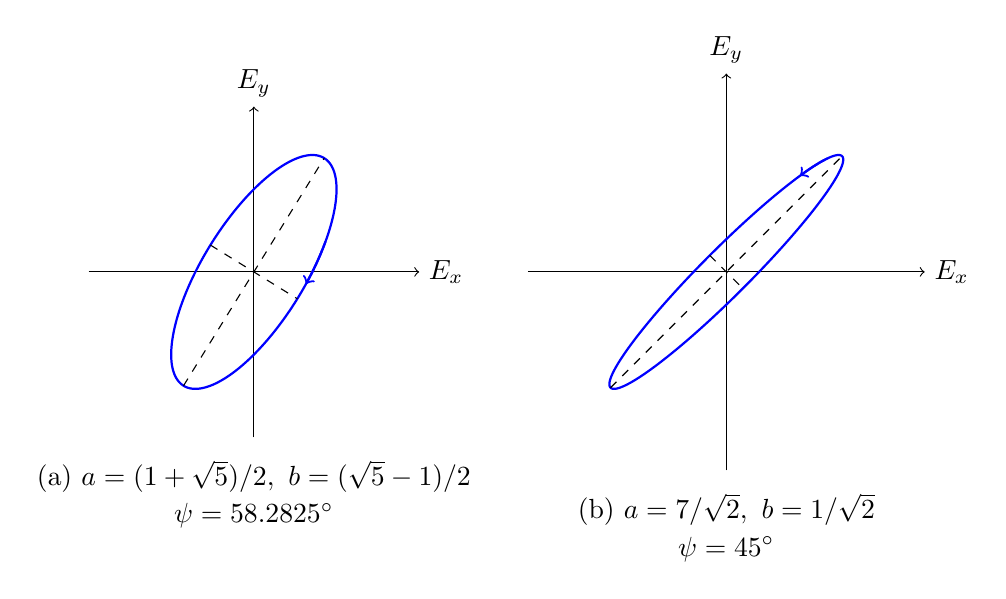
\begin{tikzpicture}
\begin{scope}[xshift=0cm,scale=1.05]
\draw[->] (-2.0,0)--(2.0,0) node[right] {$E_x$};
\draw[->] (0,-2.0)--(0,2.0) node[above] {$E_y$};
\draw[blue,thick] plot coordinates {(1.000000,1.000000) (0.999657,0.973480) (0.998630,0.946294) (0.996917,0.918458) (0.994522,0.889993) (0.991445,0.860919) (0.987688,0.831254) (0.983255,0.801019) (0.978148,0.770236) (0.972370,0.738925) (0.965926,0.707107) (0.958820,0.674804) (0.951057,0.642040) (0.942641,0.608835) (0.933580,0.575212) (0.923880,0.541196) (0.913545,0.506809) (0.902585,0.472074) (0.891007,0.437016) (0.878817,0.401658) (0.866025,0.366025) (0.852640,0.330142) (0.838671,0.294032) (0.824126,0.257720) (0.809017,0.221232) (0.793353,0.184592) (0.777146,0.147826) (0.760406,0.110958) (0.743145,0.074014) (0.725374,0.037020) (0.707107,0.000000) (0.688355,-0.037020) (0.669131,-0.074014) (0.649448,-0.110958) (0.629320,-0.147826) (0.608761,-0.184592) (0.587785,-0.221232) (0.566406,-0.257720) (0.544639,-0.294032) (0.522499,-0.330142) (0.500000,-0.366025) (0.477159,-0.401658) (0.453990,-0.437016) (0.430511,-0.472074) (0.406737,-0.506809) (0.382683,-0.541196) (0.358368,-0.575212) (0.333807,-0.608835) (0.309017,-0.642040) (0.284015,-0.674804) (0.258819,-0.707107) (0.233445,-0.738925) (0.207912,-0.770236) (0.182236,-0.801019) (0.156434,-0.831254) (0.130526,-0.860919) (0.104528,-0.889993) (0.078459,-0.918458) (0.052336,-0.946294) (0.026177,-0.973480) (0.000000,-1.000000) (-0.026177,-1.025834) (-0.052336,-1.050965) (-0.078459,-1.075376) (-0.104528,-1.099050) (-0.130526,-1.121971) (-0.156434,-1.144123) (-0.182236,-1.165490) (-0.207912,-1.186059) (-0.233445,-1.205815) (-0.258819,-1.224745) (-0.284015,-1.242835) (-0.309017,-1.260074) (-0.333807,-1.276448) (-0.358368,-1.291948) (-0.382683,-1.306563) (-0.406737,-1.320282) (-0.430511,-1.333096) (-0.453990,-1.344997) (-0.477159,-1.355976) (-0.500000,-1.366025) (-0.522499,-1.375139) (-0.544639,-1.383310) (-0.566406,-1.390532) (-0.587785,-1.396802) (-0.608761,-1.402115) (-0.629320,-1.406466) (-0.649448,-1.409854) (-0.669131,-1.412275) (-0.688355,-1.413729) (-0.707107,-1.414214) (-0.725374,-1.413729) (-0.743145,-1.412275) (-0.760406,-1.409854) (-0.777146,-1.406466) (-0.793353,-1.402115) (-0.809017,-1.396802) (-0.824126,-1.390532) (-0.838671,-1.383310) (-0.852640,-1.375139) (-0.866025,-1.366025) (-0.878817,-1.355976) (-0.891007,-1.344997) (-0.902585,-1.333096) (-0.913545,-1.320282) (-0.923880,-1.306563) (-0.933580,-1.291948) (-0.942641,-1.276448) (-0.951057,-1.260074) (-0.958820,-1.242835) (-0.965926,-1.224745) (-0.972370,-1.205815) (-0.978148,-1.186059) (-0.983255,-1.165490) (-0.987688,-1.144123) (-0.991445,-1.121971) (-0.994522,-1.099050) (-0.996917,-1.075376) (-0.998630,-1.050965) (-0.999657,-1.025834) (-1.000000,-1.000000) (-0.999657,-0.973480) (-0.998630,-0.946294) (-0.996917,-0.918458) (-0.994522,-0.889993) (-0.991445,-0.860919) (-0.987688,-0.831254) (-0.983255,-0.801019) (-0.978148,-0.770236) (-0.972370,-0.738925) (-0.965926,-0.707107) (-0.958820,-0.674804) (-0.951057,-0.642040) (-0.942641,-0.608835) (-0.933580,-0.575212) (-0.923880,-0.541196) (-0.913545,-0.506809) (-0.902585,-0.472074) (-0.891007,-0.437016) (-0.878817,-0.401658) (-0.866025,-0.366025) (-0.852640,-0.330142) (-0.838671,-0.294032) (-0.824126,-0.257720) (-0.809017,-0.221232) (-0.793353,-0.184592) (-0.777146,-0.147826) (-0.760406,-0.110958) (-0.743145,-0.074014) (-0.725374,-0.037020) (-0.707107,-0.000000) (-0.688355,0.037020) (-0.669131,0.074014) (-0.649448,0.110958) (-0.629320,0.147826) (-0.608761,0.184592) (-0.587785,0.221232) (-0.566406,0.257720) (-0.544639,0.294032) (-0.522499,0.330142) (-0.500000,0.366025) (-0.477159,0.401658) (-0.453990,0.437016) (-0.430511,0.472074) (-0.406737,0.506809) (-0.382683,0.541196) (-0.358368,0.575212) (-0.333807,0.608835) (-0.309017,0.642040) (-0.284015,0.674804) (-0.258819,0.707107) (-0.233445,0.738925) (-0.207912,0.770236) (-0.182236,0.801019) (-0.156434,0.831254) (-0.130526,0.860919) (-0.104528,0.889993) (-0.078459,0.918458) (-0.052336,0.946294) (-0.026177,0.973480) (-0.000000,1.000000) (0.026177,1.025834) (0.052336,1.050965) (0.078459,1.075376) (0.104528,1.099050) (0.130526,1.121971) (0.156434,1.144123) (0.182236,1.165490) (0.207912,1.186059) (0.233445,1.205815) (0.258819,1.224745) (0.284015,1.242835) (0.309017,1.260074) (0.333807,1.276448) (0.358368,1.291948) (0.382683,1.306563) (0.406737,1.320282) (0.430511,1.333096) (0.453990,1.344997) (0.477159,1.355976) (0.500000,1.366025) (0.522499,1.375139) (0.544639,1.383310) (0.566406,1.390532) (0.587785,1.396802) (0.608761,1.402115) (0.629320,1.406466) (0.649448,1.409854) (0.669131,1.412275) (0.688355,1.413729) (0.707107,1.414214) (0.725374,1.413729) (0.743145,1.412275) (0.760406,1.409854) (0.777146,1.406466) (0.793353,1.402115) (0.809017,1.396802) (0.824126,1.390532) (0.838671,1.383310) (0.852640,1.375139) (0.866025,1.366025) (0.878817,1.355976) (0.891007,1.344997) (0.902585,1.333096) (0.913545,1.320282) (0.923880,1.306563) (0.933580,1.291948) (0.942641,1.276448) (0.951057,1.260074) (0.958820,1.242835) (0.965926,1.224745) (0.972370,1.205815) (0.978148,1.186059) (0.983255,1.165490) (0.987688,1.144123) (0.991445,1.121971) (0.994522,1.099050) (0.996917,1.075376) (0.998630,1.050965) (0.999657,1.025834) (1.000000,1.000000)};
\draw[blue,->,thick] plot coordinates {(0.866025,0.366025) (0.852640,0.330142) (0.838671,0.294032) (0.824126,0.257720) (0.809017,0.221232) (0.793353,0.184592) (0.777146,0.147826) (0.760406,0.110958) (0.743145,0.074014) (0.725374,0.037020) (0.707107,0.000000) (0.688355,-0.037020) (0.669131,-0.074014) (0.649448,-0.110958) (0.629320,-0.147826)};
\draw[black,dashed] plot coordinates {(-0.525731,0.324920) (0.525731,-0.324920)};
\draw[black,dashed] plot coordinates {(-0.850651,-1.376382) (0.850651,1.376382)};
\node at (0,-2.4761904761904763) {(a) $a=(1+\sqrt5)/2,\ b=(\sqrt5-1)/2$};
\node at (0,-2.9523809523809526) {$\psi=58.2825^\circ$};
\end{scope}
\begin{scope}[xshift=6cm,scale=0.42]
\draw[->] (-6.0,0)--(6.0,0) node[right] {$E_x$};
\draw[->] (0,-6.0)--(0,6.0) node[above] {$E_y$};
\draw[blue,thick] plot coordinates {(3.535534,3.394113) (3.534322,3.418863) (3.530689,3.441271) (3.524635,3.461320) (3.516166,3.478997) (3.505287,3.494290) (3.492006,3.507188) (3.476331,3.517682) (3.458274,3.525765) (3.437847,3.531432) (3.415064,3.534679) (3.389940,3.535503) (3.362493,3.533904) (3.332741,3.529883) (3.300705,3.523443) (3.266407,3.514588) (3.229871,3.503325) (3.191121,3.489660) (3.150184,3.473604) (3.107088,3.455167) (3.061862,3.434362) (3.014538,3.411204) (2.965148,3.385707) (2.913726,3.357891) (2.860307,3.327772) (2.804928,3.295374) (2.747626,3.260716) (2.688441,3.223824) (2.627414,3.184723) (2.564586,3.143439) (2.500000,3.100000) (2.433701,3.054437) (2.365734,3.006780) (2.296146,2.957063) (2.224984,2.905319) (2.152297,2.851585) (2.078135,2.795895) (2.002548,2.738290) (1.925590,2.678808) (1.847311,2.617490) (1.767767,2.554378) (1.687011,2.489515) (1.605099,2.422946) (1.522087,2.354717) (1.438031,2.284874) (1.352990,2.213465) (1.267022,2.140539) (1.180185,2.066146) (1.092540,1.990336) (1.004146,1.913163) (0.915064,1.834679) (0.825354,1.754937) (0.735079,1.673992) (0.644300,1.591901) (0.553079,1.508718) (0.461480,1.424501) (0.369564,1.339308) (0.277395,1.253197) (0.185036,1.166227) (0.092549,1.078458) (0.000000,0.989949) (-0.092549,0.900763) (-0.185036,0.810959) (-0.277395,0.720599) (-0.369564,0.629745) (-0.461480,0.538460) (-0.553079,0.446805) (-0.644300,0.354845) (-0.735079,0.262641) (-0.825354,0.170257) (-0.915064,0.077757) (-1.004146,-0.014797) (-1.092540,-0.107341) (-1.180185,-0.199811) (-1.267022,-0.292144) (-1.352990,-0.384277) (-1.438031,-0.476146) (-1.522087,-0.567689) (-1.605099,-0.658843) (-1.687011,-0.749546) (-1.767767,-0.839735) (-1.847311,-0.929348) (-1.925590,-1.018325) (-2.002548,-1.106603) (-2.078135,-1.194123) (-2.152297,-1.280825) (-2.224984,-1.366649) (-2.296146,-1.451536) (-2.365734,-1.535429) (-2.433701,-1.618269) (-2.500000,-1.700000) (-2.564586,-1.780566) (-2.627414,-1.859912) (-2.688441,-1.937983) (-2.747626,-2.014725) (-2.804928,-2.090087) (-2.860307,-2.164017) (-2.913726,-2.236463) (-2.965148,-2.307377) (-3.014538,-2.376709) (-3.061862,-2.444413) (-3.107088,-2.510441) (-3.150184,-2.574749) (-3.191121,-2.637292) (-3.229871,-2.698027) (-3.266407,-2.756914) (-3.300705,-2.813911) (-3.332741,-2.868979) (-3.362493,-2.922082) (-3.389940,-2.973181) (-3.415064,-3.022243) (-3.437847,-3.069234) (-3.458274,-3.114121) (-3.476331,-3.156874) (-3.492006,-3.197463) (-3.505287,-3.235861) (-3.516166,-3.272041) (-3.524635,-3.305979) (-3.530689,-3.337651) (-3.534322,-3.367036) (-3.535534,-3.394113) (-3.534322,-3.418863) (-3.530689,-3.441271) (-3.524635,-3.461320) (-3.516166,-3.478997) (-3.505287,-3.494290) (-3.492006,-3.507188) (-3.476331,-3.517682) (-3.458274,-3.525765) (-3.437847,-3.531432) (-3.415064,-3.534679) (-3.389940,-3.535503) (-3.362493,-3.533904) (-3.332741,-3.529883) (-3.300705,-3.523443) (-3.266407,-3.514588) (-3.229871,-3.503325) (-3.191121,-3.489660) (-3.150184,-3.473604) (-3.107088,-3.455167) (-3.061862,-3.434362) (-3.014538,-3.411204) (-2.965148,-3.385707) (-2.913726,-3.357891) (-2.860307,-3.327772) (-2.804928,-3.295374) (-2.747626,-3.260716) (-2.688441,-3.223824) (-2.627414,-3.184723) (-2.564586,-3.143439) (-2.500000,-3.100000) (-2.433701,-3.054437) (-2.365734,-3.006780) (-2.296146,-2.957063) (-2.224984,-2.905319) (-2.152297,-2.851585) (-2.078135,-2.795895) (-2.002548,-2.738290) (-1.925590,-2.678808) (-1.847311,-2.617490) (-1.767767,-2.554378) (-1.687011,-2.489515) (-1.605099,-2.422946) (-1.522087,-2.354717) (-1.438031,-2.284874) (-1.352990,-2.213465) (-1.267022,-2.140539) (-1.180185,-2.066146) (-1.092540,-1.990336) (-1.004146,-1.913163) (-0.915064,-1.834679) (-0.825354,-1.754937) (-0.735079,-1.673992) (-0.644300,-1.591901) (-0.553079,-1.508718) (-0.461480,-1.424501) (-0.369564,-1.339308) (-0.277395,-1.253197) (-0.185036,-1.166227) (-0.092549,-1.078458) (-0.000000,-0.989949) (0.092549,-0.900763) (0.185036,-0.810959) (0.277395,-0.720599) (0.369564,-0.629745) (0.461480,-0.538460) (0.553079,-0.446805) (0.644300,-0.354845) (0.735079,-0.262641) (0.825354,-0.170257) (0.915064,-0.077757) (1.004146,0.014797) (1.092540,0.107341) (1.180185,0.199811) (1.267022,0.292144) (1.352990,0.384277) (1.438031,0.476146) (1.522087,0.567689) (1.605099,0.658843) (1.687011,0.749546) (1.767767,0.839735) (1.847311,0.929348) (1.925590,1.018325) (2.002548,1.106603) (2.078135,1.194123) (2.152297,1.280825) (2.224984,1.366649) (2.296146,1.451536) (2.365734,1.535429) (2.433701,1.618269) (2.500000,1.700000) (2.564586,1.780566) (2.627414,1.859912) (2.688441,1.937983) (2.747626,2.014725) (2.804928,2.090087) (2.860307,2.164017) (2.913726,2.236463) (2.965148,2.307377) (3.014538,2.376709) (3.061862,2.444413) (3.107088,2.510441) (3.150184,2.574749) (3.191121,2.637292) (3.229871,2.698027) (3.266407,2.756914) (3.300705,2.813911) (3.332741,2.868979) (3.362493,2.922082) (3.389940,2.973181) (3.415064,3.022243) (3.437847,3.069234) (3.458274,3.114121) (3.476331,3.156874) (3.492006,3.197463) (3.505287,3.235861) (3.516166,3.272041) (3.524635,3.305979) (3.530689,3.337651) (3.534322,3.367036) (3.535534,3.394113)};
\draw[blue,->,thick] plot coordinates {(3.061862,3.434362) (3.014538,3.411204) (2.965148,3.385707) (2.913726,3.357891) (2.860307,3.327772) (2.804928,3.295374) (2.747626,3.260716) (2.688441,3.223824) (2.627414,3.184723) (2.564586,3.143439) (2.500000,3.100000) (2.433701,3.054437) (2.365734,3.006780) (2.296146,2.957063) (2.224984,2.905319)};
\draw[black,dashed] plot coordinates {(-0.500000,0.500000) (0.500000,-0.500000)};
\draw[black,dashed] plot coordinates {(-3.500000,-3.500000) (3.500000,3.500000)};
\node at (0,-7.190476190476191) {(b) $a=7/\sqrt2,\ b=1/\sqrt2$};
\node at (0,-8.380952380952381) {$\psi=45^\circ$};
\end{scope}
\end{tikzpicture}

\end{center}

\Needspace{5\baselineskip}
\par\bigskip
\noindent\textbf{7.2}\quad A plane wave is incident on a layered interface as shown in the figure. The indices of refraction of the three nonpermeable media are $n_{1}$, $n_{2}$, $n_{3}$. The thickness of the intermediate layer is $d$. Each of the other media is semi-infinite.
\begin{enumerate}
\item[(a)] Calculate the transmission and reflection coefficients (ratios of transmitted and reflected Poynting's flux to the incident flux), and sketch their behavior as a function of frequency for $n_{1}=1$, $n_{2}=2$, $n_{3}=3$; $n_{1}=3$, $n_{2}=2$, $n_{3}=1$; and $n_{1}=2$, $n_{2}=4$, $n_{3}=1$.
\end{enumerate}

\begin{center}
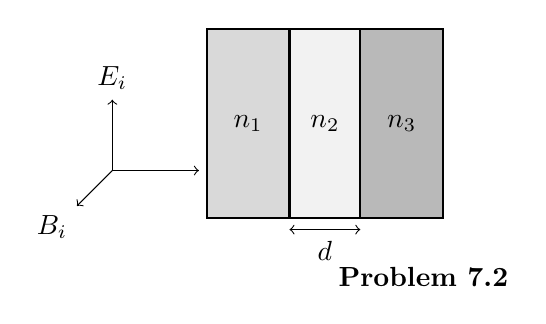
\begin{tikzpicture}[scale=1.0]
  % slab n1 (left, medium shading)
  \fill[gray!30] (-1.4,0) rectangle (-0.35,2.4);
  \draw[thick] (-1.4,0) rectangle (-0.35,2.4);
  \node at (-0.875,1.2) {$n_{1}$};
  % slab n2 (middle, light)
  \fill[gray!10] (-0.35,0) rectangle (0.55,2.4);
  \draw[thick] (-0.35,0) rectangle (0.55,2.4);
  \node at (0.1,1.2) {$n_{2}$};
  % slab n3 (right, dark)
  \fill[gray!55] (0.55,0) rectangle (1.6,2.4);
  \draw[thick] (0.55,0) rectangle (1.6,2.4);
  \node at (1.075,1.2) {$n_{3}$};
  % d dimension below n2
  \draw[<->] (-0.35,-0.15) -- (0.55,-0.15);
  \node[below] at (0.1,-0.18) {$d$};
  % incident ray coordinate axes at left
  \draw[->] (-2.6,0.6) -- (-1.5,0.6);
  \draw[->] (-2.6,0.6) -- (-2.6,1.5) node[above] {$E_{i}$};
  \draw[->] (-2.6,0.6) -- (-3.05,0.15) node[below left] {$B_{i}$};
  \node at (1.35,-0.75) {\textbf{Problem 7.2}};
\end{tikzpicture}
\end{center}

\begin{enumerate}
\item[(b)] The medium $n_{1}$ is part of an optical system (e.g., a lens); medium $n_{3}$ is air ($n_{3}=1$). It is desired to put an optical coating (medium $n_{2}$) on the surface so that there is no reflected wave for a frequency $\omega_{0}$. What thickness $d$ and index of refraction $n_{2}$ are necessary?
\end{enumerate}
\solution
The drawing specifies normal incidence. Take $e^{-i\omega t}$ time
dependence, and reference incident/reflected amplitudes to the first
face and the transmitted amplitude to the second face. Define
\[
r_{ij}=\frac{n_i-n_j}{n_i+n_j},\quad
 t_{ij}=\frac{2n_i}{n_i+n_j},\quad \delta=\frac{n_2\omega d}{c}.
\]
At either face continuity of $E_t,H_t$ gives
$E_i+E_r=E_t$ and $n_i(E_i-E_r)=n_jE_t$, proving these single-face
coefficients.
\textbf{(a)} A round trip inside the film multiplies an amplitude by
$r_{21}r_{23}e^{2i\delta}=-r_{12}r_{23}e^{2i\delta}$.
Summing all transmitted trips therefore gives
\[
t=\frac{t_{12}t_{23}e^{i\delta}}{1+r_{12}r_{23}e^{2i\delta}}.
\]
The direct reflection plus the waves returned through the first
face gives
\[
r=r_{12}+\frac{t_{12}t_{21}r_{23}e^{2i\delta}}
 {1+r_{12}r_{23}e^{2i\delta}}
=\frac{r_{12}+r_{23}e^{2i\delta}}{1+r_{12}r_{23}e^{2i\delta}},
\]
where $t_{12}t_{21}=1-r_{12}^2$ was used. Since the flux for a
traveling electric amplitude is $n|E|^2/(2Z_0)$,
\[
\boxed{R=|r|^2,\qquad T=\frac{n_3}{n_1}|t|^2.}
\]
A useful real form, obtained by multiplying the denominator by
$e^{-i\delta}$, is
\[
\boxed{T=\frac{4n_1n_3}
 {(n_1+n_3)^2\cos^2\delta+(n_2+n_1n_3/n_2)^2\sin^2\delta},
\qquad R=1-T.}
\]
Indeed the numerator of $R$ is the same denominator minus $4n_1n_3$,
namely $(n_1-n_3)^2\cos^2\delta+(n_2-n_1n_3/n_2)^2\sin^2\delta$.
For $(n_1,n_2,n_3)=(1,2,3)$ and $(3,2,1)$ the flux curves coincide:
\[
T=\frac{12}{16\cos^2\delta+(49/4)\sin^2\delta},\qquad
\frac34\leq T\leq\frac{48}{49}.
\]
For $(2,4,1)$,
\[
T=\frac8{9\cos^2\delta+(81/4)\sin^2\delta},\qquad
\frac{32}{81}\leq T\leq\frac89.
\]
The plot uses a common frequency coordinate $\omega d/(\pi c)$,
so the third film has twice as many fringes as the first two.
\begin{center}
% Generated by supplementary/check_ch07.py --write-assets
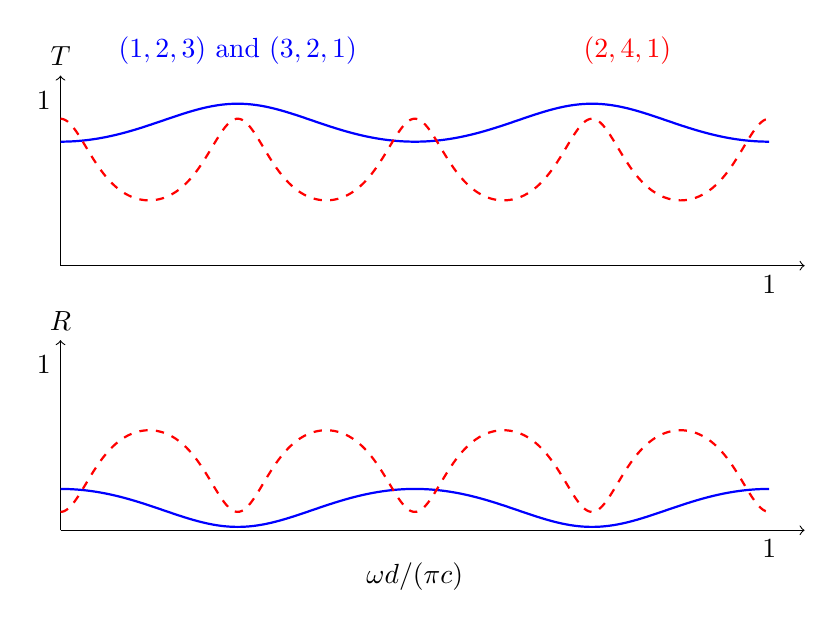
\begin{tikzpicture}[x=9cm,y=2.1cm]
\begin{scope}[yshift=0.0cm]
\draw[->] (0,0)--(1.05,0);\draw[->] (0,0)--(0,1.15) node[above] {$T$};
\draw[blue,thick] plot coordinates {(0.000000,0.750000) (0.002500,0.750043) (0.005000,0.750173) (0.007500,0.750390) (0.010000,0.750694) (0.012500,0.751084) (0.015000,0.751560) (0.017500,0.752123) (0.020000,0.752771) (0.022500,0.753506) (0.025000,0.754326) (0.027500,0.755232) (0.030000,0.756223) (0.032500,0.757299) (0.035000,0.758459) (0.037500,0.759703) (0.040000,0.761031) (0.042500,0.762443) (0.045000,0.763936) (0.047500,0.765512) (0.050000,0.767170) (0.052500,0.768908) (0.055000,0.770727) (0.057500,0.772625) (0.060000,0.774603) (0.062500,0.776658) (0.065000,0.778790) (0.067500,0.780998) (0.070000,0.783281) (0.072500,0.785638) (0.075000,0.788069) (0.077500,0.790571) (0.080000,0.793143) (0.082500,0.795785) (0.085000,0.798494) (0.087500,0.801270) (0.090000,0.804110) (0.092500,0.807013) (0.095000,0.809977) (0.097500,0.813001) (0.100000,0.816082) (0.102500,0.819218) (0.105000,0.822408) (0.107500,0.825649) (0.110000,0.828939) (0.112500,0.832275) (0.115000,0.835655) (0.117500,0.839076) (0.120000,0.842535) (0.122500,0.846030) (0.125000,0.849558) (0.127500,0.853115) (0.130000,0.856698) (0.132500,0.860305) (0.135000,0.863931) (0.137500,0.867573) (0.140000,0.871228) (0.142500,0.874892) (0.145000,0.878561) (0.147500,0.882230) (0.150000,0.885897) (0.152500,0.889557) (0.155000,0.893205) (0.157500,0.896838) (0.160000,0.900450) (0.162500,0.904039) (0.165000,0.907598) (0.167500,0.911124) (0.170000,0.914612) (0.172500,0.918056) (0.175000,0.921454) (0.177500,0.924799) (0.180000,0.928086) (0.182500,0.931313) (0.185000,0.934472) (0.187500,0.937560) (0.190000,0.940573) (0.192500,0.943504) (0.195000,0.946351) (0.197500,0.949107) (0.200000,0.951770) (0.202500,0.954333) (0.205000,0.956794) (0.207500,0.959148) (0.210000,0.961390) (0.212500,0.963518) (0.215000,0.965527) (0.217500,0.967413) (0.220000,0.969175) (0.222500,0.970807) (0.225000,0.972308) (0.227500,0.973674) (0.230000,0.974904) (0.232500,0.975994) (0.235000,0.976943) (0.237500,0.977749) (0.240000,0.978411) (0.242500,0.978927) (0.245000,0.979296) (0.247500,0.979518) (0.250000,0.979592) (0.252500,0.979518) (0.255000,0.979296) (0.257500,0.978927) (0.260000,0.978411) (0.262500,0.977749) (0.265000,0.976943) (0.267500,0.975994) (0.270000,0.974904) (0.272500,0.973674) (0.275000,0.972308) (0.277500,0.970807) (0.280000,0.969175) (0.282500,0.967413) (0.285000,0.965527) (0.287500,0.963518) (0.290000,0.961390) (0.292500,0.959148) (0.295000,0.956794) (0.297500,0.954333) (0.300000,0.951770) (0.302500,0.949107) (0.305000,0.946351) (0.307500,0.943504) (0.310000,0.940573) (0.312500,0.937560) (0.315000,0.934472) (0.317500,0.931313) (0.320000,0.928086) (0.322500,0.924799) (0.325000,0.921454) (0.327500,0.918056) (0.330000,0.914612) (0.332500,0.911124) (0.335000,0.907598) (0.337500,0.904039) (0.340000,0.900450) (0.342500,0.896838) (0.345000,0.893205) (0.347500,0.889557) (0.350000,0.885897) (0.352500,0.882230) (0.355000,0.878561) (0.357500,0.874892) (0.360000,0.871228) (0.362500,0.867573) (0.365000,0.863931) (0.367500,0.860305) (0.370000,0.856698) (0.372500,0.853115) (0.375000,0.849558) (0.377500,0.846030) (0.380000,0.842535) (0.382500,0.839076) (0.385000,0.835655) (0.387500,0.832275) (0.390000,0.828939) (0.392500,0.825649) (0.395000,0.822408) (0.397500,0.819218) (0.400000,0.816082) (0.402500,0.813001) (0.405000,0.809977) (0.407500,0.807013) (0.410000,0.804110) (0.412500,0.801270) (0.415000,0.798494) (0.417500,0.795785) (0.420000,0.793143) (0.422500,0.790571) (0.425000,0.788069) (0.427500,0.785638) (0.430000,0.783281) (0.432500,0.780998) (0.435000,0.778790) (0.437500,0.776658) (0.440000,0.774603) (0.442500,0.772625) (0.445000,0.770727) (0.447500,0.768908) (0.450000,0.767170) (0.452500,0.765512) (0.455000,0.763936) (0.457500,0.762443) (0.460000,0.761031) (0.462500,0.759703) (0.465000,0.758459) (0.467500,0.757299) (0.470000,0.756223) (0.472500,0.755232) (0.475000,0.754326) (0.477500,0.753506) (0.480000,0.752771) (0.482500,0.752123) (0.485000,0.751560) (0.487500,0.751084) (0.490000,0.750694) (0.492500,0.750390) (0.495000,0.750173) (0.497500,0.750043) (0.500000,0.750000) (0.502500,0.750043) (0.505000,0.750173) (0.507500,0.750390) (0.510000,0.750694) (0.512500,0.751084) (0.515000,0.751560) (0.517500,0.752123) (0.520000,0.752771) (0.522500,0.753506) (0.525000,0.754326) (0.527500,0.755232) (0.530000,0.756223) (0.532500,0.757299) (0.535000,0.758459) (0.537500,0.759703) (0.540000,0.761031) (0.542500,0.762443) (0.545000,0.763936) (0.547500,0.765512) (0.550000,0.767170) (0.552500,0.768908) (0.555000,0.770727) (0.557500,0.772625) (0.560000,0.774603) (0.562500,0.776658) (0.565000,0.778790) (0.567500,0.780998) (0.570000,0.783281) (0.572500,0.785638) (0.575000,0.788069) (0.577500,0.790571) (0.580000,0.793143) (0.582500,0.795785) (0.585000,0.798494) (0.587500,0.801270) (0.590000,0.804110) (0.592500,0.807013) (0.595000,0.809977) (0.597500,0.813001) (0.600000,0.816082) (0.602500,0.819218) (0.605000,0.822408) (0.607500,0.825649) (0.610000,0.828939) (0.612500,0.832275) (0.615000,0.835655) (0.617500,0.839076) (0.620000,0.842535) (0.622500,0.846030) (0.625000,0.849558) (0.627500,0.853115) (0.630000,0.856698) (0.632500,0.860305) (0.635000,0.863931) (0.637500,0.867573) (0.640000,0.871228) (0.642500,0.874892) (0.645000,0.878561) (0.647500,0.882230) (0.650000,0.885897) (0.652500,0.889557) (0.655000,0.893205) (0.657500,0.896838) (0.660000,0.900450) (0.662500,0.904039) (0.665000,0.907598) (0.667500,0.911124) (0.670000,0.914612) (0.672500,0.918056) (0.675000,0.921454) (0.677500,0.924799) (0.680000,0.928086) (0.682500,0.931313) (0.685000,0.934472) (0.687500,0.937560) (0.690000,0.940573) (0.692500,0.943504) (0.695000,0.946351) (0.697500,0.949107) (0.700000,0.951770) (0.702500,0.954333) (0.705000,0.956794) (0.707500,0.959148) (0.710000,0.961390) (0.712500,0.963518) (0.715000,0.965527) (0.717500,0.967413) (0.720000,0.969175) (0.722500,0.970807) (0.725000,0.972308) (0.727500,0.973674) (0.730000,0.974904) (0.732500,0.975994) (0.735000,0.976943) (0.737500,0.977749) (0.740000,0.978411) (0.742500,0.978927) (0.745000,0.979296) (0.747500,0.979518) (0.750000,0.979592) (0.752500,0.979518) (0.755000,0.979296) (0.757500,0.978927) (0.760000,0.978411) (0.762500,0.977749) (0.765000,0.976943) (0.767500,0.975994) (0.770000,0.974904) (0.772500,0.973674) (0.775000,0.972308) (0.777500,0.970807) (0.780000,0.969175) (0.782500,0.967413) (0.785000,0.965527) (0.787500,0.963518) (0.790000,0.961390) (0.792500,0.959148) (0.795000,0.956794) (0.797500,0.954333) (0.800000,0.951770) (0.802500,0.949107) (0.805000,0.946351) (0.807500,0.943504) (0.810000,0.940573) (0.812500,0.937560) (0.815000,0.934472) (0.817500,0.931313) (0.820000,0.928086) (0.822500,0.924799) (0.825000,0.921454) (0.827500,0.918056) (0.830000,0.914612) (0.832500,0.911124) (0.835000,0.907598) (0.837500,0.904039) (0.840000,0.900450) (0.842500,0.896838) (0.845000,0.893205) (0.847500,0.889557) (0.850000,0.885897) (0.852500,0.882230) (0.855000,0.878561) (0.857500,0.874892) (0.860000,0.871228) (0.862500,0.867573) (0.865000,0.863931) (0.867500,0.860305) (0.870000,0.856698) (0.872500,0.853115) (0.875000,0.849558) (0.877500,0.846030) (0.880000,0.842535) (0.882500,0.839076) (0.885000,0.835655) (0.887500,0.832275) (0.890000,0.828939) (0.892500,0.825649) (0.895000,0.822408) (0.897500,0.819218) (0.900000,0.816082) (0.902500,0.813001) (0.905000,0.809977) (0.907500,0.807013) (0.910000,0.804110) (0.912500,0.801270) (0.915000,0.798494) (0.917500,0.795785) (0.920000,0.793143) (0.922500,0.790571) (0.925000,0.788069) (0.927500,0.785638) (0.930000,0.783281) (0.932500,0.780998) (0.935000,0.778790) (0.937500,0.776658) (0.940000,0.774603) (0.942500,0.772625) (0.945000,0.770727) (0.947500,0.768908) (0.950000,0.767170) (0.952500,0.765512) (0.955000,0.763936) (0.957500,0.762443) (0.960000,0.761031) (0.962500,0.759703) (0.965000,0.758459) (0.967500,0.757299) (0.970000,0.756223) (0.972500,0.755232) (0.975000,0.754326) (0.977500,0.753506) (0.980000,0.752771) (0.982500,0.752123) (0.985000,0.751560) (0.987500,0.751084) (0.990000,0.750694) (0.992500,0.750390) (0.995000,0.750173) (0.997500,0.750043) (1.000000,0.750000)};
\draw[red,dashed,thick] plot coordinates {(0.000000,0.888889) (0.002500,0.887794) (0.005000,0.884530) (0.007500,0.879156) (0.010000,0.871771) (0.012500,0.862505) (0.015000,0.851516) (0.017500,0.838984) (0.020000,0.825102) (0.022500,0.810073) (0.025000,0.794101) (0.027500,0.777389) (0.030000,0.760127) (0.032500,0.742499) (0.035000,0.724671) (0.037500,0.706794) (0.040000,0.689003) (0.042500,0.671415) (0.045000,0.654130) (0.047500,0.637232) (0.050000,0.620791) (0.052500,0.604864) (0.055000,0.589493) (0.057500,0.574713) (0.060000,0.560546) (0.062500,0.547009) (0.065000,0.534110) (0.067500,0.521853) (0.070000,0.510236) (0.072500,0.499255) (0.075000,0.488901) (0.077500,0.479165) (0.080000,0.470035) (0.082500,0.461498) (0.085000,0.453540) (0.087500,0.446147) (0.090000,0.439307) (0.092500,0.433004) (0.095000,0.427226) (0.097500,0.421960) (0.100000,0.417194) (0.102500,0.412917) (0.105000,0.409119) (0.107500,0.405790) (0.110000,0.402921) (0.112500,0.400507) (0.115000,0.398540) (0.117500,0.397015) (0.120000,0.395929) (0.122500,0.395278) (0.125000,0.395062) (0.127500,0.395278) (0.130000,0.395929) (0.132500,0.397015) (0.135000,0.398540) (0.137500,0.400507) (0.140000,0.402921) (0.142500,0.405790) (0.145000,0.409119) (0.147500,0.412917) (0.150000,0.417194) (0.152500,0.421960) (0.155000,0.427226) (0.157500,0.433004) (0.160000,0.439307) (0.162500,0.446147) (0.165000,0.453540) (0.167500,0.461498) (0.170000,0.470035) (0.172500,0.479165) (0.175000,0.488901) (0.177500,0.499255) (0.180000,0.510236) (0.182500,0.521853) (0.185000,0.534110) (0.187500,0.547009) (0.190000,0.560546) (0.192500,0.574713) (0.195000,0.589493) (0.197500,0.604864) (0.200000,0.620791) (0.202500,0.637232) (0.205000,0.654130) (0.207500,0.671415) (0.210000,0.689003) (0.212500,0.706794) (0.215000,0.724671) (0.217500,0.742499) (0.220000,0.760127) (0.222500,0.777389) (0.225000,0.794101) (0.227500,0.810073) (0.230000,0.825102) (0.232500,0.838984) (0.235000,0.851516) (0.237500,0.862505) (0.240000,0.871771) (0.242500,0.879156) (0.245000,0.884530) (0.247500,0.887794) (0.250000,0.888889) (0.252500,0.887794) (0.255000,0.884530) (0.257500,0.879156) (0.260000,0.871771) (0.262500,0.862505) (0.265000,0.851516) (0.267500,0.838984) (0.270000,0.825102) (0.272500,0.810073) (0.275000,0.794101) (0.277500,0.777389) (0.280000,0.760127) (0.282500,0.742499) (0.285000,0.724671) (0.287500,0.706794) (0.290000,0.689003) (0.292500,0.671415) (0.295000,0.654130) (0.297500,0.637232) (0.300000,0.620791) (0.302500,0.604864) (0.305000,0.589493) (0.307500,0.574713) (0.310000,0.560546) (0.312500,0.547009) (0.315000,0.534110) (0.317500,0.521853) (0.320000,0.510236) (0.322500,0.499255) (0.325000,0.488901) (0.327500,0.479165) (0.330000,0.470035) (0.332500,0.461498) (0.335000,0.453540) (0.337500,0.446147) (0.340000,0.439307) (0.342500,0.433004) (0.345000,0.427226) (0.347500,0.421960) (0.350000,0.417194) (0.352500,0.412917) (0.355000,0.409119) (0.357500,0.405790) (0.360000,0.402921) (0.362500,0.400507) (0.365000,0.398540) (0.367500,0.397015) (0.370000,0.395929) (0.372500,0.395278) (0.375000,0.395062) (0.377500,0.395278) (0.380000,0.395929) (0.382500,0.397015) (0.385000,0.398540) (0.387500,0.400507) (0.390000,0.402921) (0.392500,0.405790) (0.395000,0.409119) (0.397500,0.412917) (0.400000,0.417194) (0.402500,0.421960) (0.405000,0.427226) (0.407500,0.433004) (0.410000,0.439307) (0.412500,0.446147) (0.415000,0.453540) (0.417500,0.461498) (0.420000,0.470035) (0.422500,0.479165) (0.425000,0.488901) (0.427500,0.499255) (0.430000,0.510236) (0.432500,0.521853) (0.435000,0.534110) (0.437500,0.547009) (0.440000,0.560546) (0.442500,0.574713) (0.445000,0.589493) (0.447500,0.604864) (0.450000,0.620791) (0.452500,0.637232) (0.455000,0.654130) (0.457500,0.671415) (0.460000,0.689003) (0.462500,0.706794) (0.465000,0.724671) (0.467500,0.742499) (0.470000,0.760127) (0.472500,0.777389) (0.475000,0.794101) (0.477500,0.810073) (0.480000,0.825102) (0.482500,0.838984) (0.485000,0.851516) (0.487500,0.862505) (0.490000,0.871771) (0.492500,0.879156) (0.495000,0.884530) (0.497500,0.887794) (0.500000,0.888889) (0.502500,0.887794) (0.505000,0.884530) (0.507500,0.879156) (0.510000,0.871771) (0.512500,0.862505) (0.515000,0.851516) (0.517500,0.838984) (0.520000,0.825102) (0.522500,0.810073) (0.525000,0.794101) (0.527500,0.777389) (0.530000,0.760127) (0.532500,0.742499) (0.535000,0.724671) (0.537500,0.706794) (0.540000,0.689003) (0.542500,0.671415) (0.545000,0.654130) (0.547500,0.637232) (0.550000,0.620791) (0.552500,0.604864) (0.555000,0.589493) (0.557500,0.574713) (0.560000,0.560546) (0.562500,0.547009) (0.565000,0.534110) (0.567500,0.521853) (0.570000,0.510236) (0.572500,0.499255) (0.575000,0.488901) (0.577500,0.479165) (0.580000,0.470035) (0.582500,0.461498) (0.585000,0.453540) (0.587500,0.446147) (0.590000,0.439307) (0.592500,0.433004) (0.595000,0.427226) (0.597500,0.421960) (0.600000,0.417194) (0.602500,0.412917) (0.605000,0.409119) (0.607500,0.405790) (0.610000,0.402921) (0.612500,0.400507) (0.615000,0.398540) (0.617500,0.397015) (0.620000,0.395929) (0.622500,0.395278) (0.625000,0.395062) (0.627500,0.395278) (0.630000,0.395929) (0.632500,0.397015) (0.635000,0.398540) (0.637500,0.400507) (0.640000,0.402921) (0.642500,0.405790) (0.645000,0.409119) (0.647500,0.412917) (0.650000,0.417194) (0.652500,0.421960) (0.655000,0.427226) (0.657500,0.433004) (0.660000,0.439307) (0.662500,0.446147) (0.665000,0.453540) (0.667500,0.461498) (0.670000,0.470035) (0.672500,0.479165) (0.675000,0.488901) (0.677500,0.499255) (0.680000,0.510236) (0.682500,0.521853) (0.685000,0.534110) (0.687500,0.547009) (0.690000,0.560546) (0.692500,0.574713) (0.695000,0.589493) (0.697500,0.604864) (0.700000,0.620791) (0.702500,0.637232) (0.705000,0.654130) (0.707500,0.671415) (0.710000,0.689003) (0.712500,0.706794) (0.715000,0.724671) (0.717500,0.742499) (0.720000,0.760127) (0.722500,0.777389) (0.725000,0.794101) (0.727500,0.810073) (0.730000,0.825102) (0.732500,0.838984) (0.735000,0.851516) (0.737500,0.862505) (0.740000,0.871771) (0.742500,0.879156) (0.745000,0.884530) (0.747500,0.887794) (0.750000,0.888889) (0.752500,0.887794) (0.755000,0.884530) (0.757500,0.879156) (0.760000,0.871771) (0.762500,0.862505) (0.765000,0.851516) (0.767500,0.838984) (0.770000,0.825102) (0.772500,0.810073) (0.775000,0.794101) (0.777500,0.777389) (0.780000,0.760127) (0.782500,0.742499) (0.785000,0.724671) (0.787500,0.706794) (0.790000,0.689003) (0.792500,0.671415) (0.795000,0.654130) (0.797500,0.637232) (0.800000,0.620791) (0.802500,0.604864) (0.805000,0.589493) (0.807500,0.574713) (0.810000,0.560546) (0.812500,0.547009) (0.815000,0.534110) (0.817500,0.521853) (0.820000,0.510236) (0.822500,0.499255) (0.825000,0.488901) (0.827500,0.479165) (0.830000,0.470035) (0.832500,0.461498) (0.835000,0.453540) (0.837500,0.446147) (0.840000,0.439307) (0.842500,0.433004) (0.845000,0.427226) (0.847500,0.421960) (0.850000,0.417194) (0.852500,0.412917) (0.855000,0.409119) (0.857500,0.405790) (0.860000,0.402921) (0.862500,0.400507) (0.865000,0.398540) (0.867500,0.397015) (0.870000,0.395929) (0.872500,0.395278) (0.875000,0.395062) (0.877500,0.395278) (0.880000,0.395929) (0.882500,0.397015) (0.885000,0.398540) (0.887500,0.400507) (0.890000,0.402921) (0.892500,0.405790) (0.895000,0.409119) (0.897500,0.412917) (0.900000,0.417194) (0.902500,0.421960) (0.905000,0.427226) (0.907500,0.433004) (0.910000,0.439307) (0.912500,0.446147) (0.915000,0.453540) (0.917500,0.461498) (0.920000,0.470035) (0.922500,0.479165) (0.925000,0.488901) (0.927500,0.499255) (0.930000,0.510236) (0.932500,0.521853) (0.935000,0.534110) (0.937500,0.547009) (0.940000,0.560546) (0.942500,0.574713) (0.945000,0.589493) (0.947500,0.604864) (0.950000,0.620791) (0.952500,0.637232) (0.955000,0.654130) (0.957500,0.671415) (0.960000,0.689003) (0.962500,0.706794) (0.965000,0.724671) (0.967500,0.742499) (0.970000,0.760127) (0.972500,0.777389) (0.975000,0.794101) (0.977500,0.810073) (0.980000,0.825102) (0.982500,0.838984) (0.985000,0.851516) (0.987500,0.862505) (0.990000,0.871771) (0.992500,0.879156) (0.995000,0.884530) (0.997500,0.887794) (1.000000,0.888889)};
\node[left] at (0,1) {$1$};\node[below] at (1,0) {$1$};
\end{scope}
\begin{scope}[yshift=-3.3600000000000003cm]
\draw[->] (0,0)--(1.05,0);\draw[->] (0,0)--(0,1.15) node[above] {$R$};
\draw[blue,thick] plot coordinates {(0.000000,0.250000) (0.002500,0.249957) (0.005000,0.249827) (0.007500,0.249610) (0.010000,0.249306) (0.012500,0.248916) (0.015000,0.248440) (0.017500,0.247877) (0.020000,0.247229) (0.022500,0.246494) (0.025000,0.245674) (0.027500,0.244768) (0.030000,0.243777) (0.032500,0.242701) (0.035000,0.241541) (0.037500,0.240297) (0.040000,0.238969) (0.042500,0.237557) (0.045000,0.236064) (0.047500,0.234488) (0.050000,0.232830) (0.052500,0.231092) (0.055000,0.229273) (0.057500,0.227375) (0.060000,0.225397) (0.062500,0.223342) (0.065000,0.221210) (0.067500,0.219002) (0.070000,0.216719) (0.072500,0.214362) (0.075000,0.211931) (0.077500,0.209429) (0.080000,0.206857) (0.082500,0.204215) (0.085000,0.201506) (0.087500,0.198730) (0.090000,0.195890) (0.092500,0.192987) (0.095000,0.190023) (0.097500,0.186999) (0.100000,0.183918) (0.102500,0.180782) (0.105000,0.177592) (0.107500,0.174351) (0.110000,0.171061) (0.112500,0.167725) (0.115000,0.164345) (0.117500,0.160924) (0.120000,0.157465) (0.122500,0.153970) (0.125000,0.150442) (0.127500,0.146885) (0.130000,0.143302) (0.132500,0.139695) (0.135000,0.136069) (0.137500,0.132427) (0.140000,0.128772) (0.142500,0.125108) (0.145000,0.121439) (0.147500,0.117770) (0.150000,0.114103) (0.152500,0.110443) (0.155000,0.106795) (0.157500,0.103162) (0.160000,0.099550) (0.162500,0.095961) (0.165000,0.092402) (0.167500,0.088876) (0.170000,0.085388) (0.172500,0.081944) (0.175000,0.078546) (0.177500,0.075201) (0.180000,0.071914) (0.182500,0.068687) (0.185000,0.065528) (0.187500,0.062440) (0.190000,0.059427) (0.192500,0.056496) (0.195000,0.053649) (0.197500,0.050893) (0.200000,0.048230) (0.202500,0.045667) (0.205000,0.043206) (0.207500,0.040852) (0.210000,0.038610) (0.212500,0.036482) (0.215000,0.034473) (0.217500,0.032587) (0.220000,0.030825) (0.222500,0.029193) (0.225000,0.027692) (0.227500,0.026326) (0.230000,0.025096) (0.232500,0.024006) (0.235000,0.023057) (0.237500,0.022251) (0.240000,0.021589) (0.242500,0.021073) (0.245000,0.020704) (0.247500,0.020482) (0.250000,0.020408) (0.252500,0.020482) (0.255000,0.020704) (0.257500,0.021073) (0.260000,0.021589) (0.262500,0.022251) (0.265000,0.023057) (0.267500,0.024006) (0.270000,0.025096) (0.272500,0.026326) (0.275000,0.027692) (0.277500,0.029193) (0.280000,0.030825) (0.282500,0.032587) (0.285000,0.034473) (0.287500,0.036482) (0.290000,0.038610) (0.292500,0.040852) (0.295000,0.043206) (0.297500,0.045667) (0.300000,0.048230) (0.302500,0.050893) (0.305000,0.053649) (0.307500,0.056496) (0.310000,0.059427) (0.312500,0.062440) (0.315000,0.065528) (0.317500,0.068687) (0.320000,0.071914) (0.322500,0.075201) (0.325000,0.078546) (0.327500,0.081944) (0.330000,0.085388) (0.332500,0.088876) (0.335000,0.092402) (0.337500,0.095961) (0.340000,0.099550) (0.342500,0.103162) (0.345000,0.106795) (0.347500,0.110443) (0.350000,0.114103) (0.352500,0.117770) (0.355000,0.121439) (0.357500,0.125108) (0.360000,0.128772) (0.362500,0.132427) (0.365000,0.136069) (0.367500,0.139695) (0.370000,0.143302) (0.372500,0.146885) (0.375000,0.150442) (0.377500,0.153970) (0.380000,0.157465) (0.382500,0.160924) (0.385000,0.164345) (0.387500,0.167725) (0.390000,0.171061) (0.392500,0.174351) (0.395000,0.177592) (0.397500,0.180782) (0.400000,0.183918) (0.402500,0.186999) (0.405000,0.190023) (0.407500,0.192987) (0.410000,0.195890) (0.412500,0.198730) (0.415000,0.201506) (0.417500,0.204215) (0.420000,0.206857) (0.422500,0.209429) (0.425000,0.211931) (0.427500,0.214362) (0.430000,0.216719) (0.432500,0.219002) (0.435000,0.221210) (0.437500,0.223342) (0.440000,0.225397) (0.442500,0.227375) (0.445000,0.229273) (0.447500,0.231092) (0.450000,0.232830) (0.452500,0.234488) (0.455000,0.236064) (0.457500,0.237557) (0.460000,0.238969) (0.462500,0.240297) (0.465000,0.241541) (0.467500,0.242701) (0.470000,0.243777) (0.472500,0.244768) (0.475000,0.245674) (0.477500,0.246494) (0.480000,0.247229) (0.482500,0.247877) (0.485000,0.248440) (0.487500,0.248916) (0.490000,0.249306) (0.492500,0.249610) (0.495000,0.249827) (0.497500,0.249957) (0.500000,0.250000) (0.502500,0.249957) (0.505000,0.249827) (0.507500,0.249610) (0.510000,0.249306) (0.512500,0.248916) (0.515000,0.248440) (0.517500,0.247877) (0.520000,0.247229) (0.522500,0.246494) (0.525000,0.245674) (0.527500,0.244768) (0.530000,0.243777) (0.532500,0.242701) (0.535000,0.241541) (0.537500,0.240297) (0.540000,0.238969) (0.542500,0.237557) (0.545000,0.236064) (0.547500,0.234488) (0.550000,0.232830) (0.552500,0.231092) (0.555000,0.229273) (0.557500,0.227375) (0.560000,0.225397) (0.562500,0.223342) (0.565000,0.221210) (0.567500,0.219002) (0.570000,0.216719) (0.572500,0.214362) (0.575000,0.211931) (0.577500,0.209429) (0.580000,0.206857) (0.582500,0.204215) (0.585000,0.201506) (0.587500,0.198730) (0.590000,0.195890) (0.592500,0.192987) (0.595000,0.190023) (0.597500,0.186999) (0.600000,0.183918) (0.602500,0.180782) (0.605000,0.177592) (0.607500,0.174351) (0.610000,0.171061) (0.612500,0.167725) (0.615000,0.164345) (0.617500,0.160924) (0.620000,0.157465) (0.622500,0.153970) (0.625000,0.150442) (0.627500,0.146885) (0.630000,0.143302) (0.632500,0.139695) (0.635000,0.136069) (0.637500,0.132427) (0.640000,0.128772) (0.642500,0.125108) (0.645000,0.121439) (0.647500,0.117770) (0.650000,0.114103) (0.652500,0.110443) (0.655000,0.106795) (0.657500,0.103162) (0.660000,0.099550) (0.662500,0.095961) (0.665000,0.092402) (0.667500,0.088876) (0.670000,0.085388) (0.672500,0.081944) (0.675000,0.078546) (0.677500,0.075201) (0.680000,0.071914) (0.682500,0.068687) (0.685000,0.065528) (0.687500,0.062440) (0.690000,0.059427) (0.692500,0.056496) (0.695000,0.053649) (0.697500,0.050893) (0.700000,0.048230) (0.702500,0.045667) (0.705000,0.043206) (0.707500,0.040852) (0.710000,0.038610) (0.712500,0.036482) (0.715000,0.034473) (0.717500,0.032587) (0.720000,0.030825) (0.722500,0.029193) (0.725000,0.027692) (0.727500,0.026326) (0.730000,0.025096) (0.732500,0.024006) (0.735000,0.023057) (0.737500,0.022251) (0.740000,0.021589) (0.742500,0.021073) (0.745000,0.020704) (0.747500,0.020482) (0.750000,0.020408) (0.752500,0.020482) (0.755000,0.020704) (0.757500,0.021073) (0.760000,0.021589) (0.762500,0.022251) (0.765000,0.023057) (0.767500,0.024006) (0.770000,0.025096) (0.772500,0.026326) (0.775000,0.027692) (0.777500,0.029193) (0.780000,0.030825) (0.782500,0.032587) (0.785000,0.034473) (0.787500,0.036482) (0.790000,0.038610) (0.792500,0.040852) (0.795000,0.043206) (0.797500,0.045667) (0.800000,0.048230) (0.802500,0.050893) (0.805000,0.053649) (0.807500,0.056496) (0.810000,0.059427) (0.812500,0.062440) (0.815000,0.065528) (0.817500,0.068687) (0.820000,0.071914) (0.822500,0.075201) (0.825000,0.078546) (0.827500,0.081944) (0.830000,0.085388) (0.832500,0.088876) (0.835000,0.092402) (0.837500,0.095961) (0.840000,0.099550) (0.842500,0.103162) (0.845000,0.106795) (0.847500,0.110443) (0.850000,0.114103) (0.852500,0.117770) (0.855000,0.121439) (0.857500,0.125108) (0.860000,0.128772) (0.862500,0.132427) (0.865000,0.136069) (0.867500,0.139695) (0.870000,0.143302) (0.872500,0.146885) (0.875000,0.150442) (0.877500,0.153970) (0.880000,0.157465) (0.882500,0.160924) (0.885000,0.164345) (0.887500,0.167725) (0.890000,0.171061) (0.892500,0.174351) (0.895000,0.177592) (0.897500,0.180782) (0.900000,0.183918) (0.902500,0.186999) (0.905000,0.190023) (0.907500,0.192987) (0.910000,0.195890) (0.912500,0.198730) (0.915000,0.201506) (0.917500,0.204215) (0.920000,0.206857) (0.922500,0.209429) (0.925000,0.211931) (0.927500,0.214362) (0.930000,0.216719) (0.932500,0.219002) (0.935000,0.221210) (0.937500,0.223342) (0.940000,0.225397) (0.942500,0.227375) (0.945000,0.229273) (0.947500,0.231092) (0.950000,0.232830) (0.952500,0.234488) (0.955000,0.236064) (0.957500,0.237557) (0.960000,0.238969) (0.962500,0.240297) (0.965000,0.241541) (0.967500,0.242701) (0.970000,0.243777) (0.972500,0.244768) (0.975000,0.245674) (0.977500,0.246494) (0.980000,0.247229) (0.982500,0.247877) (0.985000,0.248440) (0.987500,0.248916) (0.990000,0.249306) (0.992500,0.249610) (0.995000,0.249827) (0.997500,0.249957) (1.000000,0.250000)};
\draw[red,dashed,thick] plot coordinates {(0.000000,0.111111) (0.002500,0.112206) (0.005000,0.115470) (0.007500,0.120844) (0.010000,0.128229) (0.012500,0.137495) (0.015000,0.148484) (0.017500,0.161016) (0.020000,0.174898) (0.022500,0.189927) (0.025000,0.205899) (0.027500,0.222611) (0.030000,0.239873) (0.032500,0.257501) (0.035000,0.275329) (0.037500,0.293206) (0.040000,0.310997) (0.042500,0.328585) (0.045000,0.345870) (0.047500,0.362768) (0.050000,0.379209) (0.052500,0.395136) (0.055000,0.410507) (0.057500,0.425287) (0.060000,0.439454) (0.062500,0.452991) (0.065000,0.465890) (0.067500,0.478147) (0.070000,0.489764) (0.072500,0.500745) (0.075000,0.511099) (0.077500,0.520835) (0.080000,0.529965) (0.082500,0.538502) (0.085000,0.546460) (0.087500,0.553853) (0.090000,0.560693) (0.092500,0.566996) (0.095000,0.572774) (0.097500,0.578040) (0.100000,0.582806) (0.102500,0.587083) (0.105000,0.590881) (0.107500,0.594210) (0.110000,0.597079) (0.112500,0.599493) (0.115000,0.601460) (0.117500,0.602985) (0.120000,0.604071) (0.122500,0.604722) (0.125000,0.604938) (0.127500,0.604722) (0.130000,0.604071) (0.132500,0.602985) (0.135000,0.601460) (0.137500,0.599493) (0.140000,0.597079) (0.142500,0.594210) (0.145000,0.590881) (0.147500,0.587083) (0.150000,0.582806) (0.152500,0.578040) (0.155000,0.572774) (0.157500,0.566996) (0.160000,0.560693) (0.162500,0.553853) (0.165000,0.546460) (0.167500,0.538502) (0.170000,0.529965) (0.172500,0.520835) (0.175000,0.511099) (0.177500,0.500745) (0.180000,0.489764) (0.182500,0.478147) (0.185000,0.465890) (0.187500,0.452991) (0.190000,0.439454) (0.192500,0.425287) (0.195000,0.410507) (0.197500,0.395136) (0.200000,0.379209) (0.202500,0.362768) (0.205000,0.345870) (0.207500,0.328585) (0.210000,0.310997) (0.212500,0.293206) (0.215000,0.275329) (0.217500,0.257501) (0.220000,0.239873) (0.222500,0.222611) (0.225000,0.205899) (0.227500,0.189927) (0.230000,0.174898) (0.232500,0.161016) (0.235000,0.148484) (0.237500,0.137495) (0.240000,0.128229) (0.242500,0.120844) (0.245000,0.115470) (0.247500,0.112206) (0.250000,0.111111) (0.252500,0.112206) (0.255000,0.115470) (0.257500,0.120844) (0.260000,0.128229) (0.262500,0.137495) (0.265000,0.148484) (0.267500,0.161016) (0.270000,0.174898) (0.272500,0.189927) (0.275000,0.205899) (0.277500,0.222611) (0.280000,0.239873) (0.282500,0.257501) (0.285000,0.275329) (0.287500,0.293206) (0.290000,0.310997) (0.292500,0.328585) (0.295000,0.345870) (0.297500,0.362768) (0.300000,0.379209) (0.302500,0.395136) (0.305000,0.410507) (0.307500,0.425287) (0.310000,0.439454) (0.312500,0.452991) (0.315000,0.465890) (0.317500,0.478147) (0.320000,0.489764) (0.322500,0.500745) (0.325000,0.511099) (0.327500,0.520835) (0.330000,0.529965) (0.332500,0.538502) (0.335000,0.546460) (0.337500,0.553853) (0.340000,0.560693) (0.342500,0.566996) (0.345000,0.572774) (0.347500,0.578040) (0.350000,0.582806) (0.352500,0.587083) (0.355000,0.590881) (0.357500,0.594210) (0.360000,0.597079) (0.362500,0.599493) (0.365000,0.601460) (0.367500,0.602985) (0.370000,0.604071) (0.372500,0.604722) (0.375000,0.604938) (0.377500,0.604722) (0.380000,0.604071) (0.382500,0.602985) (0.385000,0.601460) (0.387500,0.599493) (0.390000,0.597079) (0.392500,0.594210) (0.395000,0.590881) (0.397500,0.587083) (0.400000,0.582806) (0.402500,0.578040) (0.405000,0.572774) (0.407500,0.566996) (0.410000,0.560693) (0.412500,0.553853) (0.415000,0.546460) (0.417500,0.538502) (0.420000,0.529965) (0.422500,0.520835) (0.425000,0.511099) (0.427500,0.500745) (0.430000,0.489764) (0.432500,0.478147) (0.435000,0.465890) (0.437500,0.452991) (0.440000,0.439454) (0.442500,0.425287) (0.445000,0.410507) (0.447500,0.395136) (0.450000,0.379209) (0.452500,0.362768) (0.455000,0.345870) (0.457500,0.328585) (0.460000,0.310997) (0.462500,0.293206) (0.465000,0.275329) (0.467500,0.257501) (0.470000,0.239873) (0.472500,0.222611) (0.475000,0.205899) (0.477500,0.189927) (0.480000,0.174898) (0.482500,0.161016) (0.485000,0.148484) (0.487500,0.137495) (0.490000,0.128229) (0.492500,0.120844) (0.495000,0.115470) (0.497500,0.112206) (0.500000,0.111111) (0.502500,0.112206) (0.505000,0.115470) (0.507500,0.120844) (0.510000,0.128229) (0.512500,0.137495) (0.515000,0.148484) (0.517500,0.161016) (0.520000,0.174898) (0.522500,0.189927) (0.525000,0.205899) (0.527500,0.222611) (0.530000,0.239873) (0.532500,0.257501) (0.535000,0.275329) (0.537500,0.293206) (0.540000,0.310997) (0.542500,0.328585) (0.545000,0.345870) (0.547500,0.362768) (0.550000,0.379209) (0.552500,0.395136) (0.555000,0.410507) (0.557500,0.425287) (0.560000,0.439454) (0.562500,0.452991) (0.565000,0.465890) (0.567500,0.478147) (0.570000,0.489764) (0.572500,0.500745) (0.575000,0.511099) (0.577500,0.520835) (0.580000,0.529965) (0.582500,0.538502) (0.585000,0.546460) (0.587500,0.553853) (0.590000,0.560693) (0.592500,0.566996) (0.595000,0.572774) (0.597500,0.578040) (0.600000,0.582806) (0.602500,0.587083) (0.605000,0.590881) (0.607500,0.594210) (0.610000,0.597079) (0.612500,0.599493) (0.615000,0.601460) (0.617500,0.602985) (0.620000,0.604071) (0.622500,0.604722) (0.625000,0.604938) (0.627500,0.604722) (0.630000,0.604071) (0.632500,0.602985) (0.635000,0.601460) (0.637500,0.599493) (0.640000,0.597079) (0.642500,0.594210) (0.645000,0.590881) (0.647500,0.587083) (0.650000,0.582806) (0.652500,0.578040) (0.655000,0.572774) (0.657500,0.566996) (0.660000,0.560693) (0.662500,0.553853) (0.665000,0.546460) (0.667500,0.538502) (0.670000,0.529965) (0.672500,0.520835) (0.675000,0.511099) (0.677500,0.500745) (0.680000,0.489764) (0.682500,0.478147) (0.685000,0.465890) (0.687500,0.452991) (0.690000,0.439454) (0.692500,0.425287) (0.695000,0.410507) (0.697500,0.395136) (0.700000,0.379209) (0.702500,0.362768) (0.705000,0.345870) (0.707500,0.328585) (0.710000,0.310997) (0.712500,0.293206) (0.715000,0.275329) (0.717500,0.257501) (0.720000,0.239873) (0.722500,0.222611) (0.725000,0.205899) (0.727500,0.189927) (0.730000,0.174898) (0.732500,0.161016) (0.735000,0.148484) (0.737500,0.137495) (0.740000,0.128229) (0.742500,0.120844) (0.745000,0.115470) (0.747500,0.112206) (0.750000,0.111111) (0.752500,0.112206) (0.755000,0.115470) (0.757500,0.120844) (0.760000,0.128229) (0.762500,0.137495) (0.765000,0.148484) (0.767500,0.161016) (0.770000,0.174898) (0.772500,0.189927) (0.775000,0.205899) (0.777500,0.222611) (0.780000,0.239873) (0.782500,0.257501) (0.785000,0.275329) (0.787500,0.293206) (0.790000,0.310997) (0.792500,0.328585) (0.795000,0.345870) (0.797500,0.362768) (0.800000,0.379209) (0.802500,0.395136) (0.805000,0.410507) (0.807500,0.425287) (0.810000,0.439454) (0.812500,0.452991) (0.815000,0.465890) (0.817500,0.478147) (0.820000,0.489764) (0.822500,0.500745) (0.825000,0.511099) (0.827500,0.520835) (0.830000,0.529965) (0.832500,0.538502) (0.835000,0.546460) (0.837500,0.553853) (0.840000,0.560693) (0.842500,0.566996) (0.845000,0.572774) (0.847500,0.578040) (0.850000,0.582806) (0.852500,0.587083) (0.855000,0.590881) (0.857500,0.594210) (0.860000,0.597079) (0.862500,0.599493) (0.865000,0.601460) (0.867500,0.602985) (0.870000,0.604071) (0.872500,0.604722) (0.875000,0.604938) (0.877500,0.604722) (0.880000,0.604071) (0.882500,0.602985) (0.885000,0.601460) (0.887500,0.599493) (0.890000,0.597079) (0.892500,0.594210) (0.895000,0.590881) (0.897500,0.587083) (0.900000,0.582806) (0.902500,0.578040) (0.905000,0.572774) (0.907500,0.566996) (0.910000,0.560693) (0.912500,0.553853) (0.915000,0.546460) (0.917500,0.538502) (0.920000,0.529965) (0.922500,0.520835) (0.925000,0.511099) (0.927500,0.500745) (0.930000,0.489764) (0.932500,0.478147) (0.935000,0.465890) (0.937500,0.452991) (0.940000,0.439454) (0.942500,0.425287) (0.945000,0.410507) (0.947500,0.395136) (0.950000,0.379209) (0.952500,0.362768) (0.955000,0.345870) (0.957500,0.328585) (0.960000,0.310997) (0.962500,0.293206) (0.965000,0.275329) (0.967500,0.257501) (0.970000,0.239873) (0.972500,0.222611) (0.975000,0.205899) (0.977500,0.189927) (0.980000,0.174898) (0.982500,0.161016) (0.985000,0.148484) (0.987500,0.137495) (0.990000,0.128229) (0.992500,0.120844) (0.995000,0.115470) (0.997500,0.112206) (1.000000,0.111111)};
\node[left] at (0,1) {$1$};\node[below] at (1,0) {$1$};
\end{scope}
\node[blue] at (.25,1.3) {$(1,2,3)$ and $(3,2,1)$};
\node[red] at (.8,1.3) {$(2,4,1)$};
\node at (.5,-1.88) {$\omega d/(\pi c)$};
\end{tikzpicture}

\end{center}
\textbf{(b)} For a nontrivial mismatch $n_1\ne n_3$, the two
nonnegative terms in the numerator of $R$ vanish together only if
$\cos\delta=0$ and $n_2^2=n_1n_3$. With $n_3=1$ this gives
\[
\boxed{n_2=\sqrt{n_1},\qquad
 d=\frac{(2m+1)\pi c}{2n_2\omega_0}
  =\frac{(2m+1)\lambda_0}{4n_2},\quad m=0,1,\ldots.}
\]
The thinnest coating is a quarter-wave optical thickness. If the
outer media already match, $n_1=n_3$, integer half-wave layers also
transmit perfectly, and a coating with the same index is unnecessary.

\Needspace{5\baselineskip}
\par\bigskip
\noindent\textbf{7.3}\quad Two plane semi-infinite slabs of the same uniform, isotropic, nonpermeable, lossless dielectric with index of refraction $n$ are parallel and separated by an air gap ($n=1$) of width $d$. A plane electromagnetic wave of frequency $\omega$ is incident on the gap from one of the slabs with angle of incidence $i$. For linear polarization \emph{both} parallel to \emph{and} perpendicular to the plane of incidence,
\begin{enumerate}
\item[(a)] calculate the ratio of power transmitted into the second slab to the incident power and the ratio of reflected to incident power;
\item[(b)] for $i$ greater than the critical angle for total internal reflection, sketch the ratio of transmitted power to incident power as a function of $d$ measured in units of wavelength in the gap.
\end{enumerate}
\solution
Let $k_0=\omega/c$, $\beta=n\cos i$, and
$q=\sqrt{1-n^2\sin^2 i}$, with the square root chosen real positive
or positive imaginary. The tangential wave number
$k_x=nk_0\sin i$ is conserved at both faces. Use the tangential
electric amplitude to define the dimensionless admittance $Y=Z_0H_t/E_t$;
its forward-wave values are
\[
\begin{array}{c|cc}
 &\text{dielectric slab }Y_1&\text{air gap }Y_2\\\hline
\perp\ (\mathrm{TE})&\beta&q\\
\parallel\ (\mathrm{TM})&n^2/\beta&1/q
\end{array}
\]
For example, TE gives $H_x=-k_zE_y/(\mu_0\omega)$, whereas TM
uses $E_x=k_zH_y/(\epsilon\omega)$; the sign used in $Y$ is the
one yielding positive normal flux for a forward wave.
\textbf{(a)} The film calculation of Problem 7.2 applies with
$n_j$ replaced by the corresponding admittances, with equal outer
admittances and phase $\delta=k_0qd$. The transmitted tangential
amplitude is
\[
t=\left[\cos\delta-\frac{i}{2}
 \left(\frac{Y_1}{Y_2}+\frac{Y_2}{Y_1}\right)\sin\delta\right]^{-1}.
\]
The two outer media are identical, so $T=|t|^2$ and $R=1-T$.
When $i<i_c=\sin^{-1}(1/n)$, both admittances are real and
\[
\boxed{T=\left[1+\frac{(Y_1^2-Y_2^2)^2}{4Y_1^2Y_2^2}
                              \sin^2(k_0qd)\right]^{-1},\quad R=1-T.}
\]
This includes perfect transmission at each gap resonance. At the
TM Brewster angle the admittances match and $T=1$ for every $d$.
\textbf{(b)} For $i>i_c$ write $q=i\kappa$,
$\kappa=\sqrt{n^2\sin^2i-1}$. Put $\eta=\kappa$ for TE and
$\eta=1/\kappa$ for TM, so $Y_2=\pm i\eta$. Substituting
$\sin(iu)=i\sinh u$ into the preceding expression gives
\[
\boxed{T=\left[1+\frac{(Y_1^2+\eta^2)^2}{4Y_1^2\eta^2}
                         \sinh^2(k_0\kappa d)\right]^{-1},\quad R=1-T.}
\]
Thus $T(0)=1$ and $T$ decreases monotonically to zero; for a wide
gap it is proportional to $e^{-2k_0\kappa d}$. A single isolated
interface reflects totally, but a second dielectric within the
penetration distance receives power through the evanescent gap.
An evanescent normal wave has no real normal wavelength. In the
plot, ``wavelength in the gap'' means the air reference wavelength
$\lambda_0=2\pi/k_0$ at this frequency. The illustrative choice is
$n=1.5$, $i=50^\circ>i_c$.
\begin{center}
% Generated by supplementary/check_ch07.py --write-assets
\begin{tikzpicture}[x=6cm,y=3cm]
\draw[->] (0,0)--(1.2,0) node[right] {$d/\lambda_0$};\draw[->] (0,0)--(0,1.15) node[above] {$T$};
\draw[blue,thick] plot coordinates {(0.000000,1.000000) (0.004583,0.999652) (0.009167,0.998608) (0.013750,0.996871) (0.018333,0.994448) (0.022917,0.991345) (0.027500,0.987571) (0.032083,0.983140) (0.036667,0.978063) (0.041250,0.972357) (0.045833,0.966037) (0.050417,0.959123) (0.055000,0.951635) (0.059583,0.943594) (0.064167,0.935022) (0.068750,0.925943) (0.073333,0.916381) (0.077917,0.906362) (0.082500,0.895912) (0.087083,0.885057) (0.091667,0.873823) (0.096250,0.862239) (0.100833,0.850330) (0.105417,0.838125) (0.110000,0.825649) (0.114583,0.812930) (0.119167,0.799994) (0.123750,0.786866) (0.128333,0.773573) (0.132917,0.760138) (0.137500,0.746586) (0.142083,0.732940) (0.146667,0.719223) (0.151250,0.705456) (0.155833,0.691660) (0.160417,0.677855) (0.165000,0.664060) (0.169583,0.650292) (0.174167,0.636569) (0.178750,0.622907) (0.183333,0.609322) (0.187917,0.595826) (0.192500,0.582434) (0.197083,0.569157) (0.201667,0.556008) (0.206250,0.542997) (0.210833,0.530133) (0.215417,0.517425) (0.220000,0.504881) (0.224583,0.492509) (0.229167,0.480315) (0.233750,0.468305) (0.238333,0.456484) (0.242917,0.444856) (0.247500,0.433426) (0.252083,0.422196) (0.256667,0.411169) (0.261250,0.400347) (0.265833,0.389733) (0.270417,0.379326) (0.275000,0.369129) (0.279583,0.359142) (0.284167,0.349363) (0.288750,0.339794) (0.293333,0.330433) (0.297917,0.321280) (0.302500,0.312332) (0.307083,0.303590) (0.311667,0.295050) (0.316250,0.286711) (0.320833,0.278572) (0.325417,0.270628) (0.330000,0.262879) (0.334583,0.255321) (0.339167,0.247953) (0.343750,0.240770) (0.348333,0.233770) (0.352917,0.226950) (0.357500,0.220307) (0.362083,0.213837) (0.366667,0.207539) (0.371250,0.201407) (0.375833,0.195440) (0.380417,0.189634) (0.385000,0.183985) (0.389583,0.178490) (0.394167,0.173147) (0.398750,0.167951) (0.403333,0.162899) (0.407917,0.157989) (0.412500,0.153216) (0.417083,0.148579) (0.421667,0.144072) (0.426250,0.139694) (0.430833,0.135442) (0.435417,0.131311) (0.440000,0.127299) (0.444583,0.123404) (0.449167,0.119622) (0.453750,0.115950) (0.458333,0.112386) (0.462917,0.108926) (0.467500,0.105568) (0.472083,0.102310) (0.476667,0.099147) (0.481250,0.096079) (0.485833,0.093102) (0.490417,0.090215) (0.495000,0.087413) (0.499583,0.084696) (0.504167,0.082060) (0.508750,0.079504) (0.513333,0.077025) (0.517917,0.074621) (0.522500,0.072290) (0.527083,0.070030) (0.531667,0.067838) (0.536250,0.065714) (0.540833,0.063654) (0.545417,0.061658) (0.550000,0.059722) (0.554583,0.057846) (0.559167,0.056028) (0.563750,0.054266) (0.568333,0.052558) (0.572917,0.050903) (0.577500,0.049299) (0.582083,0.047744) (0.586667,0.046238) (0.591250,0.044779) (0.595833,0.043364) (0.600417,0.041994) (0.605000,0.040667) (0.609583,0.039380) (0.614167,0.038134) (0.618750,0.036927) (0.623333,0.035758) (0.627917,0.034625) (0.632500,0.033527) (0.637083,0.032464) (0.641667,0.031435) (0.646250,0.030437) (0.650833,0.029471) (0.655417,0.028535) (0.660000,0.027629) (0.664583,0.026751) (0.669167,0.025901) (0.673750,0.025077) (0.678333,0.024280) (0.682917,0.023507) (0.687500,0.022759) (0.692083,0.022035) (0.696667,0.021334) (0.701250,0.020654) (0.705833,0.019996) (0.710417,0.019359) (0.715000,0.018743) (0.719583,0.018145) (0.724167,0.017567) (0.728750,0.017007) (0.733333,0.016464) (0.737917,0.015939) (0.742500,0.015431) (0.747083,0.014938) (0.751667,0.014462) (0.756250,0.014000) (0.760833,0.013553) (0.765417,0.013120) (0.770000,0.012701) (0.774583,0.012296) (0.779167,0.011903) (0.783750,0.011523) (0.788333,0.011155) (0.792917,0.010798) (0.797500,0.010453) (0.802083,0.010119) (0.806667,0.009796) (0.811250,0.009482) (0.815833,0.009179) (0.820417,0.008886) (0.825000,0.008602) (0.829583,0.008327) (0.834167,0.008060) (0.838750,0.007802) (0.843333,0.007553) (0.847917,0.007311) (0.852500,0.007077) (0.857083,0.006851) (0.861667,0.006632) (0.866250,0.006419) (0.870833,0.006214) (0.875417,0.006015) (0.880000,0.005822) (0.884583,0.005636) (0.889167,0.005456) (0.893750,0.005281) (0.898333,0.005112) (0.902917,0.004948) (0.907500,0.004790) (0.912083,0.004636) (0.916667,0.004488) (0.921250,0.004344) (0.925833,0.004205) (0.930417,0.004070) (0.935000,0.003940) (0.939583,0.003814) (0.944167,0.003692) (0.948750,0.003573) (0.953333,0.003459) (0.957917,0.003348) (0.962500,0.003241) (0.967083,0.003137) (0.971667,0.003037) (0.976250,0.002939) (0.980833,0.002845) (0.985417,0.002754) (0.990000,0.002666) (0.994583,0.002580) (0.999167,0.002498) (1.003750,0.002417) (1.008333,0.002340) (1.012917,0.002265) (1.017500,0.002192) (1.022083,0.002122) (1.026667,0.002054) (1.031250,0.001988) (1.035833,0.001925) (1.040417,0.001863) (1.045000,0.001803) (1.049583,0.001745) (1.054167,0.001689) (1.058750,0.001635) (1.063333,0.001583) (1.067917,0.001532) (1.072500,0.001483) (1.077083,0.001435) (1.081667,0.001389) (1.086250,0.001345) (1.090833,0.001302) (1.095417,0.001260) (1.100000,0.001220)};
\draw[red,dashed,thick] plot coordinates {(0.000000,1.000000) (0.004583,0.999713) (0.009167,0.998854) (0.013750,0.997424) (0.018333,0.995426) (0.022917,0.992866) (0.027500,0.989749) (0.032083,0.986083) (0.036667,0.981876) (0.041250,0.977139) (0.045833,0.971881) (0.050417,0.966115) (0.055000,0.959853) (0.059583,0.953111) (0.064167,0.945902) (0.068750,0.938243) (0.073333,0.930150) (0.077917,0.921640) (0.082500,0.912730) (0.087083,0.903440) (0.091667,0.893788) (0.096250,0.883792) (0.100833,0.873474) (0.105417,0.862851) (0.110000,0.851944) (0.114583,0.840773) (0.119167,0.829358) (0.123750,0.817719) (0.128333,0.805875) (0.132917,0.793846) (0.137500,0.781652) (0.142083,0.769311) (0.146667,0.756842) (0.151250,0.744264) (0.155833,0.731594) (0.160417,0.718850) (0.165000,0.706049) (0.169583,0.693207) (0.174167,0.680340) (0.178750,0.667464) (0.183333,0.654594) (0.187917,0.641743) (0.192500,0.628924) (0.197083,0.616152) (0.201667,0.603438) (0.206250,0.590793) (0.210833,0.578230) (0.215417,0.565757) (0.220000,0.553385) (0.224583,0.541124) (0.229167,0.528981) (0.233750,0.516964) (0.238333,0.505082) (0.242917,0.493340) (0.247500,0.481744) (0.252083,0.470301) (0.256667,0.459016) (0.261250,0.447893) (0.265833,0.436937) (0.270417,0.426150) (0.275000,0.415537) (0.279583,0.405100) (0.284167,0.394841) (0.288750,0.384763) (0.293333,0.374867) (0.297917,0.365154) (0.302500,0.355625) (0.307083,0.346280) (0.311667,0.337121) (0.316250,0.328147) (0.320833,0.319358) (0.325417,0.310752) (0.330000,0.302330) (0.334583,0.294091) (0.339167,0.286033) (0.343750,0.278155) (0.348333,0.270455) (0.352917,0.262932) (0.357500,0.255584) (0.362083,0.248409) (0.366667,0.241405) (0.371250,0.234569) (0.375833,0.227900) (0.380417,0.221394) (0.385000,0.215051) (0.389583,0.208866) (0.394167,0.202837) (0.398750,0.196963) (0.403333,0.191239) (0.407917,0.185664) (0.412500,0.180234) (0.417083,0.174948) (0.421667,0.169801) (0.426250,0.164792) (0.430833,0.159917) (0.435417,0.155174) (0.440000,0.150560) (0.444583,0.146072) (0.449167,0.141707) (0.453750,0.137463) (0.458333,0.133337) (0.462917,0.129327) (0.467500,0.125428) (0.472083,0.121640) (0.476667,0.117959) (0.481250,0.114383) (0.485833,0.110908) (0.490417,0.107534) (0.495000,0.104256) (0.499583,0.101073) (0.504167,0.097982) (0.508750,0.094981) (0.513333,0.092068) (0.517917,0.089240) (0.522500,0.086495) (0.527083,0.083831) (0.531667,0.081245) (0.536250,0.078736) (0.540833,0.076302) (0.545417,0.073940) (0.550000,0.071649) (0.554583,0.069426) (0.559167,0.067270) (0.563750,0.065178) (0.568333,0.063150) (0.572917,0.061182) (0.577500,0.059275) (0.582083,0.057425) (0.586667,0.055631) (0.591250,0.053892) (0.595833,0.052205) (0.600417,0.050571) (0.605000,0.048986) (0.609583,0.047450) (0.614167,0.045960) (0.618750,0.044517) (0.623333,0.043118) (0.627917,0.041762) (0.632500,0.040448) (0.637083,0.039174) (0.641667,0.037940) (0.646250,0.036744) (0.650833,0.035585) (0.655417,0.034462) (0.660000,0.033374) (0.664583,0.032319) (0.669167,0.031298) (0.673750,0.030308) (0.678333,0.029349) (0.682917,0.028420) (0.687500,0.027520) (0.692083,0.026649) (0.696667,0.025804) (0.701250,0.024986) (0.705833,0.024194) (0.710417,0.023426) (0.715000,0.022683) (0.719583,0.021963) (0.724167,0.021265) (0.728750,0.020590) (0.733333,0.019935) (0.737917,0.019302) (0.742500,0.018688) (0.747083,0.018094) (0.751667,0.017518) (0.756250,0.016961) (0.760833,0.016421) (0.765417,0.015898) (0.770000,0.015392) (0.774583,0.014901) (0.779167,0.014427) (0.783750,0.013967) (0.788333,0.013522) (0.792917,0.013091) (0.797500,0.012673) (0.802083,0.012269) (0.806667,0.011878) (0.811250,0.011499) (0.815833,0.011132) (0.820417,0.010777) (0.825000,0.010433) (0.829583,0.010100) (0.834167,0.009777) (0.838750,0.009465) (0.843333,0.009163) (0.847917,0.008870) (0.852500,0.008587) (0.857083,0.008312) (0.861667,0.008047) (0.866250,0.007789) (0.870833,0.007540) (0.875417,0.007299) (0.880000,0.007066) (0.884583,0.006840) (0.889167,0.006621) (0.893750,0.006410) (0.898333,0.006205) (0.902917,0.006006) (0.907500,0.005814) (0.912083,0.005628) (0.916667,0.005448) (0.921250,0.005274) (0.925833,0.005105) (0.930417,0.004942) (0.935000,0.004784) (0.939583,0.004630) (0.944167,0.004482) (0.948750,0.004339) (0.953333,0.004200) (0.957917,0.004065) (0.962500,0.003935) (0.967083,0.003809) (0.971667,0.003687) (0.976250,0.003569) (0.980833,0.003455) (0.985417,0.003344) (0.990000,0.003237) (0.994583,0.003133) (0.999167,0.003033) (1.003750,0.002936) (1.008333,0.002842) (1.012917,0.002751) (1.017500,0.002663) (1.022083,0.002577) (1.026667,0.002495) (1.031250,0.002415) (1.035833,0.002338) (1.040417,0.002263) (1.045000,0.002190) (1.049583,0.002120) (1.054167,0.002052) (1.058750,0.001986) (1.063333,0.001923) (1.067917,0.001861) (1.072500,0.001801) (1.077083,0.001744) (1.081667,0.001688) (1.086250,0.001634) (1.090833,0.001581) (1.095417,0.001531) (1.100000,0.001482)};
\node[left] at (0,1) {$1$};\node[below] at (1,0) {$1$};
\node[blue] at (.8,.85) {TE};\node[red] at (.8,.65) {TM};
\end{tikzpicture}

\end{center}
At the critical angle the finite limits, obtained using
$\sin(k_0qd)\sim k_0qd$, are
$T_\perp=[1+(\beta k_0d/2)^2]^{-1}$ and
$T_\parallel=[1+(k_0d/2Y_1)^2]^{-1}$ with $Y_1=n^2/\beta$.

\Needspace{5\baselineskip}
\par\bigskip
\noindent\textbf{7.4}\quad A plane-polarized electromagnetic wave of frequency $\omega$ in free space is incident normally on the flat surface of a nonpermeable medium of conductivity $\sigma$ and dielectric constant $\epsilon$.
\begin{enumerate}
\item[(a)] Calculate the amplitude and phase of the reflected wave relative to the incident wave for arbitrary $\sigma$ and $\epsilon$.
\item[(b)] Discuss the limiting cases of a very poor and a very good conductor, and show that for a good conductor the reflection coefficient (ratio of reflected to incident intensity) is approximately
\[
R\simeq 1-2\,\frac{\omega}{c}\,\delta
\]
where $\delta$ is the skin depth.
\end{enumerate}
\solution
Put the interface at $z=0$, with the material in $z>0$, and use
$e^{-i\omega t}$. Ohm's law can be absorbed into
$\epsilon_{\rm eff}=\epsilon+i\sigma/\omega$.
\textbf{(a)} Define the passive refractive index
\[
N=u+iv=\sqrt{\frac\epsilon{\epsilon_0}+i\frac\sigma{\epsilon_0\omega}},
\quad u,v\geq0.
\]
Writing $e_r=\epsilon/\epsilon_0$ and $s=\sigma/(\epsilon_0\omega)$,
comparison of real and imaginary parts of $N^2$ gives
\[
u=\sqrt{\frac{\sqrt{e_r^2+s^2}+e_r}{2}},\qquad
v=\sqrt{\frac{\sqrt{e_r^2+s^2}-e_r}{2}}.
\]
Tangential boundary continuity gives $1+r=t$ and $1-r=Nt$.
Solving and rationalizing the complex ratio gives
\[
r=\frac{1-N}{1+N}
=\frac{1-u^2-v^2-2iv}{(1+u)^2+v^2}.
\]
Therefore the requested relative amplitude and phase are
\[
\boxed{|r|=\sqrt{\frac{(1-u)^2+v^2}{(1+u)^2+v^2}},\qquad
\arg r=\operatorname{atan2}(-2v,1-u^2-v^2).}
\]
The phase is immaterial when $r=0$, and otherwise is defined modulo
$2\pi$. This formula also handles real negative $\epsilon$ on the
passive square-root branch.
\textbf{(b)} For a poor conductor with positive $\epsilon$ and
$\sigma\ll\omega\epsilon$, write $n_d=\sqrt{\epsilon/\epsilon_0}$.
Then
\[
N=n_d+\frac{is}{2n_d}+O(s^2),\qquad
r=\frac{1-n_d}{1+n_d}
 -\frac{is}{n_d(1+n_d)^2}+O(s^2).
\]
Thus the lossless Fresnel intensity is unchanged at first order,
while the phase changes. In the matched case $n_d=1$ the leading
reflection is $r=-is/4$ and $R=s^2/16+O(s^4)$.
For a good conductor, $\sigma\gg\omega\epsilon$, set
$\delta=\sqrt{2/(\mu_0\sigma\omega)}$ and $p=\omega\delta/c\ll1$.
Then $N\simeq(1+i)/p$ and
\[
r=-1+\frac2{1+N}=-1+(1-i)p+O(p^2).
\]
Squaring the modulus and retaining the first correction yields
\[
\boxed{R=1-2p+O(p^2)=1-2\frac\omega c\delta+O(p^2).}
\]
The reflected field has nearly the same magnitude and the opposite
sign as the incident field; on the phase branch approaching $-\pi$,
$\arg r=-\pi+p+O(p^2)$.

\Needspace{5\baselineskip}
\par\bigskip
\noindent\textbf{7.5}\quad A plane polarized electromagnetic wave $\mathbf{E}=\mathbf{E}_{i}e^{i\mathbf{k}\cdot\mathbf{x}-i\omega t}$ is incident normally on a flat uniform sheet of an \emph{excellent} conductor ($\sigma\gg\omega\epsilon_{0}$) having a thickness $D$. Assuming that in space and in the conducting sheet $\mu/\mu_{0}=\epsilon/\epsilon_{0}=1$, discuss the reflection and transmission of the incident wave.
\begin{enumerate}
\item[(a)] Show that the amplitudes of the reflected and transmitted waves, correct to the first order in $(\epsilon_{0}\omega/\sigma)^{1/2}$, are:
\begin{align*}
\frac{E_{r}}{E_{i}}&=\frac{-(1-e^{-2\lambda})}{(1-e^{-2\lambda})+\gamma(1+e^{-2\lambda})}\\[4pt]
\frac{E_{t}}{E_{i}}&=\frac{2\gamma e^{-\lambda}}{(1-e^{-2\lambda})+\gamma(1+e^{-2\lambda})}
\end{align*}
where
\begin{align*}
\gamma&=\sqrt{\frac{2\epsilon_{0}\omega}{\sigma}}\,(1-i)=\frac{\omega\delta}{c}\,(1-i)\\
\lambda&=(1-i)D/\delta
\end{align*}
and $\delta=\sqrt{2/\omega\mu\sigma}$ is the penetration depth.
\item[(b)] Verify that for zero thickness and infinite thickness you obtain the proper limiting results.
\item[(c)] Show that, except for sheets of very small thickness, the transmission coefficient is
\[
T=\frac{8(\mathrm{Re}\;\gamma)^{2}e^{-2D/\delta}}{1-2e^{-2D/\delta}\cos(2D/\delta)+e^{-4D/\delta}}
\]
Sketch $\log T$ as a function of $(D/\delta)$, assuming $\mathrm{Re}\;\gamma=10^{-2}$.

Define ``very small thickness.''
\end{enumerate}
\solution
Reference $E_t$ to the back face of the sheet, and put
$k_0=\omega/c$, $N=\sqrt{1+i\sigma/(\epsilon_0\omega)}$.
\textbf{(a)} Solving the two-interface problem exactly, as in
Problem 7.2, gives
\[
r=\frac{(1-N^2)(1-e^{2iNk_0D})}
 {(1+N)^2-(1-N)^2e^{2iNk_0D}},\qquad
t=\frac{4Ne^{iNk_0D}}
 {(1+N)^2-(1-N)^2e^{2iNk_0D}}.
\]
For an excellent conductor,
$N\simeq(1+i)/(k_0\delta)$,
$2/N\simeq\gamma=k_0\delta(1-i)$, and
$-iNk_0D\simeq\lambda=(1-i)D/\delta$.
Divide numerator and denominator by $N^2$. The denominator becomes
\[
(1-e^{-2\lambda})+\gamma(1+e^{-2\lambda})
                +\frac{\gamma^2}{4}(1-e^{-2\lambda}).
\]
The reflection numerator is
$-(1-\gamma^2/4)(1-e^{-2\lambda})$ and the transmission numerator
is $2\gamma e^{-\lambda}$. Dropping the quadratic corrections,
while retaining the linear term in the denominator, gives the
uniform thin-sheet approximation
\[
\boxed{r=-\frac{1-e^{-2\lambda}}
 {1-e^{-2\lambda}+\gamma(1+e^{-2\lambda})},\qquad
 t=\frac{2\gamma e^{-\lambda}}
 {1-e^{-2\lambda}+\gamma(1+e^{-2\lambda})}.}
\]
Keeping that denominator term is essential when the thickness also
tends to zero. The approximation to the propagation exponent is
understood at fixed $D/\delta$ in the good-conductor limit.
\textbf{(b)} At $D=0$, numerator and denominator give $r=0,t=1$.
As $D/\delta\to\infty$, $r=-1/(1+\gamma)=-1+\gamma+O(\gamma^2)$
and $t\to0$, agreeing with the half-space result of Problem 7.4.
For a thin but finite sheet, expand $e^{-2\lambda}=1-2\lambda+
O(\lambda^2)$ to obtain
\[
r\simeq-\frac{\lambda}{\lambda+\gamma},\qquad
 t\simeq\frac\gamma{\lambda+\gamma}.
\]
Since $\lambda/\gamma=Z_0\sigma D/2$, these are the resistive-sheet
formulas $r=-g/(2+g)$ and $t=2/(2+g)$ with $g=Z_0\sigma D$.
\textbf{(c)} Neglect the $\gamma$ term in the denominator when
$|\tanh\lambda|\gg|\gamma|$. Then
\[
T=|t|^2\simeq\frac{4|\gamma|^2e^{-2D/\delta}}
 {|1-e^{-2(1-i)D/\delta}|^2}
=\boxed{\frac{8(\operatorname{Re}\gamma)^2e^{-2D/\delta}}
 {1-2e^{-2D/\delta}\cos(2D/\delta)+e^{-4D/\delta}}}.
\]
In the thin limit the condition is
\[
\boxed{D\gg k_0\delta^2=\frac2{Z_0\sigma}.}
\]
Thus ``very small'' here means $D\lesssim2/(Z_0\sigma)$, a much
smaller length than $\delta$. Applying the simplified expression
there would spuriously make $T$ diverge as $D\to0$.
The plot for $\operatorname{Re}\gamma=10^{-2}$ shows the uniform
formula through that region and the simplified formula where valid.
For $x=D/\delta\gg1$, its straight-line asymptote is
$\log_{10}T=\log_{10}(8\times10^{-4})-2x/\ln10$.
\begin{center}
% Generated by supplementary/check_ch07.py --write-assets
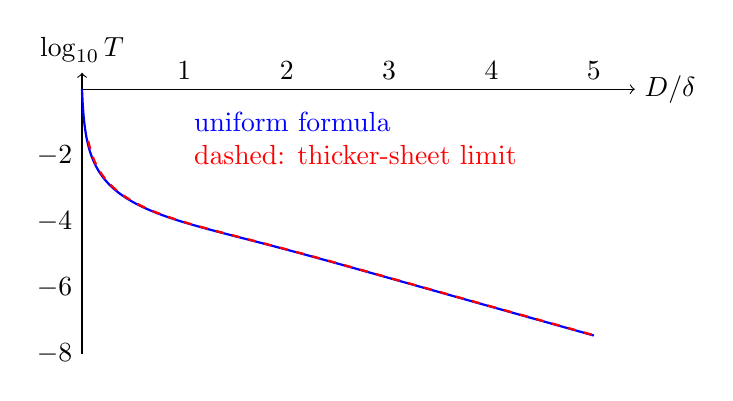
\begin{tikzpicture}[x=1.3cm,y=.42cm]
\draw[->] (0,-8)--(0,.5) node[above] {$\log_{10}T$};\draw[->] (0,0)--(5.4,0) node[right] {$D/\delta$};
\draw[blue,thick] plot coordinates {(0.000000,0.000000) (0.001010,-0.083583) (0.002020,-0.159824) (0.003030,-0.229909) (0.004040,-0.294759) (0.005051,-0.355102) (0.006061,-0.411524) (0.007071,-0.464503) (0.008081,-0.514436) (0.009091,-0.561653) (0.010101,-0.606436) (0.011111,-0.649022) (0.012121,-0.689618) (0.013131,-0.728401) (0.014141,-0.765525) (0.015152,-0.801128) (0.016162,-0.835329) (0.017172,-0.868234) (0.018182,-0.899938) (0.019192,-0.930525) (0.020202,-0.960072) (0.021212,-0.988647) (0.022222,-1.016311) (0.023232,-1.043121) (0.024242,-1.069129) (0.025253,-1.094380) (0.026263,-1.118919) (0.027273,-1.142782) (0.028283,-1.166008) (0.029293,-1.188629) (0.030303,-1.210675) (0.031313,-1.232176) (0.032323,-1.253158) (0.033333,-1.273644) (0.034343,-1.293659) (0.035354,-1.313222) (0.036364,-1.332355) (0.037374,-1.351075) (0.038384,-1.369401) (0.039394,-1.387347) (0.040404,-1.404931) (0.041414,-1.422165) (0.042424,-1.439064) (0.043434,-1.455641) (0.044444,-1.471907) (0.045455,-1.487874) (0.046465,-1.503553) (0.047475,-1.518954) (0.048485,-1.534087) (0.049495,-1.548960) (0.050505,-1.563583) (0.051515,-1.577964) (0.052525,-1.592111) (0.053535,-1.606031) (0.054545,-1.619732) (0.055556,-1.633219) (0.056566,-1.646501) (0.057576,-1.659582) (0.058586,-1.672470) (0.059596,-1.685168) (0.060606,-1.697684) (0.061616,-1.710023) (0.062626,-1.722188) (0.063636,-1.734185) (0.064646,-1.746019) (0.065657,-1.757694) (0.066667,-1.769214) (0.067677,-1.780583) (0.068687,-1.791805) (0.069697,-1.802884) (0.070707,-1.813824) (0.071717,-1.824627) (0.072727,-1.835298) (0.073737,-1.845840) (0.074747,-1.856255) (0.075758,-1.866546) (0.076768,-1.876717) (0.077778,-1.886770) (0.078788,-1.896709) (0.079798,-1.906534) (0.080808,-1.916250) (0.081818,-1.925859) (0.082828,-1.935362) (0.083838,-1.944763) (0.084848,-1.954062) (0.085859,-1.963264) (0.086869,-1.972368) (0.087879,-1.981379) (0.088889,-1.990297) (0.089899,-1.999124) (0.090909,-2.007863) (0.091919,-2.016514) (0.092929,-2.025080) (0.093939,-2.033563) (0.094949,-2.041963) (0.095960,-2.050283) (0.096970,-2.058524) (0.097980,-2.066688) (0.098990,-2.074775) (0.100000,-2.082788) (0.119679,-2.225743) (0.139357,-2.348463) (0.159036,-2.455975) (0.178715,-2.551637) (0.198394,-2.637805) (0.218072,-2.716197) (0.237751,-2.788103) (0.257430,-2.854518) (0.277108,-2.916223) (0.296787,-2.973845) (0.316466,-3.027895) (0.336145,-3.078792) (0.355823,-3.126888) (0.375502,-3.172479) (0.395181,-3.215817) (0.414859,-3.257119) (0.434538,-3.296571) (0.454217,-3.334337) (0.473896,-3.370560) (0.493574,-3.405367) (0.513253,-3.438868) (0.532932,-3.471165) (0.552610,-3.502346) (0.572289,-3.532491) (0.591968,-3.561675) (0.611647,-3.589961) (0.631325,-3.617411) (0.651004,-3.644079) (0.670683,-3.670016) (0.690361,-3.695267) (0.710040,-3.719875) (0.729719,-3.743880) (0.749398,-3.767317) (0.769076,-3.790221) (0.788755,-3.812624) (0.808434,-3.834554) (0.828112,-3.856040) (0.847791,-3.877107) (0.867470,-3.897780) (0.887149,-3.918081) (0.906827,-3.938033) (0.926506,-3.957655) (0.946185,-3.976967) (0.965863,-3.995987) (0.985542,-4.014734) (1.005221,-4.033222) (1.024900,-4.051468) (1.044578,-4.069487) (1.064257,-4.087293) (1.083936,-4.104899) (1.103614,-4.122320) (1.123293,-4.139566) (1.142972,-4.156651) (1.162651,-4.173585) (1.182329,-4.190379) (1.202008,-4.207044) (1.221687,-4.223589) (1.241365,-4.240025) (1.261044,-4.256360) (1.280723,-4.272603) (1.300402,-4.288762) (1.320080,-4.304845) (1.339759,-4.320860) (1.359438,-4.336815) (1.379116,-4.352716) (1.398795,-4.368569) (1.418474,-4.384382) (1.438153,-4.400159) (1.457831,-4.415908) (1.477510,-4.431632) (1.497189,-4.447338) (1.516867,-4.463030) (1.536546,-4.478713) (1.556225,-4.494391) (1.575904,-4.510068) (1.595582,-4.525748) (1.615261,-4.541434) (1.634940,-4.557130) (1.654618,-4.572838) (1.674297,-4.588563) (1.693976,-4.604305) (1.713655,-4.620068) (1.733333,-4.635854) (1.753012,-4.651665) (1.772691,-4.667503) (1.792369,-4.683368) (1.812048,-4.699264) (1.831727,-4.715190) (1.851406,-4.731148) (1.871084,-4.747139) (1.890763,-4.763164) (1.910442,-4.779223) (1.930120,-4.795317) (1.949799,-4.811446) (1.969478,-4.827611) (1.989157,-4.843811) (2.008835,-4.860046) (2.028514,-4.876317) (2.048193,-4.892624) (2.067871,-4.908965) (2.087550,-4.925341) (2.107229,-4.941751) (2.126908,-4.958194) (2.146586,-4.974671) (2.166265,-4.991181) (2.185944,-5.007722) (2.205622,-5.024294) (2.225301,-5.040897) (2.244980,-5.057529) (2.264659,-5.074190) (2.284337,-5.090879) (2.304016,-5.107594) (2.323695,-5.124336) (2.343373,-5.141103) (2.363052,-5.157895) (2.382731,-5.174710) (2.402410,-5.191547) (2.422088,-5.208406) (2.441767,-5.225285) (2.461446,-5.242184) (2.481124,-5.259102) (2.500803,-5.276038) (2.520482,-5.292991) (2.540161,-5.309960) (2.559839,-5.326944) (2.579518,-5.343943) (2.599197,-5.360956) (2.618876,-5.377981) (2.638554,-5.395019) (2.658233,-5.412068) (2.677912,-5.429127) (2.697590,-5.446197) (2.717269,-5.463275) (2.736948,-5.480362) (2.756627,-5.497458) (2.776305,-5.514560) (2.795984,-5.531670) (2.815663,-5.548785) (2.835341,-5.565906) (2.855020,-5.583033) (2.874699,-5.600163) (2.894378,-5.617299) (2.914056,-5.634437) (2.933735,-5.651580) (2.953414,-5.668725) (2.973092,-5.685872) (2.992771,-5.703022) (3.012450,-5.720173) (3.032129,-5.737327) (3.051807,-5.754481) (3.071486,-5.771636) (3.091165,-5.788792) (3.110843,-5.805949) (3.130522,-5.823105) (3.150201,-5.840262) (3.169880,-5.857418) (3.189558,-5.874574) (3.209237,-5.891730) (3.228916,-5.908885) (3.248594,-5.926039) (3.268273,-5.943192) (3.287952,-5.960344) (3.307631,-5.977495) (3.327309,-5.994645) (3.346988,-6.011794) (3.366667,-6.028941) (3.386345,-6.046087) (3.406024,-6.063231) (3.425703,-6.080373) (3.445382,-6.097515) (3.465060,-6.114654) (3.484739,-6.131792) (3.504418,-6.148928) (3.524096,-6.166063) (3.543775,-6.183196) (3.563454,-6.200328) (3.583133,-6.217458) (3.602811,-6.234586) (3.622490,-6.251713) (3.642169,-6.268838) (3.661847,-6.285961) (3.681526,-6.303083) (3.701205,-6.320204) (3.720884,-6.337323) (3.740562,-6.354441) (3.760241,-6.371557) (3.779920,-6.388672) (3.799598,-6.405785) (3.819277,-6.422898) (3.838956,-6.440009) (3.858635,-6.457119) (3.878313,-6.474227) (3.897992,-6.491335) (3.917671,-6.508441) (3.937349,-6.525547) (3.957028,-6.542651) (3.976707,-6.559755) (3.996386,-6.576857) (4.016064,-6.593959) (4.035743,-6.611060) (4.055422,-6.628160) (4.075100,-6.645259) (4.094779,-6.662358) (4.114458,-6.679455) (4.134137,-6.696553) (4.153815,-6.713649) (4.173494,-6.730745) (4.193173,-6.747841) (4.212851,-6.764936) (4.232530,-6.782030) (4.252209,-6.799124) (4.271888,-6.816218) (4.291566,-6.833311) (4.311245,-6.850404) (4.330924,-6.867496) (4.350602,-6.884589) (4.370281,-6.901681) (4.389960,-6.918772) (4.409639,-6.935864) (4.429317,-6.952955) (4.448996,-6.970046) (4.468675,-6.987137) (4.488353,-7.004227) (4.508032,-7.021318) (4.527711,-7.038408) (4.547390,-7.055499) (4.567068,-7.072589) (4.586747,-7.089679) (4.606426,-7.106769) (4.626104,-7.123859) (4.645783,-7.140949) (4.665462,-7.158039) (4.685141,-7.175129) (4.704819,-7.192219) (4.724498,-7.209309) (4.744177,-7.226399) (4.763855,-7.243489) (4.783534,-7.260579) (4.803213,-7.277669) (4.822892,-7.294759) (4.842570,-7.311849) (4.862249,-7.328939) (4.881928,-7.346030) (4.901606,-7.363120) (4.921285,-7.380210) (4.940964,-7.397301) (4.960643,-7.414391) (4.980321,-7.431482) (5.000000,-7.448572)};
\draw[red,dashed,thick] plot coordinates {(0.060606,-1.565032) (0.061616,-1.579390) (0.062626,-1.593513) (0.063636,-1.607411) (0.064646,-1.621090) (0.065657,-1.634557) (0.066667,-1.647818) (0.067677,-1.660880) (0.068687,-1.673748) (0.069697,-1.686428) (0.070707,-1.698926) (0.071717,-1.711247) (0.072727,-1.723395) (0.073737,-1.735376) (0.074747,-1.747194) (0.075758,-1.758853) (0.076768,-1.770357) (0.077778,-1.781712) (0.078788,-1.792920) (0.079798,-1.803985) (0.080808,-1.814910) (0.081818,-1.825701) (0.082828,-1.836358) (0.083838,-1.846887) (0.084848,-1.857289) (0.085859,-1.867569) (0.086869,-1.877728) (0.087879,-1.887769) (0.088889,-1.897696) (0.089899,-1.907511) (0.090909,-1.917216) (0.091919,-1.926814) (0.092929,-1.936307) (0.093939,-1.945697) (0.094949,-1.954987) (0.095960,-1.964178) (0.096970,-1.973274) (0.097980,-1.982275) (0.098990,-1.991184) (0.100000,-2.000002) (0.119679,-2.156038) (0.139357,-2.288268) (0.159036,-2.403004) (0.178715,-2.504341) (0.198394,-2.595085) (0.218072,-2.677245) (0.237751,-2.752306) (0.257430,-2.821402) (0.277108,-2.885413) (0.296787,-2.945040) (0.316466,-3.000847) (0.336145,-3.053299) (0.355823,-3.102778) (0.375502,-3.149608) (0.395181,-3.194062) (0.414859,-3.236373) (0.434538,-3.276744) (0.454217,-3.315347) (0.473896,-3.352338) (0.493574,-3.387849) (0.513253,-3.422001) (0.532932,-3.454898) (0.552610,-3.486635) (0.572289,-3.517297) (0.591968,-3.546961) (0.611647,-3.575695) (0.631325,-3.603563) (0.651004,-3.630622) (0.670683,-3.656925) (0.690361,-3.682519) (0.710040,-3.707448) (0.729719,-3.731755) (0.749398,-3.755476) (0.769076,-3.778647) (0.788755,-3.801301) (0.808434,-3.823467) (0.828112,-3.845176) (0.847791,-3.866452) (0.867470,-3.887323) (0.887149,-3.907810) (0.906827,-3.927937) (0.926506,-3.947724) (0.946185,-3.967191) (0.965863,-3.986358) (0.985542,-4.005241) (1.005221,-4.023858) (1.024900,-4.042225) (1.044578,-4.060358) (1.064257,-4.078270) (1.083936,-4.095977) (1.103614,-4.113490) (1.123293,-4.130824) (1.142972,-4.147989) (1.162651,-4.164998) (1.182329,-4.181862) (1.202008,-4.198591) (1.221687,-4.215196) (1.241365,-4.231687) (1.261044,-4.248072) (1.280723,-4.264360) (1.300402,-4.280561) (1.320080,-4.296682) (1.339759,-4.312730) (1.359438,-4.328715) (1.379116,-4.344642) (1.398795,-4.360519) (1.418474,-4.376351) (1.438153,-4.392146) (1.457831,-4.407909) (1.477510,-4.423645) (1.497189,-4.439359) (1.516867,-4.455058) (1.536546,-4.470745) (1.556225,-4.486425) (1.575904,-4.502102) (1.595582,-4.517780) (1.615261,-4.533462) (1.634940,-4.549153) (1.654618,-4.564855) (1.674297,-4.580571) (1.693976,-4.596303) (1.713655,-4.612056) (1.733333,-4.627830) (1.753012,-4.643628) (1.772691,-4.659452) (1.792369,-4.675303) (1.812048,-4.691183) (1.831727,-4.707093) (1.851406,-4.723035) (1.871084,-4.739009) (1.890763,-4.755017) (1.910442,-4.771059) (1.930120,-4.787135) (1.949799,-4.803246) (1.969478,-4.819393) (1.989157,-4.835575) (2.008835,-4.851792) (2.028514,-4.868045) (2.048193,-4.884333) (2.067871,-4.900657) (2.087550,-4.917015) (2.107229,-4.933408) (2.126908,-4.949835) (2.146586,-4.966295) (2.166265,-4.982788) (2.185944,-4.999313) (2.205622,-5.015869) (2.225301,-5.032457) (2.244980,-5.049074) (2.264659,-5.065720) (2.284337,-5.082395) (2.304016,-5.099097) (2.323695,-5.115826) (2.343373,-5.132580) (2.363052,-5.149360) (2.382731,-5.166163) (2.402410,-5.182989) (2.422088,-5.199837) (2.441767,-5.216706) (2.461446,-5.233595) (2.481124,-5.250503) (2.500803,-5.267430) (2.520482,-5.284374) (2.540161,-5.301335) (2.559839,-5.318312) (2.579518,-5.335304) (2.599197,-5.352309) (2.618876,-5.369328) (2.638554,-5.386360) (2.658233,-5.403403) (2.677912,-5.420457) (2.697590,-5.437522) (2.717269,-5.454596) (2.736948,-5.471679) (2.756627,-5.488770) (2.776305,-5.505869) (2.795984,-5.522975) (2.815663,-5.540087) (2.835341,-5.557206) (2.855020,-5.574330) (2.874699,-5.591458) (2.894378,-5.608591) (2.914056,-5.625728) (2.933735,-5.642869) (2.953414,-5.660012) (2.973092,-5.677159) (2.992771,-5.694307) (3.012450,-5.711458) (3.032129,-5.728610) (3.051807,-5.745764) (3.071486,-5.762919) (3.091165,-5.780075) (3.110843,-5.797231) (3.130522,-5.814387) (3.150201,-5.831544) (3.169880,-5.848701) (3.189558,-5.865857) (3.209237,-5.883013) (3.228916,-5.900168) (3.248594,-5.917323) (3.268273,-5.934476) (3.287952,-5.951629) (3.307631,-5.968781) (3.327309,-5.985931) (3.346988,-6.003080) (3.366667,-6.020228) (3.386345,-6.037374) (3.406024,-6.054519) (3.425703,-6.071663) (3.445382,-6.088805) (3.465060,-6.105945) (3.484739,-6.123084) (3.504418,-6.140221) (3.524096,-6.157357) (3.543775,-6.174491) (3.563454,-6.191623) (3.583133,-6.208754) (3.602811,-6.225883) (3.622490,-6.243010) (3.642169,-6.260136) (3.661847,-6.277261) (3.681526,-6.294383) (3.701205,-6.311505) (3.720884,-6.328624) (3.740562,-6.345743) (3.760241,-6.362860) (3.779920,-6.379975) (3.799598,-6.397090) (3.819277,-6.414203) (3.838956,-6.431314) (3.858635,-6.448425) (3.878313,-6.465534) (3.897992,-6.482642) (3.917671,-6.499749) (3.937349,-6.516855) (3.957028,-6.533960) (3.976707,-6.551064) (3.996386,-6.568167) (4.016064,-6.585269) (4.035743,-6.602370) (4.055422,-6.619471) (4.075100,-6.636570) (4.094779,-6.653669) (4.114458,-6.670768) (4.134137,-6.687865) (4.153815,-6.704962) (4.173494,-6.722058) (4.193173,-6.739154) (4.212851,-6.756249) (4.232530,-6.773344) (4.252209,-6.790438) (4.271888,-6.807532) (4.291566,-6.824625) (4.311245,-6.841719) (4.330924,-6.858811) (4.350602,-6.875904) (4.370281,-6.892996) (4.389960,-6.910087) (4.409639,-6.927179) (4.429317,-6.944270) (4.448996,-6.961361) (4.468675,-6.978452) (4.488353,-6.995543) (4.508032,-7.012634) (4.527711,-7.029724) (4.547390,-7.046815) (4.567068,-7.063905) (4.586747,-7.080995) (4.606426,-7.098085) (4.626104,-7.115175) (4.645783,-7.132265) (4.665462,-7.149355) (4.685141,-7.166445) (4.704819,-7.183535) (4.724498,-7.200625) (4.744177,-7.217715) (4.763855,-7.234805) (4.783534,-7.251895) (4.803213,-7.268985) (4.822892,-7.286075) (4.842570,-7.303165) (4.862249,-7.320255) (4.881928,-7.337346) (4.901606,-7.354436) (4.921285,-7.371526) (4.940964,-7.388617) (4.960643,-7.405707) (4.980321,-7.422797) (5.000000,-7.439888)};
\foreach \x in {1,2,3,4,5} \node[above] at (\x,0) {$\x$};
\foreach \y in {-2,-4,-6,-8} \node[left] at (0,\y) {$\y$};
\node[blue,right] at (1,-1) {uniform formula};\node[red,right] at (1,-2) {dashed: thicker-sheet limit};
\end{tikzpicture}

\end{center}

\Needspace{5\baselineskip}
\par\bigskip
\noindent\textbf{7.6}\quad A plane wave of frequency $\omega$ is incident normally from vacuum on a semi-infinite slab of material with a \emph{complex} index of refraction $n(\omega)$ [$n^{2}(\omega)=\epsilon(\omega)/\epsilon_{0}$].
\begin{enumerate}
\item[(a)] Show that the ratio of reflected power to incident power is
\[
R=\left|\frac{1-n(\omega)}{1+n(\omega)}\right|^{2}
\]
while the ratio of power transmitted into the medium to the incident power is
\[
T=\frac{4\,\mathrm{Re}\;n(\omega)}{|1+n(\omega)|^{2}}
\]
\item[(b)] Evaluate $\mathrm{Re}[i\omega(\mathbf{E}\cdot\mathbf{D}^{*}-\mathbf{B}\cdot\mathbf{H}^{*})/2]$ as a function of $(x,y,z)$. Show that this rate of change of energy per unit volume accounts for the relative transmitted power $T$.
\item[(c)] For a conductor, with $n^{2}=1+i(\sigma/\omega\epsilon_{0})$, $\sigma$ real, write out the results of parts a and b in the limit $\epsilon_{0}\omega\ll\sigma$. Express your answer in terms of $\delta$ as much as possible. Calculate $\frac{1}{2}\mathrm{Re}(\mathbf{J}^{*}\cdot\mathbf{E})$ and compare with the result of part b. Do both enter the complex form of Poynting's theorem?
\end{enumerate}
\solution
Take the material in $z>0$, $n=u+iv$ with $u,v\geq0$, and
$k_0=\omega/c$. For $\mathbf E_i=E_i\mathbf e_x$ the transmitted
fields are
\[
\mathbf E=\frac{2E_i}{1+n}\mathbf e_x e^{ik_0nz},\qquad
\mathbf H=\frac n{Z_0}\frac{2E_i}{1+n}\mathbf e_y e^{ik_0nz}.
\]
\textbf{(a)} The same boundary equations $1+r=t$, $1-r=nt$
give $r=(1-n)/(1+n)$ and $t=2/(1+n)$. The averaged incident
flux is $|E_i|^2/(2Z_0)$, while the transmitted flux at the surface
is $u|tE_i|^2/(2Z_0)$. Therefore
\[
\boxed{R=\left|\frac{1-n}{1+n}\right|^2,\qquad
T=\frac{4\operatorname{Re}n}{|1+n|^2}.}
\]
Expansion of the two squared moduli proves $R+T=1$ at the interface.
Here $T$ measures flux entering the material, not the flux surviving
to infinite depth.
\textbf{(b)} The magnetic term $\mathbf B\cdot\mathbf H^*
=\mu_0|\mathbf H|^2$ is real. With
$\epsilon=\epsilon_0n^2$ one finds
\begin{align*}
q(z)&=\operatorname{Re}\frac{i\omega}{2}
       (\mathbf E\cdot\mathbf D^*-\mathbf B\cdot\mathbf H^*)\\
&=\frac\omega2\operatorname{Im}\epsilon\,|\mathbf E|^2
=\boxed{\frac{4\omega\epsilon_0uv|E_i|^2}{|1+n|^2}
                              e^{-2k_0vz}}.
\end{align*}
There is no dependence on $x,y$. The flux at depth $z$ is
$S_z(z)=2u|E_i|^2e^{-2k_0vz}/[Z_0|1+n|^2]$; using
$1/Z_0=\epsilon_0c$ verifies $q=-dS_z/dz$.
For $v>0$, integrating to infinity gives
$\int_0^\infty q\,dz=S_z(0)=T|E_i|^2/(2Z_0)$.
In the lossless case $v=0$, the dissipation vanishes and the entering
flux instead propagates to infinity; it must not be equated to a
vanishing absorption integral.
\textbf{(c)} For a good conductor write $p=k_0\delta\ll1$.
Then
\[
n\simeq\frac{1+i}{p},\quad t\simeq(1-i)p,\quad
R\simeq1-2p,\quad T\simeq2p,
\]
and
\[
\boxed{q(z)\simeq\sigma p^2|E_i|^2e^{-2z/\delta}
                =2\epsilon_0\omega|E_i|^2e^{-2z/\delta}.}
\]
The equality uses $\sigma\delta^2=2/(\mu_0\omega)$.
Ohm's law gives
$\tfrac12\operatorname{Re}(\mathbf J^*\cdot\mathbf E)
=\sigma|\mathbf E|^2/2$, precisely the same heat production.
It enters Poynting's theorem once: either keep an explicit conduction
current with a real background permittivity, or absorb it into
$\epsilon+i\sigma/\omega$. Including both descriptions of the same
current would double-count the loss.

\Needspace{5\baselineskip}
\par\bigskip
\noindent\textbf{7.7}\quad A ribbon beam of plane-polarized radiation of wavelength $\lambda$ is totally reflected internally at a plane boundary between two nonpermeable media with indices of refraction $n$ and $n'$ ($n'<n$). As discussed in Section 7.4, the ratio of the reflected to incident amplitudes is a complex number of modulus unity, $E_{0}''/E_{0}=\exp[i\phi(i,i_{0})]$ for the angle of incidence $i>i_{0}$, where $\sin i_{0}=n'/n$.
\begin{enumerate}
\item[(a)] Show that for a ``monochromatic'' ribbon beam of radiation in the $z$ direction with an electric field amplitude, $E(x)e^{i(kz-\omega t)}$, where $E(x)$ is smooth and finite in transverse extent (but many wavelengths broad), the lowest order approximation in terms of plane waves is
\[
\mathbf{E}(x,z,t)=\boldsymbol{\epsilon}\int d\kappa\;A(\kappa)e^{i\kappa x+ikz-i\omega t}
\]
where $\boldsymbol{\epsilon}$ is a polarization vector, and $A(\kappa)$ is the Fourier transform of $E(x)$, with support in $\kappa$ around $\kappa=0$ small compared to $k$. The finite beam consists of plane waves with a small range of angles of incidence, centered around the geometrical optics value.
\item[(b)] Consider the reflected beam and show that for $i>i_{0}$ the electric field can be expressed approximately as
\[
\mathbf{E}''(x,z,t)=\boldsymbol{\epsilon}''E(x''-\delta x)\,\exp[i\mathbf{k}''\cdot\mathbf{x}-i\omega t+i\phi(i,i_{0})]
\]
where $\boldsymbol{\epsilon}''$ is a polarization vector, $x''$ is the $x$ coordinate perpendicular to $\mathbf{k}''$, the reflected wave vector, and $\delta x=-(1/k)[d\phi(i,i_{0})/di]$.
\item[(c)] With the Fresnel expressions of Section 7.3 for the phases $\phi(i,i_{0})$ for the two states of plane polarization, show that the lateral displacements of reflected beams with respect to the geometric optics position are
\[
D_{\perp}=\frac{\lambda}{\pi}\frac{\sin i}{(\sin^{2}i-\sin^{2}i_{0})^{1/2}}\qquad\text{and}\qquad
D_{\parallel}=D_{\perp}\cdot\frac{\sin^{2}i_{0}}{[\sin^{2}i-\cos^{2}i\cdot\sin^{2}i_{0}]}
\]
The displacement is known as the \emph{Goos--H\"anchen effect} (op.\ cit.).
\end{enumerate}
\solution
Let $k=2\pi/\lambda$ be the wave number in the incident medium;
$\lambda$ is correspondingly its wavelength.
\textbf{(a)} Define
$A(\kappa)=(2\pi)^{-1}\int E(x)e^{-i\kappa x}\,dx$.
The problem writes the inverse integral without a prefactor, so this
$A$ is Jackson's unitary Fourier amplitude [Eqs.~(7.80)--(7.81),
p.~323] divided by $\sqrt{2\pi}$.
The exact scalar angular spectrum in a homogeneous medium is
\[
\int d\kappa\,A(\kappa)
 e^{i\kappa x+i\sqrt{k^2-\kappa^2}\,z-i\omega t}.
\]
A smooth beam of width $w\gg\lambda$ has its important spectrum
at $|\kappa|\sim1/w\ll k$. Expanding
$\sqrt{k^2-\kappa^2}=k-\kappa^2/(2k)+\cdots$ and keeping the
lowest term gives the expression in the question. The polarization
vector can likewise be replaced by its central value to this order.
The ignored quadratic phase describes diffraction and is small over
propagation distances $|z|\ll k/(\Delta\kappa)^2$.
The angular change of an individual component is
$\Delta i\simeq\kappa/k$.
\textbf{(b)} The reflected spectrum is multiplied by
$e^{i\phi(i+\kappa/k)}$. Linearization of that phase gives
\[
e^{i\phi(i+\kappa/k)}
\simeq e^{i\phi(i)}e^{i\kappa\phi'(i)/k}.
\]
After extracting the central reflected plane-wave phase, its
transverse spectrum is therefore
\[
\int A(\kappa)e^{i\kappa[x''+\phi'(i)/k]}\,d\kappa
=E\bigl(x''+\phi'(i)/k\bigr).
\]
Thus
\[
\boxed{\mathbf E''\simeq\boldsymbol\epsilon''E(x''-\delta x)
 e^{i\mathbf k''\cdot\mathbf x-i\omega t+i\phi(i)},\qquad
\delta x=-\frac1k\frac{d\phi}{di}.}
\]
This approximation requires the reflection phase to be approximately
linear over the beam's angular spread.
\textbf{(c)} Put $m=n'/n=\sin i_0$,
$h=\sqrt{\sin^2i-m^2}$, and $c_i=\cos i$.
The two total-reflection phase factors, up to constant phases
irrelevant to the shift, are
\[
r_\perp=\frac{c_i-ih}{c_i+ih},\qquad
r_\parallel=\frac{m^2c_i-ih}{m^2c_i+ih}.
\]
Hence $\phi_\perp=-2\tan^{-1}(h/c_i)$ and
$\phi_\parallel=-2\tan^{-1}[h/(m^2c_i)]$.
Since $h'=\sin i\cos i/h$ and $h^2+c_i^2=1-m^2$,
\[
\phi_\perp'=-\frac{2\sin i}{h},\qquad
\frac{\phi_\parallel'}{\phi_\perp'}
=\frac{m^2(1-m^2)}{h^2+m^4c_i^2}
=\frac{m^2}{\sin^2i-m^2\cos^2i}.
\]
Substitution in part (b) gives the stated transverse displacements:
\[
\boxed{D_\perp=\frac\lambda\pi\frac{\sin i}{\sqrt{\sin^2i-\sin^2i_0}},
\quad D_\parallel=D_\perp
\frac{\sin^2i_0}{\sin^2i-\cos^2i\sin^2i_0}.}
\]
Here $D=\delta x$ is measured perpendicular to the reflected beam.
The corresponding displacement of the beam's footprint \emph{along
the interface} is $D/\cos i$. Close to $i_0$ the formal derivative
diverges, but the linear phase approximation fails when the angular
spread is comparable to $i-i_0$; a finite beam then requires the
unexpanded angular-spectrum integral.

\Needspace{5\baselineskip}
\par\bigskip
\noindent\textbf{7.8}\quad A monochromatic plane wave of frequency $\omega$ is incident normally on a stack of layers of various thicknesses $t_{j}$ and lossless indices of refraction $n_{j}$. Inside the stack, the wave has both forward and backward moving components. The change in the wave through any interface and also from one side of a layer to the other can be described by means of $2\times2$ transfer matrices. If the electric field is written as
\[
E=E_{+}e^{ikx}+E_{-}e^{-ikx}
\]
in each layer, the transfer matrix equation $E'=TE$ is explicitly
\[
\begin{pmatrix}E'_{+}\\ E'_{-}\end{pmatrix}
=\begin{pmatrix}t_{11}&t_{12}\\ t_{21}&t_{22}\end{pmatrix}
\begin{pmatrix}E_{+}\\ E_{-}\end{pmatrix}
\]
\begin{enumerate}
\item[(a)] Show that the transfer matrix for propagation inside, but across, a layer of index of refraction $n_{j}$ and thickness $t_{j}$ is
\[
T_{\mathrm{layer}}(n_{j},t_{j})=
\begin{pmatrix}e^{ik_{j}t_{j}}&0\\ 0&e^{-ik_{j}t_{j}}\end{pmatrix}
=I\cos(k_{j}t_{j})+i\sigma_{3}\sin(k_{j}t_{j})
\]
where $k_{j}=n_{j}\omega/c$, $I$ is the unit matrix, and $\sigma_{k}$ are the Pauli spin matrices of quantum mechanics. Show that the inverse matrix is $T^{*}$.
\item[(b)] Show that the transfer matrix to cross an interface from $n_{1}$ ($x<x_{0}$) to $n_{2}$ ($x>x_{0}$) is
\[
T_{\mathrm{interface}}(2,1)=\frac{1}{2}
\begin{pmatrix}n+1&-(n-1)\\ -(n-1)&n+1\end{pmatrix}
=I\,\frac{(n+1)}{2}-\sigma_{1}\frac{(n-1)}{2}
\]
where $n=n_{1}/n_{2}$.
\item[(c)] Show that for a complete stack, the incident, reflected, and transmitted waves are related by
\[
E_{\mathrm{trans}}=\frac{\det(T)}{t_{22}}\,E_{\mathrm{inc}},\qquad
E_{\mathrm{refl}}=-\frac{t_{21}}{t_{22}}\,E_{\mathrm{inc}}
\]
where $t_{ij}$ are the elements of $T$, the product of the forward-going transfer matrices, including from the material filling space on the incident side into the first layer and from the last layer into the medium filling the space on the transmitted side.
\end{enumerate}
\solution
Amplitudes in a transfer vector are evaluated at a reference plane;
this choice absorbs the local traveling-wave phases at that plane.
If one instead uses fixed global exponential coordinates, the same
relations acquire the corresponding reference-plane phase factors.
\textbf{(a)} Across a uniform thickness $t_j$, the forward wave
acquires $e^{ik_jt_j}$ and the backward wave acquires
$e^{-ik_jt_j}$. Thus
\[
\boxed{T_{\rm layer}=\begin{pmatrix}e^{ik_jt_j}&0\\0&e^{-ik_jt_j}\end{pmatrix}
=I\cos(k_jt_j)+i\sigma_3\sin(k_jt_j).}
\]
Here $\sigma_3=\operatorname{diag}(1,-1)$.
For real $k_jt_j$ its inverse is its componentwise complex
conjugate, since each diagonal factor is then of unit modulus.
\textbf{(b)} At an interface let $n=n_1/n_2$.
Continuity of the tangential electric and magnetic fields gives
\[
E_{2+}+E_{2-}=E_{1+}+E_{1-},\qquad
E_{2+}-E_{2-}=n(E_{1+}-E_{1-}).
\]
Adding and subtracting these equations proves
\[
\boxed{T_{\rm interface}(2,1)=\frac12
 \begin{pmatrix}n+1&1-n\\1-n&n+1\end{pmatrix}
=\frac{n+1}{2}I-\frac{n-1}{2}\sigma_1.}
\]
Its determinant is $n$, and its inverse is the interface matrix with
$1$ and $2$ interchanged.
\textbf{(c)} Multiply matrices in the order encountered, the first
one acting being on the right. With no wave incident from the
transmitted side,
\[
\begin{pmatrix}E_{\rm trans}\\0\end{pmatrix}
=\begin{pmatrix}t_{11}&t_{12}\\t_{21}&t_{22}\end{pmatrix}
 \begin{pmatrix}E_{\rm inc}\\E_{\rm refl}\end{pmatrix}.
\]
The second row gives $E_{\rm refl}=-t_{21}E_{\rm inc}/t_{22}$.
Inserting it in the first row gives
\[
\boxed{E_{\rm trans}=\frac{t_{11}t_{22}-t_{12}t_{21}}{t_{22}}E_{\rm inc}
=\frac{\det T}{t_{22}}E_{\rm inc},\qquad
E_{\rm refl}=-\frac{t_{21}}{t_{22}}E_{\rm inc}.}
\]
The layer determinants are one and the interface determinants
 telescope, so $\det T=n_{\rm inc}/n_{\rm out}$.
Flux conservation provides an independent check:
$T^\dagger\sigma_3T=(n_{\rm inc}/n_{\rm out})\sigma_3$.
Consequently the amplitudes above obey
$|r|^2+(n_{\rm out}/n_{\rm inc})|t|^2=1$ for a lossless stack.

\Needspace{5\baselineskip}
\par\bigskip
\noindent\textbf{7.9}\quad A stack of optical elements consists of $N$ layers with index of refraction $n$ and thickness $t_{1}$, separated by air gaps ($n_{2}=1$) of thickness $t_{2}$. A monochromatic plane wave is incident normally. With appropriate thicknesses, a modest number of layers can cause almost total reflection of a given range of frequencies, even for normal $n$ values (e.g., $1.3<n<1.8$).
\begin{enumerate}
\item[(a)] Show the transfer matrix for the stack is $T_{\mathrm{stack}}=T^{N}(I\cos\alpha_{2}-i\sigma_{3}\sin\alpha_{2})$, where $\alpha_{2}=\omega t_{2}/c$, and the single air gap plus foil transfer matrix is
\begin{align*}
T=(1/4n)\{&[(n+1)^{2}\cos(\alpha_{1}+\alpha_{2})-(n-1)^{2}\cos(\alpha_{1}-\alpha_{2})]I\\
&+i\sigma_{3}[(n+1)^{2}\sin(\alpha_{1}+\alpha_{2})+(n-1)^{2}\sin(\alpha_{1}-\alpha_{2})]\\
&+2\sigma_{1}(n^{2}-1)\sin\alpha_{1}\sin\alpha_{2}\\
&-2\sigma_{2}(n^{2}-1)\sin\alpha_{1}\cos\alpha_{2}\}
\end{align*}
with $\alpha_{1}=n\omega t_{1}/c$.
\item[(b)] If all the layers (both air gaps and foils) have optical thicknesses of a quarter-wavelength of the incident wave, show that
\[
T=-\exp(-\lambda\sigma_{1}),\qquad\text{where }\lambda=\ln(n)
\]
is (roughly) the amplitude ``decay constant'' per layer. Show that the fractional transmitted intensity is
\[
\frac{|E_{\mathrm{trans}}|^{2}}{|E_{\mathrm{inc}}|^{2}}=\mathrm{sech}^{2}[N\ln(n)]=\frac{4n^{2N}}{(n^{2N}+1)^{2}}\to 4\,\exp[-N\ln(n^{2})]
\]
The asymptotic form holds for $n^{2N}\gg1$.
\end{enumerate}
\solution
Let $P_j=I\cos\alpha_j+i\sigma_3\sin\alpha_j$, and write
$I(b,a)$ for the interface matrix from index $a$ to $b$.
A single foil surrounded by air has transfer matrix
\[
F=I(1,n)P_1I(n,1)
=I\cos\alpha_1+iA\sigma_3\sin\alpha_1-B\sigma_2\sin\alpha_1,
\]
where $A=(n^2+1)/(2n)$ and $B=(n^2-1)/(2n)$.
For example, the nontrivial multiplication follows from
\[
I(1,n)\sigma_3I(n,1)=A\sigma_3+iB\sigma_2,
\]
using $\sigma_3\sigma_1=i\sigma_2$,
$\sigma_1\sigma_3=-i\sigma_2$ and
$\sigma_1\sigma_3\sigma_1=-\sigma_3$.
\textbf{(a)} Define the cell to be a gap followed by a foil, so
$T=FP_2$. Then
\[
\begin{aligned}
T={}&(\cos\alpha_1\cos\alpha_2-A\sin\alpha_1\sin\alpha_2)I\\
&+i(\cos\alpha_1\sin\alpha_2+A\sin\alpha_1\cos\alpha_2)\sigma_3\\
&+B\sin\alpha_1\sin\alpha_2\sigma_1
 -B\sin\alpha_1\cos\alpha_2\sigma_2.
\end{aligned}
\]
Product-to-sum identities turn the first two coefficients into
\[
\frac{(n+1)^2\cos(\alpha_1+\alpha_2)
       -(n-1)^2\cos(\alpha_1-\alpha_2)}{4n},
\]
\[
\frac{(n+1)^2\sin(\alpha_1+\alpha_2)
       +(n-1)^2\sin(\alpha_1-\alpha_2)}{4n},
\]
respectively, while the last two are exactly the coefficients
printed in the question. A stack with $N$ foils and $N-1$ gaps is
$F P_2 F P_2\cdots F=(FP_2)^NP_2^{-1}$; hence
\[
\boxed{T_{\rm stack}=T^N(I\cos\alpha_2-i\sigma_3\sin\alpha_2).}
\]
\textbf{(b)} With $\alpha_1=\alpha_2=\pi/2$,
$T=-AI+B\sigma_1$. If $\lambda=\ln n$, then
$A=\cosh\lambda$ and $B=\sinh\lambda$. Since $\sigma_1^2=I$,
\[
\boxed{T=-e^{-\lambda\sigma_1},\quad
T^N=(-1)^N[I\cosh(N\lambda)-\sigma_1\sinh(N\lambda)].}
\]
Multiplication by $P_2^{-1}=-i\sigma_3$ only changes the phases of
its columns. The magnitude of $t_{22}$ for the full stack is
$\cosh(N\lambda)$ and its determinant is one. The incident and
transmitted media are both air, so
\[
\boxed{\frac{|E_{\rm trans}|^2}{|E_{\rm inc}|^2}
=\operatorname{sech}^2(N\ln n)
=\frac{4n^{2N}}{(n^{2N}+1)^2}
\sim4e^{-N\ln(n^2)}.}
\]
Thus the decaying cell eigenvalue has magnitude $e^{-\lambda}$;
intensity transmission decreases exponentially with the number of
quarter-wave foils, with prefactors fixed by the end interfaces.

\Needspace{5\baselineskip}
\par\bigskip
\noindent\textbf{7.10}\quad An arbitrary optical element of length $L$ is placed in a uniform nonabsorbing medium with index of refraction $n(\omega)$ with its front face at $x=0$ and its back face at $x=L$. If a monochromatic plane wave of frequency $\omega$ with amplitude $\psi_{\mathrm{inc}}(\omega,x,t)=\exp[ik(\omega)x-i\omega t]$ is incident on the front face of the element, the transmitted wave amplitude is $\psi_{\mathrm{trans}}(\omega,x,t)=T(\omega)\exp[ik(\omega)(x-L)-i\omega t]$, where the relative transmission amplitude $T(\omega)=\tau(\omega)\exp[i\phi(\omega)]$ is a complex quantity of magnitude $\tau(\omega)$ and phase $\phi(\omega)$.

A plane wave of radiation $\psi_{\mathrm{inc}}(x,t)$, consisting of a coherent superposition of different frequencies centered around $\omega=\omega_{0}$, with support $A(\omega)$ narrow on the scale of variation of $\tau(\omega)$, $\phi(\omega)$ and $k(\omega)$, is incident on the optical element. Show that the transmitted wave for $x>L$ is approximately
\[
\psi_{\mathrm{trans}}(x,t)\approx\tau(\omega_{0})e^{i\beta}\psi_{\mathrm{inc}}(x',t')
\]
where $\beta$ is a constant phase and $x'=x-L$, $t'=t-T$. The transit or group delay time (sometimes attributed in another context to E.~P. Wigner) is $T=[d\phi(\omega)/d\omega]_{\omega=\omega_{0}}$. If $cT<L$, some authors speak of superluminal propagation through the element. Discuss.
\solution
Write the incident packet as
$\psi_{\rm inc}(x,t)=(2\pi)^{-1/2}\int A(\omega)e^{ik(\omega)x-i\omega t}\,d\omega$.
Each frequency is transmitted independently, giving
\[
\psi_{\rm trans}(x,t)=\frac1{\sqrt{2\pi}}\int A(\omega)\tau(\omega)
 e^{i\phi(\omega)+ik(\omega)(x-L)-i\omega t}\,d\omega.
\]
Across its narrow spectrum approximate $\tau(\omega)\simeq\tau_0$
and $\phi(\omega)\simeq\phi_0+T(\omega-\omega_0)$, where
$T=\phi'(\omega_0)$. Combining terms in the exponent then gives
\begin{align*}
\psi_{\rm trans}(x,t)
&\simeq\frac{\tau_0 e^{i(\phi_0-\omega_0T)}}{\sqrt{2\pi}}
 \int A(\omega)e^{ik(\omega)(x-L)-i\omega(t-T)}\,d\omega\\
&=\boxed{\tau_0e^{i\beta}\psi_{\rm inc}(x-L,t-T),\qquad
\beta=\phi_0-\omega_0T.}
\end{align*}
The conditions include
$|\tau'/\tau_0|\Delta\omega\ll1$ and
$|\phi''|(\Delta\omega)^2\ll1$; otherwise the packet is distorted,
and a single translation does not describe it. A linear expansion
of $k(\omega)$ identifies the usual group motion of its envelope in
the surrounding medium, but is not needed for the algebraic shift
relation itself.

The quantity $T$ measures the shift of a narrow-band envelope or
its peak. It is not in general the arrival time of a new signal
front. A frequency-selective element can reshape the leading tail
and thereby advance the transmitted peak, giving $cT<L$ or even
a negative $T$. A sharp front contains frequencies outside this
narrow-band approximation. For a causal electromagnetic material
whose high-frequency index tends to one, the high-frequency
propagator fixes front propagation at no more than $c$, consistently
with the causal response discussed in Section 7.10. Thus $cT<L$
by itself does not establish faster-than-light transport of new
information; the approximation used to infer it cannot describe
the required front.

\Needspace{5\baselineskip}
\par\bigskip
\noindent\textbf{7.11}\quad A simple example of the transit time of the preceding problem is afforded by a slab of lossless dielectric of thickness $d$ and index of refraction $n$ in vacuum.
\begin{enumerate}
\item[(a)] For a plane wave incident normally, show that the magnitude of the transmitted amplitude is
\[
|\tau(\omega)|=\frac{4n}{\sqrt{[(n+1)^{2}-(n-1)^{2}\cos(2z)]^{2}+[(n-1)^{2}\sin(2z)]^{2}}}
\]
while its phase is
\[
\phi(\omega)=z+\arctan\!\left[\frac{(n-1)^{2}\sin(2z)}{(n+1)^{2}-(n-1)^{2}\cos(2z)}\right]
\]
where $z=n\omega d/c$.
\item[(b)] Neglecting dispersion, show that for $z\to0$ and $z=\pi$, $|\tau|=1.0$ and $cT/d=(n^{2}+1)/2$, while for $z=\pi/2$ (quarter-wave plate), $|\tau|=2n/(n^{2}+1)$ and $cT/d=2n^{2}/(n^{2}+1)$. Show also that $cT/d$, averaged \erratum{from $z=0$ to any integer multiple of $\pi/2$}, is $\langle cT/d\rangle=n$. Does this result tell you anything about what you might expect for the observed transit time of a long wave train ($\Delta\omega/\omega\ll1$) through a piece of window glass? Explain.
\item[(c)] Calculate numerically and plot the results as functions of $z$ for the magnitude of the transmission amplitude, its phase, and the transit time in units of $d/c$ for $n=1.5$ and $n=2.0$.
\end{enumerate}
\solution
\textbf{(a)} The two-interface result for a slab in vacuum is
\[
t(\omega)=\frac{4ne^{iz}}{(n+1)^2-(n-1)^2e^{2iz}},\qquad
z=\frac{n\omega d}{c}.
\]
The denominator has real and imaginary parts
$(n+1)^2-(n-1)^2\cos2z$ and $-(n-1)^2\sin2z$.
Taking its modulus and subtracting its phase proves the two
expressions in the question. Its real part is always positive for
$n>0$, so the continuous, unwrapped phase is
\[
\phi=z+\tan^{-1}\frac{(n-1)^2\sin2z}
 {(n+1)^2-(n-1)^2\cos2z}.
\]
It is useful to divide numerator and denominator by $4ne^{iz}$:
\[
t=\frac1{\cos z-iA\sin z},\quad
A=\frac{n^2+1}{2n},\qquad
|t|^2=\frac1{\cos^2z+A^2\sin^2z}.
\]
\textbf{(b)} Differentiation of the argument of
$\cos z+iA\sin z$ gives
\[
\frac{d\phi}{dz}
=\frac{A\cos^2z+A\sin^2z}{\cos^2z+A^2\sin^2z}
=\frac{A}{\cos^2z+A^2\sin^2z}.
\]
For nondispersive $n$, $dz/d\omega=nd/c$, hence
\[
\boxed{\frac{cT}{d}=\frac{nA}{\cos^2z+A^2\sin^2z}=nA|t|^2.}
\]
At $z=0,\pi$, $|t|=1$ and $cT/d=nA=(n^2+1)/2$;
at $z=\pi/2$, $|t|=1/A=2n/(n^2+1)$ and
$cT/d=n/A=2n^2/(n^2+1)$.
On a quarter-wave interval with endpoints at consecutive multiples
of $\pi/2$, substitute $u=\tan z$ (or use symmetry for the next
interval) to find
\[
\int_0^{\pi/2}\frac{A\,dz}{\cos^2z+A^2\sin^2z}
=\int_0^\infty\frac{A\,du}{1+A^2u^2}=\frac\pi2.
\]
Consequently $\langle cT/d\rangle=n$ from $z=0$ to any integer
multiple of $\pi/2$, or over any whole fringe period $\pi$.
An interval of length $\pi/2$ starting at an arbitrary phase need
not have that average; the quarter-wave endpoints matter.

This unweighted average over optical phase is not a universal
measurement of a packet's transit time. A sufficiently narrow
spectrum, $nd\Delta\omega/c\ll1$, samples the delay at its carrier
phase, anywhere between the two limits above. Even a long train
with $\Delta\omega/\omega\ll1$ can cover many fringes in a thick
window because $z\gg1$. In that regime the single-delay approximation
can fail and the separate multiply reflected pulses, coherence,
and detector weighting must be considered. The direct transmitted
pulse travels in time $nd/c$; the displayed average explains that
scale but does not fix every measured peak or energy-centroid delay.
\textbf{(c)} The plotted curves use the exact amplitude, unwrapped
phase, and analytic derivative, not numerical differentiation of a
wrapped arctangent. For $n=1.5$, the amplitude ranges from
$12/13$ to $1$ and $cT/d$ from $18/13$ to $13/8$.
For $n=2$, the ranges are $4/5$ to $1$ and $8/5$ to $5/2$.
The phase increases by $\pi$ over each period of the amplitude.
\begin{center}
% Generated by supplementary/check_ch07.py --write-assets
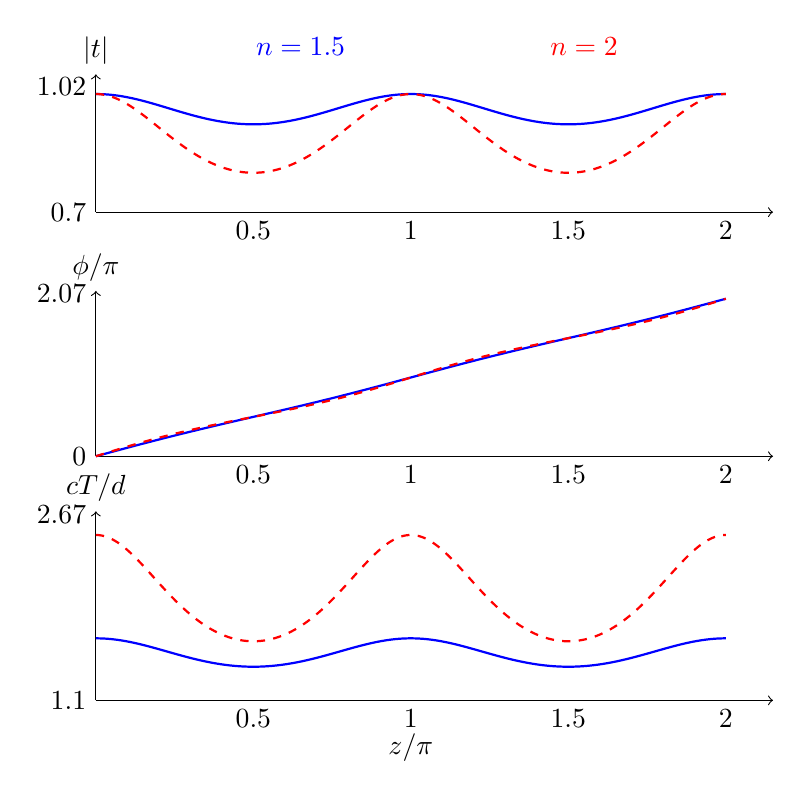
\begin{tikzpicture}[x=4cm]
\begin{scope}[yshift=-3.5cm,y=5cm]
\draw[->] (0,0.7)--(2.15,0.7);\draw[->] (0,0.7)--(0,1.05) node[above] {$|t|$};
\draw[blue,thick] plot coordinates {(0.000000,1.000000) (0.005556,0.999974) (0.011111,0.999894) (0.016667,0.999762) (0.022222,0.999578) (0.027778,0.999341) (0.033333,0.999053) (0.038889,0.998713) (0.044444,0.998323) (0.050000,0.997882) (0.055556,0.997393) (0.061111,0.996854) (0.066667,0.996269) (0.072222,0.995636) (0.077778,0.994958) (0.083333,0.994235) (0.088889,0.993469) (0.094444,0.992661) (0.100000,0.991812) (0.105556,0.990924) (0.111111,0.989998) (0.116667,0.989035) (0.122222,0.988037) (0.127778,0.987005) (0.133333,0.985941) (0.138889,0.984847) (0.144444,0.983725) (0.150000,0.982575) (0.155556,0.981400) (0.161111,0.980201) (0.166667,0.978980) (0.172222,0.977740) (0.177778,0.976480) (0.183333,0.975204) (0.188889,0.973914) (0.194444,0.972610) (0.200000,0.971294) (0.205556,0.969970) (0.211111,0.968637) (0.216667,0.967298) (0.222222,0.965955) (0.227778,0.964609) (0.233333,0.963262) (0.238889,0.961916) (0.244444,0.960573) (0.250000,0.959233) (0.255556,0.957899) (0.261111,0.956572) (0.266667,0.955254) (0.272222,0.953946) (0.277778,0.952649) (0.283333,0.951366) (0.288889,0.950098) (0.294444,0.948845) (0.300000,0.947610) (0.305556,0.946393) (0.311111,0.945197) (0.316667,0.944021) (0.322222,0.942868) (0.327778,0.941739) (0.333333,0.940634) (0.338889,0.939555) (0.344444,0.938503) (0.350000,0.937479) (0.355556,0.936484) (0.361111,0.935518) (0.366667,0.934584) (0.372222,0.933680) (0.377778,0.932810) (0.383333,0.931972) (0.388889,0.931169) (0.394444,0.930400) (0.400000,0.929666) (0.405556,0.928969) (0.411111,0.928308) (0.416667,0.927685) (0.422222,0.927099) (0.427778,0.926551) (0.433333,0.926042) (0.438889,0.925573) (0.444444,0.925143) (0.450000,0.924752) (0.455556,0.924402) (0.461111,0.924093) (0.466667,0.923824) (0.472222,0.923596) (0.477778,0.923409) (0.483333,0.923264) (0.488889,0.923160) (0.494444,0.923098) (0.500000,0.923077) (0.505556,0.923098) (0.511111,0.923160) (0.516667,0.923264) (0.522222,0.923409) (0.527778,0.923596) (0.533333,0.923824) (0.538889,0.924093) (0.544444,0.924402) (0.550000,0.924752) (0.555556,0.925143) (0.561111,0.925573) (0.566667,0.926042) (0.572222,0.926551) (0.577778,0.927099) (0.583333,0.927685) (0.588889,0.928308) (0.594444,0.928969) (0.600000,0.929666) (0.605556,0.930400) (0.611111,0.931169) (0.616667,0.931972) (0.622222,0.932810) (0.627778,0.933680) (0.633333,0.934584) (0.638889,0.935518) (0.644444,0.936484) (0.650000,0.937479) (0.655556,0.938503) (0.661111,0.939555) (0.666667,0.940634) (0.672222,0.941739) (0.677778,0.942868) (0.683333,0.944021) (0.688889,0.945197) (0.694444,0.946393) (0.700000,0.947610) (0.705556,0.948845) (0.711111,0.950098) (0.716667,0.951366) (0.722222,0.952649) (0.727778,0.953946) (0.733333,0.955254) (0.738889,0.956572) (0.744444,0.957899) (0.750000,0.959233) (0.755556,0.960573) (0.761111,0.961916) (0.766667,0.963262) (0.772222,0.964609) (0.777778,0.965955) (0.783333,0.967298) (0.788889,0.968637) (0.794444,0.969970) (0.800000,0.971294) (0.805556,0.972610) (0.811111,0.973914) (0.816667,0.975204) (0.822222,0.976480) (0.827778,0.977740) (0.833333,0.978980) (0.838889,0.980201) (0.844444,0.981400) (0.850000,0.982575) (0.855556,0.983725) (0.861111,0.984847) (0.866667,0.985941) (0.872222,0.987005) (0.877778,0.988037) (0.883333,0.989035) (0.888889,0.989998) (0.894444,0.990924) (0.900000,0.991812) (0.905556,0.992661) (0.911111,0.993469) (0.916667,0.994235) (0.922222,0.994958) (0.927778,0.995636) (0.933333,0.996269) (0.938889,0.996854) (0.944444,0.997393) (0.950000,0.997882) (0.955556,0.998323) (0.961111,0.998713) (0.966667,0.999053) (0.972222,0.999341) (0.977778,0.999578) (0.983333,0.999762) (0.988889,0.999894) (0.994444,0.999974) (1.000000,1.000000) (1.005556,0.999974) (1.011111,0.999894) (1.016667,0.999762) (1.022222,0.999578) (1.027778,0.999341) (1.033333,0.999053) (1.038889,0.998713) (1.044444,0.998323) (1.050000,0.997882) (1.055556,0.997393) (1.061111,0.996854) (1.066667,0.996269) (1.072222,0.995636) (1.077778,0.994958) (1.083333,0.994235) (1.088889,0.993469) (1.094444,0.992661) (1.100000,0.991812) (1.105556,0.990924) (1.111111,0.989998) (1.116667,0.989035) (1.122222,0.988037) (1.127778,0.987005) (1.133333,0.985941) (1.138889,0.984847) (1.144444,0.983725) (1.150000,0.982575) (1.155556,0.981400) (1.161111,0.980201) (1.166667,0.978980) (1.172222,0.977740) (1.177778,0.976480) (1.183333,0.975204) (1.188889,0.973914) (1.194444,0.972610) (1.200000,0.971294) (1.205556,0.969970) (1.211111,0.968637) (1.216667,0.967298) (1.222222,0.965955) (1.227778,0.964609) (1.233333,0.963262) (1.238889,0.961916) (1.244444,0.960573) (1.250000,0.959233) (1.255556,0.957899) (1.261111,0.956572) (1.266667,0.955254) (1.272222,0.953946) (1.277778,0.952649) (1.283333,0.951366) (1.288889,0.950098) (1.294444,0.948845) (1.300000,0.947610) (1.305556,0.946393) (1.311111,0.945197) (1.316667,0.944021) (1.322222,0.942868) (1.327778,0.941739) (1.333333,0.940634) (1.338889,0.939555) (1.344444,0.938503) (1.350000,0.937479) (1.355556,0.936484) (1.361111,0.935518) (1.366667,0.934584) (1.372222,0.933680) (1.377778,0.932810) (1.383333,0.931972) (1.388889,0.931169) (1.394444,0.930400) (1.400000,0.929666) (1.405556,0.928969) (1.411111,0.928308) (1.416667,0.927685) (1.422222,0.927099) (1.427778,0.926551) (1.433333,0.926042) (1.438889,0.925573) (1.444444,0.925143) (1.450000,0.924752) (1.455556,0.924402) (1.461111,0.924093) (1.466667,0.923824) (1.472222,0.923596) (1.477778,0.923409) (1.483333,0.923264) (1.488889,0.923160) (1.494444,0.923098) (1.500000,0.923077) (1.505556,0.923098) (1.511111,0.923160) (1.516667,0.923264) (1.522222,0.923409) (1.527778,0.923596) (1.533333,0.923824) (1.538889,0.924093) (1.544444,0.924402) (1.550000,0.924752) (1.555556,0.925143) (1.561111,0.925573) (1.566667,0.926042) (1.572222,0.926551) (1.577778,0.927099) (1.583333,0.927685) (1.588889,0.928308) (1.594444,0.928969) (1.600000,0.929666) (1.605556,0.930400) (1.611111,0.931169) (1.616667,0.931972) (1.622222,0.932810) (1.627778,0.933680) (1.633333,0.934584) (1.638889,0.935518) (1.644444,0.936484) (1.650000,0.937479) (1.655556,0.938503) (1.661111,0.939555) (1.666667,0.940634) (1.672222,0.941739) (1.677778,0.942868) (1.683333,0.944021) (1.688889,0.945197) (1.694444,0.946393) (1.700000,0.947610) (1.705556,0.948845) (1.711111,0.950098) (1.716667,0.951366) (1.722222,0.952649) (1.727778,0.953946) (1.733333,0.955254) (1.738889,0.956572) (1.744444,0.957899) (1.750000,0.959233) (1.755556,0.960573) (1.761111,0.961916) (1.766667,0.963262) (1.772222,0.964609) (1.777778,0.965955) (1.783333,0.967298) (1.788889,0.968637) (1.794444,0.969970) (1.800000,0.971294) (1.805556,0.972610) (1.811111,0.973914) (1.816667,0.975204) (1.822222,0.976480) (1.827778,0.977740) (1.833333,0.978980) (1.838889,0.980201) (1.844444,0.981400) (1.850000,0.982575) (1.855556,0.983725) (1.861111,0.984847) (1.866667,0.985941) (1.872222,0.987005) (1.877778,0.988037) (1.883333,0.989035) (1.888889,0.989998) (1.894444,0.990924) (1.900000,0.991812) (1.905556,0.992661) (1.911111,0.993469) (1.916667,0.994235) (1.922222,0.994958) (1.927778,0.995636) (1.933333,0.996269) (1.938889,0.996854) (1.944444,0.997393) (1.950000,0.997882) (1.955556,0.998323) (1.961111,0.998713) (1.966667,0.999053) (1.972222,0.999341) (1.977778,0.999578) (1.983333,0.999762) (1.988889,0.999894) (1.994444,0.999974) (2.000000,1.000000)};
\draw[red,dashed,thick] plot coordinates {(0.000000,1.000000) (0.005556,0.999914) (0.011111,0.999658) (0.016667,0.999231) (0.022222,0.998634) (0.027778,0.997870) (0.033333,0.996941) (0.038889,0.995849) (0.044444,0.994597) (0.050000,0.993188) (0.055556,0.991626) (0.061111,0.989915) (0.066667,0.988060) (0.072222,0.986065) (0.077778,0.983935) (0.083333,0.981676) (0.088889,0.979293) (0.094444,0.976792) (0.100000,0.974179) (0.105556,0.971459) (0.111111,0.968639) (0.116667,0.965726) (0.122222,0.962725) (0.127778,0.959643) (0.133333,0.956486) (0.138889,0.953261) (0.144444,0.949973) (0.150000,0.946630) (0.155556,0.943238) (0.161111,0.939802) (0.166667,0.936329) (0.172222,0.932825) (0.177778,0.929295) (0.183333,0.925745) (0.188889,0.922181) (0.194444,0.918608) (0.200000,0.915032) (0.205556,0.911457) (0.211111,0.907888) (0.216667,0.904330) (0.222222,0.900787) (0.227778,0.897264) (0.233333,0.893766) (0.238889,0.890295) (0.244444,0.886856) (0.250000,0.883452) (0.255556,0.880088) (0.261111,0.876765) (0.266667,0.873488) (0.272222,0.870259) (0.277778,0.867081) (0.283333,0.863957) (0.288889,0.860889) (0.294444,0.857880) (0.300000,0.854932) (0.305556,0.852046) (0.311111,0.849226) (0.316667,0.846472) (0.322222,0.843787) (0.327778,0.841171) (0.333333,0.838628) (0.338889,0.836157) (0.344444,0.833761) (0.350000,0.831440) (0.355556,0.829196) (0.361111,0.827030) (0.366667,0.824942) (0.372222,0.822934) (0.377778,0.821007) (0.383333,0.819161) (0.388889,0.817396) (0.394444,0.815714) (0.400000,0.814116) (0.405556,0.812601) (0.411111,0.811170) (0.416667,0.809824) (0.422222,0.808563) (0.427778,0.807388) (0.433333,0.806298) (0.438889,0.805295) (0.444444,0.804378) (0.450000,0.803547) (0.455556,0.802804) (0.461111,0.802147) (0.466667,0.801578) (0.472222,0.801096) (0.477778,0.800702) (0.483333,0.800395) (0.488889,0.800175) (0.494444,0.800044) (0.500000,0.800000) (0.505556,0.800044) (0.511111,0.800175) (0.516667,0.800395) (0.522222,0.800702) (0.527778,0.801096) (0.533333,0.801578) (0.538889,0.802147) (0.544444,0.802804) (0.550000,0.803547) (0.555556,0.804378) (0.561111,0.805295) (0.566667,0.806298) (0.572222,0.807388) (0.577778,0.808563) (0.583333,0.809824) (0.588889,0.811170) (0.594444,0.812601) (0.600000,0.814116) (0.605556,0.815714) (0.611111,0.817396) (0.616667,0.819161) (0.622222,0.821007) (0.627778,0.822934) (0.633333,0.824942) (0.638889,0.827030) (0.644444,0.829196) (0.650000,0.831440) (0.655556,0.833761) (0.661111,0.836157) (0.666667,0.838628) (0.672222,0.841171) (0.677778,0.843787) (0.683333,0.846472) (0.688889,0.849226) (0.694444,0.852046) (0.700000,0.854932) (0.705556,0.857880) (0.711111,0.860889) (0.716667,0.863957) (0.722222,0.867081) (0.727778,0.870259) (0.733333,0.873488) (0.738889,0.876765) (0.744444,0.880088) (0.750000,0.883452) (0.755556,0.886856) (0.761111,0.890295) (0.766667,0.893766) (0.772222,0.897264) (0.777778,0.900787) (0.783333,0.904330) (0.788889,0.907888) (0.794444,0.911457) (0.800000,0.915032) (0.805556,0.918608) (0.811111,0.922181) (0.816667,0.925745) (0.822222,0.929295) (0.827778,0.932825) (0.833333,0.936329) (0.838889,0.939802) (0.844444,0.943238) (0.850000,0.946630) (0.855556,0.949973) (0.861111,0.953261) (0.866667,0.956486) (0.872222,0.959643) (0.877778,0.962725) (0.883333,0.965726) (0.888889,0.968639) (0.894444,0.971459) (0.900000,0.974179) (0.905556,0.976792) (0.911111,0.979293) (0.916667,0.981676) (0.922222,0.983935) (0.927778,0.986065) (0.933333,0.988060) (0.938889,0.989915) (0.944444,0.991626) (0.950000,0.993188) (0.955556,0.994597) (0.961111,0.995849) (0.966667,0.996941) (0.972222,0.997870) (0.977778,0.998634) (0.983333,0.999231) (0.988889,0.999658) (0.994444,0.999914) (1.000000,1.000000) (1.005556,0.999914) (1.011111,0.999658) (1.016667,0.999231) (1.022222,0.998634) (1.027778,0.997870) (1.033333,0.996941) (1.038889,0.995849) (1.044444,0.994597) (1.050000,0.993188) (1.055556,0.991626) (1.061111,0.989915) (1.066667,0.988060) (1.072222,0.986065) (1.077778,0.983935) (1.083333,0.981676) (1.088889,0.979293) (1.094444,0.976792) (1.100000,0.974179) (1.105556,0.971459) (1.111111,0.968639) (1.116667,0.965726) (1.122222,0.962725) (1.127778,0.959643) (1.133333,0.956486) (1.138889,0.953261) (1.144444,0.949973) (1.150000,0.946630) (1.155556,0.943238) (1.161111,0.939802) (1.166667,0.936329) (1.172222,0.932825) (1.177778,0.929295) (1.183333,0.925745) (1.188889,0.922181) (1.194444,0.918608) (1.200000,0.915032) (1.205556,0.911457) (1.211111,0.907888) (1.216667,0.904330) (1.222222,0.900787) (1.227778,0.897264) (1.233333,0.893766) (1.238889,0.890295) (1.244444,0.886856) (1.250000,0.883452) (1.255556,0.880088) (1.261111,0.876765) (1.266667,0.873488) (1.272222,0.870259) (1.277778,0.867081) (1.283333,0.863957) (1.288889,0.860889) (1.294444,0.857880) (1.300000,0.854932) (1.305556,0.852046) (1.311111,0.849226) (1.316667,0.846472) (1.322222,0.843787) (1.327778,0.841171) (1.333333,0.838628) (1.338889,0.836157) (1.344444,0.833761) (1.350000,0.831440) (1.355556,0.829196) (1.361111,0.827030) (1.366667,0.824942) (1.372222,0.822934) (1.377778,0.821007) (1.383333,0.819161) (1.388889,0.817396) (1.394444,0.815714) (1.400000,0.814116) (1.405556,0.812601) (1.411111,0.811170) (1.416667,0.809824) (1.422222,0.808563) (1.427778,0.807388) (1.433333,0.806298) (1.438889,0.805295) (1.444444,0.804378) (1.450000,0.803547) (1.455556,0.802804) (1.461111,0.802147) (1.466667,0.801578) (1.472222,0.801096) (1.477778,0.800702) (1.483333,0.800395) (1.488889,0.800175) (1.494444,0.800044) (1.500000,0.800000) (1.505556,0.800044) (1.511111,0.800175) (1.516667,0.800395) (1.522222,0.800702) (1.527778,0.801096) (1.533333,0.801578) (1.538889,0.802147) (1.544444,0.802804) (1.550000,0.803547) (1.555556,0.804378) (1.561111,0.805295) (1.566667,0.806298) (1.572222,0.807388) (1.577778,0.808563) (1.583333,0.809824) (1.588889,0.811170) (1.594444,0.812601) (1.600000,0.814116) (1.605556,0.815714) (1.611111,0.817396) (1.616667,0.819161) (1.622222,0.821007) (1.627778,0.822934) (1.633333,0.824942) (1.638889,0.827030) (1.644444,0.829196) (1.650000,0.831440) (1.655556,0.833761) (1.661111,0.836157) (1.666667,0.838628) (1.672222,0.841171) (1.677778,0.843787) (1.683333,0.846472) (1.688889,0.849226) (1.694444,0.852046) (1.700000,0.854932) (1.705556,0.857880) (1.711111,0.860889) (1.716667,0.863957) (1.722222,0.867081) (1.727778,0.870259) (1.733333,0.873488) (1.738889,0.876765) (1.744444,0.880088) (1.750000,0.883452) (1.755556,0.886856) (1.761111,0.890295) (1.766667,0.893766) (1.772222,0.897264) (1.777778,0.900787) (1.783333,0.904330) (1.788889,0.907888) (1.794444,0.911457) (1.800000,0.915032) (1.805556,0.918608) (1.811111,0.922181) (1.816667,0.925745) (1.822222,0.929295) (1.827778,0.932825) (1.833333,0.936329) (1.838889,0.939802) (1.844444,0.943238) (1.850000,0.946630) (1.855556,0.949973) (1.861111,0.953261) (1.866667,0.956486) (1.872222,0.959643) (1.877778,0.962725) (1.883333,0.965726) (1.888889,0.968639) (1.894444,0.971459) (1.900000,0.974179) (1.905556,0.976792) (1.911111,0.979293) (1.916667,0.981676) (1.922222,0.983935) (1.927778,0.986065) (1.933333,0.988060) (1.938889,0.989915) (1.944444,0.991626) (1.950000,0.993188) (1.955556,0.994597) (1.961111,0.995849) (1.966667,0.996941) (1.972222,0.997870) (1.977778,0.998634) (1.983333,0.999231) (1.988889,0.999658) (1.994444,0.999914) (2.000000,1.000000)};
\node[left] at (0,0.7) {$0.7$};\node[left] at (0,1.02) {$1.02$};
\node[below] at (0.5,0.7) {$0.5$};
\node[below] at (1,0.7) {$1$};
\node[below] at (1.5,0.7) {$1.5$};
\node[below] at (2,0.7) {$2$};
\node[blue] at (.65,1.12) {$n=1.5$};\node[red] at (1.55,1.12) {$n=2$};
\end{scope}
\begin{scope}[yshift=-3.1cm,y=1cm]
\draw[->] (0,0)--(2.15,0);\draw[->] (0,0)--(0,2.1) node[above] {$\phi/\pi$};
\draw[blue,thick] plot coordinates {(0.000000,0.000000) (0.005556,0.006018) (0.011111,0.012036) (0.016667,0.018053) (0.022222,0.024067) (0.027778,0.030079) (0.033333,0.036088) (0.038889,0.042093) (0.044444,0.048094) (0.050000,0.054090) (0.055556,0.060080) (0.061111,0.066064) (0.066667,0.072041) (0.072222,0.078011) (0.077778,0.083973) (0.083333,0.089927) (0.088889,0.095872) (0.094444,0.101807) (0.100000,0.107733) (0.105556,0.113648) (0.111111,0.119552) (0.116667,0.125445) (0.122222,0.131326) (0.127778,0.137196) (0.133333,0.143053) (0.138889,0.148897) (0.144444,0.154727) (0.150000,0.160545) (0.155556,0.166349) (0.161111,0.172138) (0.166667,0.177914) (0.172222,0.183674) (0.177778,0.189421) (0.183333,0.195152) (0.188889,0.200868) (0.194444,0.206569) (0.200000,0.212255) (0.205556,0.217925) (0.211111,0.223580) (0.216667,0.229219) (0.222222,0.234842) (0.227778,0.240450) (0.233333,0.246042) (0.238889,0.251619) (0.244444,0.257180) (0.250000,0.262726) (0.255556,0.268256) (0.261111,0.273770) (0.266667,0.279270) (0.272222,0.284754) (0.277778,0.290224) (0.283333,0.295679) (0.288889,0.301119) (0.294444,0.306544) (0.300000,0.311956) (0.305556,0.317353) (0.311111,0.322737) (0.316667,0.328107) (0.322222,0.333464) (0.327778,0.338808) (0.333333,0.344140) (0.338889,0.349459) (0.344444,0.354766) (0.350000,0.360061) (0.355556,0.365345) (0.361111,0.370617) (0.366667,0.375879) (0.372222,0.381131) (0.377778,0.386373) (0.383333,0.391605) (0.388889,0.396828) (0.394444,0.402042) (0.400000,0.407248) (0.405556,0.412446) (0.411111,0.417636) (0.416667,0.422819) (0.422222,0.427995) (0.427778,0.433165) (0.433333,0.438329) (0.438889,0.443488) (0.444444,0.448641) (0.450000,0.453790) (0.455556,0.458935) (0.461111,0.464076) (0.466667,0.469214) (0.472222,0.474349) (0.477778,0.479482) (0.483333,0.484613) (0.488889,0.489743) (0.494444,0.494872) (0.500000,0.500000) (0.505556,0.505128) (0.511111,0.510257) (0.516667,0.515387) (0.522222,0.520518) (0.527778,0.525651) (0.533333,0.530786) (0.538889,0.535924) (0.544444,0.541065) (0.550000,0.546210) (0.555556,0.551359) (0.561111,0.556512) (0.566667,0.561671) (0.572222,0.566835) (0.577778,0.572005) (0.583333,0.577181) (0.588889,0.582364) (0.594444,0.587554) (0.600000,0.592752) (0.605556,0.597958) (0.611111,0.603172) (0.616667,0.608395) (0.622222,0.613627) (0.627778,0.618869) (0.633333,0.624121) (0.638889,0.629383) (0.644444,0.634655) (0.650000,0.639939) (0.655556,0.645234) (0.661111,0.650541) (0.666667,0.655860) (0.672222,0.661192) (0.677778,0.666536) (0.683333,0.671893) (0.688889,0.677263) (0.694444,0.682647) (0.700000,0.688044) (0.705556,0.693456) (0.711111,0.698881) (0.716667,0.704321) (0.722222,0.709776) (0.727778,0.715246) (0.733333,0.720730) (0.738889,0.726230) (0.744444,0.731744) (0.750000,0.737274) (0.755556,0.742820) (0.761111,0.748381) (0.766667,0.753958) (0.772222,0.759550) (0.777778,0.765158) (0.783333,0.770781) (0.788889,0.776420) (0.794444,0.782075) (0.800000,0.787745) (0.805556,0.793431) (0.811111,0.799132) (0.816667,0.804848) (0.822222,0.810579) (0.827778,0.816326) (0.833333,0.822086) (0.838889,0.827862) (0.844444,0.833651) (0.850000,0.839455) (0.855556,0.845273) (0.861111,0.851103) (0.866667,0.856947) (0.872222,0.862804) (0.877778,0.868674) (0.883333,0.874555) (0.888889,0.880448) (0.894444,0.886352) (0.900000,0.892267) (0.905556,0.898193) (0.911111,0.904128) (0.916667,0.910073) (0.922222,0.916027) (0.927778,0.921989) (0.933333,0.927959) (0.938889,0.933936) (0.944444,0.939920) (0.950000,0.945910) (0.955556,0.951906) (0.961111,0.957907) (0.966667,0.963912) (0.972222,0.969921) (0.977778,0.975933) (0.983333,0.981947) (0.988889,0.987964) (0.994444,0.993982) (1.000000,1.000000) (1.005556,1.006018) (1.011111,1.012036) (1.016667,1.018053) (1.022222,1.024067) (1.027778,1.030079) (1.033333,1.036088) (1.038889,1.042093) (1.044444,1.048094) (1.050000,1.054090) (1.055556,1.060080) (1.061111,1.066064) (1.066667,1.072041) (1.072222,1.078011) (1.077778,1.083973) (1.083333,1.089927) (1.088889,1.095872) (1.094444,1.101807) (1.100000,1.107733) (1.105556,1.113648) (1.111111,1.119552) (1.116667,1.125445) (1.122222,1.131326) (1.127778,1.137196) (1.133333,1.143053) (1.138889,1.148897) (1.144444,1.154727) (1.150000,1.160545) (1.155556,1.166349) (1.161111,1.172138) (1.166667,1.177914) (1.172222,1.183674) (1.177778,1.189421) (1.183333,1.195152) (1.188889,1.200868) (1.194444,1.206569) (1.200000,1.212255) (1.205556,1.217925) (1.211111,1.223580) (1.216667,1.229219) (1.222222,1.234842) (1.227778,1.240450) (1.233333,1.246042) (1.238889,1.251619) (1.244444,1.257180) (1.250000,1.262726) (1.255556,1.268256) (1.261111,1.273770) (1.266667,1.279270) (1.272222,1.284754) (1.277778,1.290224) (1.283333,1.295679) (1.288889,1.301119) (1.294444,1.306544) (1.300000,1.311956) (1.305556,1.317353) (1.311111,1.322737) (1.316667,1.328107) (1.322222,1.333464) (1.327778,1.338808) (1.333333,1.344140) (1.338889,1.349459) (1.344444,1.354766) (1.350000,1.360061) (1.355556,1.365345) (1.361111,1.370617) (1.366667,1.375879) (1.372222,1.381131) (1.377778,1.386373) (1.383333,1.391605) (1.388889,1.396828) (1.394444,1.402042) (1.400000,1.407248) (1.405556,1.412446) (1.411111,1.417636) (1.416667,1.422819) (1.422222,1.427995) (1.427778,1.433165) (1.433333,1.438329) (1.438889,1.443488) (1.444444,1.448641) (1.450000,1.453790) (1.455556,1.458935) (1.461111,1.464076) (1.466667,1.469214) (1.472222,1.474349) (1.477778,1.479482) (1.483333,1.484613) (1.488889,1.489743) (1.494444,1.494872) (1.500000,1.500000) (1.505556,1.505128) (1.511111,1.510257) (1.516667,1.515387) (1.522222,1.520518) (1.527778,1.525651) (1.533333,1.530786) (1.538889,1.535924) (1.544444,1.541065) (1.550000,1.546210) (1.555556,1.551359) (1.561111,1.556512) (1.566667,1.561671) (1.572222,1.566835) (1.577778,1.572005) (1.583333,1.577181) (1.588889,1.582364) (1.594444,1.587554) (1.600000,1.592752) (1.605556,1.597958) (1.611111,1.603172) (1.616667,1.608395) (1.622222,1.613627) (1.627778,1.618869) (1.633333,1.624121) (1.638889,1.629383) (1.644444,1.634655) (1.650000,1.639939) (1.655556,1.645234) (1.661111,1.650541) (1.666667,1.655860) (1.672222,1.661192) (1.677778,1.666536) (1.683333,1.671893) (1.688889,1.677263) (1.694444,1.682647) (1.700000,1.688044) (1.705556,1.693456) (1.711111,1.698881) (1.716667,1.704321) (1.722222,1.709776) (1.727778,1.715246) (1.733333,1.720730) (1.738889,1.726230) (1.744444,1.731744) (1.750000,1.737274) (1.755556,1.742820) (1.761111,1.748381) (1.766667,1.753958) (1.772222,1.759550) (1.777778,1.765158) (1.783333,1.770781) (1.788889,1.776420) (1.794444,1.782075) (1.800000,1.787745) (1.805556,1.793431) (1.811111,1.799132) (1.816667,1.804848) (1.822222,1.810579) (1.827778,1.816326) (1.833333,1.822086) (1.838889,1.827862) (1.844444,1.833651) (1.850000,1.839455) (1.855556,1.845273) (1.861111,1.851103) (1.866667,1.856947) (1.872222,1.862804) (1.877778,1.868674) (1.883333,1.874555) (1.888889,1.880448) (1.894444,1.886352) (1.900000,1.892267) (1.905556,1.898193) (1.911111,1.904128) (1.916667,1.910073) (1.922222,1.916027) (1.927778,1.921989) (1.933333,1.927959) (1.938889,1.933936) (1.944444,1.939920) (1.950000,1.945910) (1.955556,1.951906) (1.961111,1.957907) (1.966667,1.963912) (1.972222,1.969921) (1.977778,1.975933) (1.983333,1.981947) (1.988889,1.987964) (1.994444,1.993982) (2.000000,2.000000)};
\draw[red,dashed,thick] plot coordinates {(0.000000,0.000000) (0.005556,0.006944) (0.011111,0.013886) (0.016667,0.020823) (0.022222,0.027752) (0.027778,0.034673) (0.033333,0.041581) (0.038889,0.048476) (0.044444,0.055355) (0.050000,0.062215) (0.055556,0.069054) (0.061111,0.075871) (0.066667,0.082664) (0.072222,0.089430) (0.077778,0.096168) (0.083333,0.102875) (0.088889,0.109552) (0.094444,0.116195) (0.100000,0.122803) (0.105556,0.129375) (0.111111,0.135910) (0.116667,0.142406) (0.122222,0.148863) (0.127778,0.155279) (0.133333,0.161653) (0.138889,0.167985) (0.144444,0.174274) (0.150000,0.180519) (0.155556,0.186719) (0.161111,0.192875) (0.166667,0.198986) (0.172222,0.205052) (0.177778,0.211072) (0.183333,0.217046) (0.188889,0.222975) (0.194444,0.228857) (0.200000,0.234695) (0.205556,0.240486) (0.211111,0.246233) (0.216667,0.251935) (0.222222,0.257592) (0.227778,0.263204) (0.233333,0.268773) (0.238889,0.274299) (0.244444,0.279782) (0.250000,0.285223) (0.255556,0.290623) (0.261111,0.295981) (0.266667,0.301300) (0.272222,0.306578) (0.277778,0.311819) (0.283333,0.317021) (0.288889,0.322186) (0.294444,0.327315) (0.300000,0.332408) (0.305556,0.337466) (0.311111,0.342491) (0.316667,0.347483) (0.322222,0.352443) (0.327778,0.357372) (0.333333,0.362271) (0.338889,0.367140) (0.344444,0.371982) (0.350000,0.376796) (0.355556,0.381583) (0.361111,0.386345) (0.366667,0.391083) (0.372222,0.395797) (0.377778,0.400489) (0.383333,0.405160) (0.388889,0.409809) (0.394444,0.414440) (0.400000,0.419051) (0.405556,0.423645) (0.411111,0.428223) (0.416667,0.432784) (0.422222,0.437332) (0.427778,0.441865) (0.433333,0.446386) (0.438889,0.450895) (0.444444,0.455393) (0.450000,0.459882) (0.455556,0.464361) (0.461111,0.468833) (0.466667,0.473298) (0.472222,0.477757) (0.477778,0.482212) (0.483333,0.486662) (0.488889,0.491110) (0.494444,0.495555) (0.500000,0.500000) (0.505556,0.504445) (0.511111,0.508890) (0.516667,0.513338) (0.522222,0.517788) (0.527778,0.522243) (0.533333,0.526702) (0.538889,0.531167) (0.544444,0.535639) (0.550000,0.540118) (0.555556,0.544607) (0.561111,0.549105) (0.566667,0.553614) (0.572222,0.558135) (0.577778,0.562668) (0.583333,0.567216) (0.588889,0.571777) (0.594444,0.576355) (0.600000,0.580949) (0.605556,0.585560) (0.611111,0.590191) (0.616667,0.594840) (0.622222,0.599511) (0.627778,0.604203) (0.633333,0.608917) (0.638889,0.613655) (0.644444,0.618417) (0.650000,0.623204) (0.655556,0.628018) (0.661111,0.632860) (0.666667,0.637729) (0.672222,0.642628) (0.677778,0.647557) (0.683333,0.652517) (0.688889,0.657509) (0.694444,0.662534) (0.700000,0.667592) (0.705556,0.672685) (0.711111,0.677814) (0.716667,0.682979) (0.722222,0.688181) (0.727778,0.693422) (0.733333,0.698700) (0.738889,0.704019) (0.744444,0.709377) (0.750000,0.714777) (0.755556,0.720218) (0.761111,0.725701) (0.766667,0.731227) (0.772222,0.736796) (0.777778,0.742408) (0.783333,0.748065) (0.788889,0.753767) (0.794444,0.759514) (0.800000,0.765305) (0.805556,0.771143) (0.811111,0.777025) (0.816667,0.782954) (0.822222,0.788928) (0.827778,0.794948) (0.833333,0.801014) (0.838889,0.807125) (0.844444,0.813281) (0.850000,0.819481) (0.855556,0.825726) (0.861111,0.832015) (0.866667,0.838347) (0.872222,0.844721) (0.877778,0.851137) (0.883333,0.857594) (0.888889,0.864090) (0.894444,0.870625) (0.900000,0.877197) (0.905556,0.883805) (0.911111,0.890448) (0.916667,0.897125) (0.922222,0.903832) (0.927778,0.910570) (0.933333,0.917336) (0.938889,0.924129) (0.944444,0.930946) (0.950000,0.937785) (0.955556,0.944645) (0.961111,0.951524) (0.966667,0.958419) (0.972222,0.965327) (0.977778,0.972248) (0.983333,0.979177) (0.988889,0.986114) (0.994444,0.993056) (1.000000,1.000000) (1.005556,1.006944) (1.011111,1.013886) (1.016667,1.020823) (1.022222,1.027752) (1.027778,1.034673) (1.033333,1.041581) (1.038889,1.048476) (1.044444,1.055355) (1.050000,1.062215) (1.055556,1.069054) (1.061111,1.075871) (1.066667,1.082664) (1.072222,1.089430) (1.077778,1.096168) (1.083333,1.102875) (1.088889,1.109552) (1.094444,1.116195) (1.100000,1.122803) (1.105556,1.129375) (1.111111,1.135910) (1.116667,1.142406) (1.122222,1.148863) (1.127778,1.155279) (1.133333,1.161653) (1.138889,1.167985) (1.144444,1.174274) (1.150000,1.180519) (1.155556,1.186719) (1.161111,1.192875) (1.166667,1.198986) (1.172222,1.205052) (1.177778,1.211072) (1.183333,1.217046) (1.188889,1.222975) (1.194444,1.228857) (1.200000,1.234695) (1.205556,1.240486) (1.211111,1.246233) (1.216667,1.251935) (1.222222,1.257592) (1.227778,1.263204) (1.233333,1.268773) (1.238889,1.274299) (1.244444,1.279782) (1.250000,1.285223) (1.255556,1.290623) (1.261111,1.295981) (1.266667,1.301300) (1.272222,1.306578) (1.277778,1.311819) (1.283333,1.317021) (1.288889,1.322186) (1.294444,1.327315) (1.300000,1.332408) (1.305556,1.337466) (1.311111,1.342491) (1.316667,1.347483) (1.322222,1.352443) (1.327778,1.357372) (1.333333,1.362271) (1.338889,1.367140) (1.344444,1.371982) (1.350000,1.376796) (1.355556,1.381583) (1.361111,1.386345) (1.366667,1.391083) (1.372222,1.395797) (1.377778,1.400489) (1.383333,1.405160) (1.388889,1.409809) (1.394444,1.414440) (1.400000,1.419051) (1.405556,1.423645) (1.411111,1.428223) (1.416667,1.432784) (1.422222,1.437332) (1.427778,1.441865) (1.433333,1.446386) (1.438889,1.450895) (1.444444,1.455393) (1.450000,1.459882) (1.455556,1.464361) (1.461111,1.468833) (1.466667,1.473298) (1.472222,1.477757) (1.477778,1.482212) (1.483333,1.486662) (1.488889,1.491110) (1.494444,1.495555) (1.500000,1.500000) (1.505556,1.504445) (1.511111,1.508890) (1.516667,1.513338) (1.522222,1.517788) (1.527778,1.522243) (1.533333,1.526702) (1.538889,1.531167) (1.544444,1.535639) (1.550000,1.540118) (1.555556,1.544607) (1.561111,1.549105) (1.566667,1.553614) (1.572222,1.558135) (1.577778,1.562668) (1.583333,1.567216) (1.588889,1.571777) (1.594444,1.576355) (1.600000,1.580949) (1.605556,1.585560) (1.611111,1.590191) (1.616667,1.594840) (1.622222,1.599511) (1.627778,1.604203) (1.633333,1.608917) (1.638889,1.613655) (1.644444,1.618417) (1.650000,1.623204) (1.655556,1.628018) (1.661111,1.632860) (1.666667,1.637729) (1.672222,1.642628) (1.677778,1.647557) (1.683333,1.652517) (1.688889,1.657509) (1.694444,1.662534) (1.700000,1.667592) (1.705556,1.672685) (1.711111,1.677814) (1.716667,1.682979) (1.722222,1.688181) (1.727778,1.693422) (1.733333,1.698700) (1.738889,1.704019) (1.744444,1.709377) (1.750000,1.714777) (1.755556,1.720218) (1.761111,1.725701) (1.766667,1.731227) (1.772222,1.736796) (1.777778,1.742408) (1.783333,1.748065) (1.788889,1.753767) (1.794444,1.759514) (1.800000,1.765305) (1.805556,1.771143) (1.811111,1.777025) (1.816667,1.782954) (1.822222,1.788928) (1.827778,1.794948) (1.833333,1.801014) (1.838889,1.807125) (1.844444,1.813281) (1.850000,1.819481) (1.855556,1.825726) (1.861111,1.832015) (1.866667,1.838347) (1.872222,1.844721) (1.877778,1.851137) (1.883333,1.857594) (1.888889,1.864090) (1.894444,1.870625) (1.900000,1.877197) (1.905556,1.883805) (1.911111,1.890448) (1.916667,1.897125) (1.922222,1.903832) (1.927778,1.910570) (1.933333,1.917336) (1.938889,1.924129) (1.944444,1.930946) (1.950000,1.937785) (1.955556,1.944645) (1.961111,1.951524) (1.966667,1.958419) (1.972222,1.965327) (1.977778,1.972248) (1.983333,1.979177) (1.988889,1.986114) (1.994444,1.993056) (2.000000,2.000000)};
\node[left] at (0,0) {$0$};\node[left] at (0,2.0700000000000003) {$2.07$};
\node[below] at (0.5,0) {$0.5$};
\node[below] at (1,0) {$1$};
\node[below] at (1.5,0) {$1.5$};
\node[below] at (2,0) {$2$};
\end{scope}
\begin{scope}[yshift=-7.8500000000000005cm,y=1.5cm]
\draw[->] (0,1.1)--(2.15,1.1);\draw[->] (0,1.1)--(0,2.7) node[above] {$cT/d$};
\draw[blue,thick] plot coordinates {(0.000000,1.625000) (0.005556,1.624914) (0.011111,1.624656) (0.016667,1.624228) (0.022222,1.623628) (0.027778,1.622860) (0.033333,1.621923) (0.038889,1.620821) (0.044444,1.619554) (0.050000,1.618125) (0.055556,1.616537) (0.061111,1.614793) (0.066667,1.612896) (0.072222,1.610848) (0.077778,1.608655) (0.083333,1.606319) (0.088889,1.603845) (0.094444,1.601237) (0.100000,1.598499) (0.105556,1.595637) (0.111111,1.592655) (0.116667,1.589558) (0.122222,1.586352) (0.127778,1.583041) (0.133333,1.579631) (0.138889,1.576127) (0.144444,1.572536) (0.150000,1.568862) (0.155556,1.565112) (0.161111,1.561291) (0.166667,1.557404) (0.172222,1.553459) (0.177778,1.549460) (0.183333,1.545413) (0.188889,1.541325) (0.194444,1.537201) (0.200000,1.533046) (0.205556,1.528867) (0.211111,1.524669) (0.216667,1.520457) (0.222222,1.516237) (0.227778,1.512015) (0.233333,1.507796) (0.238889,1.503585) (0.244444,1.499387) (0.250000,1.495208) (0.255556,1.491051) (0.261111,1.486923) (0.266667,1.482828) (0.272222,1.478770) (0.277778,1.474753) (0.283333,1.470783) (0.288889,1.466864) (0.294444,1.462999) (0.300000,1.459192) (0.305556,1.455448) (0.311111,1.451770) (0.316667,1.448161) (0.322222,1.444626) (0.327778,1.441167) (0.333333,1.437788) (0.338889,1.434492) (0.344444,1.431281) (0.350000,1.428159) (0.355556,1.425128) (0.361111,1.422191) (0.366667,1.419351) (0.372222,1.416609) (0.377778,1.413968) (0.383333,1.411430) (0.388889,1.408997) (0.394444,1.406672) (0.400000,1.404455) (0.405556,1.402348) (0.411111,1.400354) (0.416667,1.398473) (0.422222,1.396708) (0.427778,1.395058) (0.433333,1.393526) (0.438889,1.392113) (0.444444,1.390819) (0.450000,1.389646) (0.455556,1.388594) (0.461111,1.387664) (0.466667,1.386857) (0.472222,1.386173) (0.477778,1.385613) (0.483333,1.385177) (0.488889,1.384865) (0.494444,1.384678) (0.500000,1.384615) (0.505556,1.384678) (0.511111,1.384865) (0.516667,1.385177) (0.522222,1.385613) (0.527778,1.386173) (0.533333,1.386857) (0.538889,1.387664) (0.544444,1.388594) (0.550000,1.389646) (0.555556,1.390819) (0.561111,1.392113) (0.566667,1.393526) (0.572222,1.395058) (0.577778,1.396708) (0.583333,1.398473) (0.588889,1.400354) (0.594444,1.402348) (0.600000,1.404455) (0.605556,1.406672) (0.611111,1.408997) (0.616667,1.411430) (0.622222,1.413968) (0.627778,1.416609) (0.633333,1.419351) (0.638889,1.422191) (0.644444,1.425128) (0.650000,1.428159) (0.655556,1.431281) (0.661111,1.434492) (0.666667,1.437788) (0.672222,1.441167) (0.677778,1.444626) (0.683333,1.448161) (0.688889,1.451770) (0.694444,1.455448) (0.700000,1.459192) (0.705556,1.462999) (0.711111,1.466864) (0.716667,1.470783) (0.722222,1.474753) (0.727778,1.478770) (0.733333,1.482828) (0.738889,1.486923) (0.744444,1.491051) (0.750000,1.495208) (0.755556,1.499387) (0.761111,1.503585) (0.766667,1.507796) (0.772222,1.512015) (0.777778,1.516237) (0.783333,1.520457) (0.788889,1.524669) (0.794444,1.528867) (0.800000,1.533046) (0.805556,1.537201) (0.811111,1.541325) (0.816667,1.545413) (0.822222,1.549460) (0.827778,1.553459) (0.833333,1.557404) (0.838889,1.561291) (0.844444,1.565112) (0.850000,1.568862) (0.855556,1.572536) (0.861111,1.576127) (0.866667,1.579631) (0.872222,1.583041) (0.877778,1.586352) (0.883333,1.589558) (0.888889,1.592655) (0.894444,1.595637) (0.900000,1.598499) (0.905556,1.601237) (0.911111,1.603845) (0.916667,1.606319) (0.922222,1.608655) (0.927778,1.610848) (0.933333,1.612896) (0.938889,1.614793) (0.944444,1.616537) (0.950000,1.618125) (0.955556,1.619554) (0.961111,1.620821) (0.966667,1.621923) (0.972222,1.622860) (0.977778,1.623628) (0.983333,1.624228) (0.988889,1.624656) (0.994444,1.624914) (1.000000,1.625000) (1.005556,1.624914) (1.011111,1.624656) (1.016667,1.624228) (1.022222,1.623628) (1.027778,1.622860) (1.033333,1.621923) (1.038889,1.620821) (1.044444,1.619554) (1.050000,1.618125) (1.055556,1.616537) (1.061111,1.614793) (1.066667,1.612896) (1.072222,1.610848) (1.077778,1.608655) (1.083333,1.606319) (1.088889,1.603845) (1.094444,1.601237) (1.100000,1.598499) (1.105556,1.595637) (1.111111,1.592655) (1.116667,1.589558) (1.122222,1.586352) (1.127778,1.583041) (1.133333,1.579631) (1.138889,1.576127) (1.144444,1.572536) (1.150000,1.568862) (1.155556,1.565112) (1.161111,1.561291) (1.166667,1.557404) (1.172222,1.553459) (1.177778,1.549460) (1.183333,1.545413) (1.188889,1.541325) (1.194444,1.537201) (1.200000,1.533046) (1.205556,1.528867) (1.211111,1.524669) (1.216667,1.520457) (1.222222,1.516237) (1.227778,1.512015) (1.233333,1.507796) (1.238889,1.503585) (1.244444,1.499387) (1.250000,1.495208) (1.255556,1.491051) (1.261111,1.486923) (1.266667,1.482828) (1.272222,1.478770) (1.277778,1.474753) (1.283333,1.470783) (1.288889,1.466864) (1.294444,1.462999) (1.300000,1.459192) (1.305556,1.455448) (1.311111,1.451770) (1.316667,1.448161) (1.322222,1.444626) (1.327778,1.441167) (1.333333,1.437788) (1.338889,1.434492) (1.344444,1.431281) (1.350000,1.428159) (1.355556,1.425128) (1.361111,1.422191) (1.366667,1.419351) (1.372222,1.416609) (1.377778,1.413968) (1.383333,1.411430) (1.388889,1.408997) (1.394444,1.406672) (1.400000,1.404455) (1.405556,1.402348) (1.411111,1.400354) (1.416667,1.398473) (1.422222,1.396708) (1.427778,1.395058) (1.433333,1.393526) (1.438889,1.392113) (1.444444,1.390819) (1.450000,1.389646) (1.455556,1.388594) (1.461111,1.387664) (1.466667,1.386857) (1.472222,1.386173) (1.477778,1.385613) (1.483333,1.385177) (1.488889,1.384865) (1.494444,1.384678) (1.500000,1.384615) (1.505556,1.384678) (1.511111,1.384865) (1.516667,1.385177) (1.522222,1.385613) (1.527778,1.386173) (1.533333,1.386857) (1.538889,1.387664) (1.544444,1.388594) (1.550000,1.389646) (1.555556,1.390819) (1.561111,1.392113) (1.566667,1.393526) (1.572222,1.395058) (1.577778,1.396708) (1.583333,1.398473) (1.588889,1.400354) (1.594444,1.402348) (1.600000,1.404455) (1.605556,1.406672) (1.611111,1.408997) (1.616667,1.411430) (1.622222,1.413968) (1.627778,1.416609) (1.633333,1.419351) (1.638889,1.422191) (1.644444,1.425128) (1.650000,1.428159) (1.655556,1.431281) (1.661111,1.434492) (1.666667,1.437788) (1.672222,1.441167) (1.677778,1.444626) (1.683333,1.448161) (1.688889,1.451770) (1.694444,1.455448) (1.700000,1.459192) (1.705556,1.462999) (1.711111,1.466864) (1.716667,1.470783) (1.722222,1.474753) (1.727778,1.478770) (1.733333,1.482828) (1.738889,1.486923) (1.744444,1.491051) (1.750000,1.495208) (1.755556,1.499387) (1.761111,1.503585) (1.766667,1.507796) (1.772222,1.512015) (1.777778,1.516237) (1.783333,1.520457) (1.788889,1.524669) (1.794444,1.528867) (1.800000,1.533046) (1.805556,1.537201) (1.811111,1.541325) (1.816667,1.545413) (1.822222,1.549460) (1.827778,1.553459) (1.833333,1.557404) (1.838889,1.561291) (1.844444,1.565112) (1.850000,1.568862) (1.855556,1.572536) (1.861111,1.576127) (1.866667,1.579631) (1.872222,1.583041) (1.877778,1.586352) (1.883333,1.589558) (1.888889,1.592655) (1.894444,1.595637) (1.900000,1.598499) (1.905556,1.601237) (1.911111,1.603845) (1.916667,1.606319) (1.922222,1.608655) (1.927778,1.610848) (1.933333,1.612896) (1.938889,1.614793) (1.944444,1.616537) (1.950000,1.618125) (1.955556,1.619554) (1.961111,1.620821) (1.966667,1.621923) (1.972222,1.622860) (1.977778,1.623628) (1.983333,1.624228) (1.988889,1.624656) (1.994444,1.624914) (2.000000,1.625000)};
\draw[red,dashed,thick] plot coordinates {(0.000000,2.500000) (0.005556,2.499572) (0.011111,2.498288) (0.016667,2.496154) (0.022222,2.493176) (0.027778,2.489363) (0.033333,2.484729) (0.038889,2.479287) (0.044444,2.473056) (0.050000,2.466054) (0.055556,2.458304) (0.061111,2.449829) (0.066667,2.440655) (0.072222,2.430809) (0.077778,2.420321) (0.083333,2.409220) (0.088889,2.397538) (0.094444,2.385307) (0.100000,2.372560) (0.105556,2.359332) (0.111111,2.345656) (0.116667,2.331566) (0.122222,2.317098) (0.127778,2.302286) (0.133333,2.287163) (0.138889,2.271765) (0.144444,2.256124) (0.150000,2.240273) (0.155556,2.224245) (0.161111,2.208071) (0.166667,2.191781) (0.172222,2.175405) (0.177778,2.158973) (0.183333,2.142511) (0.188889,2.126046) (0.194444,2.109603) (0.200000,2.093208) (0.205556,2.076883) (0.211111,2.060650) (0.216667,2.044530) (0.222222,2.028543) (0.227778,2.012708) (0.233333,1.997042) (0.238889,1.981562) (0.244444,1.966283) (0.250000,1.951220) (0.255556,1.936385) (0.261111,1.921792) (0.266667,1.907452) (0.272222,1.893376) (0.277778,1.879574) (0.283333,1.866054) (0.288889,1.852826) (0.294444,1.839895) (0.300000,1.827270) (0.305556,1.814957) (0.311111,1.802961) (0.316667,1.791287) (0.322222,1.779940) (0.327778,1.768924) (0.333333,1.758242) (0.338889,1.747898) (0.344444,1.737894) (0.350000,1.728233) (0.355556,1.718916) (0.361111,1.709947) (0.366667,1.701325) (0.372222,1.693053) (0.377778,1.685131) (0.383333,1.677560) (0.388889,1.670341) (0.394444,1.663475) (0.400000,1.656961) (0.405556,1.650800) (0.411111,1.644993) (0.416667,1.639538) (0.422222,1.634437) (0.427778,1.629688) (0.433333,1.625293) (0.438889,1.621250) (0.444444,1.617559) (0.450000,1.614221) (0.455556,1.611235) (0.461111,1.608601) (0.466667,1.606318) (0.472222,1.604387) (0.477778,1.602808) (0.483333,1.601579) (0.488889,1.600702) (0.494444,1.600175) (0.500000,1.600000) (0.505556,1.600175) (0.511111,1.600702) (0.516667,1.601579) (0.522222,1.602808) (0.527778,1.604387) (0.533333,1.606318) (0.538889,1.608601) (0.544444,1.611235) (0.550000,1.614221) (0.555556,1.617559) (0.561111,1.621250) (0.566667,1.625293) (0.572222,1.629688) (0.577778,1.634437) (0.583333,1.639538) (0.588889,1.644993) (0.594444,1.650800) (0.600000,1.656961) (0.605556,1.663475) (0.611111,1.670341) (0.616667,1.677560) (0.622222,1.685131) (0.627778,1.693053) (0.633333,1.701325) (0.638889,1.709947) (0.644444,1.718916) (0.650000,1.728233) (0.655556,1.737894) (0.661111,1.747898) (0.666667,1.758242) (0.672222,1.768924) (0.677778,1.779940) (0.683333,1.791287) (0.688889,1.802961) (0.694444,1.814957) (0.700000,1.827270) (0.705556,1.839895) (0.711111,1.852826) (0.716667,1.866054) (0.722222,1.879574) (0.727778,1.893376) (0.733333,1.907452) (0.738889,1.921792) (0.744444,1.936385) (0.750000,1.951220) (0.755556,1.966283) (0.761111,1.981562) (0.766667,1.997042) (0.772222,2.012708) (0.777778,2.028543) (0.783333,2.044530) (0.788889,2.060650) (0.794444,2.076883) (0.800000,2.093208) (0.805556,2.109603) (0.811111,2.126046) (0.816667,2.142511) (0.822222,2.158973) (0.827778,2.175405) (0.833333,2.191781) (0.838889,2.208071) (0.844444,2.224245) (0.850000,2.240273) (0.855556,2.256124) (0.861111,2.271765) (0.866667,2.287163) (0.872222,2.302286) (0.877778,2.317098) (0.883333,2.331566) (0.888889,2.345656) (0.894444,2.359332) (0.900000,2.372560) (0.905556,2.385307) (0.911111,2.397538) (0.916667,2.409220) (0.922222,2.420321) (0.927778,2.430809) (0.933333,2.440655) (0.938889,2.449829) (0.944444,2.458304) (0.950000,2.466054) (0.955556,2.473056) (0.961111,2.479287) (0.966667,2.484729) (0.972222,2.489363) (0.977778,2.493176) (0.983333,2.496154) (0.988889,2.498288) (0.994444,2.499572) (1.000000,2.500000) (1.005556,2.499572) (1.011111,2.498288) (1.016667,2.496154) (1.022222,2.493176) (1.027778,2.489363) (1.033333,2.484729) (1.038889,2.479287) (1.044444,2.473056) (1.050000,2.466054) (1.055556,2.458304) (1.061111,2.449829) (1.066667,2.440655) (1.072222,2.430809) (1.077778,2.420321) (1.083333,2.409220) (1.088889,2.397538) (1.094444,2.385307) (1.100000,2.372560) (1.105556,2.359332) (1.111111,2.345656) (1.116667,2.331566) (1.122222,2.317098) (1.127778,2.302286) (1.133333,2.287163) (1.138889,2.271765) (1.144444,2.256124) (1.150000,2.240273) (1.155556,2.224245) (1.161111,2.208071) (1.166667,2.191781) (1.172222,2.175405) (1.177778,2.158973) (1.183333,2.142511) (1.188889,2.126046) (1.194444,2.109603) (1.200000,2.093208) (1.205556,2.076883) (1.211111,2.060650) (1.216667,2.044530) (1.222222,2.028543) (1.227778,2.012708) (1.233333,1.997042) (1.238889,1.981562) (1.244444,1.966283) (1.250000,1.951220) (1.255556,1.936385) (1.261111,1.921792) (1.266667,1.907452) (1.272222,1.893376) (1.277778,1.879574) (1.283333,1.866054) (1.288889,1.852826) (1.294444,1.839895) (1.300000,1.827270) (1.305556,1.814957) (1.311111,1.802961) (1.316667,1.791287) (1.322222,1.779940) (1.327778,1.768924) (1.333333,1.758242) (1.338889,1.747898) (1.344444,1.737894) (1.350000,1.728233) (1.355556,1.718916) (1.361111,1.709947) (1.366667,1.701325) (1.372222,1.693053) (1.377778,1.685131) (1.383333,1.677560) (1.388889,1.670341) (1.394444,1.663475) (1.400000,1.656961) (1.405556,1.650800) (1.411111,1.644993) (1.416667,1.639538) (1.422222,1.634437) (1.427778,1.629688) (1.433333,1.625293) (1.438889,1.621250) (1.444444,1.617559) (1.450000,1.614221) (1.455556,1.611235) (1.461111,1.608601) (1.466667,1.606318) (1.472222,1.604387) (1.477778,1.602808) (1.483333,1.601579) (1.488889,1.600702) (1.494444,1.600175) (1.500000,1.600000) (1.505556,1.600175) (1.511111,1.600702) (1.516667,1.601579) (1.522222,1.602808) (1.527778,1.604387) (1.533333,1.606318) (1.538889,1.608601) (1.544444,1.611235) (1.550000,1.614221) (1.555556,1.617559) (1.561111,1.621250) (1.566667,1.625293) (1.572222,1.629688) (1.577778,1.634437) (1.583333,1.639538) (1.588889,1.644993) (1.594444,1.650800) (1.600000,1.656961) (1.605556,1.663475) (1.611111,1.670341) (1.616667,1.677560) (1.622222,1.685131) (1.627778,1.693053) (1.633333,1.701325) (1.638889,1.709947) (1.644444,1.718916) (1.650000,1.728233) (1.655556,1.737894) (1.661111,1.747898) (1.666667,1.758242) (1.672222,1.768924) (1.677778,1.779940) (1.683333,1.791287) (1.688889,1.802961) (1.694444,1.814957) (1.700000,1.827270) (1.705556,1.839895) (1.711111,1.852826) (1.716667,1.866054) (1.722222,1.879574) (1.727778,1.893376) (1.733333,1.907452) (1.738889,1.921792) (1.744444,1.936385) (1.750000,1.951220) (1.755556,1.966283) (1.761111,1.981562) (1.766667,1.997042) (1.772222,2.012708) (1.777778,2.028543) (1.783333,2.044530) (1.788889,2.060650) (1.794444,2.076883) (1.800000,2.093208) (1.805556,2.109603) (1.811111,2.126046) (1.816667,2.142511) (1.822222,2.158973) (1.827778,2.175405) (1.833333,2.191781) (1.838889,2.208071) (1.844444,2.224245) (1.850000,2.240273) (1.855556,2.256124) (1.861111,2.271765) (1.866667,2.287163) (1.872222,2.302286) (1.877778,2.317098) (1.883333,2.331566) (1.888889,2.345656) (1.894444,2.359332) (1.900000,2.372560) (1.905556,2.385307) (1.911111,2.397538) (1.916667,2.409220) (1.922222,2.420321) (1.927778,2.430809) (1.933333,2.440655) (1.938889,2.449829) (1.944444,2.458304) (1.950000,2.466054) (1.955556,2.473056) (1.961111,2.479287) (1.966667,2.484729) (1.972222,2.489363) (1.977778,2.493176) (1.983333,2.496154) (1.988889,2.498288) (1.994444,2.499572) (2.000000,2.500000)};
\node[left] at (0,1.1) {$1.1$};\node[left] at (0,2.6700000000000004) {$2.67$};
\node[below] at (0.5,1.1) {$0.5$};
\node[below] at (1,1.1) {$1$};
\node[below] at (1.5,1.1) {$1.5$};
\node[below] at (2,1.1) {$2$};
\node at (1,.7) {$z/\pi$};
\end{scope}
\end{tikzpicture}

\end{center}

\Needspace{5\baselineskip}
\par\bigskip
\noindent\textbf{7.12}\quad The time dependence of electrical disturbances in good conductors is governed by the frequency-dependent conductivity (7.58). Consider longitudinal electric fields in a conductor, using Ohm's law, the continuity equation, and the differential form of Coulomb's law.
\begin{enumerate}
\item[(a)] Show that the time-Fourier-transformed charge density satisfies the equation
\[
[\sigma(\omega)-i\omega\epsilon_{0}]\rho(\mathbf{x},\omega)=0
\]
\item[(b)] Using the representation $\sigma(\omega)=\sigma_{0}/(1-i\omega\tau)$, where $\sigma_{0}=\epsilon_{0}\omega_{p}^{2}\tau$ and $\tau$ is a damping time, show that in the approximation $\omega_{p}\tau\gg1$ any initial disturbance will oscillate with the plasma frequency and decay in amplitude with a decay constant $\lambda=1/2\tau$. Note that if you use $\sigma(\omega)\simeq\sigma(0)=\sigma_{0}$ in part a, you will find no oscillations and extremely rapid damping with the (wrong) decay constant $\lambda_{w}=\sigma_{0}/\epsilon_{0}$.
\end{enumerate}
\emph{Reference}: W.~M. Saslow and G. Wilkinson, \emph{Am. J. Phys.} \textbf{39}, 1244 (1971).
\solution
Use the convention $e^{-i\omega t}$ and take a homogeneous conductor.
\textbf{(a)} The three relevant equations are
\[
-i\omega\rho+\nabla\cdot\mathbf J=0,\qquad
\mathbf J=\sigma(\omega)\mathbf E,\qquad
\nabla\cdot\mathbf E=\rho/\epsilon_0.
\]
Their elimination gives
$[-i\omega+\sigma(\omega)/\epsilon_0]\rho=0$, or
\[
\boxed{[\sigma(\omega)-i\omega\epsilon_0]\rho(\mathbf x,\omega)=0.}
\]
This is the free longitudinal relaxation condition, with no imposed
external charge source. It applies pointwise to each spatial mode.
\textbf{(b)} Substitution of the Drude conductivity and multiplication
by $1-i\omega\tau$ yield
\[
\left(\omega_p^2-\omega^2-\frac{i\omega}{\tau}\right)\rho=0,
\qquad
\omega_\pm=\pm\sqrt{\omega_p^2-\frac{1}{4\tau^2}}-\frac{i}{2\tau}.
\]
Equivalently the time-domain equation is
\[
\ddot\rho+\tau^{-1}\dot\rho+\omega_p^2\rho=0.
\]
Writing $\Omega=\sqrt{\omega_p^2-1/(4\tau^2)}$, its solution for
general initial charge and initial current divergence is
\[
\boxed{\rho(\mathbf x,t)=e^{-t/(2\tau)}
\left[\rho(\mathbf x,0)\cos\Omega t+
\frac{\dot\rho(\mathbf x,0)+\rho(\mathbf x,0)/(2\tau)}{\Omega}
\sin\Omega t\right].}
\]
For $\omega_p\tau\gg1$, $\Omega\simeq\omega_p$ and the amplitude
decay constant is $1/(2\tau)$. In contrast, replacing $\sigma(\omega)$
by its static value before solving gives
$\dot\rho=-(\sigma_0/\epsilon_0)\rho$ and
$\lambda_w=\omega_p^2\tau$. That approximation requires
$|\omega\tau|\ll1$, whereas the actual modes have
$|\omega\tau|\simeq\omega_p\tau\gg1$. Even its predicted decay rate
would give $\lambda_w\tau=(\omega_p\tau)^2\gg1$, outside its own
range of validity.

\Needspace{5\baselineskip}
\par\bigskip
\noindent\textbf{7.13}\quad A stylized model of the ionosphere is a medium described by the dielectric constant (7.59). Consider the earth with such a medium beginning suddenly at a height $h$ and extending to infinity. For waves with polarization both perpendicular to the plane of incidence (from a horizontal antenna) and in the plane of incidence (from a vertical antenna),
\begin{enumerate}
\item[(a)] show from Fresnel's equations for reflection and refraction that for $\omega>\omega_{p}$ there is a range of angles of incidence for which reflection is not total, but for larger angles there is total reflection back toward the earth.
\item[(b)] A radio amateur operating at a wavelength of 21 meters in the early evening finds that she can receive distant stations located more than 1000 km away, but none closer. Assuming that the signals are being reflected from the $F$ layer of the ionosphere at an effective height of 300 km, calculate the electron density. Compare with the known maximum and minimum $F$ layer densities of $\sim2\times10^{12}$ m$^{-3}$ in the daytime and $\sim(2\text{-}4)\times10^{11}$ m$^{-3}$ at night.
\end{enumerate}
\solution
\textbf{(a)} In the collisionless model (7.59),
$n^2=\epsilon/\epsilon_0=1-\omega_p^2/\omega^2$, with $\mu=\mu_0$.
For $\omega>\omega_p$, $0<n<1$. Conservation of the tangential
wave number gives the normal transmitted wave number
\[
k_z'=\frac\omega c q,\qquad
q=\sqrt{n^2-\sin^2i}=\sqrt{\cos^2i-\omega_p^2/\omega^2},
\]
where the branch has $q\geq0$ or $\operatorname{Im}q>0$.
The reflection coefficients, with fixed tangential electric-field
reference directions, have magnitudes given by
\[
r_\perp=\frac{\cos i-q}{\cos i+q},\qquad
r_\parallel=\frac{q-n^2\cos i}{q+n^2\cos i}.
\]
For the parallel wave $Y_1=1/\cos i$ and $Y_2=n^2/q$;
continuity gives $1+r=t$ and $Y_1(1-r)=Y_2t$, hence the displayed
$r_\parallel=(Y_1-Y_2)/(Y_1+Y_2)$.  A reflected polarization vector
opposite to the fixed tangential direction, as in the usual Fresnel
basis, changes its sign but not its magnitude. When $q$ is real there is a transmitted
flux and generally $|r|<1$; for the parallel polarization there is
also a Brewster zero. At
\[
\boxed{\sin i_c=n,\qquad \cos i_c=\omega_p/\omega,}
\]
$q$ vanishes. For $i>i_c$, write $q=i\kappa$ with real
$\kappa>0$. Both Fresnel coefficients are ratios of complex
conjugates, so $|r_\perp|=|r_\parallel|=1$ and the field above the
interface is evanescent. For $\omega\leq\omega_p$ there is no
propagating transmitted wave at any incidence angle.

\textbf{(b)} First use the locally flat-earth approximation. The
shortest one-hop ground range $D=1000\,\mathrm{km}$ corresponds
to the critical ray, so
\[
\tan i_c=\frac{D}{2h}=\frac53,\qquad
\frac{\omega_p}{\omega}=\frac{2h}{\sqrt{D^2+4h^2}}
=\frac3{\sqrt{34}}.
\]
With $\omega=2\pi c/(21\,\mathrm m)$ and
$\omega_p^2=n_e e^2/(\epsilon_0m_e)$,
\[
\boxed{\omega_p=4.6149\times10^7\,\mathrm{s}^{-1},\qquad
n_e=\frac{\epsilon_0m_e}{e^2}
\left(\frac{2\pi c}{21\,\mathrm m}\right)^2\frac9{34}
=6.69\times10^{11}\,\mathrm{m}^{-3}.}
\]
This is below the stated daytime maximum and above the stated
nighttime range, consistent with an intermediate early-evening
value in this simplified model. Both polarizations have the same
critical angle and give the same inferred density.

Earth curvature is a modest systematic correction to this estimate.
If a spherical earth of radius $R_E$ is used, with $D$ the ground
arc length, put $\vartheta=D/(2R_E)$. At the reflection point,
\[
\cos i_c=\frac{h+R_E(1-\cos\vartheta)}
{\sqrt{R_E^2\sin^2\vartheta+[h+R_E(1-\cos\vartheta)]^2}}.
\]
For the explicitly chosen radius $R_E=6370\,\mathrm{km}$ this
becomes $0.53898$ and gives $n_e=7.34\times10^{11}\,\mathrm{m}^{-3}$.
The problem specifies no earth radius; the flat result above is the
usual plane-layer estimate, while this formula states the geometry
needed for a spherical refinement.

\Needspace{5\baselineskip}
\par\bigskip
\noindent\textbf{7.14}\quad A simple model of propagation of radio waves in the earth's atmosphere or ionosphere consists of a flat earth at $z=0$ and a nonuniform medium with $\epsilon=\epsilon(z)$ for $z>0$. Consider the Maxwell equations under the assumption that the fields are independent of $y$ and can be written as functions of $z$ times $e^{i(kx-\omega t)}$.
\begin{enumerate}
\item[(a)] Show that the wave equation governing the propagation for $z>0$ is
\[
\frac{d^{2}F}{dz^{2}}+q^{2}(z)F=0
\]
where
\[
q^{2}(z)=\omega^{2}\mu_{0}\epsilon(z)-k^{2}
\]
and $F=E_{y}$ for \emph{horizontal} polarization, and
\[
q^{2}(z)=\omega^{2}\mu_{0}\epsilon(z)+\frac{1}{2\epsilon}\frac{d^{2}\epsilon}{dz^{2}}-\frac{3}{4\epsilon^{2}}\left(\frac{d\epsilon}{dz}\right)^{2}-k^{2}
\]
with $F=\sqrt{\epsilon/\epsilon_{0}}\;E_{z}$ for \emph{vertical} polarization \erratum{when $k\ne0$. At $k=0$, use a transverse electric component and the horizontal-polarization equation}.
\item[(b)] Use the WKB approximation to treat the propagation of waves directed vertically into the ionosphere ($k=0$), assuming that the dielectric constant is given by (7.59) with a plasma frequency $\omega_{p}(z)$ governed by an electron density like that shown in Fig.~7.11. Verify that the qualitative arguments in Section 7.6 hold, with departures in detail only for $\omega\sim\omega_{p,\max}$.
\item[(c)] Using the WKB results of part b and the concepts of the propagation of a pulse from Section 7.8, define an effective height of the ionosphere $h'(\omega)$ by calculating the time $T$ for a pulse of dominant frequency $\omega$ to travel up and be reflected back ($h'\equiv cT/2$). [The WKB approximation is discussed in most books on quantum mechanics.]
\end{enumerate}
\solution
Assume $\mu=\mu_0$ and use the stated $e^{ikx-i\omega t}$ dependence.
\textbf{(a)} For horizontal polarization, set
$\mathbf E=E_y(z)\mathbf e_y$. Faraday's law gives
$H_x=-E_y'/(i\omega\mu_0)$ and $H_z=kE_y/(\omega\mu_0)$.
The $y$ component of Amp\`ere's law then gives
\[
E_y''+[\omega^2\mu_0\epsilon(z)-k^2]E_y=0.
\]
For vertical polarization set $\mathbf H=H_y(z)\mathbf e_y$.
Amp\`ere's law gives
\[
E_x=\frac{H_y'}{i\omega\epsilon},\qquad
E_z=-\frac{kH_y}{\omega\epsilon}.
\]
Substitution into $E_x'-ikE_z=i\omega\mu_0H_y$ yields
\[
H_y''-\frac{\epsilon'}\epsilon H_y'
+[\omega^2\mu_0\epsilon-k^2]H_y=0.
\]
Put $H_y=\sqrt\epsilon\,F$ and differentiate both factors. The
coefficient of $F'$ cancels, leaving
\[
\boxed{F''+\left[\omega^2\mu_0\epsilon-k^2
+\frac{\epsilon''}{2\epsilon}
-\frac{3\epsilon'^2}{4\epsilon^2}\right]F=0.}
\]
For $k\ne0$, $\sqrt{\epsilon/\epsilon_0}E_z
=-kF/(\omega\sqrt{\epsilon_0})$, so this is precisely the stated
choice of dependent variable up to a constant. At strictly normal
incidence $E_z=0$; that variable cannot describe a nonzero wave.
One should instead choose either transverse electric component,
which obeys the horizontal-polarization equation. This also avoids
a spurious singular description at a zero of $\epsilon$.

\textbf{(b)} At $k=0$ the physical transverse equation has
\[
q^2(z)=\frac{\omega^2-\omega_p^2(z)}{c^2}.
\]
Away from turning points, the WKB solutions in an allowed region are
\[
F(z)\simeq\frac{C_+}{\sqrt{q(z)}}
 e^{i\int^z q(s)\,ds}+
\frac{C_-}{\sqrt{q(z)}}e^{-i\int^z q(s)\,ds},
\qquad |q'|\ll q^2.
\]
In a forbidden region put $q=i\kappa$; the corresponding solutions
are $\kappa^{-1/2}\exp(\pm\int\kappa\,dz)$. For
$\omega<\omega_{p,\max}$, the rising density produces a turning
point $z_t$ with $\omega_p(z_t)=\omega$.  Near a simple turning
point write $q^2(z)\simeq-\alpha(z-z_t)$, with $\alpha>0$, and put
$\xi=\alpha^{1/3}(z-z_t)$.  Then the equation becomes
$F_{\xi\xi}-\xi F=0$.  Its decaying solution $\operatorname{Ai}(\xi)$
has the allowed-side asymptote
\[
\operatorname{Ai}(-X)\sim\frac1{\sqrt\pi X^{1/4}}
\sin\left(\frac23X^{3/2}+\frac\pi4\right),\qquad X>0.
\]
Here $\tfrac23X^{3/2}=\int_z^{z_t}q(s)\,ds$ to the linearized
order.  Writing the sine as two exponentials gives equal
incoming and reflected amplitudes and thus equal flux.  Their
phase ratio at $z=0$ is
$-i\exp[2i\int_0^{z_t}q\,dz]$, which will give the delay in part (c). If the density decreases again
above its maximum there is a second turning point $z_2$; a thick
forbidden layer transmits only a fraction of order
\[
\mathcal T\sim\exp\left[-2\int_{z_t}^{z_2}
 \frac{\sqrt{\omega_p^2(z)-\omega^2}}c\,dz\right].
\]
For $\omega>\omega_{p,\max}$, $q^2$ is positive throughout and a
smooth layer transmits with small WKB reflection. Close to the
maximum the turning points merge, or the minimum positive $q$
becomes too small for the WKB inequality; partial reflection and
transmission then require a uniform turning-point treatment.
These are the qualifications to the reflection/cutoff picture of
Section 7.6. The required slow density variation is part of the WKB
model; a sharp layer would instead require Fresnel matching.

\textbf{(c)} Refer the reflected wave to $z=0$. For an isolated
simple turning point its phase is
\[
\phi_r(\omega)=2\int_0^{z_t(\omega)}q(z,\omega)\,dz-\frac\pi2.
\]
The narrow-band group delay is $T=d\phi_r/d\omega$. Since
$q(z_t,\omega)=0$, differentiating the endpoint gives no term.
Thus
\[
\boxed{T(\omega)=\frac2c\int_0^{z_t(\omega)}
\frac{dz}{\sqrt{1-\omega_p^2(z)/\omega^2}},\qquad
h'(\omega)=\int_0^{z_t(\omega)}
\frac{dz}{\sqrt{1-\omega_p^2(z)/\omega^2}}.}
\]
The virtual height $h'$ exceeds the physical turning height because
the group velocity $c\sqrt{1-\omega_p^2/\omega^2}$ is below $c$.
The square-root singularity is integrable at a simple turning
point. Near a smooth density maximum the growing delay and
coalescing turning points demand the same uniform treatment as in
part (b). A frequency with no appreciable reflected pulse has no
reflection height defined by this prescription.

\Needspace{5\baselineskip}
\par\bigskip
\noindent\textbf{7.15}\quad The partially ionized interstellar medium (mostly hydrogen) responds to optical frequencies as an electronic plasma in a weak magnetic field. The broad-spectrum pulses from a pulsar allow determination of some average properties of the interstellar medium (e.g., mean electron density and mean magnetic field). The treatment of an electronic plasma in a magnetic field of Section 7.6 is pertinent.
\begin{enumerate}
\item[(a)] Ignoring the weak magnetic field and assuming that $\max(\omega_{p})\ll\omega$, show that $c$ times the transit time of a pulse of mean frequency $\omega$ from a pulsar a distance $R$ away is
\[
ct(\omega)\approx R+\frac{e^{2}}{2\epsilon_{0}m_{\mathrm{e}}\omega^{2}}\int n_{\mathrm{e}}(z)\;dz
\]
where $n_{\mathrm{e}}(z)$ is the electron density along the path of the light.
\item[(b)] The presence of the magnetic field causes a rotation of the plane of linear polarization (Faraday effect). Show that to lowest order in the magnetic field, the polarized light from the pulsar has its polarization rotated through an angle $\delta\theta(\omega)$:
\[
\delta\theta(\omega)\approx-\frac{e^{3}}{2\epsilon_{0}cm_{\mathrm{e}}^{2}\omega^{2}}\int n_{\mathrm{e}}(z)B_{\parallel}(z)\;dz
\]
where $B_{\parallel}(z)$ is the component of $\mathbf{B}$ parallel to the path of the light. \erratum{The signed angle here is positive from $\mathbf e_x$ toward $-\mathbf e_y$ in a right-handed basis with $\mathbf e_z$ along propagation; the opposite azimuth convention reverses the sign.}
\item[(c)] Assuming you had an independent measure of the pulsar distance $R$, what observations would you make in order to infer $\langle n_{\mathrm{e}}\rangle$ and $\langle B_{\parallel}\rangle$? What assumptions, if any, about the polarization are necessary?
\end{enumerate}
\solution
Take $z$ along propagation, neglect collisions and ion motion, and
assume the density and magnetic field change slowly on a wavelength.
\textbf{(a)} From $k=c^{-1}\sqrt{\omega^2-\omega_p^2(z)}$,
\[
\frac{dt}{dz}=\frac{\partial k}{\partial\omega}
=\frac1{c\sqrt{1-\omega_p^2(z)/\omega^2}}
=\frac1c\left[1+\frac{\omega_p^2(z)}{2\omega^2}+\cdots\right].
\]
Using $\omega_p^2(z)=n_e(z)e^2/(\epsilon_0m_e)$ and integrating
along the path gives
\[
\boxed{ct(\omega)=R+\frac{e^2}{2\epsilon_0m_e\omega^2}
\int_0^R n_e(z)\,dz+O(\omega^{-4}).}
\]
\textbf{(b)} Choose a right-handed transverse basis
$(\mathbf e_x,\mathbf e_y,\mathbf e_z)$ and define
$\boldsymbol\epsilon_\pm=(\mathbf e_x\pm i\mathbf e_y)/\sqrt2$.
The helicity conventions of (7.67) give, to first order in
$\omega_B=eB_\parallel/m_e$ and leading order in $\omega_p^2/\omega^2$,
\[
n_\pm\simeq1-\frac{\omega_p^2}{2\omega^2}
\mp\frac{\omega_p^2\omega_B}{2\omega^3},\qquad
k_+-k_-=-\frac{\omega_p^2\omega_B}{c\omega^2}.
\]
A wave initially along $\mathbf e_x$ is the equal superposition of
these two helicities. After propagation its Jones vector, apart
from a common phase, is
\[
\mathbf e_x\cos\frac{\phi_+-\phi_-}{2}
-\mathbf e_y\sin\frac{\phi_+-\phi_-}{2},\qquad
\phi_\pm=\int_0^R k_\pm(z)\,dz.
\]
Consequently the angle convention specified in the amended question,
$\delta\theta=(\phi_+-\phi_-)/2$, gives
\[
\boxed{\delta\theta=-\frac{e^3}{2\epsilon_0c m_e^2\omega^2}
\int_0^R n_e(z)B_\parallel(z)\,dz.}
\]
If polarization azimuth is instead measured positively from
$\mathbf e_x$ toward $\mathbf e_y$, its change is
$\delta\psi=-\delta\theta$. Stating the angle convention is essential
for a signed Faraday formula; the magnitude is independent of it.

\textbf{(c)} Measure pulse arrival times in several frequency bands
and fit the coefficient of $\omega^{-2}$. A common unknown emission
time is removed by taking differences of arrival times. The fitted
column density $\mathcal N_e=\int n_e\,dz$ gives
\[
\langle n_e\rangle=\mathcal N_e/R.
\]
Measure the linear-polarization angle in the same bands, unwrap its
$\pi$ ambiguity, and fit its $\omega^{-2}$ coefficient. This gives
$\mathcal R=\int n_e B_\parallel\,dz$, and hence
\[
\boxed{\langle B_\parallel\rangle_{n_e}
=\frac{\mathcal R}{\mathcal N_e}.}
\]
This is an electron-density-weighted magnetic field, not generally
the ordinary length average. Interpreting it as the latter requires
nearly uniform density or an appropriate absence of correlations.
The source must have measurable linear polarization; its intrinsic
angle must be independent of frequency over the band, or otherwise
known well enough to remove its frequency dependence. Similarly,
intrinsic frequency-dependent pulse emission delays must be
negligible or modeled. Foreground contributions other than the
path being inferred, such as the earth's ionosphere, also enter
those fitted columns and must be subtracted or shown negligible.

\Needspace{5\baselineskip}
\par\bigskip
\noindent\textbf{7.16}\quad Plane waves propagate in a homogeneous, nonpermeable, but \emph{anisotropic} dielectric. \erratum{Assume a transparent reciprocal dielectric, with a real symmetric positive tensor $\epsilon_{ij}$.} If coordinate axes are chosen as the principal axes, the components of displacement along these axes are related to the electric-field components by $D_{i}=\epsilon_{i}E_{i}$ ($i=1,2,3$), where $\epsilon_{i}$ are the eigenvalues of the matrix $\epsilon_{ij}$.
\begin{enumerate}
\item[(a)] Show that plane waves with frequency $\omega$ and wave vector $\mathbf{k}$ must satisfy
\[
\mathbf{k}\times(\mathbf{k}\times\mathbf{E})+\mu_{0}\omega^{2}\mathbf{D}=0
\]
\item[(b)] Show that for a given wave vector $\mathbf{k}=k\mathbf{n}$ there are \erratum{two polarization modes, whose phase velocities $v=\omega/k$ may coincide}. Their velocities satisfy the Fresnel equation \erratum{in its denominator-cleared polynomial form; for nonzero denominators this is}
\[
\sum_{i=1}^{3}\frac{n_{i}^{2}}{v^{2}-v_{i}^{2}}=0
\]
where $v_{i}=1/\sqrt{\mu_{0}\epsilon_{i}}$ is called a principal velocity, and $n_{i}$ is the component of $\mathbf{n}$ along the $i$th principal axis.
\item[(c)] Show that $\mathbf{D}_{a}\cdot\mathbf{D}_{b}=0$ \erratum{for distinct phase velocities, and that orthogonal displacements can be chosen in the degenerate case}, where $\mathbf{D}_{a}$, $\mathbf{D}_{b}$ are the displacements associated with the two modes of propagation.
\end{enumerate}
\solution
The real, symmetric, positive dielectric tensor specified in the
amended statement is needed for real principal velocities and the
ordinary orthogonality asserted here. Write
$V=\operatorname{diag}(v_1^2,v_2^2,v_3^2)$, so
$\mathbf E=\mu_0 V\mathbf D$.
\textbf{(a)} The Fourier-space Maxwell equations are
\[
\mathbf k\times\mathbf E=\omega\mathbf B,\qquad
\mathbf k\times\mathbf B=-\mu_0\omega\mathbf D.
\]
Taking one more cross product in the first equation gives
\[
\boxed{\mathbf k\times(\mathbf k\times\mathbf E)
+\mu_0\omega^2\mathbf D=0.}
\]
Its scalar product with $\mathbf k$ gives
$\mathbf n\cdot\mathbf D=0$ for a nonzero frequency.
\textbf{(b)} With $P=I-\mathbf n\mathbf n^{\mathsf T}$, the vector
equation becomes the two-dimensional eigenvalue problem
\[
v^2\mathbf D=PV\mathbf D=PVP\mathbf D,
\qquad \mathbf D\in\mathbf n^\perp.
\]
The restriction of the real symmetric operator $PVP$ to this plane
has two positive eigenvalues, counted with multiplicity. Componentwise,
\[
(v^2-v_i^2)D_i=-n_i S,\qquad S=\mathbf n\cdot V\mathbf D.
\]
If $S\ne0$ and none of the denominators vanish, imposing
$\sum_i n_iD_i=0$ proves the rational Fresnel equation. The form valid
also at exceptional directions is its denominator-cleared quadratic:
\[
\boxed{\sum_{i=1}^3 n_i^2\prod_{j\ne i}(v^2-v_j^2)=0.}
\]
For example, for $\mathbf n=(1,0,0)$ its roots are $v_2^2$ and
$v_3^2$, with displacements along axes 2 and 3. Neither appears as a
root of the unqualified expression $1/(v^2-v_1^2)=0$. This explicit
principal-axis example verifies why the polynomial qualification in
the statement is necessary. Eigenvalues may coincide, for example
in an isotropic material or on an optic axis; ``two different phase
velocities'' is not valid in those cases.
\textbf{(c)} Symmetry of $PVP$ gives
\[
v_a^2\mathbf D_b\cdot\mathbf D_a
=\mathbf D_b\cdot PVP\mathbf D_a
=\mathbf D_a\cdot PVP\mathbf D_b
=v_b^2\mathbf D_a\cdot\mathbf D_b.
\]
Thus $(v_a^2-v_b^2)\mathbf D_a\cdot\mathbf D_b=0$.
For distinct eigenvalues the two displacements are necessarily
orthogonal; at a repeated eigenvalue an orthonormal basis of the
two-dimensional eigenspace may be chosen. The electric fields
need not be orthogonal, since applying $V$ does not in general
preserve angles.

\Needspace{5\baselineskip}
\par\bigskip
\noindent\textbf{7.17}\quad Consider the problem of dispersion and waves in an electronic plasma when a uniform external magnetic induction $\mathbf{B}_{0}$ is present, as in Section 7.6.
\begin{enumerate}
\item[(a)] Show that in general the susceptibility tensor $\chi_{jk}(\omega)$ defined through $D_{j}=\sum_{k}\epsilon_{jk}E_{k}$, and $\epsilon_{jk}=\epsilon_{0}(\delta_{jk}+\chi_{jk})$, is
\[
\chi_{jk}=-\frac{\omega_{p}^{2}}{\omega^{2}(\omega^{2}-\omega_{B}^{2})}\left[\omega^{2}\delta_{jk}-\omega_{B}^{2}b_{j}b_{k}-i\omega\omega_{B}\epsilon_{jkl}b_{l}\right]
\]
where $\mathbf{b}$ is a unit vector in the direction of $\mathbf{B}_{0}$.
\item[(b)] By straightforward diagonalization of the dielectric tensor $\epsilon_{jk}$ or by an airtight argument based on the approach and results of Section 7.6, find the eigenvalues $\epsilon_{j}$, $j=1,2,3$.
\item[(c)] A plane wave ($\omega$, $\mathbf{k}=k\mathbf{n}$) must satisfy the vector equation of Problem 7.16a. Show that in terms of $\chi_{jk}$ the electric field and wave number must satisfy the three homogeneous equations,
\[
(1-\xi)E_{j}+\xi n_{j}(\mathbf{n}\cdot\mathbf{E})+\sum_{k}\chi_{jk}E_{k}=0,\qquad j=1,2,3
\]
where $\xi=(ck/\omega)^{2}$. Keeping only first-order terms in an expansion of $\chi_{jk}$ in powers of $\omega_{B}/\omega$, show that the effective dielectric constant for propagation of the plane wave is
\[
\epsilon_{\pm}/\epsilon_{0}\approx1-\frac{\omega_{p}^{2}}{\omega^{2}}\mp\frac{\omega_{p}^{2}\omega_{B}\mathbf{b}\cdot\mathbf{n}}{\omega^{3}}
\]
for positive and negative helicity waves.
\end{enumerate}
\solution
Let $e>0$ be the magnitude of the electron charge,
$\omega_B=eB_0/m_e$, and $\omega_p^2=n_e e^2/(\epsilon_0m_e)$.
Neglect damping, ion motion, and terms quadratic in the wave fields.
\textbf{(a)} Define the linear operator $C\mathbf a=\mathbf b\times\mathbf a$.
The electron equation $m_e\ddot{\mathbf x}=-e(\mathbf E+
\dot{\mathbf x}\times\mathbf B_0)$ becomes
\[
(\omega^2 I-i\omega\omega_B C)\mathbf x=\frac e{m_e}\mathbf E.
\]
Write $P_\parallel=\mathbf b\mathbf b^{\mathsf T}$ and
$P_\perp=I-P_\parallel$. Since $CP_\parallel=0$ and
$C^2=-P_\perp$, direct multiplication gives
\[
(\omega^2 I-i\omega\omega_BC)^{-1}
=\frac{P_\parallel}{\omega^2}
+\frac{P_\perp+i(\omega_B/\omega)C}{\omega^2-\omega_B^2}.
\]
The polarization is $\mathbf P=-n_e e\mathbf x$, so
\[
\chi=-\omega_p^2\left[
\frac{P_\parallel}{\omega^2}
+\frac{P_\perp+i(\omega_B/\omega)C}{\omega^2-\omega_B^2}\right].
\]
Using $C_{jk}=-\epsilon_{jkl}b_l$ and combining denominators proves
\[
\boxed{\chi_{jk}=-\frac{\omega_p^2}
{\omega^2(\omega^2-\omega_B^2)}
[\omega^2\delta_{jk}-\omega_B^2b_jb_k
-i\omega\omega_B\epsilon_{jkl}b_l].}
\]
\textbf{(b)} The vector $\mathbf b$ has $C$ eigenvalue zero.
In a right-handed basis about $\mathbf b$, the vectors
$\boldsymbol\epsilon_\pm=(\mathbf e_1\pm i\mathbf e_2)/\sqrt2$
have $C$ eigenvalues $\mp i$. The three dielectric eigenvalues are
therefore
\[
\boxed{\frac{\epsilon_\parallel}{\epsilon_0}=1-\frac{\omega_p^2}{\omega^2},
\qquad
\frac{\epsilon_\pm}{\epsilon_0}
=1-\frac{\omega_p^2}{\omega(\omega\mp\omega_B)}.}
\]
These are material eigenvalues; for arbitrary propagation direction
the electromagnetic normal modes also have to satisfy Maxwell's
longitudinal constraint.
\textbf{(c)} Divide the equation in Problem 7.16(a) by
$\omega^2/c^2$ and substitute $\mathbf D=\epsilon_0(I+\chi)\mathbf E$:
\[
\boxed{(1-\xi)E_j+\xi n_j(\mathbf n\cdot\mathbf E)
+\sum_k\chi_{jk}E_k=0,\qquad \xi=(ck/\omega)^2.}
\]
To first order in $\omega_B/\omega$,
\[
\chi=-\frac{\omega_p^2}{\omega^2}I
-i\frac{\omega_p^2\omega_B}{\omega^3}C+O(\omega_B^2).
\]
Project onto the plane perpendicular to $\mathbf n$. In that plane
$P_n C P_n=(\mathbf b\cdot\mathbf n)C_n$, where
$C_n\mathbf a=\mathbf n\times\mathbf a$.
Its circular eigenvectors have eigenvalues $\mp i$, so the two
transverse equations give
\[
\boxed{\xi_\pm\equiv\epsilon_{\rm eff,\pm}/\epsilon_0
=1-\frac{\omega_p^2}{\omega^2}
\mp\frac{\omega_p^2\omega_B(\mathbf b\cdot\mathbf n)}{\omega^3}
+O(\omega_B^2).}
\]
There is in general a longitudinal electric component of first
order in $\omega_B$, fixed by $\mathbf n\cdot\mathbf D=0$.
Its feedback into the transverse eigenvalues starts at second order.
This expansion is not uniform at the unmagnetized plasma resonance
$1-\omega_p^2/\omega^2=0$, where eliminating that longitudinal
component involves a small denominator.

\Needspace{5\baselineskip}
\par\bigskip
\noindent\textbf{7.18}\quad Magnetohydrodynamic waves can occur in a compressible, nonviscous, perfectly conducting fluid in a uniform static magnetic induction $\mathbf{B}_{0}$. If the propagation direction is not parallel or perpendicular to $\mathbf{B}_{0}$, the waves are not separated into purely longitudinal (magnetosonic) or transverse (Alfv\'en) waves. Let the angle between the propagation direction $\mathbf{k}$ and the field $\mathbf{B}_{0}$ be $\theta$.
\begin{enumerate}
\item[(a)] Show that there are three different waves with phase velocities given by
\begin{align*}
u_{1}^{2}&=(v_{A}\cos\theta)^{2}\\
u_{2,3}^{2}&=\tfrac{1}{2}(s^{2}+v_{A}^{2})\pm\tfrac{1}{2}[(s^{2}+v_{A}^{2})^{2}-4s^{2}v_{A}^{2}\cos^{2}\theta]^{1/2}
\end{align*}
where $s$ is the sound velocity in the fluid, and $v_{A}=(B_{0}^{2}/\mu\rho_{0})^{1/2}$ is the Alfv\'en velocity.
\item[(b)] Find the velocity eigenvectors for the three different waves, and prove that the first (Alfv\'en) wave is always transverse, while the other two are neither longitudinal nor transverse.
\item[(c)] Evaluate the phase velocities and eigenvectors of the mixed waves in the approximation that $v_{A}\gg s$. Show that for one wave the only appreciable component of velocity is parallel to the magnetic field, while for the other the only component is perpendicular to the field and in the plane containing $\mathbf{k}$ and $\mathbf{B}_{0}$.
\end{enumerate}
\solution
Let $\mathbf B_0=B_0\mathbf e_z$ and
$\mathbf k=k(\sin\theta,0,\cos\theta)$, with equilibrium density
$\rho_0$ and $\delta p=s^2\delta\rho$. Write all perturbations as
$e^{i\mathbf k\cdot\mathbf x-i\omega t}$.
\textbf{(a)} The linearized continuity, induction, and momentum
equations of ideal MHD are
\begin{align*}
\rho_1&=\frac{\rho_0}{\omega}\mathbf k\cdot\mathbf v,\\
\mathbf B_1&=\frac{(\mathbf k\cdot\mathbf v)\mathbf B_0
-(\mathbf k\cdot\mathbf B_0)\mathbf v}{\omega},\\
-\omega\rho_0\mathbf v&=-\mathbf k s^2\rho_1
+\frac1\mu(\mathbf k\times\mathbf B_1)\times\mathbf B_0.
\end{align*}
Writing $s_\theta=\sin\theta$, $c_\theta=\cos\theta$, the induction
formula has the explicit components
\[
\mathbf B_1=\frac{kB_0}{\omega}
(-c_\theta v_x,-c_\theta v_y,s_\theta v_x).
\]
Since $(\mathbf k\times\mathbf B_1)\times\mathbf B_0
=\mathbf B_1(\mathbf k\cdot\mathbf B_0)
-\mathbf k(\mathbf B_1\cdot\mathbf B_0)$, its components are
\[
-\frac{k^2B_0^2}{\omega}(v_x,c_\theta^2v_y,0).
\]
The pressure force is proportional to
$(s_\theta,0,c_\theta)(s_\theta v_x+c_\theta v_z)$.
Substitute these into the momentum equation, multiply by
$-\omega/(k^2\rho_0)$, and write $u=\omega/k$,
$v_A^2=B_0^2/(\mu\rho_0)$. The result is
\[
u^2\begin{pmatrix}v_x\\v_y\\v_z\end{pmatrix}
=\begin{pmatrix}
v_A^2+s^2\sin^2\theta&0&s^2\sin\theta\cos\theta\\
0&v_A^2\cos^2\theta&0\\
s^2\sin\theta\cos\theta&0&s^2\cos^2\theta
\end{pmatrix}
\begin{pmatrix}v_x\\v_y\\v_z\end{pmatrix}.
\]
The $y$ eigenvalue is $u_1^2=v_A^2\cos^2\theta$.
The $xz$ block has trace $s^2+v_A^2$ and determinant
$s^2v_A^2\cos^2\theta$. Its characteristic equation is
\[
u^4-(s^2+v_A^2)u^2+s^2v_A^2\cos^2\theta=0,
\]
which gives
\[
\boxed{u_{2,3}^2=\frac{s^2+v_A^2}{2}
\pm\frac12\sqrt{(s^2+v_A^2)^2-4s^2v_A^2\cos^2\theta}.}
\]
\textbf{(b)} The Alfv\'en polarization is
$\mathbf v_1\parallel\mathbf e_y\parallel\mathbf B_0\times\mathbf k$,
hence $\mathbf k\cdot\mathbf v_1=0$ and $\rho_1=0$.
For either mixed root, an unnormalized eigenvector is
\[
\boxed{\mathbf v_{2,3}\ \propto\
\bigl(u_{2,3}^2-s^2\cos^2\theta,\ 0,\
s^2\sin\theta\cos\theta\bigr).}
\]
For the generic oblique case in the question, with $s,v_A>0$,
these vectors are nonzero and can be normalized by their Euclidean
lengths. To test a putative longitudinal mode, apply the $xz$ matrix
to $(\sin\theta,\cos\theta)$; the pressure part is parallel to this
vector but the magnetic part is $(v_A^2\sin\theta,0)$, which is not.
For a putative transverse vector $(\cos\theta,-\sin\theta)$, the
pressure part vanishes and the magnetic result
$(v_A^2\cos\theta,0)$ is again not parallel. Thus neither mixed mode
is longitudinal or transverse for $\sin\theta\cos\theta\ne0$.
The excluded parallel/perpendicular directions and vanishing sound
or magnetic speeds supply the familiar special cases.
\textbf{(c)} Put $\eta=s^2/v_A^2\ll1$. Expansion of the quadratic
roots and their eigenvectors gives
\begin{align*}
u_{\rm fast}^2&=v_A^2+s^2\sin^2\theta+O(s^4/v_A^2),&
\mathbf v_{\rm fast}&\propto(1,0,\eta\sin\theta\cos\theta)+O(\eta^2),\\
u_{\rm slow}^2&=s^2\cos^2\theta[1-\eta\sin^2\theta+O(\eta^2)],&
\mathbf v_{\rm slow}&\propto(-\eta\sin\theta\cos\theta,0,1)+O(\eta^2).
\end{align*}
Thus the fast speed is
$v_A[1+\eta\sin^2\theta/2+O(\eta^2)]$ and the slow speed is
$s|\cos\theta|[1-\eta\sin^2\theta/2+O(\eta^2)]$.
The fast fluid motion is predominantly perpendicular to the field
in the $\mathbf k,\mathbf B_0$ plane, and the slow motion is
predominantly parallel to the field, as requested.

\Needspace{5\baselineskip}
\par\bigskip
\noindent\textbf{7.19}\quad An approximately monochromatic plane wave packet in one dimension has the instantaneous form, $u(x,0)=f(x)\,e^{ik_{0}x}$, with $f(x)$ the modulation envelope. For each of the forms $f(x)$ below, calculate the wave-number spectrum $|A(k)|^{2}$ of the packet, sketch $|u(x,0)|^{2}$ and $|A(k)|^{2}$, evaluate explicitly the rms deviations from the means $\Delta x$ and $\Delta k$ (defined in terms of the intensities $|u(x,0)|^{2}$ and $|A(k)|^{2}$), and test inequality (7.82).
\begin{enumerate}
\item[(a)] $f(x)=Ne^{-\alpha|x|/2}$
\item[(b)] $f(x)=Ne^{-\alpha^{2}x^{2}/4}$
\item[(c)] $f(x)=\begin{cases}N(1-\alpha|x|)&\text{for }\alpha|x|<1\\0&\text{for }\alpha|x|>1\end{cases}$
\item[(d)] $f(x)=\begin{cases}N&\text{for }|x|<a\\0&\text{for }|x|>a\end{cases}$
\end{enumerate}
\solution
Choose the unitary transform
\[
A(k)=\frac1{\sqrt{2\pi}}\int_{-\infty}^\infty
 f(x)e^{-i(k-k_0)x}\,dx,
\qquad\int |f|^2dx=\int|A|^2dk=1.
\]
This fixes $N$ without affecting the requested normalized variances.
Set $q=k-k_0$ and $\operatorname{sinc}u=\sin u/u$, with its continuous
value at zero. Each spatial density is even, so $\langle x\rangle=0$;
for (a)--(c) the spectral mean exists and is $\langle k\rangle=k_0$.
\textbf{(a)} Normalization gives $N^2=\alpha/2$. The cosine integral
$2\int_0^\infty e^{-\alpha x/2}\cos(qx)dx
=\alpha/(q^2+\alpha^2/4)$ gives
\[
A(k)=\frac{N\alpha}{\sqrt{2\pi}(q^2+\alpha^2/4)},\qquad
\boxed{|A(k)|^2=\frac{\alpha^3}{4\pi(q^2+\alpha^2/4)^2}.}
\]
Using $\int_0^\infty x^2e^{-\alpha x}dx=2/\alpha^3$ gives
$\Delta x^2=2/\alpha^2$. Alternatively evaluating the spectral
integral, or using Parseval for the square-integrable weak derivative,
\[
\Delta k^2=\int|f'(x)|^2dx=\frac{\alpha^2}{4}.
\]
Thus $\boxed{\Delta x=\sqrt2/\alpha,\quad\Delta k=\alpha/2,
\quad\Delta x\Delta k=1/\sqrt2>1/2}$.
\textbf{(b)} Here $N^2=\alpha/\sqrt{2\pi}$. Completing the square
in the Gaussian Fourier integral uses
\[
-\frac{\alpha^2x^2}{4}-iqx
=-\frac{\alpha^2}{4}\left(x+\frac{2iq}{\alpha^2}\right)^2
-\frac{q^2}{\alpha^2}.
\]
The Gaussian integral on the shifted contour is
$2\sqrt\pi/\alpha$ (the integrand is entire and its connecting
tails vanish).  Therefore
\[
A(k)=\frac{\sqrt2N}{\alpha}e^{-q^2/\alpha^2},\qquad
\boxed{|A(k)|^2=\frac{\sqrt{2/\pi}}{\alpha}e^{-2q^2/\alpha^2}.}
\]
The spatial and spectral Gaussian variances are respectively
$1/\alpha^2$ and $\alpha^2/4$, so
\[
\boxed{\Delta x=1/\alpha,\qquad\Delta k=\alpha/2,
\qquad\Delta x\Delta k=1/2.}
\]
This Gaussian saturates (7.82).
\textbf{(c)} The integrals
$2N^2\int_0^{1/\alpha}(1-\alpha x)^2dx=1$ and
$2N^2\int_0^{1/\alpha}x^2(1-\alpha x)^2dx$
give $N^2=3\alpha/2$ and $\Delta x^2=1/(10\alpha^2)$.
Two integrations of the elementary cosine integral give
\[
A(k)=\frac{2N\alpha}{\sqrt{2\pi}q^2}
 [1-\cos(q/\alpha)]
=\frac{N}{\alpha\sqrt{2\pi}}
 \operatorname{sinc}^2\!\left(\frac{q}{2\alpha}\right),
\]
\[
\boxed{|A(k)|^2=\frac3{4\pi\alpha}
\operatorname{sinc}^4\!\left(\frac{q}{2\alpha}\right).}
\]
The envelope is continuous at its endpoints. Its weak first derivative
is $\mp N\alpha$ on the two halves of its support and zero elsewhere,
so Parseval gives
$\Delta k^2=2N^2\alpha^2/\alpha=3\alpha^2$. Therefore
\[
\boxed{\Delta x=\frac1{\sqrt{10}\alpha},\qquad
\Delta k=\sqrt3\alpha,\qquad
\Delta x\Delta k=\sqrt{3/10}>1/2.}
\]
\textbf{(d)} Now $N^2=1/(2a)$, and direct integration gives
\[
A(k)=N\sqrt{\frac2\pi}\frac{\sin(qa)}q,\qquad
\boxed{|A(k)|^2=\frac a\pi\operatorname{sinc}^2(qa),\qquad
\Delta x=\frac a{\sqrt3}.}
\]
The spectral tail is too slow for a finite rms width:
\[
\int_{-K}^{K}q^2|A|^2dq
=\frac1{\pi a}\left[K-\frac{\sin(2Ka)}{2a}\right]
\longrightarrow\infty.
\]
Indeed the absolute first spectral moment also diverges logarithmically;
$k_0$ is its symmetry center and principal-value mean, not an ordinary
finite mean. Thus there is no finite $\Delta k$ in the usual variance
sense; every symmetric cutoff yields an unbounded rms width as the
cutoff grows. This case does not contradict (7.82), whose finite-width
hypotheses fail. The discontinuities of the rectangle produce this
tail, while the continuous triangle has a finite derivative norm.

The following sketches use $\alpha=1$ in (a)--(c), $a=1$ in (d), and
$q=k-k_0$. Each plotted density is normalized; the displayed finite
spectral interval includes the central lobes and representative tails.
\begin{center}
% Generated by supplementary/check_ch07.py --write-assets
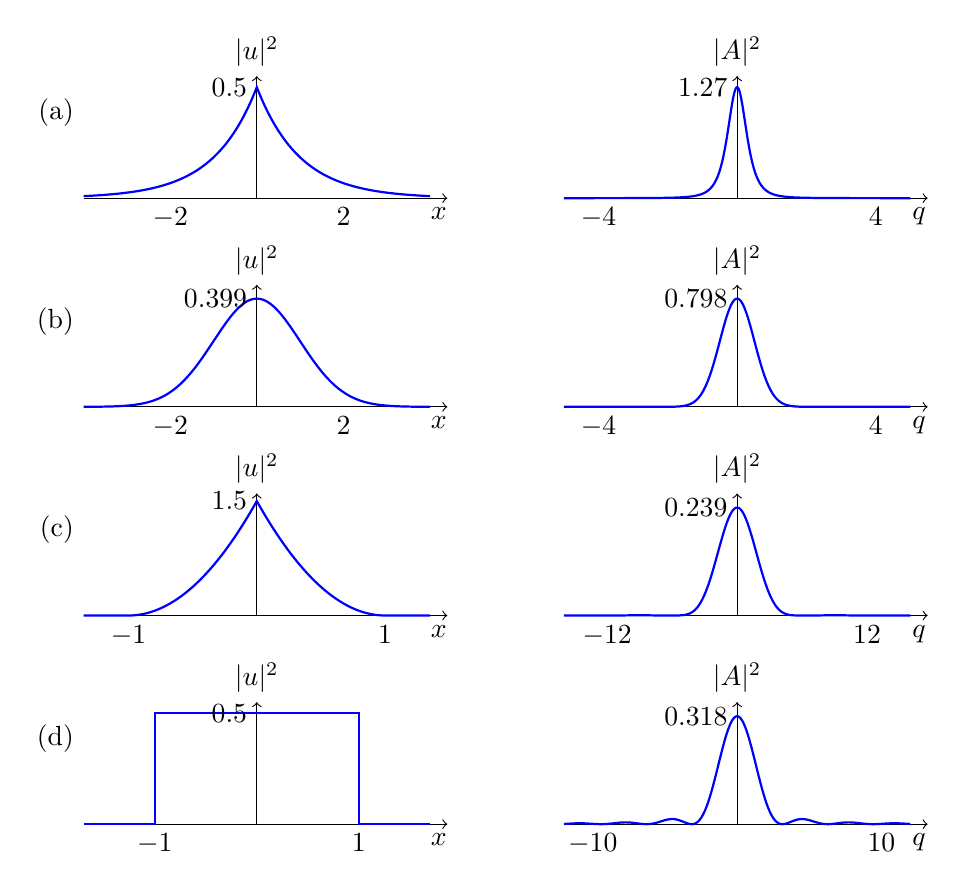
\begin{tikzpicture}
\begin{scope}[xshift=0.0cm,yshift=0.0cm,x=0.55cm,y=2.818181818181818cm]
\draw[->] (-4.0,0)--(4.4,0);\draw[->] (0,0)--(0,0.55) node[above] {$|u|^2$};
\draw[blue,thick] plot coordinates {(-4.000000,0.009158) (-3.986667,0.009281) (-3.973333,0.009405) (-3.960000,0.009532) (-3.946667,0.009659) (-3.933333,0.009789) (-3.920000,0.009921) (-3.906667,0.010054) (-3.893333,0.010189) (-3.880000,0.010325) (-3.866667,0.010464) (-3.853333,0.010604) (-3.840000,0.010747) (-3.826667,0.010891) (-3.813333,0.011037) (-3.800000,0.011185) (-3.786667,0.011336) (-3.773333,0.011488) (-3.760000,0.011642) (-3.746667,0.011798) (-3.733333,0.011956) (-3.720000,0.012117) (-3.706667,0.012280) (-3.693333,0.012444) (-3.680000,0.012611) (-3.666667,0.012781) (-3.653333,0.012952) (-3.640000,0.013126) (-3.626667,0.013302) (-3.613333,0.013481) (-3.600000,0.013662) (-3.586667,0.013845) (-3.573333,0.014031) (-3.560000,0.014219) (-3.546667,0.014410) (-3.533333,0.014604) (-3.520000,0.014800) (-3.506667,0.014998) (-3.493333,0.015200) (-3.480000,0.015404) (-3.466667,0.015610) (-3.453333,0.015820) (-3.440000,0.016032) (-3.426667,0.016248) (-3.413333,0.016466) (-3.400000,0.016687) (-3.386667,0.016911) (-3.373333,0.017138) (-3.360000,0.017368) (-3.346667,0.017601) (-3.333333,0.017837) (-3.320000,0.018076) (-3.306667,0.018319) (-3.293333,0.018565) (-3.280000,0.018814) (-3.266667,0.019067) (-3.253333,0.019323) (-3.240000,0.019582) (-3.226667,0.019845) (-3.213333,0.020111) (-3.200000,0.020381) (-3.186667,0.020655) (-3.173333,0.020932) (-3.160000,0.021213) (-3.146667,0.021498) (-3.133333,0.021786) (-3.120000,0.022079) (-3.106667,0.022375) (-3.093333,0.022675) (-3.080000,0.022980) (-3.066667,0.023288) (-3.053333,0.023601) (-3.040000,0.023917) (-3.026667,0.024238) (-3.013333,0.024564) (-3.000000,0.024894) (-2.986667,0.025228) (-2.973333,0.025566) (-2.960000,0.025909) (-2.946667,0.026257) (-2.933333,0.026610) (-2.920000,0.026967) (-2.906667,0.027329) (-2.893333,0.027696) (-2.880000,0.028067) (-2.866667,0.028444) (-2.853333,0.028826) (-2.840000,0.029213) (-2.826667,0.029605) (-2.813333,0.030002) (-2.800000,0.030405) (-2.786667,0.030813) (-2.773333,0.031227) (-2.760000,0.031646) (-2.746667,0.032071) (-2.733333,0.032501) (-2.720000,0.032937) (-2.706667,0.033379) (-2.693333,0.033828) (-2.680000,0.034282) (-2.666667,0.034742) (-2.653333,0.035208) (-2.640000,0.035681) (-2.626667,0.036160) (-2.613333,0.036645) (-2.600000,0.037137) (-2.586667,0.037635) (-2.573333,0.038140) (-2.560000,0.038652) (-2.546667,0.039171) (-2.533333,0.039697) (-2.520000,0.040230) (-2.506667,0.040770) (-2.493333,0.041317) (-2.480000,0.041872) (-2.466667,0.042434) (-2.453333,0.043003) (-2.440000,0.043580) (-2.426667,0.044165) (-2.413333,0.044758) (-2.400000,0.045359) (-2.386667,0.045968) (-2.373333,0.046585) (-2.360000,0.047210) (-2.346667,0.047844) (-2.333333,0.048486) (-2.320000,0.049137) (-2.306667,0.049796) (-2.293333,0.050465) (-2.280000,0.051142) (-2.266667,0.051829) (-2.253333,0.052524) (-2.240000,0.053229) (-2.226667,0.053944) (-2.213333,0.054668) (-2.200000,0.055402) (-2.186667,0.056145) (-2.173333,0.056899) (-2.160000,0.057663) (-2.146667,0.058437) (-2.133333,0.059221) (-2.120000,0.060016) (-2.106667,0.060821) (-2.093333,0.061638) (-2.080000,0.062465) (-2.066667,0.063304) (-2.053333,0.064153) (-2.040000,0.065014) (-2.026667,0.065887) (-2.013333,0.066771) (-2.000000,0.067668) (-1.986667,0.068576) (-1.973333,0.069496) (-1.960000,0.070429) (-1.946667,0.071375) (-1.933333,0.072333) (-1.920000,0.073303) (-1.906667,0.074287) (-1.893333,0.075285) (-1.880000,0.076295) (-1.866667,0.077319) (-1.853333,0.078357) (-1.840000,0.079409) (-1.826667,0.080475) (-1.813333,0.081555) (-1.800000,0.082649) (-1.786667,0.083759) (-1.773333,0.084883) (-1.760000,0.086022) (-1.746667,0.087177) (-1.733333,0.088347) (-1.720000,0.089533) (-1.706667,0.090735) (-1.693333,0.091953) (-1.680000,0.093187) (-1.666667,0.094438) (-1.653333,0.095705) (-1.640000,0.096990) (-1.626667,0.098292) (-1.613333,0.099611) (-1.600000,0.100948) (-1.586667,0.102303) (-1.573333,0.103676) (-1.560000,0.105068) (-1.546667,0.106478) (-1.533333,0.107908) (-1.520000,0.109356) (-1.506667,0.110824) (-1.493333,0.112311) (-1.480000,0.113819) (-1.466667,0.115347) (-1.453333,0.116895) (-1.440000,0.118464) (-1.426667,0.120054) (-1.413333,0.121665) (-1.400000,0.123298) (-1.386667,0.124953) (-1.373333,0.126631) (-1.360000,0.128330) (-1.346667,0.130053) (-1.333333,0.131799) (-1.320000,0.133568) (-1.306667,0.135360) (-1.293333,0.137177) (-1.280000,0.139019) (-1.266667,0.140885) (-1.253333,0.142776) (-1.240000,0.144692) (-1.226667,0.146634) (-1.213333,0.148602) (-1.200000,0.150597) (-1.186667,0.152619) (-1.173333,0.154667) (-1.160000,0.156743) (-1.146667,0.158847) (-1.133333,0.160979) (-1.120000,0.163140) (-1.106667,0.165330) (-1.093333,0.167549) (-1.080000,0.169798) (-1.066667,0.172077) (-1.053333,0.174387) (-1.040000,0.176727) (-1.026667,0.179099) (-1.013333,0.181503) (-1.000000,0.183940) (-0.986667,0.186409) (-0.973333,0.188911) (-0.960000,0.191446) (-0.946667,0.194016) (-0.933333,0.196620) (-0.920000,0.199260) (-0.906667,0.201934) (-0.893333,0.204645) (-0.880000,0.207391) (-0.866667,0.210175) (-0.853333,0.212996) (-0.840000,0.215855) (-0.826667,0.218753) (-0.813333,0.221689) (-0.800000,0.224664) (-0.786667,0.227680) (-0.773333,0.230736) (-0.760000,0.233833) (-0.746667,0.236972) (-0.733333,0.240153) (-0.720000,0.243376) (-0.706667,0.246643) (-0.693333,0.249953) (-0.680000,0.253308) (-0.666667,0.256709) (-0.653333,0.260154) (-0.640000,0.263646) (-0.626667,0.267185) (-0.613333,0.270771) (-0.600000,0.274406) (-0.586667,0.278089) (-0.573333,0.281822) (-0.560000,0.285605) (-0.546667,0.289438) (-0.533333,0.293323) (-0.520000,0.297260) (-0.506667,0.301250) (-0.493333,0.305294) (-0.480000,0.309392) (-0.466667,0.313545) (-0.453333,0.317753) (-0.440000,0.322018) (-0.426667,0.326341) (-0.413333,0.330721) (-0.400000,0.335160) (-0.386667,0.339659) (-0.373333,0.344218) (-0.360000,0.348838) (-0.346667,0.353520) (-0.333333,0.358266) (-0.320000,0.363075) (-0.306667,0.367948) (-0.293333,0.372887) (-0.280000,0.377892) (-0.266667,0.382964) (-0.253333,0.388105) (-0.240000,0.393314) (-0.226667,0.398593) (-0.213333,0.403943) (-0.200000,0.409365) (-0.186667,0.414860) (-0.173333,0.420429) (-0.160000,0.426072) (-0.146667,0.431791) (-0.133333,0.437587) (-0.120000,0.443460) (-0.106667,0.449413) (-0.093333,0.455445) (-0.080000,0.461558) (-0.066667,0.467753) (-0.053333,0.474032) (-0.040000,0.480395) (-0.026667,0.486843) (-0.013333,0.493378) (0.000000,0.500000) (0.013333,0.493378) (0.026667,0.486843) (0.040000,0.480395) (0.053333,0.474032) (0.066667,0.467753) (0.080000,0.461558) (0.093333,0.455445) (0.106667,0.449413) (0.120000,0.443460) (0.133333,0.437587) (0.146667,0.431791) (0.160000,0.426072) (0.173333,0.420429) (0.186667,0.414860) (0.200000,0.409365) (0.213333,0.403943) (0.226667,0.398593) (0.240000,0.393314) (0.253333,0.388105) (0.266667,0.382964) (0.280000,0.377892) (0.293333,0.372887) (0.306667,0.367948) (0.320000,0.363075) (0.333333,0.358266) (0.346667,0.353520) (0.360000,0.348838) (0.373333,0.344218) (0.386667,0.339659) (0.400000,0.335160) (0.413333,0.330721) (0.426667,0.326341) (0.440000,0.322018) (0.453333,0.317753) (0.466667,0.313545) (0.480000,0.309392) (0.493333,0.305294) (0.506667,0.301250) (0.520000,0.297260) (0.533333,0.293323) (0.546667,0.289438) (0.560000,0.285605) (0.573333,0.281822) (0.586667,0.278089) (0.600000,0.274406) (0.613333,0.270771) (0.626667,0.267185) (0.640000,0.263646) (0.653333,0.260154) (0.666667,0.256709) (0.680000,0.253308) (0.693333,0.249953) (0.706667,0.246643) (0.720000,0.243376) (0.733333,0.240153) (0.746667,0.236972) (0.760000,0.233833) (0.773333,0.230736) (0.786667,0.227680) (0.800000,0.224664) (0.813333,0.221689) (0.826667,0.218753) (0.840000,0.215855) (0.853333,0.212996) (0.866667,0.210175) (0.880000,0.207391) (0.893333,0.204645) (0.906667,0.201934) (0.920000,0.199260) (0.933333,0.196620) (0.946667,0.194016) (0.960000,0.191446) (0.973333,0.188911) (0.986667,0.186409) (1.000000,0.183940) (1.013333,0.181503) (1.026667,0.179099) (1.040000,0.176727) (1.053333,0.174387) (1.066667,0.172077) (1.080000,0.169798) (1.093333,0.167549) (1.106667,0.165330) (1.120000,0.163140) (1.133333,0.160979) (1.146667,0.158847) (1.160000,0.156743) (1.173333,0.154667) (1.186667,0.152619) (1.200000,0.150597) (1.213333,0.148602) (1.226667,0.146634) (1.240000,0.144692) (1.253333,0.142776) (1.266667,0.140885) (1.280000,0.139019) (1.293333,0.137177) (1.306667,0.135360) (1.320000,0.133568) (1.333333,0.131799) (1.346667,0.130053) (1.360000,0.128330) (1.373333,0.126631) (1.386667,0.124953) (1.400000,0.123298) (1.413333,0.121665) (1.426667,0.120054) (1.440000,0.118464) (1.453333,0.116895) (1.466667,0.115347) (1.480000,0.113819) (1.493333,0.112311) (1.506667,0.110824) (1.520000,0.109356) (1.533333,0.107908) (1.546667,0.106478) (1.560000,0.105068) (1.573333,0.103676) (1.586667,0.102303) (1.600000,0.100948) (1.613333,0.099611) (1.626667,0.098292) (1.640000,0.096990) (1.653333,0.095705) (1.666667,0.094438) (1.680000,0.093187) (1.693333,0.091953) (1.706667,0.090735) (1.720000,0.089533) (1.733333,0.088347) (1.746667,0.087177) (1.760000,0.086022) (1.773333,0.084883) (1.786667,0.083759) (1.800000,0.082649) (1.813333,0.081555) (1.826667,0.080475) (1.840000,0.079409) (1.853333,0.078357) (1.866667,0.077319) (1.880000,0.076295) (1.893333,0.075285) (1.906667,0.074287) (1.920000,0.073303) (1.933333,0.072333) (1.946667,0.071375) (1.960000,0.070429) (1.973333,0.069496) (1.986667,0.068576) (2.000000,0.067668) (2.013333,0.066771) (2.026667,0.065887) (2.040000,0.065014) (2.053333,0.064153) (2.066667,0.063304) (2.080000,0.062465) (2.093333,0.061638) (2.106667,0.060821) (2.120000,0.060016) (2.133333,0.059221) (2.146667,0.058437) (2.160000,0.057663) (2.173333,0.056899) (2.186667,0.056145) (2.200000,0.055402) (2.213333,0.054668) (2.226667,0.053944) (2.240000,0.053229) (2.253333,0.052524) (2.266667,0.051829) (2.280000,0.051142) (2.293333,0.050465) (2.306667,0.049796) (2.320000,0.049137) (2.333333,0.048486) (2.346667,0.047844) (2.360000,0.047210) (2.373333,0.046585) (2.386667,0.045968) (2.400000,0.045359) (2.413333,0.044758) (2.426667,0.044165) (2.440000,0.043580) (2.453333,0.043003) (2.466667,0.042434) (2.480000,0.041872) (2.493333,0.041317) (2.506667,0.040770) (2.520000,0.040230) (2.533333,0.039697) (2.546667,0.039171) (2.560000,0.038652) (2.573333,0.038140) (2.586667,0.037635) (2.600000,0.037137) (2.613333,0.036645) (2.626667,0.036160) (2.640000,0.035681) (2.653333,0.035208) (2.666667,0.034742) (2.680000,0.034282) (2.693333,0.033828) (2.706667,0.033379) (2.720000,0.032937) (2.733333,0.032501) (2.746667,0.032071) (2.760000,0.031646) (2.773333,0.031227) (2.786667,0.030813) (2.800000,0.030405) (2.813333,0.030002) (2.826667,0.029605) (2.840000,0.029213) (2.853333,0.028826) (2.866667,0.028444) (2.880000,0.028067) (2.893333,0.027696) (2.906667,0.027329) (2.920000,0.026967) (2.933333,0.026610) (2.946667,0.026257) (2.960000,0.025909) (2.973333,0.025566) (2.986667,0.025228) (3.000000,0.024894) (3.013333,0.024564) (3.026667,0.024238) (3.040000,0.023917) (3.053333,0.023601) (3.066667,0.023288) (3.080000,0.022980) (3.093333,0.022675) (3.106667,0.022375) (3.120000,0.022079) (3.133333,0.021786) (3.146667,0.021498) (3.160000,0.021213) (3.173333,0.020932) (3.186667,0.020655) (3.200000,0.020381) (3.213333,0.020111) (3.226667,0.019845) (3.240000,0.019582) (3.253333,0.019323) (3.266667,0.019067) (3.280000,0.018814) (3.293333,0.018565) (3.306667,0.018319) (3.320000,0.018076) (3.333333,0.017837) (3.346667,0.017601) (3.360000,0.017368) (3.373333,0.017138) (3.386667,0.016911) (3.400000,0.016687) (3.413333,0.016466) (3.426667,0.016248) (3.440000,0.016032) (3.453333,0.015820) (3.466667,0.015610) (3.480000,0.015404) (3.493333,0.015200) (3.506667,0.014998) (3.520000,0.014800) (3.533333,0.014604) (3.546667,0.014410) (3.560000,0.014219) (3.573333,0.014031) (3.586667,0.013845) (3.600000,0.013662) (3.613333,0.013481) (3.626667,0.013302) (3.640000,0.013126) (3.653333,0.012952) (3.666667,0.012781) (3.680000,0.012611) (3.693333,0.012444) (3.706667,0.012280) (3.720000,0.012117) (3.733333,0.011956) (3.746667,0.011798) (3.760000,0.011642) (3.773333,0.011488) (3.786667,0.011336) (3.800000,0.011185) (3.813333,0.011037) (3.826667,0.010891) (3.840000,0.010747) (3.853333,0.010604) (3.866667,0.010464) (3.880000,0.010325) (3.893333,0.010189) (3.906667,0.010054) (3.920000,0.009921) (3.933333,0.009789) (3.946667,0.009659) (3.960000,0.009532) (3.973333,0.009405) (3.986667,0.009281) (4.000000,0.009158)};
\node[below] at (-2.0,0) {$-2$};
\node[below] at (2.0,0) {$2$};
\node[left] at (0,0.5) {$0.5$};
\node[below] at (4.2,0) {$x$};
\node[left] at (-4.0,0.385) {(a)};
\end{scope}
\begin{scope}[xshift=6.1cm,yshift=0.0cm,x=0.44000000000000006cm,y=1.1071428571428572cm]
\draw[->] (-5.0,0)--(5.5,0);\draw[->] (0,0)--(0,1.4) node[above] {$|A|^2$};
\draw[blue,thick] plot coordinates {(-5.000000,0.000125) (-4.983333,0.000126) (-4.966667,0.000128) (-4.950000,0.000130) (-4.933333,0.000132) (-4.916667,0.000133) (-4.900000,0.000135) (-4.883333,0.000137) (-4.866667,0.000139) (-4.850000,0.000141) (-4.833333,0.000143) (-4.816667,0.000145) (-4.800000,0.000147) (-4.783333,0.000149) (-4.766667,0.000151) (-4.750000,0.000153) (-4.733333,0.000155) (-4.716667,0.000157) (-4.700000,0.000159) (-4.683333,0.000162) (-4.666667,0.000164) (-4.650000,0.000166) (-4.633333,0.000169) (-4.616667,0.000171) (-4.600000,0.000174) (-4.583333,0.000176) (-4.566667,0.000179) (-4.550000,0.000181) (-4.533333,0.000184) (-4.516667,0.000187) (-4.500000,0.000189) (-4.483333,0.000192) (-4.466667,0.000195) (-4.450000,0.000198) (-4.433333,0.000201) (-4.416667,0.000204) (-4.400000,0.000207) (-4.383333,0.000210) (-4.366667,0.000213) (-4.350000,0.000216) (-4.333333,0.000220) (-4.316667,0.000223) (-4.300000,0.000227) (-4.283333,0.000230) (-4.266667,0.000234) (-4.250000,0.000237) (-4.233333,0.000241) (-4.216667,0.000245) (-4.200000,0.000249) (-4.183333,0.000253) (-4.166667,0.000257) (-4.150000,0.000261) (-4.133333,0.000265) (-4.116667,0.000269) (-4.100000,0.000273) (-4.083333,0.000278) (-4.066667,0.000282) (-4.050000,0.000287) (-4.033333,0.000292) (-4.016667,0.000296) (-4.000000,0.000301) (-3.983333,0.000306) (-3.966667,0.000311) (-3.950000,0.000317) (-3.933333,0.000322) (-3.916667,0.000327) (-3.900000,0.000333) (-3.883333,0.000339) (-3.866667,0.000344) (-3.850000,0.000350) (-3.833333,0.000356) (-3.816667,0.000362) (-3.800000,0.000369) (-3.783333,0.000375) (-3.766667,0.000382) (-3.750000,0.000388) (-3.733333,0.000395) (-3.716667,0.000402) (-3.700000,0.000410) (-3.683333,0.000417) (-3.666667,0.000424) (-3.650000,0.000432) (-3.633333,0.000440) (-3.616667,0.000448) (-3.600000,0.000456) (-3.583333,0.000464) (-3.566667,0.000473) (-3.550000,0.000482) (-3.533333,0.000491) (-3.516667,0.000500) (-3.500000,0.000509) (-3.483333,0.000519) (-3.466667,0.000529) (-3.450000,0.000539) (-3.433333,0.000549) (-3.416667,0.000560) (-3.400000,0.000571) (-3.383333,0.000582) (-3.366667,0.000593) (-3.350000,0.000605) (-3.333333,0.000617) (-3.316667,0.000629) (-3.300000,0.000641) (-3.283333,0.000654) (-3.266667,0.000667) (-3.250000,0.000681) (-3.233333,0.000694) (-3.216667,0.000709) (-3.200000,0.000723) (-3.183333,0.000738) (-3.166667,0.000753) (-3.150000,0.000769) (-3.133333,0.000785) (-3.116667,0.000802) (-3.100000,0.000819) (-3.083333,0.000836) (-3.066667,0.000854) (-3.050000,0.000872) (-3.033333,0.000891) (-3.016667,0.000910) (-3.000000,0.000930) (-2.983333,0.000950) (-2.966667,0.000971) (-2.950000,0.000993) (-2.933333,0.001015) (-2.916667,0.001038) (-2.900000,0.001061) (-2.883333,0.001085) (-2.866667,0.001110) (-2.850000,0.001135) (-2.833333,0.001161) (-2.816667,0.001188) (-2.800000,0.001216) (-2.783333,0.001244) (-2.766667,0.001274) (-2.750000,0.001304) (-2.733333,0.001335) (-2.716667,0.001367) (-2.700000,0.001400) (-2.683333,0.001434) (-2.666667,0.001469) (-2.650000,0.001505) (-2.633333,0.001542) (-2.616667,0.001580) (-2.600000,0.001619) (-2.583333,0.001660) (-2.566667,0.001702) (-2.550000,0.001745) (-2.533333,0.001790) (-2.516667,0.001836) (-2.500000,0.001883) (-2.483333,0.001933) (-2.466667,0.001983) (-2.450000,0.002036) (-2.433333,0.002090) (-2.416667,0.002145) (-2.400000,0.002203) (-2.383333,0.002263) (-2.366667,0.002324) (-2.350000,0.002388) (-2.333333,0.002454) (-2.316667,0.002522) (-2.300000,0.002593) (-2.283333,0.002666) (-2.266667,0.002741) (-2.250000,0.002820) (-2.233333,0.002901) (-2.216667,0.002985) (-2.200000,0.003072) (-2.183333,0.003162) (-2.166667,0.003255) (-2.150000,0.003352) (-2.133333,0.003452) (-2.116667,0.003556) (-2.100000,0.003665) (-2.083333,0.003777) (-2.066667,0.003893) (-2.050000,0.004014) (-2.033333,0.004140) (-2.016667,0.004270) (-2.000000,0.004406) (-1.983333,0.004547) (-1.966667,0.004693) (-1.950000,0.004846) (-1.933333,0.005004) (-1.916667,0.005169) (-1.900000,0.005341) (-1.883333,0.005520) (-1.866667,0.005706) (-1.850000,0.005900) (-1.833333,0.006103) (-1.816667,0.006313) (-1.800000,0.006533) (-1.783333,0.006763) (-1.766667,0.007002) (-1.750000,0.007252) (-1.733333,0.007513) (-1.716667,0.007786) (-1.700000,0.008071) (-1.683333,0.008369) (-1.666667,0.008680) (-1.650000,0.009006) (-1.633333,0.009347) (-1.616667,0.009704) (-1.600000,0.010078) (-1.583333,0.010470) (-1.566667,0.010880) (-1.550000,0.011310) (-1.533333,0.011762) (-1.516667,0.012235) (-1.500000,0.012732) (-1.483333,0.013254) (-1.466667,0.013803) (-1.450000,0.014379) (-1.433333,0.014985) (-1.416667,0.015622) (-1.400000,0.016293) (-1.383333,0.016999) (-1.366667,0.017743) (-1.350000,0.018527) (-1.333333,0.019353) (-1.316667,0.020224) (-1.300000,0.021144) (-1.283333,0.022115) (-1.266667,0.023140) (-1.250000,0.024223) (-1.233333,0.025369) (-1.216667,0.026580) (-1.200000,0.027862) (-1.183333,0.029220) (-1.166667,0.030658) (-1.150000,0.032182) (-1.133333,0.033798) (-1.116667,0.035512) (-1.100000,0.037332) (-1.083333,0.039265) (-1.066667,0.041319) (-1.050000,0.043503) (-1.033333,0.045825) (-1.016667,0.048297) (-1.000000,0.050930) (-0.983333,0.053734) (-0.966667,0.056723) (-0.950000,0.059911) (-0.933333,0.063313) (-0.916667,0.066945) (-0.900000,0.070824) (-0.883333,0.074969) (-0.866667,0.079401) (-0.850000,0.084142) (-0.833333,0.089215) (-0.816667,0.094646) (-0.800000,0.100464) (-0.783333,0.106697) (-0.766667,0.113379) (-0.750000,0.120543) (-0.733333,0.128228) (-0.716667,0.136473) (-0.700000,0.145320) (-0.683333,0.154817) (-0.666667,0.165012) (-0.650000,0.175957) (-0.633333,0.187707) (-0.616667,0.200321) (-0.600000,0.213860) (-0.583333,0.228390) (-0.566667,0.243977) (-0.550000,0.260691) (-0.533333,0.278602) (-0.516667,0.297785) (-0.500000,0.318310) (-0.483333,0.340250) (-0.466667,0.363673) (-0.450000,0.388645) (-0.433333,0.415224) (-0.416667,0.443461) (-0.400000,0.473394) (-0.383333,0.505046) (-0.366667,0.538422) (-0.350000,0.573505) (-0.333333,0.610251) (-0.316667,0.648582) (-0.300000,0.688386) (-0.283333,0.729510) (-0.266667,0.771755) (-0.250000,0.814873) (-0.233333,0.858567) (-0.216667,0.902484) (-0.200000,0.946224) (-0.183333,0.989336) (-0.166667,1.031324) (-0.150000,1.071660) (-0.133333,1.109791) (-0.116667,1.145151) (-0.100000,1.177182) (-0.083333,1.205346) (-0.066667,1.229148) (-0.050000,1.248152) (-0.033333,1.261997) (-0.016667,1.270415) (0.000000,1.273240) (0.016667,1.270415) (0.033333,1.261997) (0.050000,1.248152) (0.066667,1.229148) (0.083333,1.205346) (0.100000,1.177182) (0.116667,1.145151) (0.133333,1.109791) (0.150000,1.071660) (0.166667,1.031324) (0.183333,0.989336) (0.200000,0.946224) (0.216667,0.902484) (0.233333,0.858567) (0.250000,0.814873) (0.266667,0.771755) (0.283333,0.729510) (0.300000,0.688386) (0.316667,0.648582) (0.333333,0.610251) (0.350000,0.573505) (0.366667,0.538422) (0.383333,0.505046) (0.400000,0.473394) (0.416667,0.443461) (0.433333,0.415224) (0.450000,0.388645) (0.466667,0.363673) (0.483333,0.340250) (0.500000,0.318310) (0.516667,0.297785) (0.533333,0.278602) (0.550000,0.260691) (0.566667,0.243977) (0.583333,0.228390) (0.600000,0.213860) (0.616667,0.200321) (0.633333,0.187707) (0.650000,0.175957) (0.666667,0.165012) (0.683333,0.154817) (0.700000,0.145320) (0.716667,0.136473) (0.733333,0.128228) (0.750000,0.120543) (0.766667,0.113379) (0.783333,0.106697) (0.800000,0.100464) (0.816667,0.094646) (0.833333,0.089215) (0.850000,0.084142) (0.866667,0.079401) (0.883333,0.074969) (0.900000,0.070824) (0.916667,0.066945) (0.933333,0.063313) (0.950000,0.059911) (0.966667,0.056723) (0.983333,0.053734) (1.000000,0.050930) (1.016667,0.048297) (1.033333,0.045825) (1.050000,0.043503) (1.066667,0.041319) (1.083333,0.039265) (1.100000,0.037332) (1.116667,0.035512) (1.133333,0.033798) (1.150000,0.032182) (1.166667,0.030658) (1.183333,0.029220) (1.200000,0.027862) (1.216667,0.026580) (1.233333,0.025369) (1.250000,0.024223) (1.266667,0.023140) (1.283333,0.022115) (1.300000,0.021144) (1.316667,0.020224) (1.333333,0.019353) (1.350000,0.018527) (1.366667,0.017743) (1.383333,0.016999) (1.400000,0.016293) (1.416667,0.015622) (1.433333,0.014985) (1.450000,0.014379) (1.466667,0.013803) (1.483333,0.013254) (1.500000,0.012732) (1.516667,0.012235) (1.533333,0.011762) (1.550000,0.011310) (1.566667,0.010880) (1.583333,0.010470) (1.600000,0.010078) (1.616667,0.009704) (1.633333,0.009347) (1.650000,0.009006) (1.666667,0.008680) (1.683333,0.008369) (1.700000,0.008071) (1.716667,0.007786) (1.733333,0.007513) (1.750000,0.007252) (1.766667,0.007002) (1.783333,0.006763) (1.800000,0.006533) (1.816667,0.006313) (1.833333,0.006103) (1.850000,0.005900) (1.866667,0.005706) (1.883333,0.005520) (1.900000,0.005341) (1.916667,0.005169) (1.933333,0.005004) (1.950000,0.004846) (1.966667,0.004693) (1.983333,0.004547) (2.000000,0.004406) (2.016667,0.004270) (2.033333,0.004140) (2.050000,0.004014) (2.066667,0.003893) (2.083333,0.003777) (2.100000,0.003665) (2.116667,0.003556) (2.133333,0.003452) (2.150000,0.003352) (2.166667,0.003255) (2.183333,0.003162) (2.200000,0.003072) (2.216667,0.002985) (2.233333,0.002901) (2.250000,0.002820) (2.266667,0.002741) (2.283333,0.002666) (2.300000,0.002593) (2.316667,0.002522) (2.333333,0.002454) (2.350000,0.002388) (2.366667,0.002324) (2.383333,0.002263) (2.400000,0.002203) (2.416667,0.002145) (2.433333,0.002090) (2.450000,0.002036) (2.466667,0.001983) (2.483333,0.001933) (2.500000,0.001883) (2.516667,0.001836) (2.533333,0.001790) (2.550000,0.001745) (2.566667,0.001702) (2.583333,0.001660) (2.600000,0.001619) (2.616667,0.001580) (2.633333,0.001542) (2.650000,0.001505) (2.666667,0.001469) (2.683333,0.001434) (2.700000,0.001400) (2.716667,0.001367) (2.733333,0.001335) (2.750000,0.001304) (2.766667,0.001274) (2.783333,0.001244) (2.800000,0.001216) (2.816667,0.001188) (2.833333,0.001161) (2.850000,0.001135) (2.866667,0.001110) (2.883333,0.001085) (2.900000,0.001061) (2.916667,0.001038) (2.933333,0.001015) (2.950000,0.000993) (2.966667,0.000971) (2.983333,0.000950) (3.000000,0.000930) (3.016667,0.000910) (3.033333,0.000891) (3.050000,0.000872) (3.066667,0.000854) (3.083333,0.000836) (3.100000,0.000819) (3.116667,0.000802) (3.133333,0.000785) (3.150000,0.000769) (3.166667,0.000753) (3.183333,0.000738) (3.200000,0.000723) (3.216667,0.000709) (3.233333,0.000694) (3.250000,0.000681) (3.266667,0.000667) (3.283333,0.000654) (3.300000,0.000641) (3.316667,0.000629) (3.333333,0.000617) (3.350000,0.000605) (3.366667,0.000593) (3.383333,0.000582) (3.400000,0.000571) (3.416667,0.000560) (3.433333,0.000549) (3.450000,0.000539) (3.466667,0.000529) (3.483333,0.000519) (3.500000,0.000509) (3.516667,0.000500) (3.533333,0.000491) (3.550000,0.000482) (3.566667,0.000473) (3.583333,0.000464) (3.600000,0.000456) (3.616667,0.000448) (3.633333,0.000440) (3.650000,0.000432) (3.666667,0.000424) (3.683333,0.000417) (3.700000,0.000410) (3.716667,0.000402) (3.733333,0.000395) (3.750000,0.000388) (3.766667,0.000382) (3.783333,0.000375) (3.800000,0.000369) (3.816667,0.000362) (3.833333,0.000356) (3.850000,0.000350) (3.866667,0.000344) (3.883333,0.000339) (3.900000,0.000333) (3.916667,0.000327) (3.933333,0.000322) (3.950000,0.000317) (3.966667,0.000311) (3.983333,0.000306) (4.000000,0.000301) (4.016667,0.000296) (4.033333,0.000292) (4.050000,0.000287) (4.066667,0.000282) (4.083333,0.000278) (4.100000,0.000273) (4.116667,0.000269) (4.133333,0.000265) (4.150000,0.000261) (4.166667,0.000257) (4.183333,0.000253) (4.200000,0.000249) (4.216667,0.000245) (4.233333,0.000241) (4.250000,0.000237) (4.266667,0.000234) (4.283333,0.000230) (4.300000,0.000227) (4.316667,0.000223) (4.333333,0.000220) (4.350000,0.000216) (4.366667,0.000213) (4.383333,0.000210) (4.400000,0.000207) (4.416667,0.000204) (4.433333,0.000201) (4.450000,0.000198) (4.466667,0.000195) (4.483333,0.000192) (4.500000,0.000189) (4.516667,0.000187) (4.533333,0.000184) (4.550000,0.000181) (4.566667,0.000179) (4.583333,0.000176) (4.600000,0.000174) (4.616667,0.000171) (4.633333,0.000169) (4.650000,0.000166) (4.666667,0.000164) (4.683333,0.000162) (4.700000,0.000159) (4.716667,0.000157) (4.733333,0.000155) (4.750000,0.000153) (4.766667,0.000151) (4.783333,0.000149) (4.800000,0.000147) (4.816667,0.000145) (4.833333,0.000143) (4.850000,0.000141) (4.866667,0.000139) (4.883333,0.000137) (4.900000,0.000135) (4.916667,0.000133) (4.933333,0.000132) (4.950000,0.000130) (4.966667,0.000128) (4.983333,0.000126) (5.000000,0.000125)};
\node[below] at (-4.0,0) {$-4$};
\node[below] at (4.0,0) {$4$};
\node[left] at (0,1.2732395447351628) {$1.27$};
\node[below] at (5.25,0) {$q$};
\end{scope}
\begin{scope}[xshift=0.0cm,yshift=-2.65cm,x=0.55cm,y=3.4444444444444446cm]
\draw[->] (-4.0,0)--(4.4,0);\draw[->] (0,0)--(0,0.45) node[above] {$|u|^2$};
\draw[blue,thick] plot coordinates {(-4.000000,0.000134) (-3.986667,0.000141) (-3.973333,0.000149) (-3.960000,0.000157) (-3.946667,0.000165) (-3.933333,0.000174) (-3.920000,0.000184) (-3.906667,0.000194) (-3.893333,0.000204) (-3.880000,0.000215) (-3.866667,0.000226) (-3.853333,0.000238) (-3.840000,0.000251) (-3.826667,0.000264) (-3.813333,0.000277) (-3.800000,0.000292) (-3.786667,0.000307) (-3.773333,0.000323) (-3.760000,0.000340) (-3.746667,0.000357) (-3.733333,0.000375) (-3.720000,0.000394) (-3.706667,0.000414) (-3.693333,0.000435) (-3.680000,0.000457) (-3.666667,0.000480) (-3.653333,0.000504) (-3.640000,0.000529) (-3.626667,0.000556) (-3.613333,0.000583) (-3.600000,0.000612) (-3.586667,0.000642) (-3.573333,0.000673) (-3.560000,0.000706) (-3.546667,0.000740) (-3.533333,0.000776) (-3.520000,0.000814) (-3.506667,0.000853) (-3.493333,0.000893) (-3.480000,0.000936) (-3.466667,0.000980) (-3.453333,0.001026) (-3.440000,0.001075) (-3.426667,0.001125) (-3.413333,0.001178) (-3.400000,0.001232) (-3.386667,0.001289) (-3.373333,0.001349) (-3.360000,0.001411) (-3.346667,0.001475) (-3.333333,0.001542) (-3.320000,0.001612) (-3.306667,0.001685) (-3.293333,0.001761) (-3.280000,0.001840) (-3.266667,0.001922) (-3.253333,0.002007) (-3.240000,0.002096) (-3.226667,0.002188) (-3.213333,0.002284) (-3.200000,0.002384) (-3.186667,0.002488) (-3.173333,0.002596) (-3.160000,0.002707) (-3.146667,0.002824) (-3.133333,0.002944) (-3.120000,0.003070) (-3.106667,0.003200) (-3.093333,0.003335) (-3.080000,0.003475) (-3.066667,0.003620) (-3.053333,0.003771) (-3.040000,0.003928) (-3.026667,0.004090) (-3.013333,0.004258) (-3.000000,0.004432) (-2.986667,0.004612) (-2.973333,0.004799) (-2.960000,0.004993) (-2.946667,0.005193) (-2.933333,0.005401) (-2.920000,0.005616) (-2.906667,0.005838) (-2.893333,0.006069) (-2.880000,0.006307) (-2.866667,0.006553) (-2.853333,0.006808) (-2.840000,0.007071) (-2.826667,0.007343) (-2.813333,0.007625) (-2.800000,0.007915) (-2.786667,0.008216) (-2.773333,0.008526) (-2.760000,0.008846) (-2.746667,0.009177) (-2.733333,0.009519) (-2.720000,0.009871) (-2.706667,0.010235) (-2.693333,0.010610) (-2.680000,0.010997) (-2.666667,0.011396) (-2.653333,0.011807) (-2.640000,0.012232) (-2.626667,0.012669) (-2.613333,0.013119) (-2.600000,0.013583) (-2.586667,0.014061) (-2.573333,0.014553) (-2.560000,0.015060) (-2.546667,0.015581) (-2.533333,0.016118) (-2.520000,0.016670) (-2.506667,0.017238) (-2.493333,0.017822) (-2.480000,0.018423) (-2.466667,0.019041) (-2.453333,0.019676) (-2.440000,0.020328) (-2.426667,0.020999) (-2.413333,0.021687) (-2.400000,0.022395) (-2.386667,0.023121) (-2.373333,0.023866) (-2.360000,0.024631) (-2.346667,0.025416) (-2.333333,0.026222) (-2.320000,0.027048) (-2.306667,0.027895) (-2.293333,0.028764) (-2.280000,0.029655) (-2.266667,0.030567) (-2.253333,0.031502) (-2.240000,0.032460) (-2.226667,0.033441) (-2.213333,0.034446) (-2.200000,0.035475) (-2.186667,0.036527) (-2.173333,0.037605) (-2.160000,0.038707) (-2.146667,0.039834) (-2.133333,0.040987) (-2.120000,0.042166) (-2.106667,0.043371) (-2.093333,0.044603) (-2.080000,0.045861) (-2.066667,0.047147) (-2.053333,0.048459) (-2.040000,0.049800) (-2.026667,0.051169) (-2.013333,0.052566) (-2.000000,0.053991) (-1.986667,0.055445) (-1.973333,0.056928) (-1.960000,0.058441) (-1.946667,0.059983) (-1.933333,0.061555) (-1.920000,0.063157) (-1.906667,0.064788) (-1.893333,0.066451) (-1.880000,0.068144) (-1.866667,0.069867) (-1.853333,0.071621) (-1.840000,0.073407) (-1.826667,0.075223) (-1.813333,0.077071) (-1.800000,0.078950) (-1.786667,0.080861) (-1.773333,0.082803) (-1.760000,0.084776) (-1.746667,0.086782) (-1.733333,0.088818) (-1.720000,0.090887) (-1.706667,0.092987) (-1.693333,0.095119) (-1.680000,0.097282) (-1.666667,0.099477) (-1.653333,0.101703) (-1.640000,0.103961) (-1.626667,0.106250) (-1.613333,0.108570) (-1.600000,0.110921) (-1.586667,0.113302) (-1.573333,0.115715) (-1.560000,0.118157) (-1.546667,0.120630) (-1.533333,0.123133) (-1.520000,0.125665) (-1.506667,0.128226) (-1.493333,0.130816) (-1.480000,0.133435) (-1.466667,0.136082) (-1.453333,0.138758) (-1.440000,0.141460) (-1.426667,0.144189) (-1.413333,0.146945) (-1.400000,0.149727) (-1.386667,0.152535) (-1.373333,0.155368) (-1.360000,0.158225) (-1.346667,0.161106) (-1.333333,0.164010) (-1.320000,0.166937) (-1.306667,0.169886) (-1.293333,0.172856) (-1.280000,0.175847) (-1.266667,0.178858) (-1.253333,0.181889) (-1.240000,0.184937) (-1.226667,0.188004) (-1.213333,0.191087) (-1.200000,0.194186) (-1.186667,0.197300) (-1.173333,0.200429) (-1.160000,0.203571) (-1.146667,0.206726) (-1.133333,0.209892) (-1.120000,0.213069) (-1.106667,0.216256) (-1.093333,0.219451) (-1.080000,0.222653) (-1.066667,0.225863) (-1.053333,0.229078) (-1.040000,0.232297) (-1.026667,0.235520) (-1.013333,0.238745) (-1.000000,0.241971) (-0.986667,0.245197) (-0.973333,0.248422) (-0.960000,0.251644) (-0.946667,0.254863) (-0.933333,0.258078) (-0.920000,0.261286) (-0.906667,0.264488) (-0.893333,0.267681) (-0.880000,0.270864) (-0.866667,0.274036) (-0.853333,0.277197) (-0.840000,0.280344) (-0.826667,0.283476) (-0.813333,0.286592) (-0.800000,0.289692) (-0.786667,0.292772) (-0.773333,0.295833) (-0.760000,0.298872) (-0.746667,0.301890) (-0.733333,0.304883) (-0.720000,0.307851) (-0.706667,0.310793) (-0.693333,0.313708) (-0.680000,0.316593) (-0.666667,0.319448) (-0.653333,0.322272) (-0.640000,0.325062) (-0.626667,0.327819) (-0.613333,0.330540) (-0.600000,0.333225) (-0.586667,0.335871) (-0.573333,0.338479) (-0.560000,0.341046) (-0.546667,0.343571) (-0.533333,0.346054) (-0.520000,0.348493) (-0.506667,0.350886) (-0.493333,0.353233) (-0.480000,0.355533) (-0.466667,0.357783) (-0.453333,0.359985) (-0.440000,0.362135) (-0.426667,0.364233) (-0.413333,0.366279) (-0.400000,0.368270) (-0.386667,0.370207) (-0.373333,0.372087) (-0.360000,0.373911) (-0.346667,0.375676) (-0.333333,0.377383) (-0.320000,0.379031) (-0.306667,0.380617) (-0.293333,0.382143) (-0.280000,0.383606) (-0.266667,0.385007) (-0.253333,0.386344) (-0.240000,0.387617) (-0.226667,0.388824) (-0.213333,0.389967) (-0.200000,0.391043) (-0.186667,0.392052) (-0.173333,0.392994) (-0.160000,0.393868) (-0.146667,0.394674) (-0.133333,0.395412) (-0.120000,0.396080) (-0.106667,0.396679) (-0.093333,0.397208) (-0.080000,0.397668) (-0.066667,0.398057) (-0.053333,0.398375) (-0.040000,0.398623) (-0.026667,0.398800) (-0.013333,0.398907) (0.000000,0.398942) (0.013333,0.398907) (0.026667,0.398800) (0.040000,0.398623) (0.053333,0.398375) (0.066667,0.398057) (0.080000,0.397668) (0.093333,0.397208) (0.106667,0.396679) (0.120000,0.396080) (0.133333,0.395412) (0.146667,0.394674) (0.160000,0.393868) (0.173333,0.392994) (0.186667,0.392052) (0.200000,0.391043) (0.213333,0.389967) (0.226667,0.388824) (0.240000,0.387617) (0.253333,0.386344) (0.266667,0.385007) (0.280000,0.383606) (0.293333,0.382143) (0.306667,0.380617) (0.320000,0.379031) (0.333333,0.377383) (0.346667,0.375676) (0.360000,0.373911) (0.373333,0.372087) (0.386667,0.370207) (0.400000,0.368270) (0.413333,0.366279) (0.426667,0.364233) (0.440000,0.362135) (0.453333,0.359985) (0.466667,0.357783) (0.480000,0.355533) (0.493333,0.353233) (0.506667,0.350886) (0.520000,0.348493) (0.533333,0.346054) (0.546667,0.343571) (0.560000,0.341046) (0.573333,0.338479) (0.586667,0.335871) (0.600000,0.333225) (0.613333,0.330540) (0.626667,0.327819) (0.640000,0.325062) (0.653333,0.322272) (0.666667,0.319448) (0.680000,0.316593) (0.693333,0.313708) (0.706667,0.310793) (0.720000,0.307851) (0.733333,0.304883) (0.746667,0.301890) (0.760000,0.298872) (0.773333,0.295833) (0.786667,0.292772) (0.800000,0.289692) (0.813333,0.286592) (0.826667,0.283476) (0.840000,0.280344) (0.853333,0.277197) (0.866667,0.274036) (0.880000,0.270864) (0.893333,0.267681) (0.906667,0.264488) (0.920000,0.261286) (0.933333,0.258078) (0.946667,0.254863) (0.960000,0.251644) (0.973333,0.248422) (0.986667,0.245197) (1.000000,0.241971) (1.013333,0.238745) (1.026667,0.235520) (1.040000,0.232297) (1.053333,0.229078) (1.066667,0.225863) (1.080000,0.222653) (1.093333,0.219451) (1.106667,0.216256) (1.120000,0.213069) (1.133333,0.209892) (1.146667,0.206726) (1.160000,0.203571) (1.173333,0.200429) (1.186667,0.197300) (1.200000,0.194186) (1.213333,0.191087) (1.226667,0.188004) (1.240000,0.184937) (1.253333,0.181889) (1.266667,0.178858) (1.280000,0.175847) (1.293333,0.172856) (1.306667,0.169886) (1.320000,0.166937) (1.333333,0.164010) (1.346667,0.161106) (1.360000,0.158225) (1.373333,0.155368) (1.386667,0.152535) (1.400000,0.149727) (1.413333,0.146945) (1.426667,0.144189) (1.440000,0.141460) (1.453333,0.138758) (1.466667,0.136082) (1.480000,0.133435) (1.493333,0.130816) (1.506667,0.128226) (1.520000,0.125665) (1.533333,0.123133) (1.546667,0.120630) (1.560000,0.118157) (1.573333,0.115715) (1.586667,0.113302) (1.600000,0.110921) (1.613333,0.108570) (1.626667,0.106250) (1.640000,0.103961) (1.653333,0.101703) (1.666667,0.099477) (1.680000,0.097282) (1.693333,0.095119) (1.706667,0.092987) (1.720000,0.090887) (1.733333,0.088818) (1.746667,0.086782) (1.760000,0.084776) (1.773333,0.082803) (1.786667,0.080861) (1.800000,0.078950) (1.813333,0.077071) (1.826667,0.075223) (1.840000,0.073407) (1.853333,0.071621) (1.866667,0.069867) (1.880000,0.068144) (1.893333,0.066451) (1.906667,0.064788) (1.920000,0.063157) (1.933333,0.061555) (1.946667,0.059983) (1.960000,0.058441) (1.973333,0.056928) (1.986667,0.055445) (2.000000,0.053991) (2.013333,0.052566) (2.026667,0.051169) (2.040000,0.049800) (2.053333,0.048459) (2.066667,0.047147) (2.080000,0.045861) (2.093333,0.044603) (2.106667,0.043371) (2.120000,0.042166) (2.133333,0.040987) (2.146667,0.039834) (2.160000,0.038707) (2.173333,0.037605) (2.186667,0.036527) (2.200000,0.035475) (2.213333,0.034446) (2.226667,0.033441) (2.240000,0.032460) (2.253333,0.031502) (2.266667,0.030567) (2.280000,0.029655) (2.293333,0.028764) (2.306667,0.027895) (2.320000,0.027048) (2.333333,0.026222) (2.346667,0.025416) (2.360000,0.024631) (2.373333,0.023866) (2.386667,0.023121) (2.400000,0.022395) (2.413333,0.021687) (2.426667,0.020999) (2.440000,0.020328) (2.453333,0.019676) (2.466667,0.019041) (2.480000,0.018423) (2.493333,0.017822) (2.506667,0.017238) (2.520000,0.016670) (2.533333,0.016118) (2.546667,0.015581) (2.560000,0.015060) (2.573333,0.014553) (2.586667,0.014061) (2.600000,0.013583) (2.613333,0.013119) (2.626667,0.012669) (2.640000,0.012232) (2.653333,0.011807) (2.666667,0.011396) (2.680000,0.010997) (2.693333,0.010610) (2.706667,0.010235) (2.720000,0.009871) (2.733333,0.009519) (2.746667,0.009177) (2.760000,0.008846) (2.773333,0.008526) (2.786667,0.008216) (2.800000,0.007915) (2.813333,0.007625) (2.826667,0.007343) (2.840000,0.007071) (2.853333,0.006808) (2.866667,0.006553) (2.880000,0.006307) (2.893333,0.006069) (2.906667,0.005838) (2.920000,0.005616) (2.933333,0.005401) (2.946667,0.005193) (2.960000,0.004993) (2.973333,0.004799) (2.986667,0.004612) (3.000000,0.004432) (3.013333,0.004258) (3.026667,0.004090) (3.040000,0.003928) (3.053333,0.003771) (3.066667,0.003620) (3.080000,0.003475) (3.093333,0.003335) (3.106667,0.003200) (3.120000,0.003070) (3.133333,0.002944) (3.146667,0.002824) (3.160000,0.002707) (3.173333,0.002596) (3.186667,0.002488) (3.200000,0.002384) (3.213333,0.002284) (3.226667,0.002188) (3.240000,0.002096) (3.253333,0.002007) (3.266667,0.001922) (3.280000,0.001840) (3.293333,0.001761) (3.306667,0.001685) (3.320000,0.001612) (3.333333,0.001542) (3.346667,0.001475) (3.360000,0.001411) (3.373333,0.001349) (3.386667,0.001289) (3.400000,0.001232) (3.413333,0.001178) (3.426667,0.001125) (3.440000,0.001075) (3.453333,0.001026) (3.466667,0.000980) (3.480000,0.000936) (3.493333,0.000893) (3.506667,0.000853) (3.520000,0.000814) (3.533333,0.000776) (3.546667,0.000740) (3.560000,0.000706) (3.573333,0.000673) (3.586667,0.000642) (3.600000,0.000612) (3.613333,0.000583) (3.626667,0.000556) (3.640000,0.000529) (3.653333,0.000504) (3.666667,0.000480) (3.680000,0.000457) (3.693333,0.000435) (3.706667,0.000414) (3.720000,0.000394) (3.733333,0.000375) (3.746667,0.000357) (3.760000,0.000340) (3.773333,0.000323) (3.786667,0.000307) (3.800000,0.000292) (3.813333,0.000277) (3.826667,0.000264) (3.840000,0.000251) (3.853333,0.000238) (3.866667,0.000226) (3.880000,0.000215) (3.893333,0.000204) (3.906667,0.000194) (3.920000,0.000184) (3.933333,0.000174) (3.946667,0.000165) (3.960000,0.000157) (3.973333,0.000149) (3.986667,0.000141) (4.000000,0.000134)};
\node[below] at (-2.0,0) {$-2$};
\node[below] at (2.0,0) {$2$};
\node[left] at (0,0.3989422804014327) {$0.399$};
\node[below] at (4.2,0) {$x$};
\node[left] at (-4.0,0.315) {(b)};
\end{scope}
\begin{scope}[xshift=6.1cm,yshift=-2.65cm,x=0.44000000000000006cm,y=1.7222222222222223cm]
\draw[->] (-5.0,0)--(5.5,0);\draw[->] (0,0)--(0,0.9) node[above] {$|A|^2$};
\draw[blue,thick] plot coordinates {(-5.000000,0.000000) (-4.983333,0.000000) (-4.966667,0.000000) (-4.950000,0.000000) (-4.933333,0.000000) (-4.916667,0.000000) (-4.900000,0.000000) (-4.883333,0.000000) (-4.866667,0.000000) (-4.850000,0.000000) (-4.833333,0.000000) (-4.816667,0.000000) (-4.800000,0.000000) (-4.783333,0.000000) (-4.766667,0.000000) (-4.750000,0.000000) (-4.733333,0.000000) (-4.716667,0.000000) (-4.700000,0.000000) (-4.683333,0.000000) (-4.666667,0.000000) (-4.650000,0.000000) (-4.633333,0.000000) (-4.616667,0.000000) (-4.600000,0.000000) (-4.583333,0.000000) (-4.566667,0.000000) (-4.550000,0.000000) (-4.533333,0.000000) (-4.516667,0.000000) (-4.500000,0.000000) (-4.483333,0.000000) (-4.466667,0.000000) (-4.450000,0.000000) (-4.433333,0.000000) (-4.416667,0.000000) (-4.400000,0.000000) (-4.383333,0.000000) (-4.366667,0.000000) (-4.350000,0.000000) (-4.333333,0.000000) (-4.316667,0.000000) (-4.300000,0.000000) (-4.283333,0.000000) (-4.266667,0.000000) (-4.250000,0.000000) (-4.233333,0.000000) (-4.216667,0.000000) (-4.200000,0.000000) (-4.183333,0.000000) (-4.166667,0.000000) (-4.150000,0.000000) (-4.133333,0.000000) (-4.116667,0.000000) (-4.100000,0.000000) (-4.083333,0.000000) (-4.066667,0.000000) (-4.050000,0.000000) (-4.033333,0.000000) (-4.016667,0.000000) (-4.000000,0.000000) (-3.983333,0.000000) (-3.966667,0.000000) (-3.950000,0.000000) (-3.933333,0.000000) (-3.916667,0.000000) (-3.900000,0.000000) (-3.883333,0.000000) (-3.866667,0.000000) (-3.850000,0.000000) (-3.833333,0.000000) (-3.816667,0.000000) (-3.800000,0.000000) (-3.783333,0.000000) (-3.766667,0.000000) (-3.750000,0.000000) (-3.733333,0.000000) (-3.716667,0.000000) (-3.700000,0.000000) (-3.683333,0.000000) (-3.666667,0.000000) (-3.650000,0.000000) (-3.633333,0.000000) (-3.616667,0.000000) (-3.600000,0.000000) (-3.583333,0.000000) (-3.566667,0.000000) (-3.550000,0.000000) (-3.533333,0.000000) (-3.516667,0.000000) (-3.500000,0.000000) (-3.483333,0.000000) (-3.466667,0.000000) (-3.450000,0.000000) (-3.433333,0.000000) (-3.416667,0.000000) (-3.400000,0.000000) (-3.383333,0.000000) (-3.366667,0.000000) (-3.350000,0.000000) (-3.333333,0.000000) (-3.316667,0.000000) (-3.300000,0.000000) (-3.283333,0.000000) (-3.266667,0.000000) (-3.250000,0.000000) (-3.233333,0.000000) (-3.216667,0.000000) (-3.200000,0.000000) (-3.183333,0.000000) (-3.166667,0.000000) (-3.150000,0.000000) (-3.133333,0.000000) (-3.116667,0.000000) (-3.100000,0.000000) (-3.083333,0.000000) (-3.066667,0.000000) (-3.050000,0.000000) (-3.033333,0.000000) (-3.016667,0.000000) (-3.000000,0.000000) (-2.983333,0.000000) (-2.966667,0.000000) (-2.950000,0.000000) (-2.933333,0.000000) (-2.916667,0.000000) (-2.900000,0.000000) (-2.883333,0.000000) (-2.866667,0.000000) (-2.850000,0.000000) (-2.833333,0.000000) (-2.816667,0.000000) (-2.800000,0.000000) (-2.783333,0.000000) (-2.766667,0.000000) (-2.750000,0.000000) (-2.733333,0.000000) (-2.716667,0.000000) (-2.700000,0.000000) (-2.683333,0.000000) (-2.666667,0.000001) (-2.650000,0.000001) (-2.633333,0.000001) (-2.616667,0.000001) (-2.600000,0.000001) (-2.583333,0.000001) (-2.566667,0.000002) (-2.550000,0.000002) (-2.533333,0.000002) (-2.516667,0.000003) (-2.500000,0.000003) (-2.483333,0.000004) (-2.466667,0.000004) (-2.450000,0.000005) (-2.433333,0.000006) (-2.416667,0.000007) (-2.400000,0.000008) (-2.383333,0.000009) (-2.366667,0.000011) (-2.350000,0.000013) (-2.333333,0.000015) (-2.316667,0.000017) (-2.300000,0.000020) (-2.283333,0.000024) (-2.266667,0.000027) (-2.250000,0.000032) (-2.233333,0.000037) (-2.216667,0.000043) (-2.200000,0.000050) (-2.183333,0.000058) (-2.166667,0.000067) (-2.150000,0.000077) (-2.133333,0.000089) (-2.116667,0.000102) (-2.100000,0.000118) (-2.083333,0.000136) (-2.066667,0.000156) (-2.050000,0.000179) (-2.033333,0.000205) (-2.016667,0.000234) (-2.000000,0.000268) (-1.983333,0.000306) (-1.966667,0.000349) (-1.950000,0.000397) (-1.933333,0.000452) (-1.916667,0.000514) (-1.900000,0.000584) (-1.883333,0.000662) (-1.866667,0.000751) (-1.850000,0.000850) (-1.833333,0.000961) (-1.816667,0.001085) (-1.800000,0.001224) (-1.783333,0.001379) (-1.766667,0.001552) (-1.750000,0.001745) (-1.733333,0.001960) (-1.716667,0.002199) (-1.700000,0.002464) (-1.683333,0.002759) (-1.666667,0.003085) (-1.650000,0.003445) (-1.633333,0.003844) (-1.616667,0.004283) (-1.600000,0.004768) (-1.583333,0.005302) (-1.566667,0.005889) (-1.550000,0.006534) (-1.533333,0.007241) (-1.516667,0.008016) (-1.500000,0.008864) (-1.483333,0.009790) (-1.466667,0.010802) (-1.450000,0.011905) (-1.433333,0.013106) (-1.416667,0.014412) (-1.400000,0.015831) (-1.383333,0.017370) (-1.366667,0.019037) (-1.350000,0.020842) (-1.333333,0.022792) (-1.316667,0.024897) (-1.300000,0.027166) (-1.283333,0.029609) (-1.266667,0.032236) (-1.250000,0.035057) (-1.233333,0.038082) (-1.216667,0.041323) (-1.200000,0.044789) (-1.183333,0.048492) (-1.166667,0.052444) (-1.150000,0.056654) (-1.133333,0.061134) (-1.116667,0.065896) (-1.100000,0.070949) (-1.083333,0.076305) (-1.066667,0.081975) (-1.050000,0.087967) (-1.033333,0.094293) (-1.016667,0.100962) (-1.000000,0.107982) (-0.983333,0.115362) (-0.966667,0.123110) (-0.950000,0.131232) (-0.933333,0.139734) (-0.916667,0.148622) (-0.900000,0.157900) (-0.883333,0.167571) (-0.866667,0.177637) (-0.850000,0.188098) (-0.833333,0.198954) (-0.816667,0.210203) (-0.800000,0.221842) (-0.783333,0.233864) (-0.766667,0.246265) (-0.750000,0.259035) (-0.733333,0.272165) (-0.716667,0.285643) (-0.700000,0.299455) (-0.683333,0.313586) (-0.666667,0.328020) (-0.650000,0.342737) (-0.633333,0.357717) (-0.616667,0.372937) (-0.600000,0.388372) (-0.583333,0.403997) (-0.566667,0.419785) (-0.550000,0.435704) (-0.533333,0.451726) (-0.516667,0.467816) (-0.500000,0.483941) (-0.483333,0.500067) (-0.466667,0.516156) (-0.450000,0.532170) (-0.433333,0.548073) (-0.416667,0.563824) (-0.400000,0.579383) (-0.383333,0.594711) (-0.366667,0.609766) (-0.350000,0.624508) (-0.333333,0.638896) (-0.316667,0.652890) (-0.300000,0.666449) (-0.283333,0.679535) (-0.266667,0.692108) (-0.250000,0.704131) (-0.233333,0.715567) (-0.216667,0.726381) (-0.200000,0.736540) (-0.183333,0.746012) (-0.166667,0.754766) (-0.150000,0.762776) (-0.133333,0.770014) (-0.116667,0.776457) (-0.100000,0.782085) (-0.083333,0.786879) (-0.066667,0.790824) (-0.050000,0.793905) (-0.033333,0.796113) (-0.016667,0.797441) (0.000000,0.797885) (0.016667,0.797441) (0.033333,0.796113) (0.050000,0.793905) (0.066667,0.790824) (0.083333,0.786879) (0.100000,0.782085) (0.116667,0.776457) (0.133333,0.770014) (0.150000,0.762776) (0.166667,0.754766) (0.183333,0.746012) (0.200000,0.736540) (0.216667,0.726381) (0.233333,0.715567) (0.250000,0.704131) (0.266667,0.692108) (0.283333,0.679535) (0.300000,0.666449) (0.316667,0.652890) (0.333333,0.638896) (0.350000,0.624508) (0.366667,0.609766) (0.383333,0.594711) (0.400000,0.579383) (0.416667,0.563824) (0.433333,0.548073) (0.450000,0.532170) (0.466667,0.516156) (0.483333,0.500067) (0.500000,0.483941) (0.516667,0.467816) (0.533333,0.451726) (0.550000,0.435704) (0.566667,0.419785) (0.583333,0.403997) (0.600000,0.388372) (0.616667,0.372937) (0.633333,0.357717) (0.650000,0.342737) (0.666667,0.328020) (0.683333,0.313586) (0.700000,0.299455) (0.716667,0.285643) (0.733333,0.272165) (0.750000,0.259035) (0.766667,0.246265) (0.783333,0.233864) (0.800000,0.221842) (0.816667,0.210203) (0.833333,0.198954) (0.850000,0.188098) (0.866667,0.177637) (0.883333,0.167571) (0.900000,0.157900) (0.916667,0.148622) (0.933333,0.139734) (0.950000,0.131232) (0.966667,0.123110) (0.983333,0.115362) (1.000000,0.107982) (1.016667,0.100962) (1.033333,0.094293) (1.050000,0.087967) (1.066667,0.081975) (1.083333,0.076305) (1.100000,0.070949) (1.116667,0.065896) (1.133333,0.061134) (1.150000,0.056654) (1.166667,0.052444) (1.183333,0.048492) (1.200000,0.044789) (1.216667,0.041323) (1.233333,0.038082) (1.250000,0.035057) (1.266667,0.032236) (1.283333,0.029609) (1.300000,0.027166) (1.316667,0.024897) (1.333333,0.022792) (1.350000,0.020842) (1.366667,0.019037) (1.383333,0.017370) (1.400000,0.015831) (1.416667,0.014412) (1.433333,0.013106) (1.450000,0.011905) (1.466667,0.010802) (1.483333,0.009790) (1.500000,0.008864) (1.516667,0.008016) (1.533333,0.007241) (1.550000,0.006534) (1.566667,0.005889) (1.583333,0.005302) (1.600000,0.004768) (1.616667,0.004283) (1.633333,0.003844) (1.650000,0.003445) (1.666667,0.003085) (1.683333,0.002759) (1.700000,0.002464) (1.716667,0.002199) (1.733333,0.001960) (1.750000,0.001745) (1.766667,0.001552) (1.783333,0.001379) (1.800000,0.001224) (1.816667,0.001085) (1.833333,0.000961) (1.850000,0.000850) (1.866667,0.000751) (1.883333,0.000662) (1.900000,0.000584) (1.916667,0.000514) (1.933333,0.000452) (1.950000,0.000397) (1.966667,0.000349) (1.983333,0.000306) (2.000000,0.000268) (2.016667,0.000234) (2.033333,0.000205) (2.050000,0.000179) (2.066667,0.000156) (2.083333,0.000136) (2.100000,0.000118) (2.116667,0.000102) (2.133333,0.000089) (2.150000,0.000077) (2.166667,0.000067) (2.183333,0.000058) (2.200000,0.000050) (2.216667,0.000043) (2.233333,0.000037) (2.250000,0.000032) (2.266667,0.000027) (2.283333,0.000024) (2.300000,0.000020) (2.316667,0.000017) (2.333333,0.000015) (2.350000,0.000013) (2.366667,0.000011) (2.383333,0.000009) (2.400000,0.000008) (2.416667,0.000007) (2.433333,0.000006) (2.450000,0.000005) (2.466667,0.000004) (2.483333,0.000004) (2.500000,0.000003) (2.516667,0.000003) (2.533333,0.000002) (2.550000,0.000002) (2.566667,0.000002) (2.583333,0.000001) (2.600000,0.000001) (2.616667,0.000001) (2.633333,0.000001) (2.650000,0.000001) (2.666667,0.000001) (2.683333,0.000000) (2.700000,0.000000) (2.716667,0.000000) (2.733333,0.000000) (2.750000,0.000000) (2.766667,0.000000) (2.783333,0.000000) (2.800000,0.000000) (2.816667,0.000000) (2.833333,0.000000) (2.850000,0.000000) (2.866667,0.000000) (2.883333,0.000000) (2.900000,0.000000) (2.916667,0.000000) (2.933333,0.000000) (2.950000,0.000000) (2.966667,0.000000) (2.983333,0.000000) (3.000000,0.000000) (3.016667,0.000000) (3.033333,0.000000) (3.050000,0.000000) (3.066667,0.000000) (3.083333,0.000000) (3.100000,0.000000) (3.116667,0.000000) (3.133333,0.000000) (3.150000,0.000000) (3.166667,0.000000) (3.183333,0.000000) (3.200000,0.000000) (3.216667,0.000000) (3.233333,0.000000) (3.250000,0.000000) (3.266667,0.000000) (3.283333,0.000000) (3.300000,0.000000) (3.316667,0.000000) (3.333333,0.000000) (3.350000,0.000000) (3.366667,0.000000) (3.383333,0.000000) (3.400000,0.000000) (3.416667,0.000000) (3.433333,0.000000) (3.450000,0.000000) (3.466667,0.000000) (3.483333,0.000000) (3.500000,0.000000) (3.516667,0.000000) (3.533333,0.000000) (3.550000,0.000000) (3.566667,0.000000) (3.583333,0.000000) (3.600000,0.000000) (3.616667,0.000000) (3.633333,0.000000) (3.650000,0.000000) (3.666667,0.000000) (3.683333,0.000000) (3.700000,0.000000) (3.716667,0.000000) (3.733333,0.000000) (3.750000,0.000000) (3.766667,0.000000) (3.783333,0.000000) (3.800000,0.000000) (3.816667,0.000000) (3.833333,0.000000) (3.850000,0.000000) (3.866667,0.000000) (3.883333,0.000000) (3.900000,0.000000) (3.916667,0.000000) (3.933333,0.000000) (3.950000,0.000000) (3.966667,0.000000) (3.983333,0.000000) (4.000000,0.000000) (4.016667,0.000000) (4.033333,0.000000) (4.050000,0.000000) (4.066667,0.000000) (4.083333,0.000000) (4.100000,0.000000) (4.116667,0.000000) (4.133333,0.000000) (4.150000,0.000000) (4.166667,0.000000) (4.183333,0.000000) (4.200000,0.000000) (4.216667,0.000000) (4.233333,0.000000) (4.250000,0.000000) (4.266667,0.000000) (4.283333,0.000000) (4.300000,0.000000) (4.316667,0.000000) (4.333333,0.000000) (4.350000,0.000000) (4.366667,0.000000) (4.383333,0.000000) (4.400000,0.000000) (4.416667,0.000000) (4.433333,0.000000) (4.450000,0.000000) (4.466667,0.000000) (4.483333,0.000000) (4.500000,0.000000) (4.516667,0.000000) (4.533333,0.000000) (4.550000,0.000000) (4.566667,0.000000) (4.583333,0.000000) (4.600000,0.000000) (4.616667,0.000000) (4.633333,0.000000) (4.650000,0.000000) (4.666667,0.000000) (4.683333,0.000000) (4.700000,0.000000) (4.716667,0.000000) (4.733333,0.000000) (4.750000,0.000000) (4.766667,0.000000) (4.783333,0.000000) (4.800000,0.000000) (4.816667,0.000000) (4.833333,0.000000) (4.850000,0.000000) (4.866667,0.000000) (4.883333,0.000000) (4.900000,0.000000) (4.916667,0.000000) (4.933333,0.000000) (4.950000,0.000000) (4.966667,0.000000) (4.983333,0.000000) (5.000000,0.000000)};
\node[below] at (-4.0,0) {$-4$};
\node[below] at (4.0,0) {$4$};
\node[left] at (0,0.7978845608028654) {$0.798$};
\node[below] at (5.25,0) {$q$};
\end{scope}
\begin{scope}[xshift=0.0cm,yshift=-5.3cm,x=1.6296296296296298cm,y=0.96875cm]
\draw[->] (-1.35,0)--(1.4850000000000003,0);\draw[->] (0,0)--(0,1.6) node[above] {$|u|^2$};
\draw[blue,thick] plot coordinates {(-1.350000,0.000000) (-1.345500,0.000000) (-1.341000,0.000000) (-1.336500,0.000000) (-1.332000,0.000000) (-1.327500,0.000000) (-1.323000,0.000000) (-1.318500,0.000000) (-1.314000,0.000000) (-1.309500,0.000000) (-1.305000,0.000000) (-1.300500,0.000000) (-1.296000,0.000000) (-1.291500,0.000000) (-1.287000,0.000000) (-1.282500,0.000000) (-1.278000,0.000000) (-1.273500,0.000000) (-1.269000,0.000000) (-1.264500,0.000000) (-1.260000,0.000000) (-1.255500,0.000000) (-1.251000,0.000000) (-1.246500,0.000000) (-1.242000,0.000000) (-1.237500,0.000000) (-1.233000,0.000000) (-1.228500,0.000000) (-1.224000,0.000000) (-1.219500,0.000000) (-1.215000,0.000000) (-1.210500,0.000000) (-1.206000,0.000000) (-1.201500,0.000000) (-1.197000,0.000000) (-1.192500,0.000000) (-1.188000,0.000000) (-1.183500,0.000000) (-1.179000,0.000000) (-1.174500,0.000000) (-1.170000,0.000000) (-1.165500,0.000000) (-1.161000,0.000000) (-1.156500,0.000000) (-1.152000,0.000000) (-1.147500,0.000000) (-1.143000,0.000000) (-1.138500,0.000000) (-1.134000,0.000000) (-1.129500,0.000000) (-1.125000,0.000000) (-1.120500,0.000000) (-1.116000,0.000000) (-1.111500,0.000000) (-1.107000,0.000000) (-1.102500,0.000000) (-1.098000,0.000000) (-1.093500,0.000000) (-1.089000,0.000000) (-1.084500,0.000000) (-1.080000,0.000000) (-1.075500,0.000000) (-1.071000,0.000000) (-1.066500,0.000000) (-1.062000,0.000000) (-1.057500,0.000000) (-1.053000,0.000000) (-1.048500,0.000000) (-1.044000,0.000000) (-1.039500,0.000000) (-1.035000,0.000000) (-1.030500,0.000000) (-1.026000,0.000000) (-1.021500,0.000000) (-1.017000,0.000000) (-1.012500,0.000000) (-1.008000,0.000000) (-1.003500,0.000000) (-0.999000,0.000001) (-0.994500,0.000045) (-0.990000,0.000150) (-0.985500,0.000315) (-0.981000,0.000541) (-0.976500,0.000828) (-0.972000,0.001176) (-0.967500,0.001584) (-0.963000,0.002053) (-0.958500,0.002583) (-0.954000,0.003174) (-0.949500,0.003825) (-0.945000,0.004537) (-0.940500,0.005310) (-0.936000,0.006144) (-0.931500,0.007038) (-0.927000,0.007993) (-0.922500,0.009009) (-0.918000,0.010086) (-0.913500,0.011223) (-0.909000,0.012421) (-0.904500,0.013680) (-0.900000,0.015000) (-0.895500,0.016380) (-0.891000,0.017821) (-0.886500,0.019323) (-0.882000,0.020886) (-0.877500,0.022509) (-0.873000,0.024193) (-0.868500,0.025938) (-0.864000,0.027744) (-0.859500,0.029610) (-0.855000,0.031538) (-0.850500,0.033525) (-0.846000,0.035574) (-0.841500,0.037683) (-0.837000,0.039853) (-0.832500,0.042084) (-0.828000,0.044376) (-0.823500,0.046728) (-0.819000,0.049141) (-0.814500,0.051615) (-0.810000,0.054150) (-0.805500,0.056745) (-0.801000,0.059401) (-0.796500,0.062118) (-0.792000,0.064896) (-0.787500,0.067734) (-0.783000,0.070633) (-0.778500,0.073593) (-0.774000,0.076614) (-0.769500,0.079695) (-0.765000,0.082837) (-0.760500,0.086040) (-0.756000,0.089304) (-0.751500,0.092628) (-0.747000,0.096014) (-0.742500,0.099459) (-0.738000,0.102966) (-0.733500,0.106533) (-0.729000,0.110162) (-0.724500,0.113850) (-0.720000,0.117600) (-0.715500,0.121410) (-0.711000,0.125282) (-0.706500,0.129213) (-0.702000,0.133206) (-0.697500,0.137259) (-0.693000,0.141373) (-0.688500,0.145548) (-0.684000,0.149784) (-0.679500,0.154080) (-0.675000,0.158437) (-0.670500,0.162855) (-0.666000,0.167334) (-0.661500,0.171873) (-0.657000,0.176473) (-0.652500,0.181134) (-0.648000,0.185856) (-0.643500,0.190638) (-0.639000,0.195481) (-0.634500,0.200385) (-0.630000,0.205350) (-0.625500,0.210375) (-0.621000,0.215461) (-0.616500,0.220608) (-0.612000,0.225816) (-0.607500,0.231084) (-0.603000,0.236414) (-0.598500,0.241803) (-0.594000,0.247254) (-0.589500,0.252765) (-0.585000,0.258337) (-0.580500,0.263970) (-0.576000,0.269664) (-0.571500,0.275418) (-0.567000,0.281234) (-0.562500,0.287109) (-0.558000,0.293046) (-0.553500,0.299043) (-0.549000,0.305101) (-0.544500,0.311220) (-0.540000,0.317400) (-0.535500,0.323640) (-0.531000,0.329941) (-0.526500,0.336303) (-0.522000,0.342726) (-0.517500,0.349209) (-0.513000,0.355754) (-0.508500,0.362358) (-0.504000,0.369024) (-0.499500,0.375750) (-0.495000,0.382537) (-0.490500,0.389385) (-0.486000,0.396294) (-0.481500,0.403263) (-0.477000,0.410294) (-0.472500,0.417384) (-0.468000,0.424536) (-0.463500,0.431748) (-0.459000,0.439022) (-0.454500,0.446355) (-0.450000,0.453750) (-0.445500,0.461205) (-0.441000,0.468722) (-0.436500,0.476298) (-0.432000,0.483936) (-0.427500,0.491634) (-0.423000,0.499394) (-0.418500,0.507213) (-0.414000,0.515094) (-0.409500,0.523035) (-0.405000,0.531037) (-0.400500,0.539100) (-0.396000,0.547224) (-0.391500,0.555408) (-0.387000,0.563653) (-0.382500,0.571959) (-0.378000,0.580326) (-0.373500,0.588753) (-0.369000,0.597241) (-0.364500,0.605790) (-0.360000,0.614400) (-0.355500,0.623070) (-0.351000,0.631802) (-0.346500,0.640593) (-0.342000,0.649446) (-0.337500,0.658359) (-0.333000,0.667334) (-0.328500,0.676368) (-0.324000,0.685464) (-0.319500,0.694620) (-0.315000,0.703838) (-0.310500,0.713115) (-0.306000,0.722454) (-0.301500,0.731853) (-0.297000,0.741314) (-0.292500,0.750834) (-0.288000,0.760416) (-0.283500,0.770058) (-0.279000,0.779762) (-0.274500,0.789525) (-0.270000,0.799350) (-0.265500,0.809235) (-0.261000,0.819182) (-0.256500,0.829188) (-0.252000,0.839256) (-0.247500,0.849384) (-0.243000,0.859574) (-0.238500,0.869823) (-0.234000,0.880134) (-0.229500,0.890505) (-0.225000,0.900938) (-0.220500,0.911430) (-0.216000,0.921984) (-0.211500,0.932598) (-0.207000,0.943274) (-0.202500,0.954009) (-0.198000,0.964806) (-0.193500,0.975663) (-0.189000,0.986581) (-0.184500,0.997560) (-0.180000,1.008600) (-0.175500,1.019700) (-0.171000,1.030861) (-0.166500,1.042083) (-0.162000,1.053366) (-0.157500,1.064709) (-0.153000,1.076113) (-0.148500,1.087578) (-0.144000,1.099104) (-0.139500,1.110690) (-0.135000,1.122337) (-0.130500,1.134045) (-0.126000,1.145814) (-0.121500,1.157643) (-0.117000,1.169534) (-0.112500,1.181484) (-0.108000,1.193496) (-0.103500,1.205568) (-0.099000,1.217701) (-0.094500,1.229895) (-0.090000,1.242150) (-0.085500,1.254465) (-0.081000,1.266842) (-0.076500,1.279278) (-0.072000,1.291776) (-0.067500,1.304334) (-0.063000,1.316954) (-0.058500,1.329633) (-0.054000,1.342374) (-0.049500,1.355175) (-0.045000,1.368038) (-0.040500,1.380960) (-0.036000,1.393944) (-0.031500,1.406988) (-0.027000,1.420094) (-0.022500,1.433259) (-0.018000,1.446486) (-0.013500,1.459773) (-0.009000,1.473122) (-0.004500,1.486530) (0.000000,1.500000) (0.004500,1.486530) (0.009000,1.473121) (0.013500,1.459773) (0.018000,1.446486) (0.022500,1.433259) (0.027000,1.420093) (0.031500,1.406988) (0.036000,1.393944) (0.040500,1.380960) (0.045000,1.368037) (0.049500,1.355175) (0.054000,1.342374) (0.058500,1.329633) (0.063000,1.316953) (0.067500,1.304334) (0.072000,1.291776) (0.076500,1.279278) (0.081000,1.266841) (0.085500,1.254465) (0.090000,1.242150) (0.094500,1.229895) (0.099000,1.217701) (0.103500,1.205568) (0.108000,1.193496) (0.112500,1.181484) (0.117000,1.169534) (0.121500,1.157643) (0.126000,1.145814) (0.130500,1.134045) (0.135000,1.122337) (0.139500,1.110690) (0.144000,1.099104) (0.148500,1.087578) (0.153000,1.076113) (0.157500,1.064709) (0.162000,1.053366) (0.166500,1.042083) (0.171000,1.030861) (0.175500,1.019700) (0.180000,1.008600) (0.184500,0.997560) (0.189000,0.986581) (0.193500,0.975663) (0.198000,0.964806) (0.202500,0.954009) (0.207000,0.943273) (0.211500,0.932598) (0.216000,0.921984) (0.220500,0.911430) (0.225000,0.900937) (0.229500,0.890505) (0.234000,0.880134) (0.238500,0.869823) (0.243000,0.859573) (0.247500,0.849384) (0.252000,0.839256) (0.256500,0.829188) (0.261000,0.819181) (0.265500,0.809235) (0.270000,0.799350) (0.274500,0.789525) (0.279000,0.779761) (0.283500,0.770058) (0.288000,0.760416) (0.292500,0.750834) (0.297000,0.741313) (0.301500,0.731853) (0.306000,0.722454) (0.310500,0.713115) (0.315000,0.703837) (0.319500,0.694620) (0.324000,0.685464) (0.328500,0.676368) (0.333000,0.667333) (0.337500,0.658359) (0.342000,0.649446) (0.346500,0.640593) (0.351000,0.631801) (0.355500,0.623070) (0.360000,0.614400) (0.364500,0.605790) (0.369000,0.597241) (0.373500,0.588753) (0.378000,0.580326) (0.382500,0.571959) (0.387000,0.563653) (0.391500,0.555408) (0.396000,0.547224) (0.400500,0.539100) (0.405000,0.531037) (0.409500,0.523035) (0.414000,0.515094) (0.418500,0.507213) (0.423000,0.499393) (0.427500,0.491634) (0.432000,0.483936) (0.436500,0.476298) (0.441000,0.468721) (0.445500,0.461205) (0.450000,0.453750) (0.454500,0.446355) (0.459000,0.439021) (0.463500,0.431748) (0.468000,0.424536) (0.472500,0.417384) (0.477000,0.410293) (0.481500,0.403263) (0.486000,0.396294) (0.490500,0.389385) (0.495000,0.382537) (0.499500,0.375750) (0.504000,0.369024) (0.508500,0.362358) (0.513000,0.355753) (0.517500,0.349209) (0.522000,0.342726) (0.526500,0.336303) (0.531000,0.329941) (0.535500,0.323640) (0.540000,0.317400) (0.544500,0.311220) (0.549000,0.305101) (0.553500,0.299043) (0.558000,0.293046) (0.562500,0.287109) (0.567000,0.281233) (0.571500,0.275418) (0.576000,0.269664) (0.580500,0.263970) (0.585000,0.258337) (0.589500,0.252765) (0.594000,0.247254) (0.598500,0.241803) (0.603000,0.236413) (0.607500,0.231084) (0.612000,0.225816) (0.616500,0.220608) (0.621000,0.215461) (0.625500,0.210375) (0.630000,0.205350) (0.634500,0.200385) (0.639000,0.195481) (0.643500,0.190638) (0.648000,0.185856) (0.652500,0.181134) (0.657000,0.176473) (0.661500,0.171873) (0.666000,0.167334) (0.670500,0.162855) (0.675000,0.158437) (0.679500,0.154080) (0.684000,0.149784) (0.688500,0.145548) (0.693000,0.141373) (0.697500,0.137259) (0.702000,0.133206) (0.706500,0.129213) (0.711000,0.125281) (0.715500,0.121410) (0.720000,0.117600) (0.724500,0.113850) (0.729000,0.110161) (0.733500,0.106533) (0.738000,0.102966) (0.742500,0.099459) (0.747000,0.096013) (0.751500,0.092628) (0.756000,0.089304) (0.760500,0.086040) (0.765000,0.082837) (0.769500,0.079695) (0.774000,0.076614) (0.778500,0.073593) (0.783000,0.070633) (0.787500,0.067734) (0.792000,0.064896) (0.796500,0.062118) (0.801000,0.059401) (0.805500,0.056745) (0.810000,0.054150) (0.814500,0.051615) (0.819000,0.049142) (0.823500,0.046728) (0.828000,0.044376) (0.832500,0.042084) (0.837000,0.039853) (0.841500,0.037683) (0.846000,0.035574) (0.850500,0.033525) (0.855000,0.031538) (0.859500,0.029610) (0.864000,0.027744) (0.868500,0.025938) (0.873000,0.024193) (0.877500,0.022509) (0.882000,0.020886) (0.886500,0.019323) (0.891000,0.017821) (0.895500,0.016380) (0.900000,0.015000) (0.904500,0.013680) (0.909000,0.012421) (0.913500,0.011223) (0.918000,0.010086) (0.922500,0.009009) (0.927000,0.007993) (0.931500,0.007038) (0.936000,0.006144) (0.940500,0.005310) (0.945000,0.004537) (0.949500,0.003825) (0.954000,0.003174) (0.958500,0.002583) (0.963000,0.002053) (0.967500,0.001584) (0.972000,0.001176) (0.976500,0.000828) (0.981000,0.000541) (0.985500,0.000315) (0.990000,0.000150) (0.994500,0.000045) (0.999000,0.000001) (1.003500,0.000000) (1.008000,0.000000) (1.012500,0.000000) (1.017000,0.000000) (1.021500,0.000000) (1.026000,0.000000) (1.030500,0.000000) (1.035000,0.000000) (1.039500,0.000000) (1.044000,0.000000) (1.048500,0.000000) (1.053000,0.000000) (1.057500,0.000000) (1.062000,0.000000) (1.066500,0.000000) (1.071000,0.000000) (1.075500,0.000000) (1.080000,0.000000) (1.084500,0.000000) (1.089000,0.000000) (1.093500,0.000000) (1.098000,0.000000) (1.102500,0.000000) (1.107000,0.000000) (1.111500,0.000000) (1.116000,0.000000) (1.120500,0.000000) (1.125000,0.000000) (1.129500,0.000000) (1.134000,0.000000) (1.138500,0.000000) (1.143000,0.000000) (1.147500,0.000000) (1.152000,0.000000) (1.156500,0.000000) (1.161000,0.000000) (1.165500,0.000000) (1.170000,0.000000) (1.174500,0.000000) (1.179000,0.000000) (1.183500,0.000000) (1.188000,0.000000) (1.192500,0.000000) (1.197000,0.000000) (1.201500,0.000000) (1.206000,0.000000) (1.210500,0.000000) (1.215000,0.000000) (1.219500,0.000000) (1.224000,0.000000) (1.228500,0.000000) (1.233000,0.000000) (1.237500,0.000000) (1.242000,0.000000) (1.246500,0.000000) (1.251000,0.000000) (1.255500,0.000000) (1.260000,0.000000) (1.264500,0.000000) (1.269000,0.000000) (1.273500,0.000000) (1.278000,0.000000) (1.282500,0.000000) (1.287000,0.000000) (1.291500,0.000000) (1.296000,0.000000) (1.300500,0.000000) (1.305000,0.000000) (1.309500,0.000000) (1.314000,0.000000) (1.318500,0.000000) (1.323000,0.000000) (1.327500,0.000000) (1.332000,0.000000) (1.336500,0.000000) (1.341000,0.000000) (1.345500,0.000000) (1.350000,0.000000)};
\node[below] at (-1.0,0) {$-1$};
\node[below] at (1.0,0) {$1$};
\node[left] at (0,1.5) {$1.5$};
\node[below] at (1.4175000000000002,0) {$x$};
\node[left] at (-1.35,1.1199999999999999) {(c)};
\end{scope}
\begin{scope}[xshift=6.1cm,yshift=-5.3cm,x=0.1375cm,y=5.7407407407407405cm]
\draw[->] (-16.0,0)--(17.6,0);\draw[->] (0,0)--(0,0.27) node[above] {$|A|^2$};
\draw[blue,thick] plot coordinates {(-16.000000,0.000056) (-15.946667,0.000057) (-15.893333,0.000059) (-15.840000,0.000060) (-15.786667,0.000061) (-15.733333,0.000062) (-15.680000,0.000063) (-15.626667,0.000064) (-15.573333,0.000064) (-15.520000,0.000065) (-15.466667,0.000065) (-15.413333,0.000065) (-15.360000,0.000065) (-15.306667,0.000064) (-15.253333,0.000064) (-15.200000,0.000063) (-15.146667,0.000062) (-15.093333,0.000061) (-15.040000,0.000059) (-14.986667,0.000058) (-14.933333,0.000056) (-14.880000,0.000055) (-14.826667,0.000053) (-14.773333,0.000051) (-14.720000,0.000049) (-14.666667,0.000047) (-14.613333,0.000045) (-14.560000,0.000042) (-14.506667,0.000040) (-14.453333,0.000038) (-14.400000,0.000035) (-14.346667,0.000033) (-14.293333,0.000031) (-14.240000,0.000028) (-14.186667,0.000026) (-14.133333,0.000024) (-14.080000,0.000022) (-14.026667,0.000020) (-13.973333,0.000018) (-13.920000,0.000016) (-13.866667,0.000014) (-13.813333,0.000012) (-13.760000,0.000011) (-13.706667,0.000009) (-13.653333,0.000008) (-13.600000,0.000007) (-13.546667,0.000006) (-13.493333,0.000005) (-13.440000,0.000004) (-13.386667,0.000003) (-13.333333,0.000002) (-13.280000,0.000002) (-13.226667,0.000001) (-13.173333,0.000001) (-13.120000,0.000001) (-13.066667,0.000000) (-13.013333,0.000000) (-12.960000,0.000000) (-12.906667,0.000000) (-12.853333,0.000000) (-12.800000,0.000000) (-12.746667,0.000000) (-12.693333,0.000000) (-12.640000,0.000000) (-12.586667,0.000000) (-12.533333,0.000000) (-12.480000,0.000000) (-12.426667,0.000000) (-12.373333,0.000000) (-12.320000,0.000000) (-12.266667,0.000000) (-12.213333,0.000000) (-12.160000,0.000000) (-12.106667,0.000000) (-12.053333,0.000001) (-12.000000,0.000001) (-11.946667,0.000002) (-11.893333,0.000002) (-11.840000,0.000003) (-11.786667,0.000004) (-11.733333,0.000005) (-11.680000,0.000007) (-11.626667,0.000009) (-11.573333,0.000011) (-11.520000,0.000014) (-11.466667,0.000016) (-11.413333,0.000020) (-11.360000,0.000024) (-11.306667,0.000028) (-11.253333,0.000033) (-11.200000,0.000039) (-11.146667,0.000045) (-11.093333,0.000051) (-11.040000,0.000059) (-10.986667,0.000067) (-10.933333,0.000075) (-10.880000,0.000085) (-10.826667,0.000095) (-10.773333,0.000106) (-10.720000,0.000117) (-10.666667,0.000129) (-10.613333,0.000142) (-10.560000,0.000155) (-10.506667,0.000169) (-10.453333,0.000184) (-10.400000,0.000199) (-10.346667,0.000214) (-10.293333,0.000230) (-10.240000,0.000247) (-10.186667,0.000263) (-10.133333,0.000280) (-10.080000,0.000297) (-10.026667,0.000314) (-9.973333,0.000332) (-9.920000,0.000348) (-9.866667,0.000365) (-9.813333,0.000382) (-9.760000,0.000398) (-9.706667,0.000413) (-9.653333,0.000429) (-9.600000,0.000443) (-9.546667,0.000456) (-9.493333,0.000469) (-9.440000,0.000481) (-9.386667,0.000492) (-9.333333,0.000501) (-9.280000,0.000510) (-9.226667,0.000517) (-9.173333,0.000523) (-9.120000,0.000527) (-9.066667,0.000530) (-9.013333,0.000531) (-8.960000,0.000531) (-8.906667,0.000530) (-8.853333,0.000527) (-8.800000,0.000522) (-8.746667,0.000516) (-8.693333,0.000509) (-8.640000,0.000500) (-8.586667,0.000489) (-8.533333,0.000477) (-8.480000,0.000464) (-8.426667,0.000450) (-8.373333,0.000435) (-8.320000,0.000419) (-8.266667,0.000401) (-8.213333,0.000383) (-8.160000,0.000365) (-8.106667,0.000345) (-8.053333,0.000326) (-8.000000,0.000306) (-7.946667,0.000286) (-7.893333,0.000266) (-7.840000,0.000246) (-7.786667,0.000226) (-7.733333,0.000207) (-7.680000,0.000188) (-7.626667,0.000169) (-7.573333,0.000152) (-7.520000,0.000135) (-7.466667,0.000119) (-7.413333,0.000104) (-7.360000,0.000090) (-7.306667,0.000077) (-7.253333,0.000065) (-7.200000,0.000055) (-7.146667,0.000045) (-7.093333,0.000036) (-7.040000,0.000029) (-6.986667,0.000023) (-6.933333,0.000017) (-6.880000,0.000013) (-6.826667,0.000009) (-6.773333,0.000006) (-6.720000,0.000004) (-6.666667,0.000003) (-6.613333,0.000001) (-6.560000,0.000001) (-6.506667,0.000000) (-6.453333,0.000000) (-6.400000,0.000000) (-6.346667,0.000000) (-6.293333,0.000000) (-6.240000,0.000000) (-6.186667,0.000000) (-6.133333,0.000000) (-6.080000,0.000000) (-6.026667,0.000001) (-5.973333,0.000002) (-5.920000,0.000003) (-5.866667,0.000006) (-5.813333,0.000010) (-5.760000,0.000016) (-5.706667,0.000024) (-5.653333,0.000034) (-5.600000,0.000049) (-5.546667,0.000068) (-5.493333,0.000092) (-5.440000,0.000122) (-5.386667,0.000160) (-5.333333,0.000206) (-5.280000,0.000263) (-5.226667,0.000330) (-5.173333,0.000411) (-5.120000,0.000506) (-5.066667,0.000618) (-5.013333,0.000748) (-4.960000,0.000899) (-4.906667,0.001073) (-4.853333,0.001272) (-4.800000,0.001498) (-4.746667,0.001754) (-4.693333,0.002044) (-4.640000,0.002369) (-4.586667,0.002733) (-4.533333,0.003138) (-4.480000,0.003588) (-4.426667,0.004086) (-4.373333,0.004636) (-4.320000,0.005240) (-4.266667,0.005901) (-4.213333,0.006625) (-4.160000,0.007413) (-4.106667,0.008269) (-4.053333,0.009197) (-4.000000,0.010200) (-3.946667,0.011282) (-3.893333,0.012446) (-3.840000,0.013695) (-3.786667,0.015033) (-3.733333,0.016462) (-3.680000,0.017985) (-3.626667,0.019606) (-3.573333,0.021328) (-3.520000,0.023152) (-3.466667,0.025080) (-3.413333,0.027116) (-3.360000,0.029261) (-3.306667,0.031517) (-3.253333,0.033885) (-3.200000,0.036366) (-3.146667,0.038960) (-3.093333,0.041670) (-3.040000,0.044493) (-2.986667,0.047432) (-2.933333,0.050484) (-2.880000,0.053649) (-2.826667,0.056926) (-2.773333,0.060312) (-2.720000,0.063807) (-2.666667,0.067408) (-2.613333,0.071111) (-2.560000,0.074914) (-2.506667,0.078812) (-2.453333,0.082803) (-2.400000,0.086881) (-2.346667,0.091041) (-2.293333,0.095278) (-2.240000,0.099587) (-2.186667,0.103962) (-2.133333,0.108395) (-2.080000,0.112881) (-2.026667,0.117412) (-1.973333,0.121982) (-1.920000,0.126581) (-1.866667,0.131202) (-1.813333,0.135838) (-1.760000,0.140478) (-1.706667,0.145116) (-1.653333,0.149741) (-1.600000,0.154344) (-1.546667,0.158917) (-1.493333,0.163450) (-1.440000,0.167933) (-1.386667,0.172358) (-1.333333,0.176713) (-1.280000,0.180991) (-1.226667,0.185181) (-1.173333,0.189275) (-1.120000,0.193262) (-1.066667,0.197134) (-1.013333,0.200881) (-0.960000,0.204496) (-0.906667,0.207968) (-0.853333,0.211291) (-0.800000,0.214455) (-0.746667,0.217454) (-0.693333,0.220280) (-0.640000,0.222926) (-0.586667,0.225386) (-0.533333,0.227653) (-0.480000,0.229722) (-0.426667,0.231587) (-0.373333,0.233244) (-0.320000,0.234689) (-0.266667,0.235918) (-0.213333,0.236928) (-0.160000,0.237716) (-0.106667,0.238280) (-0.053333,0.238619) (0.000000,0.238732) (0.053333,0.238619) (0.106667,0.238280) (0.160000,0.237716) (0.213333,0.236928) (0.266667,0.235918) (0.320000,0.234689) (0.373333,0.233244) (0.426667,0.231587) (0.480000,0.229722) (0.533333,0.227653) (0.586667,0.225386) (0.640000,0.222926) (0.693333,0.220280) (0.746667,0.217454) (0.800000,0.214455) (0.853333,0.211291) (0.906667,0.207968) (0.960000,0.204496) (1.013333,0.200881) (1.066667,0.197134) (1.120000,0.193262) (1.173333,0.189275) (1.226667,0.185181) (1.280000,0.180991) (1.333333,0.176713) (1.386667,0.172358) (1.440000,0.167933) (1.493333,0.163450) (1.546667,0.158917) (1.600000,0.154344) (1.653333,0.149741) (1.706667,0.145116) (1.760000,0.140478) (1.813333,0.135838) (1.866667,0.131202) (1.920000,0.126581) (1.973333,0.121982) (2.026667,0.117412) (2.080000,0.112881) (2.133333,0.108395) (2.186667,0.103962) (2.240000,0.099587) (2.293333,0.095278) (2.346667,0.091041) (2.400000,0.086881) (2.453333,0.082803) (2.506667,0.078812) (2.560000,0.074914) (2.613333,0.071111) (2.666667,0.067408) (2.720000,0.063807) (2.773333,0.060312) (2.826667,0.056926) (2.880000,0.053649) (2.933333,0.050484) (2.986667,0.047432) (3.040000,0.044493) (3.093333,0.041670) (3.146667,0.038960) (3.200000,0.036366) (3.253333,0.033885) (3.306667,0.031517) (3.360000,0.029261) (3.413333,0.027116) (3.466667,0.025080) (3.520000,0.023152) (3.573333,0.021328) (3.626667,0.019606) (3.680000,0.017985) (3.733333,0.016462) (3.786667,0.015033) (3.840000,0.013695) (3.893333,0.012446) (3.946667,0.011282) (4.000000,0.010200) (4.053333,0.009197) (4.106667,0.008269) (4.160000,0.007413) (4.213333,0.006625) (4.266667,0.005901) (4.320000,0.005240) (4.373333,0.004636) (4.426667,0.004086) (4.480000,0.003588) (4.533333,0.003138) (4.586667,0.002733) (4.640000,0.002369) (4.693333,0.002044) (4.746667,0.001754) (4.800000,0.001498) (4.853333,0.001272) (4.906667,0.001073) (4.960000,0.000899) (5.013333,0.000748) (5.066667,0.000618) (5.120000,0.000506) (5.173333,0.000411) (5.226667,0.000330) (5.280000,0.000263) (5.333333,0.000206) (5.386667,0.000160) (5.440000,0.000122) (5.493333,0.000092) (5.546667,0.000068) (5.600000,0.000049) (5.653333,0.000034) (5.706667,0.000024) (5.760000,0.000016) (5.813333,0.000010) (5.866667,0.000006) (5.920000,0.000003) (5.973333,0.000002) (6.026667,0.000001) (6.080000,0.000000) (6.133333,0.000000) (6.186667,0.000000) (6.240000,0.000000) (6.293333,0.000000) (6.346667,0.000000) (6.400000,0.000000) (6.453333,0.000000) (6.506667,0.000000) (6.560000,0.000001) (6.613333,0.000001) (6.666667,0.000003) (6.720000,0.000004) (6.773333,0.000006) (6.826667,0.000009) (6.880000,0.000013) (6.933333,0.000017) (6.986667,0.000023) (7.040000,0.000029) (7.093333,0.000036) (7.146667,0.000045) (7.200000,0.000055) (7.253333,0.000065) (7.306667,0.000077) (7.360000,0.000090) (7.413333,0.000104) (7.466667,0.000119) (7.520000,0.000135) (7.573333,0.000152) (7.626667,0.000169) (7.680000,0.000188) (7.733333,0.000207) (7.786667,0.000226) (7.840000,0.000246) (7.893333,0.000266) (7.946667,0.000286) (8.000000,0.000306) (8.053333,0.000326) (8.106667,0.000345) (8.160000,0.000365) (8.213333,0.000383) (8.266667,0.000401) (8.320000,0.000419) (8.373333,0.000435) (8.426667,0.000450) (8.480000,0.000464) (8.533333,0.000477) (8.586667,0.000489) (8.640000,0.000500) (8.693333,0.000509) (8.746667,0.000516) (8.800000,0.000522) (8.853333,0.000527) (8.906667,0.000530) (8.960000,0.000531) (9.013333,0.000531) (9.066667,0.000530) (9.120000,0.000527) (9.173333,0.000523) (9.226667,0.000517) (9.280000,0.000510) (9.333333,0.000501) (9.386667,0.000492) (9.440000,0.000481) (9.493333,0.000469) (9.546667,0.000456) (9.600000,0.000443) (9.653333,0.000429) (9.706667,0.000413) (9.760000,0.000398) (9.813333,0.000382) (9.866667,0.000365) (9.920000,0.000348) (9.973333,0.000332) (10.026667,0.000314) (10.080000,0.000297) (10.133333,0.000280) (10.186667,0.000263) (10.240000,0.000247) (10.293333,0.000230) (10.346667,0.000214) (10.400000,0.000199) (10.453333,0.000184) (10.506667,0.000169) (10.560000,0.000155) (10.613333,0.000142) (10.666667,0.000129) (10.720000,0.000117) (10.773333,0.000106) (10.826667,0.000095) (10.880000,0.000085) (10.933333,0.000075) (10.986667,0.000067) (11.040000,0.000059) (11.093333,0.000051) (11.146667,0.000045) (11.200000,0.000039) (11.253333,0.000033) (11.306667,0.000028) (11.360000,0.000024) (11.413333,0.000020) (11.466667,0.000016) (11.520000,0.000014) (11.573333,0.000011) (11.626667,0.000009) (11.680000,0.000007) (11.733333,0.000005) (11.786667,0.000004) (11.840000,0.000003) (11.893333,0.000002) (11.946667,0.000002) (12.000000,0.000001) (12.053333,0.000001) (12.106667,0.000000) (12.160000,0.000000) (12.213333,0.000000) (12.266667,0.000000) (12.320000,0.000000) (12.373333,0.000000) (12.426667,0.000000) (12.480000,0.000000) (12.533333,0.000000) (12.586667,0.000000) (12.640000,0.000000) (12.693333,0.000000) (12.746667,0.000000) (12.800000,0.000000) (12.853333,0.000000) (12.906667,0.000000) (12.960000,0.000000) (13.013333,0.000000) (13.066667,0.000000) (13.120000,0.000001) (13.173333,0.000001) (13.226667,0.000001) (13.280000,0.000002) (13.333333,0.000002) (13.386667,0.000003) (13.440000,0.000004) (13.493333,0.000005) (13.546667,0.000006) (13.600000,0.000007) (13.653333,0.000008) (13.706667,0.000009) (13.760000,0.000011) (13.813333,0.000012) (13.866667,0.000014) (13.920000,0.000016) (13.973333,0.000018) (14.026667,0.000020) (14.080000,0.000022) (14.133333,0.000024) (14.186667,0.000026) (14.240000,0.000028) (14.293333,0.000031) (14.346667,0.000033) (14.400000,0.000035) (14.453333,0.000038) (14.506667,0.000040) (14.560000,0.000042) (14.613333,0.000045) (14.666667,0.000047) (14.720000,0.000049) (14.773333,0.000051) (14.826667,0.000053) (14.880000,0.000055) (14.933333,0.000056) (14.986667,0.000058) (15.040000,0.000059) (15.093333,0.000061) (15.146667,0.000062) (15.200000,0.000063) (15.253333,0.000064) (15.306667,0.000064) (15.360000,0.000065) (15.413333,0.000065) (15.466667,0.000065) (15.520000,0.000065) (15.573333,0.000064) (15.626667,0.000064) (15.680000,0.000063) (15.733333,0.000062) (15.786667,0.000061) (15.840000,0.000060) (15.893333,0.000059) (15.946667,0.000057) (16.000000,0.000056)};
\node[below] at (-12.0,0) {$-12$};
\node[below] at (12.0,0) {$12$};
\node[left] at (0,0.238732414637843) {$0.239$};
\node[below] at (16.8,0) {$q$};
\end{scope}
\begin{scope}[xshift=0.0cm,yshift=-7.949999999999999cm,x=1.2941176470588236cm,y=2.818181818181818cm]
\draw[->] (-1.7,0)--(1.87,0);\draw[->] (0,0)--(0,0.55) node[above] {$|u|^2$};
\draw[blue,thick] plot coordinates {(-1.700000,0.000000) (-1.000000,0.000000) (-1.000000,0.500000) (1.000000,0.500000) (1.000000,0.000000) (1.700000,0.000000)};
\node[below] at (-1.0,0) {$-1$};
\node[below] at (1.0,0) {$1$};
\node[left] at (0,0.5) {$0.5$};
\node[below] at (1.785,0) {$x$};
\node[left] at (-1.7,0.385) {(d)};
\end{scope}
\begin{scope}[xshift=6.1cm,yshift=-7.949999999999999cm,x=0.18333333333333335cm,y=4.305555555555556cm]
\draw[->] (-12.0,0)--(13.200000000000001,0);\draw[->] (0,0)--(0,0.36) node[above] {$|A|^2$};
\draw[blue,thick] plot coordinates {(-12.000000,0.000636) (-11.960000,0.000723) (-11.920000,0.000813) (-11.880000,0.000906) (-11.840000,0.001002) (-11.800000,0.001100) (-11.760000,0.001199) (-11.720000,0.001300) (-11.680000,0.001401) (-11.640000,0.001501) (-11.600000,0.001602) (-11.560000,0.001700) (-11.520000,0.001797) (-11.480000,0.001891) (-11.440000,0.001983) (-11.400000,0.002070) (-11.360000,0.002153) (-11.320000,0.002232) (-11.280000,0.002305) (-11.240000,0.002372) (-11.200000,0.002433) (-11.160000,0.002487) (-11.120000,0.002535) (-11.080000,0.002574) (-11.040000,0.002606) (-11.000000,0.002631) (-10.960000,0.002647) (-10.920000,0.002654) (-10.880000,0.002653) (-10.840000,0.002644) (-10.800000,0.002626) (-10.760000,0.002600) (-10.720000,0.002565) (-10.680000,0.002522) (-10.640000,0.002471) (-10.600000,0.002412) (-10.560000,0.002346) (-10.520000,0.002273) (-10.480000,0.002194) (-10.440000,0.002108) (-10.400000,0.002017) (-10.360000,0.001921) (-10.320000,0.001820) (-10.280000,0.001716) (-10.240000,0.001608) (-10.200000,0.001499) (-10.160000,0.001387) (-10.120000,0.001275) (-10.080000,0.001163) (-10.040000,0.001052) (-10.000000,0.000942) (-9.960000,0.000835) (-9.920000,0.000731) (-9.880000,0.000630) (-9.840000,0.000535) (-9.800000,0.000445) (-9.760000,0.000362) (-9.720000,0.000285) (-9.680000,0.000217) (-9.640000,0.000156) (-9.600000,0.000105) (-9.560000,0.000063) (-9.520000,0.000032) (-9.480000,0.000011) (-9.440000,0.000001) (-9.400000,0.000002) (-9.360000,0.000015) (-9.320000,0.000040) (-9.280000,0.000077) (-9.240000,0.000126) (-9.200000,0.000187) (-9.160000,0.000260) (-9.120000,0.000345) (-9.080000,0.000441) (-9.040000,0.000549) (-9.000000,0.000667) (-8.960000,0.000797) (-8.920000,0.000936) (-8.880000,0.001084) (-8.840000,0.001241) (-8.800000,0.001406) (-8.760000,0.001579) (-8.720000,0.001757) (-8.680000,0.001941) (-8.640000,0.002129) (-8.600000,0.002321) (-8.560000,0.002515) (-8.520000,0.002711) (-8.480000,0.002907) (-8.440000,0.003102) (-8.400000,0.003295) (-8.360000,0.003484) (-8.320000,0.003670) (-8.280000,0.003850) (-8.240000,0.004024) (-8.200000,0.004189) (-8.160000,0.004347) (-8.120000,0.004494) (-8.080000,0.004631) (-8.040000,0.004756) (-8.000000,0.004868) (-7.960000,0.004967) (-7.920000,0.005052) (-7.880000,0.005123) (-7.840000,0.005178) (-7.800000,0.005217) (-7.760000,0.005239) (-7.720000,0.005246) (-7.680000,0.005235) (-7.640000,0.005207) (-7.600000,0.005163) (-7.560000,0.005102) (-7.520000,0.005024) (-7.480000,0.004930) (-7.440000,0.004820) (-7.400000,0.004695) (-7.360000,0.004555) (-7.320000,0.004402) (-7.280000,0.004235) (-7.240000,0.004057) (-7.200000,0.003868) (-7.160000,0.003669) (-7.120000,0.003462) (-7.080000,0.003248) (-7.040000,0.003028) (-7.000000,0.002804) (-6.960000,0.002578) (-6.920000,0.002350) (-6.880000,0.002124) (-6.840000,0.001900) (-6.800000,0.001681) (-6.760000,0.001467) (-6.720000,0.001262) (-6.680000,0.001066) (-6.640000,0.000881) (-6.600000,0.000709) (-6.560000,0.000552) (-6.520000,0.000412) (-6.480000,0.000290) (-6.440000,0.000187) (-6.400000,0.000106) (-6.360000,0.000046) (-6.320000,0.000011) (-6.280000,0.000000) (-6.240000,0.000015) (-6.200000,0.000057) (-6.160000,0.000127) (-6.120000,0.000224) (-6.080000,0.000351) (-6.040000,0.000506) (-6.000000,0.000690) (-5.960000,0.000904) (-5.920000,0.001146) (-5.880000,0.001417) (-5.840000,0.001716) (-5.800000,0.002042) (-5.760000,0.002395) (-5.720000,0.002773) (-5.680000,0.003175) (-5.640000,0.003599) (-5.600000,0.004045) (-5.560000,0.004509) (-5.520000,0.004991) (-5.480000,0.005488) (-5.440000,0.005998) (-5.400000,0.006519) (-5.360000,0.007047) (-5.320000,0.007581) (-5.280000,0.008118) (-5.240000,0.008654) (-5.200000,0.009188) (-5.160000,0.009716) (-5.120000,0.010234) (-5.080000,0.010741) (-5.040000,0.011234) (-5.000000,0.011708) (-4.960000,0.012161) (-4.920000,0.012591) (-4.880000,0.012994) (-4.840000,0.013368) (-4.800000,0.013710) (-4.760000,0.014017) (-4.720000,0.014287) (-4.680000,0.014518) (-4.640000,0.014707) (-4.600000,0.014854) (-4.560000,0.014955) (-4.520000,0.015011) (-4.480000,0.015018) (-4.440000,0.014978) (-4.400000,0.014889) (-4.360000,0.014750) (-4.320000,0.014562) (-4.280000,0.014325) (-4.240000,0.014040) (-4.200000,0.013708) (-4.160000,0.013329) (-4.120000,0.012906) (-4.080000,0.012441) (-4.040000,0.011936) (-4.000000,0.011394) (-3.960000,0.010819) (-3.920000,0.010213) (-3.880000,0.009580) (-3.840000,0.008925) (-3.800000,0.008252) (-3.760000,0.007567) (-3.720000,0.006875) (-3.680000,0.006180) (-3.640000,0.005490) (-3.600000,0.004810) (-3.560000,0.004146) (-3.520000,0.003506) (-3.480000,0.002897) (-3.440000,0.002325) (-3.400000,0.001798) (-3.360000,0.001324) (-3.320000,0.000909) (-3.280000,0.000563) (-3.240000,0.000293) (-3.200000,0.000106) (-3.160000,0.000011) (-3.120000,0.000015) (-3.080000,0.000127) (-3.040000,0.000354) (-3.000000,0.000704) (-2.960000,0.001185) (-2.920000,0.001803) (-2.880000,0.002567) (-2.840000,0.003482) (-2.800000,0.004556) (-2.760000,0.005795) (-2.720000,0.007205) (-2.680000,0.008791) (-2.640000,0.010559) (-2.600000,0.012513) (-2.560000,0.014658) (-2.520000,0.016998) (-2.480000,0.019535) (-2.440000,0.022273) (-2.400000,0.025213) (-2.360000,0.028358) (-2.320000,0.031708) (-2.280000,0.035264) (-2.240000,0.039024) (-2.200000,0.042989) (-2.160000,0.047157) (-2.120000,0.051525) (-2.080000,0.056090) (-2.040000,0.060849) (-2.000000,0.065796) (-1.960000,0.070928) (-1.920000,0.076239) (-1.880000,0.081721) (-1.840000,0.087368) (-1.800000,0.093172) (-1.760000,0.099125) (-1.720000,0.105218) (-1.680000,0.111440) (-1.640000,0.117783) (-1.600000,0.124234) (-1.560000,0.130783) (-1.520000,0.137417) (-1.480000,0.144126) (-1.440000,0.150895) (-1.400000,0.157711) (-1.360000,0.164562) (-1.320000,0.171433) (-1.280000,0.178310) (-1.240000,0.185179) (-1.200000,0.192024) (-1.160000,0.198832) (-1.120000,0.205587) (-1.080000,0.212275) (-1.040000,0.218880) (-1.000000,0.225387) (-0.960000,0.231781) (-0.920000,0.238049) (-0.880000,0.244174) (-0.840000,0.250143) (-0.800000,0.255941) (-0.760000,0.261555) (-0.720000,0.266970) (-0.680000,0.272175) (-0.640000,0.277155) (-0.600000,0.281900) (-0.560000,0.286396) (-0.520000,0.290634) (-0.480000,0.294602) (-0.440000,0.298291) (-0.400000,0.301691) (-0.360000,0.304794) (-0.320000,0.307592) (-0.280000,0.310078) (-0.240000,0.312245) (-0.200000,0.314088) (-0.160000,0.315603) (-0.120000,0.316785) (-0.080000,0.317631) (-0.040000,0.318140) (0.000000,0.318310) (0.040000,0.318140) (0.080000,0.317631) (0.120000,0.316785) (0.160000,0.315603) (0.200000,0.314088) (0.240000,0.312245) (0.280000,0.310078) (0.320000,0.307592) (0.360000,0.304794) (0.400000,0.301691) (0.440000,0.298291) (0.480000,0.294602) (0.520000,0.290634) (0.560000,0.286396) (0.600000,0.281900) (0.640000,0.277155) (0.680000,0.272175) (0.720000,0.266970) (0.760000,0.261555) (0.800000,0.255941) (0.840000,0.250143) (0.880000,0.244174) (0.920000,0.238049) (0.960000,0.231781) (1.000000,0.225387) (1.040000,0.218880) (1.080000,0.212275) (1.120000,0.205587) (1.160000,0.198832) (1.200000,0.192024) (1.240000,0.185179) (1.280000,0.178310) (1.320000,0.171433) (1.360000,0.164562) (1.400000,0.157711) (1.440000,0.150895) (1.480000,0.144126) (1.520000,0.137417) (1.560000,0.130783) (1.600000,0.124234) (1.640000,0.117783) (1.680000,0.111440) (1.720000,0.105218) (1.760000,0.099125) (1.800000,0.093172) (1.840000,0.087368) (1.880000,0.081721) (1.920000,0.076239) (1.960000,0.070928) (2.000000,0.065796) (2.040000,0.060849) (2.080000,0.056090) (2.120000,0.051525) (2.160000,0.047157) (2.200000,0.042989) (2.240000,0.039024) (2.280000,0.035264) (2.320000,0.031708) (2.360000,0.028358) (2.400000,0.025213) (2.440000,0.022273) (2.480000,0.019535) (2.520000,0.016998) (2.560000,0.014658) (2.600000,0.012513) (2.640000,0.010559) (2.680000,0.008791) (2.720000,0.007205) (2.760000,0.005795) (2.800000,0.004556) (2.840000,0.003482) (2.880000,0.002567) (2.920000,0.001803) (2.960000,0.001185) (3.000000,0.000704) (3.040000,0.000354) (3.080000,0.000127) (3.120000,0.000015) (3.160000,0.000011) (3.200000,0.000106) (3.240000,0.000293) (3.280000,0.000563) (3.320000,0.000909) (3.360000,0.001324) (3.400000,0.001798) (3.440000,0.002325) (3.480000,0.002897) (3.520000,0.003506) (3.560000,0.004146) (3.600000,0.004810) (3.640000,0.005490) (3.680000,0.006180) (3.720000,0.006875) (3.760000,0.007567) (3.800000,0.008252) (3.840000,0.008925) (3.880000,0.009580) (3.920000,0.010213) (3.960000,0.010819) (4.000000,0.011394) (4.040000,0.011936) (4.080000,0.012441) (4.120000,0.012906) (4.160000,0.013329) (4.200000,0.013708) (4.240000,0.014040) (4.280000,0.014325) (4.320000,0.014562) (4.360000,0.014750) (4.400000,0.014889) (4.440000,0.014978) (4.480000,0.015018) (4.520000,0.015011) (4.560000,0.014955) (4.600000,0.014854) (4.640000,0.014707) (4.680000,0.014518) (4.720000,0.014287) (4.760000,0.014017) (4.800000,0.013710) (4.840000,0.013368) (4.880000,0.012994) (4.920000,0.012591) (4.960000,0.012161) (5.000000,0.011708) (5.040000,0.011234) (5.080000,0.010741) (5.120000,0.010234) (5.160000,0.009716) (5.200000,0.009188) (5.240000,0.008654) (5.280000,0.008118) (5.320000,0.007581) (5.360000,0.007047) (5.400000,0.006519) (5.440000,0.005998) (5.480000,0.005488) (5.520000,0.004991) (5.560000,0.004509) (5.600000,0.004045) (5.640000,0.003599) (5.680000,0.003175) (5.720000,0.002773) (5.760000,0.002395) (5.800000,0.002042) (5.840000,0.001716) (5.880000,0.001417) (5.920000,0.001146) (5.960000,0.000904) (6.000000,0.000690) (6.040000,0.000506) (6.080000,0.000351) (6.120000,0.000224) (6.160000,0.000127) (6.200000,0.000057) (6.240000,0.000015) (6.280000,0.000000) (6.320000,0.000011) (6.360000,0.000046) (6.400000,0.000106) (6.440000,0.000187) (6.480000,0.000290) (6.520000,0.000412) (6.560000,0.000552) (6.600000,0.000709) (6.640000,0.000881) (6.680000,0.001066) (6.720000,0.001262) (6.760000,0.001467) (6.800000,0.001681) (6.840000,0.001900) (6.880000,0.002124) (6.920000,0.002350) (6.960000,0.002578) (7.000000,0.002804) (7.040000,0.003028) (7.080000,0.003248) (7.120000,0.003462) (7.160000,0.003669) (7.200000,0.003868) (7.240000,0.004057) (7.280000,0.004235) (7.320000,0.004402) (7.360000,0.004555) (7.400000,0.004695) (7.440000,0.004820) (7.480000,0.004930) (7.520000,0.005024) (7.560000,0.005102) (7.600000,0.005163) (7.640000,0.005207) (7.680000,0.005235) (7.720000,0.005246) (7.760000,0.005239) (7.800000,0.005217) (7.840000,0.005178) (7.880000,0.005123) (7.920000,0.005052) (7.960000,0.004967) (8.000000,0.004868) (8.040000,0.004756) (8.080000,0.004631) (8.120000,0.004494) (8.160000,0.004347) (8.200000,0.004189) (8.240000,0.004024) (8.280000,0.003850) (8.320000,0.003670) (8.360000,0.003484) (8.400000,0.003295) (8.440000,0.003102) (8.480000,0.002907) (8.520000,0.002711) (8.560000,0.002515) (8.600000,0.002321) (8.640000,0.002129) (8.680000,0.001941) (8.720000,0.001757) (8.760000,0.001579) (8.800000,0.001406) (8.840000,0.001241) (8.880000,0.001084) (8.920000,0.000936) (8.960000,0.000797) (9.000000,0.000667) (9.040000,0.000549) (9.080000,0.000441) (9.120000,0.000345) (9.160000,0.000260) (9.200000,0.000187) (9.240000,0.000126) (9.280000,0.000077) (9.320000,0.000040) (9.360000,0.000015) (9.400000,0.000002) (9.440000,0.000001) (9.480000,0.000011) (9.520000,0.000032) (9.560000,0.000063) (9.600000,0.000105) (9.640000,0.000156) (9.680000,0.000217) (9.720000,0.000285) (9.760000,0.000362) (9.800000,0.000445) (9.840000,0.000535) (9.880000,0.000630) (9.920000,0.000731) (9.960000,0.000835) (10.000000,0.000942) (10.040000,0.001052) (10.080000,0.001163) (10.120000,0.001275) (10.160000,0.001387) (10.200000,0.001499) (10.240000,0.001608) (10.280000,0.001716) (10.320000,0.001820) (10.360000,0.001921) (10.400000,0.002017) (10.440000,0.002108) (10.480000,0.002194) (10.520000,0.002273) (10.560000,0.002346) (10.600000,0.002412) (10.640000,0.002471) (10.680000,0.002522) (10.720000,0.002565) (10.760000,0.002600) (10.800000,0.002626) (10.840000,0.002644) (10.880000,0.002653) (10.920000,0.002654) (10.960000,0.002647) (11.000000,0.002631) (11.040000,0.002606) (11.080000,0.002574) (11.120000,0.002535) (11.160000,0.002487) (11.200000,0.002433) (11.240000,0.002372) (11.280000,0.002305) (11.320000,0.002232) (11.360000,0.002153) (11.400000,0.002070) (11.440000,0.001983) (11.480000,0.001891) (11.520000,0.001797) (11.560000,0.001700) (11.600000,0.001602) (11.640000,0.001501) (11.680000,0.001401) (11.720000,0.001300) (11.760000,0.001199) (11.800000,0.001100) (11.840000,0.001002) (11.880000,0.000906) (11.920000,0.000813) (11.960000,0.000723) (12.000000,0.000636)};
\node[below] at (-10.0,0) {$-10$};
\node[below] at (10.0,0) {$10$};
\node[left] at (0,0.3183098861837907) {$0.318$};
\node[below] at (12.600000000000001,0) {$q$};
\end{scope}
\end{tikzpicture}

\end{center}

\Needspace{5\baselineskip}
\par\bigskip
\noindent\textbf{7.20}\quad A homogeneous, isotropic, nonpermeable dielectric is characterized by an index of refraction $n(\omega)$, which is in general complex in order to describe absorptive processes.
\begin{enumerate}
\item[(a)] Show that the general solution for plane waves in one dimension can be written
\[
u(x,t)=\frac{1}{\sqrt{2\pi}}\int_{-\infty}^{\infty}d\omega\;e^{-i\omega t}[A(\omega)e^{i(\omega/c)n(\omega)x}+B(\omega)e^{-i(\omega/c)n(\omega)x}]
\]
where $u(x,t)$ is a component of $\mathbf{E}$ or $\mathbf{B}$.
\item[(b)] \erratum{Assuming a real material-response kernel and the causal branch of $n$ that approaches $+1$ at high frequency}, show that $n(-\omega)=n^{*}(\omega)$ \erratum{and state the conditions on $A$ and $B$ for $u(x,t)$ to be real}.
\item[(c)] Show that, if $u(0,t)$ and $\partial u(0,t)/\partial x$ are the boundary values of $u$ and its derivative at $x=0$, the coefficients $A(\omega)$ and $B(\omega)$ are
\[
\begin{Bmatrix}A(\omega)\\ B(\omega)\end{Bmatrix}
=\frac{1}{2}\frac{1}{\sqrt{2\pi}}\int_{-\infty}^{\infty}dt\;e^{i\omega t}\left[u(0,t)\mp\frac{ic}{\omega n(\omega)}\frac{\partial u}{\partial x}(0,t)\right]
\]
\end{enumerate}
\solution
\textbf{(a)} Temporal Fourier transformation in a homogeneous
medium turns the wave equation into
\[
\frac{d^2U(x,\omega)}{dx^2}+k^2(\omega)U(x,\omega)=0,
\qquad k(\omega)=\frac\omega c n(\omega).
\]
For $k\ne0$ its two independent solutions give
\[
U(x,\omega)=A(\omega)e^{ik(\omega)x}
+B(\omega)e^{-ik(\omega)x}.
\]
Inverse Fourier transformation is exactly the integral in part (a).
The amplitudes and radiation or boundary conditions select the
physically appropriate growing/decaying directions in an absorbing
medium; both solutions are required for the local general solution.
At a zero of $k$, the independent solutions are $1$ and $x$ and are
obtained as limits of suitable combinations of the two exponentials.
\textbf{(b)} For a real temporal material-response kernel,
$\epsilon(-\omega)=\epsilon^*(\omega)$ on the real frequency axis.
Choose the causal square-root branch of $n^2=\epsilon/\epsilon_0$
that approaches $+1$ at high frequency. That branch then satisfies
\[
\boxed{n(-\omega)=n^*(\omega),\qquad
k(-\omega)=-k^*(\omega).}
\]
Indeed, the complex conjugate of $e^{ik(\omega)x-i\omega t}$ is the
negative-frequency wave with this wave number. Reality of $u$ requires
$U(x,-\omega)=U^*(x,\omega)$ and is achieved by
$A(-\omega)=A^*(\omega)$ and $B(-\omega)=B^*(\omega)$.
A single real field which fails to excite some frequencies cannot
by itself determine a material's index at those frequencies; this
is why the physical real-response and branch assumptions have been
made explicit in the statement.
\textbf{(c)} Let $U_0(\omega)$ and $U_0'(\omega)$ be the unitary
time transforms of the two boundary data. Evaluating the solution
and its derivative at zero gives
\[
A+B=U_0,\qquad ik(A-B)=U_0',
\]
so
\[
\boxed{\begin{Bmatrix}A(\omega)\\B(\omega)\end{Bmatrix}
=\frac1{2\sqrt{2\pi}}\int_{-\infty}^\infty
 e^{i\omega t}\left[u(0,t)\mp\frac{ic}{\omega n(\omega)}
 \frac{\partial u}{\partial x}(0,t)\right]dt.}
\]
At $k=0$ use instead $U(x)=U_0+xU_0'$; the apparent $1/k$
singularity is a degeneracy of the exponential basis, not of that
boundary-value solution.

\Needspace{5\baselineskip}
\par\bigskip
\noindent\textbf{7.21}\quad Consider the nonlocal (in time) connection between $\mathbf{D}$ and $\mathbf{E}$,
\[
\mathbf{D}(\mathbf{x},t)=\epsilon_{0}\!\left\{\mathbf{E}(\mathbf{x},t)+\int d\tau\;G(\tau)\mathbf{E}(\mathbf{x},t-\tau)\right\}
\]
with the $G(\tau)$ appropriate for the single-resonance model,
\[
\epsilon(\omega)/\epsilon_{0}=1+\omega_{p}^{2}(\omega_{0}^{2}-\omega^{2}-i\gamma\omega)^{-1}
\]
\begin{enumerate}
\item[(a)] Convert the nonlocal connection between $\mathbf{D}$ and $\mathbf{E}$ into an instantaneous relation involving derivatives of $\mathbf{E}$ with respect to time by expanding the electric field in the integral in a Taylor series in $\tau$. Evaluate the integrals over $G(\tau)$ explicitly up to at least $\partial^{2}\mathbf{E}/\partial t^{2}$.
\item[(b)] Show that the series obtained in part a can be obtained formally by converting the frequency-representation relation, $\mathbf{D}(\mathbf{x},\omega)=\epsilon(\omega)\mathbf{E}(\mathbf{x},\omega)$ into a space-time relation,
\[
\mathbf{D}(\mathbf{x},t)=\epsilon\!\left(i\frac{\partial}{\partial t}\right)\!\mathbf{E}(\mathbf{x},t)
\]
where the variable $\omega$ in $\epsilon(\omega)$ is replaced by $\omega\to i(\partial/\partial t)$.
\end{enumerate}
\solution
\textbf{(a)} Assume $\omega_0>0$, so a Taylor expansion about
zero frequency exists.  The causal one-resonance kernel (7.110) is
\[
G(\tau)=\theta(\tau)\frac{\omega_p^2}{\Omega}
 e^{-\gamma\tau/2}\sin(\Omega\tau),\qquad
\Omega^2=\omega_0^2-\gamma^2/4.
\]
For an overdamped oscillator the same expression is continued to
imaginary $\Omega$, and at $\Omega=0$ the ratio becomes $\tau$.
For $\gamma>0$, define $M_j=\int_0^\infty\tau^jG(\tau)d\tau$.
Starting from
$\int_0^\infty e^{-s\tau}\sin(\Omega\tau)d\tau
=\Omega/(s^2+\Omega^2)$, differentiation gives
\begin{align*}
M_0&=\frac{\omega_p^2}{\omega_0^2},\\
M_1&=\left.\frac{2s\omega_p^2}{(s^2+\Omega^2)^2}\right|_{s=\gamma/2}
=\frac{\gamma\omega_p^2}{\omega_0^4},\\
M_2&=\left.\frac{2\omega_p^2(3s^2-\Omega^2)}{(s^2+\Omega^2)^3}
\right|_{s=\gamma/2}
=\frac{2\omega_p^2(\gamma^2-\omega_0^2)}{\omega_0^6}.
\end{align*}
Inserting $\mathbf E(t-\tau)=\mathbf E(t)-\tau\dot{\mathbf E}(t)
+\tau^2\ddot{\mathbf E}(t)/2+\cdots$ therefore gives
\[
\boxed{\frac{\mathbf D}{\epsilon_0}
=\left(1+\frac{\omega_p^2}{\omega_0^2}\right)\mathbf E
-\frac{\gamma\omega_p^2}{\omega_0^4}\dot{\mathbf E}
+\frac{\omega_p^2(\gamma^2-\omega_0^2)}{\omega_0^6}
 \ddot{\mathbf E}+\cdots.}
\]
The negative second moment for weak damping is allowed because
$G$ is an oscillating response kernel, not a probability density.
This is a slow-field derivative expansion; arbitrary rapidly varying
fields do not justify interchanging a Taylor series and the full
memory integral. Undamped results can be read as Abel limits
$\gamma\downarrow0$.
\textbf{(b)} Direct expansion of the frequency response gives
\[
\frac{\epsilon(\omega)}{\epsilon_0}
=1+\frac{\omega_p^2}{\omega_0^2}
+i\frac{\gamma\omega_p^2}{\omega_0^4}\omega
+\frac{\omega_p^2(\omega_0^2-\gamma^2)}{\omega_0^6}\omega^2
+O(\omega^3).
\]
Since $i\partial_t e^{-i\omega t}=\omega e^{-i\omega t}$,
replacing $\omega$ by $i\partial_t$ reproduces every term above:
\[
\boxed{\mathbf D(t)=\epsilon(i\partial_t)\mathbf E(t).}
\]
As an exact local differential statement, with causal initial
conditions selecting the inverse operator, the same model is
\[
(\partial_t^2+\gamma\partial_t+\omega_0^2)
\left(\frac{\mathbf D}{\epsilon_0}-\mathbf E\right)
=\omega_p^2\mathbf E.
\]
This last form specifies the response even when the low-frequency
series is unsuitable.

\Needspace{5\baselineskip}
\par\bigskip
\noindent\textbf{7.22}\quad Use the Kramers--Kronig relation (7.120) to calculate the real part of $\epsilon(\omega)$, given the imaginary part of $\epsilon(\omega)$ for positive $\omega$ as
\begin{enumerate}
\item[(a)] $\mathrm{Im}\;\epsilon/\epsilon_{0}=\lambda[\theta(\omega-\omega_{1})-\theta(\omega-\omega_{2})],\qquad\omega_{2}>\omega_{1}>0$
\item[(b)] $\mathrm{Im}\;\epsilon/\epsilon_{0}=\dfrac{\lambda\gamma\omega}{(\omega_{0}^{2}-\omega^{2})^{2}+\gamma^{2}\omega^{2}}$
\end{enumerate}
In each case sketch the behavior of $\mathrm{Im}\;\epsilon(\omega)$ and the result for $\mathrm{Re}\;\epsilon(\omega)$ as functions of $\omega$. Comment on the reasons for similarities or differences of your results as compared with the curves in Fig.~7.8. The step function is $\theta(x)=0$, $x<0$ and $\theta(x)=1$, $x>0$.
\solution
Write $\chi'=\operatorname{Re}(\epsilon/\epsilon_0)-1$ and
$\chi''=\operatorname{Im}(\epsilon/\epsilon_0)$. Equation (7.120),
with the high-frequency limit $\epsilon/\epsilon_0\to1$, is
\[
\chi'(\omega)=\frac2\pi\,P\int_0^\infty
\frac{x\chi''(x)}{x^2-\omega^2}\,dx.
\]
\textbf{(a)} Only $\omega_1<x<\omega_2$ contributes. Since the
antiderivative of $x/(x^2-\omega^2)$ is
$\tfrac12\ln|x^2-\omega^2|$, the principal value gives
\[
\boxed{\frac{\operatorname{Re}\epsilon}{\epsilon_0}
=1+\frac\lambda\pi\ln\left|
\frac{\omega_2^2-\omega^2}{\omega_1^2-\omega^2}\right|.}
\]
It rises to $+\infty$ at the lower absorption edge and falls to
$-\infty$ at the upper one. At zero frequency it is
$1+(2\lambda/\pi)\ln(\omega_2/\omega_1)$, while at high frequency
it is $1-\lambda(\omega_2^2-\omega_1^2)/(\pi\omega^2)+O(\omega^{-4})$.
These logarithmic edge singularities arise from the imposed perfectly
sharp jumps in absorption. Smoothing the jumps rounds them.

\textbf{(b)} An explicit evaluation is possible without assuming the
real part in advance. Put $a=\omega_0^2$ and
$D(x)=(a-x^2)^2+\gamma^2x^2$. Partial fractions give
\[
\frac{x^2}{D(x)(x^2-\omega^2)}
=\frac1{D(\omega)}\left[
\frac{\omega^2}{x^2-\omega^2}
+\frac{a^2-\omega^2x^2}{D(x)}\right].
\]
For $\omega>0$, $P\int_0^\infty dx/(x^2-\omega^2)=0$.
Define $J_j=\int_0^\infty x^j/D(x)\,dx$. The substitution
$x=a/y$ gives $J_2=aJ_0$. Also
\[
\frac d{dx}\tan^{-1}\!\frac{x^2-a}{\gamma x}
=\frac{\gamma(x^2+a)}{D(x)},
\]
whose integral from zero to infinity is $\pi$. Consequently
\[
J_2=\frac\pi{2\gamma},\qquad J_0=\frac\pi{2a\gamma}.
\]
Substituting these in the Kramers--Kronig integral gives
\[
\chi'=\frac{2\lambda\gamma}{\pi D(\omega)}
(a^2J_0-\omega^2J_2)
=\frac{\lambda(a-\omega^2)}{D(\omega)},
\]
so
\[
\boxed{\frac{\operatorname{Re}\epsilon}{\epsilon_0}
=1+\frac{\lambda(\omega_0^2-\omega^2)}
{(\omega_0^2-\omega^2)^2+\gamma^2\omega^2}.}
\]
The zero-frequency value is $1+\lambda/\omega_0^2$, and the
high-frequency behavior is $1-\lambda/\omega^2+O(\omega^{-4})$.
The imaginary part is a smooth absorption peak and the real part
has the familiar dispersive rise and fall of Fig.~7.8. In fact this
is that same single damped-oscillator response, with $\lambda$ in
place of its oscillator strength. The band model in (a) has the
same causal link between absorption and dispersion but an entirely
different sharp-edged absorption spectrum.

The sketches use $(\omega_1,\omega_2,\lambda)=(1,2,0.5)$ for (a)
and $(\omega_0,\gamma,\lambda)=(1,0.2,0.5)$ for (b), in consistent
frequency units. Dashed vertical lines mark the divergent edges
in (a); the branches are deliberately not joined across them.
\begin{center}
% Generated by supplementary/check_ch07.py --write-assets
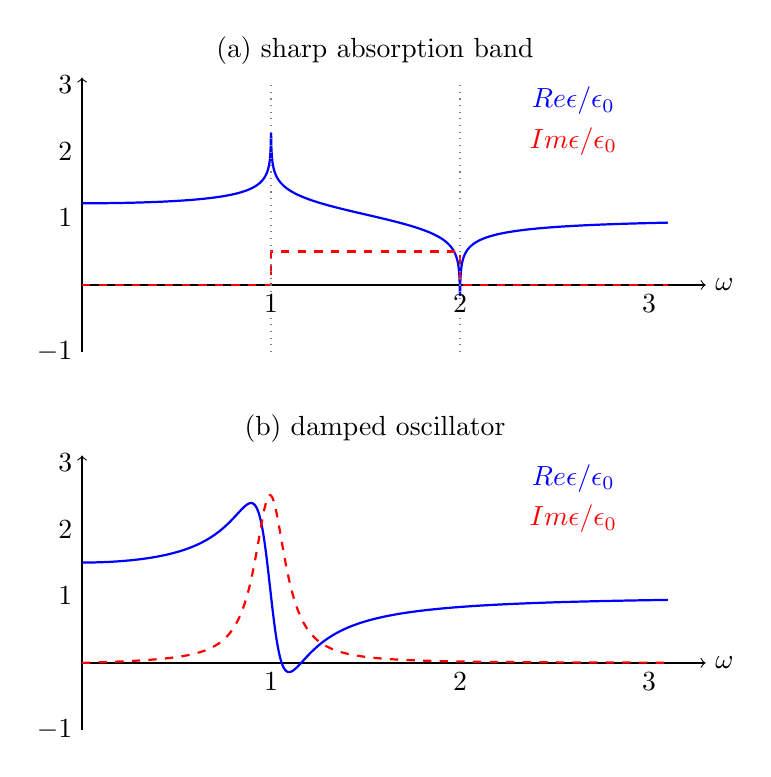
\begin{tikzpicture}[x=2.4cm,y=.85cm]
\begin{scope}[yshift=0.0cm]
\draw[->] (0,-1)--(0,3.1);\draw[->] (0,0)--(3.3,0) node[right] {$\omega$};
\draw[blue,thick] plot coordinates {(0.000000,1.220636) (0.000010,1.220636) (0.000011,1.220636) (0.000013,1.220636) (0.000015,1.220636) (0.000016,1.220636) (0.000019,1.220636) (0.000021,1.220636) (0.000024,1.220636) (0.000027,1.220636) (0.000031,1.220636) (0.000035,1.220636) (0.000039,1.220636) (0.000045,1.220636) (0.000050,1.220636) (0.000057,1.220636) (0.000065,1.220636) (0.000073,1.220636) (0.000083,1.220636) (0.000094,1.220636) (0.000106,1.220636) (0.000120,1.220636) (0.000136,1.220636) (0.000155,1.220636) (0.000175,1.220636) (0.000198,1.220636) (0.000224,1.220636) (0.000254,1.220636) (0.000288,1.220636) (0.000326,1.220636) (0.000369,1.220636) (0.000418,1.220636) (0.000474,1.220636) (0.000536,1.220636) (0.000608,1.220636) (0.000688,1.220636) (0.000779,1.220636) (0.000883,1.220636) (0.001000,1.220636) (0.001132,1.220636) (0.001282,1.220636) (0.001452,1.220636) (0.001644,1.220636) (0.001862,1.220636) (0.002109,1.220636) (0.002389,1.220636) (0.002705,1.220636) (0.003064,1.220637) (0.003470,1.220637) (0.003930,1.220637) (0.004014,1.220638) (0.004451,1.220638) (0.005041,1.220639) (0.005709,1.220639) (0.006465,1.220641) (0.007322,1.220642) (0.008028,1.220643) (0.008293,1.220644) (0.009392,1.220646) (0.010637,1.220649) (0.012042,1.220653) (0.012047,1.220653) (0.013643,1.220658) (0.015452,1.220664) (0.016056,1.220666) (0.017500,1.220672) (0.019819,1.220682) (0.020070,1.220684) (0.022446,1.220696) (0.024084,1.220705) (0.025421,1.220713) (0.028098,1.220730) (0.028790,1.220735) (0.032112,1.220759) (0.032606,1.220763) (0.036127,1.220792) (0.036928,1.220799) (0.040141,1.220828) (0.041822,1.220845) (0.044155,1.220869) (0.047365,1.220904) (0.048169,1.220913) (0.052183,1.220961) (0.053643,1.220980) (0.056197,1.221013) (0.060211,1.221069) (0.060753,1.221077) (0.064225,1.221129) (0.068239,1.221193) (0.068805,1.221202) (0.072253,1.221261) (0.076267,1.221332) (0.077925,1.221363) (0.080281,1.221408) (0.084295,1.221488) (0.088253,1.221570) (0.088309,1.221571) (0.092323,1.221658) (0.096337,1.221750) (0.099950,1.221836) (0.100351,1.221845) (0.104365,1.221945) (0.108380,1.222048) (0.112394,1.222155) (0.116408,1.222267) (0.120422,1.222382) (0.124436,1.222502) (0.128450,1.222626) (0.132464,1.222753) (0.136478,1.222885) (0.140492,1.223021) (0.144506,1.223161) (0.148520,1.223305) (0.152534,1.223454) (0.156548,1.223607) (0.160562,1.223763) (0.164576,1.223924) (0.168590,1.224090) (0.172604,1.224259) (0.176618,1.224433) (0.180633,1.224612) (0.184647,1.224794) (0.188661,1.224981) (0.192675,1.225172) (0.196689,1.225368) (0.200703,1.225568) (0.204717,1.225773) (0.208731,1.225982) (0.212745,1.226196) (0.216759,1.226414) (0.220773,1.226637) (0.224787,1.226865) (0.228801,1.227097) (0.232815,1.227333) (0.236829,1.227575) (0.240843,1.227821) (0.244857,1.228072) (0.248871,1.228328) (0.252886,1.228589) (0.256900,1.228854) (0.260914,1.229125) (0.264928,1.229400) (0.268942,1.229681) (0.272956,1.229966) (0.276970,1.230257) (0.280984,1.230552) (0.284998,1.230853) (0.289012,1.231159) (0.293026,1.231470) (0.297040,1.231787) (0.301054,1.232109) (0.305068,1.232436) (0.309082,1.232769) (0.313096,1.233107) (0.317110,1.233451) (0.321124,1.233800) (0.325139,1.234155) (0.329153,1.234516) (0.333167,1.234882) (0.337181,1.235255) (0.341195,1.235633) (0.345209,1.236017) (0.349223,1.236407) (0.353237,1.236803) (0.357251,1.237206) (0.361265,1.237614) (0.365279,1.238029) (0.369293,1.238450) (0.373307,1.238877) (0.377321,1.239311) (0.381335,1.239752) (0.385349,1.240199) (0.389363,1.240652) (0.393378,1.241113) (0.397392,1.241580) (0.401406,1.242055) (0.405420,1.242536) (0.409434,1.243024) (0.413448,1.243520) (0.417462,1.244023) (0.421476,1.244533) (0.425490,1.245051) (0.429504,1.245576) (0.433518,1.246109) (0.437532,1.246650) (0.441546,1.247198) (0.445560,1.247755) (0.449574,1.248319) (0.453588,1.248892) (0.457602,1.249473) (0.461616,1.250063) (0.465631,1.250661) (0.469645,1.251268) (0.473659,1.251883) (0.477673,1.252508) (0.481687,1.253141) (0.485701,1.253784) (0.489715,1.254436) (0.493729,1.255097) (0.497743,1.255768) (0.501757,1.256449) (0.505771,1.257140) (0.509785,1.257841) (0.513799,1.258552) (0.517813,1.259273) (0.521827,1.260005) (0.525841,1.260748) (0.529855,1.261502) (0.533869,1.262267) (0.537884,1.263043) (0.541898,1.263830) (0.545912,1.264630) (0.549926,1.265441) (0.553940,1.266264) (0.557954,1.267100) (0.561968,1.267948) (0.565982,1.268809) (0.569996,1.269683) (0.574010,1.270570) (0.578024,1.271471) (0.582038,1.272386) (0.586052,1.273314) (0.590066,1.274257) (0.594080,1.275215) (0.598094,1.276187) (0.602108,1.277175) (0.606122,1.278178) (0.610137,1.279197) (0.614151,1.280232) (0.618165,1.281284) (0.622179,1.282352) (0.626193,1.283438) (0.630207,1.284541) (0.634221,1.285663) (0.638235,1.286802) (0.642249,1.287961) (0.646263,1.289139) (0.650277,1.290336) (0.654291,1.291553) (0.658305,1.292792) (0.662319,1.294051) (0.666333,1.295332) (0.670347,1.296635) (0.674361,1.297960) (0.678376,1.299309) (0.682390,1.300682) (0.686404,1.302080) (0.690418,1.303502) (0.694432,1.304950) (0.698446,1.306425) (0.702460,1.307927) (0.706474,1.309457) (0.710488,1.311016) (0.714502,1.312605) (0.718516,1.314223) (0.722530,1.315874) (0.726544,1.317556) (0.730558,1.319272) (0.734572,1.321021) (0.738586,1.322807) (0.742600,1.324628) (0.746614,1.326487) (0.750629,1.328385) (0.754643,1.330324) (0.758657,1.332303) (0.762671,1.334326) (0.766685,1.336392) (0.770699,1.338505) (0.774713,1.340665) (0.778727,1.342875) (0.782741,1.345136) (0.786755,1.347449) (0.790769,1.349818) (0.794783,1.352245) (0.798797,1.354730) (0.802811,1.357278) (0.806825,1.359891) (0.810839,1.362571) (0.814853,1.365321) (0.818867,1.368145) (0.822882,1.371045) (0.826896,1.374026) (0.830910,1.377091) (0.834924,1.380244) (0.838938,1.383490) (0.842952,1.386834) (0.846966,1.390280) (0.850980,1.393834) (0.854994,1.397502) (0.859008,1.401290) (0.863022,1.405206) (0.867036,1.409258) (0.871050,1.413452) (0.875064,1.417800) (0.879078,1.422310) (0.883092,1.426994) (0.887106,1.431864) (0.891120,1.436934) (0.895135,1.442219) (0.899149,1.447735) (0.899550,1.448300) (0.903163,1.453502) (0.907177,1.459541) (0.911191,1.465876) (0.911247,1.465967) (0.915205,1.472535) (0.919219,1.479549) (0.921575,1.483846) (0.923233,1.486954) (0.927247,1.494794) (0.930695,1.501912) (0.931261,1.503117) (0.935275,1.511982) (0.938747,1.520140) (0.939289,1.521458) (0.943303,1.531630) (0.945857,1.538509) (0.947317,1.542599) (0.951331,1.554494) (0.952135,1.556999) (0.955345,1.567472) (0.957678,1.575591) (0.959359,1.581740) (0.962572,1.594268) (0.963373,1.597566) (0.966894,1.613013) (0.967388,1.615313) (0.970710,1.631811) (0.971402,1.635488) (0.974079,1.650647) (0.975416,1.658828) (0.977054,1.669507) (0.979430,1.686466) (0.979681,1.688377) (0.982000,1.707243) (0.983444,1.720281) (0.984048,1.726091) (0.985857,1.744908) (0.987453,1.763680) (0.987458,1.763735) (0.988863,1.782391) (0.990108,1.801026) (0.991207,1.819570) (0.991472,1.824386) (0.992178,1.838005) (0.993035,1.856313) (0.993791,1.874475) (0.994459,1.892471) (0.995049,1.910279) (0.995486,1.924894) (0.995570,1.927875) (0.996030,1.945236) (0.996436,1.962335) (0.996795,1.979145) (0.997111,1.995639) (0.997391,2.011786) (0.997638,2.027557) (0.997856,2.042922) (0.998048,2.057852) (0.998218,2.072315) (0.998368,2.086285) (0.998501,2.099735) (0.998617,2.112639) (0.998721,2.124977) (0.998812,2.136731) (0.998892,2.147886) (0.998964,2.158433) (0.999026,2.168366) (0.999082,2.177684) (0.999131,2.186393) (0.999174,2.194501) (0.999212,2.202021) (0.999246,2.208971) (0.999276,2.215370) (0.999302,2.221244) (0.999325,2.226616) (0.999345,2.231516) (0.999364,2.235972) (0.999380,2.240013) (0.999394,2.243668) (0.999406,2.246967) (0.999417,2.249938) (0.999427,2.252608) (0.999435,2.255004) (0.999443,2.257150) (0.999450,2.259069) (0.999455,2.260782) (0.999461,2.262311) (0.999465,2.263673) (0.999469,2.264886) (0.999473,2.265964) (0.999476,2.266923) (0.999479,2.267774) (0.999481,2.268529) (0.999484,2.269199) (0.999485,2.269793) (0.999487,2.270319) (0.999489,2.270785) (0.999490,2.271198) (0.999500,2.274346)};
\draw[blue,thick] plot coordinates {(1.000500,2.274160) (1.000510,2.271010) (1.000511,2.270597) (1.000513,2.270130) (1.000515,2.269604) (1.000516,2.269010) (1.000519,2.268339) (1.000521,2.267584) (1.000524,2.266732) (1.000527,2.265773) (1.000531,2.264694) (1.000535,2.263480) (1.000539,2.262117) (1.000544,2.260587) (1.000550,2.258871) (1.000557,2.256951) (1.000565,2.254803) (1.000573,2.252406) (1.000583,2.249733) (1.000594,2.246759) (1.000606,2.243457) (1.000620,2.239798) (1.000636,2.235752) (1.000654,2.231292) (1.000675,2.226386) (1.000698,2.221007) (1.000724,2.215126) (1.000754,2.208718) (1.000788,2.201758) (1.000826,2.194226) (1.000869,2.186104) (1.000918,2.177380) (1.000973,2.168043) (1.001036,2.158089) (1.001107,2.147519) (1.001188,2.136336) (1.001279,2.124551) (1.001382,2.112177) (1.001499,2.099231) (1.001631,2.085735) (1.001781,2.071711) (1.001951,2.057186) (1.002144,2.042187) (1.002361,2.026743) (1.002608,2.010881) (1.002888,1.994632) (1.003204,1.978022) (1.003562,1.961080) (1.003968,1.943831) (1.004428,1.926301) (1.004512,1.923289) (1.004949,1.908512) (1.005538,1.890486) (1.006206,1.872243) (1.006962,1.853801) (1.007819,1.835175) (1.008524,1.821295) (1.008789,1.816381) (1.009887,1.797429) (1.011131,1.778332) (1.012536,1.759155) (1.012541,1.759098) (1.014136,1.739734) (1.015944,1.720246) (1.016548,1.714211) (1.017991,1.700637) (1.020309,1.680910) (1.020560,1.678906) (1.022935,1.661064) (1.024572,1.649777) (1.025908,1.641099) (1.028584,1.624946) (1.029276,1.621012) (1.032596,1.603280) (1.033090,1.600796) (1.036608,1.584041) (1.037409,1.580445) (1.040620,1.566722) (1.042301,1.559948) (1.044633,1.550962) (1.047841,1.539295) (1.048645,1.536490) (1.052657,1.523102) (1.054116,1.518468) (1.056669,1.510638) (1.060681,1.498971) (1.061222,1.497451) (1.064693,1.488000) (1.068705,1.477638) (1.069271,1.476222) (1.072717,1.467818) (1.076729,1.458480) (1.078386,1.454753) (1.080741,1.449576) (1.084753,1.441062) (1.088709,1.433015) (1.088765,1.432902) (1.092777,1.425066) (1.096789,1.417524) (1.100400,1.410969) (1.100801,1.410253) (1.104813,1.403232) (1.108825,1.396441) (1.112837,1.389863) (1.116849,1.383484) (1.120861,1.377290) (1.124873,1.371269) (1.128886,1.365408) (1.132898,1.359699) (1.136910,1.354132) (1.140922,1.348698) (1.144934,1.343391) (1.148946,1.338202) (1.152958,1.333125) (1.156970,1.328155) (1.160982,1.323285) (1.164994,1.318511) (1.169006,1.313828) (1.173018,1.309231) (1.177030,1.304716) (1.181042,1.300279) (1.185054,1.295917) (1.189066,1.291626) (1.193078,1.287404) (1.197090,1.283246) (1.201102,1.279151) (1.205114,1.275115) (1.209127,1.271136) (1.213139,1.267213) (1.217151,1.263341) (1.221163,1.259521) (1.225175,1.255748) (1.229187,1.252022) (1.233199,1.248341) (1.237211,1.244703) (1.241223,1.241106) (1.245235,1.237549) (1.249247,1.234031) (1.253259,1.230549) (1.257271,1.227104) (1.261283,1.223692) (1.265295,1.220314) (1.269307,1.216967) (1.273319,1.213651) (1.277331,1.210365) (1.281343,1.207108) (1.285355,1.203878) (1.289367,1.200675) (1.293380,1.197498) (1.297392,1.194345) (1.301404,1.191217) (1.305416,1.188112) (1.309428,1.185029) (1.313440,1.181968) (1.317452,1.178928) (1.321464,1.175908) (1.325476,1.172907) (1.329488,1.169925) (1.333500,1.166962) (1.337512,1.164015) (1.341524,1.161086) (1.345536,1.158173) (1.349548,1.155276) (1.353560,1.152394) (1.357572,1.149526) (1.361584,1.146673) (1.365596,1.143833) (1.369608,1.141006) (1.373620,1.138192) (1.377633,1.135390) (1.381645,1.132599) (1.385657,1.129820) (1.389669,1.127051) (1.393681,1.124292) (1.397693,1.121543) (1.401705,1.118804) (1.405717,1.116073) (1.409729,1.113351) (1.413741,1.110637) (1.417753,1.107931) (1.421765,1.105232) (1.425777,1.102540) (1.429789,1.099855) (1.433801,1.097176) (1.437813,1.094502) (1.441825,1.091835) (1.445837,1.089172) (1.449849,1.086514) (1.453861,1.083860) (1.457873,1.081211) (1.461886,1.078565) (1.465898,1.075923) (1.469910,1.073284) (1.473922,1.070647) (1.477934,1.068013) (1.481946,1.065380) (1.485958,1.062750) (1.489970,1.060121) (1.493982,1.057492) (1.497994,1.054865) (1.502006,1.052238) (1.506018,1.049611) (1.510030,1.046983) (1.514042,1.044355) (1.518054,1.041726) (1.522066,1.039096) (1.526078,1.036464) (1.530090,1.033830) (1.534102,1.031194) (1.538114,1.028555) (1.542127,1.025914) (1.546139,1.023269) (1.550151,1.020620) (1.554163,1.017967) (1.558175,1.015310) (1.562187,1.012648) (1.566199,1.009982) (1.570211,1.007309) (1.574223,1.004631) (1.578235,1.001947) (1.582247,0.999256) (1.586259,0.996558) (1.590271,0.993853) (1.594283,0.991140) (1.598295,0.988420) (1.602307,0.985690) (1.606319,0.982952) (1.610331,0.980204) (1.614343,0.977446) (1.618355,0.974678) (1.622367,0.971900) (1.626380,0.969110) (1.630392,0.966309) (1.634404,0.963495) (1.638416,0.960669) (1.642428,0.957830) (1.646440,0.954977) (1.650452,0.952109) (1.654464,0.949228) (1.658476,0.946330) (1.662488,0.943417) (1.666500,0.940488) (1.670512,0.937541) (1.674524,0.934577) (1.678536,0.931594) (1.682548,0.928592) (1.686560,0.925570) (1.690572,0.922528) (1.694584,0.919465) (1.698596,0.916380) (1.702608,0.913272) (1.706620,0.910140) (1.710633,0.906984) (1.714645,0.903802) (1.718657,0.900595) (1.722669,0.897359) (1.726681,0.894096) (1.730693,0.890804) (1.734705,0.887481) (1.738717,0.884126) (1.742729,0.880739) (1.746741,0.877318) (1.750753,0.873862) (1.754765,0.870369) (1.758777,0.866838) (1.762789,0.863268) (1.766801,0.859657) (1.770813,0.856003) (1.774825,0.852305) (1.778837,0.848561) (1.782849,0.844769) (1.786861,0.840927) (1.790873,0.837032) (1.794886,0.833084) (1.798898,0.829078) (1.802910,0.825014) (1.806922,0.820887) (1.810934,0.816696) (1.814946,0.812438) (1.818958,0.808108) (1.822970,0.803704) (1.826982,0.799223) (1.830994,0.794660) (1.835006,0.790010) (1.839018,0.785271) (1.843030,0.780437) (1.847042,0.775502) (1.851054,0.770461) (1.855066,0.765309) (1.859078,0.760038) (1.863090,0.754642) (1.867102,0.749112) (1.871114,0.743441) (1.875127,0.737619) (1.879139,0.731637) (1.883151,0.725482) (1.887163,0.719143) (1.891175,0.712606) (1.895187,0.705856) (1.899199,0.698876) (1.899600,0.698165) (1.903211,0.691647) (1.907223,0.684148) (1.911235,0.676353) (1.911291,0.676242) (1.915247,0.668237) (1.919259,0.659767) (1.921614,0.654615) (1.923271,0.650906) (1.927283,0.641613) (1.930729,0.633248) (1.931295,0.631838) (1.935307,0.621522) (1.938778,0.612109) (1.939319,0.610596) (1.943331,0.598975) (1.945884,0.591175) (1.947343,0.586558) (1.951355,0.573218) (1.952159,0.570423) (1.955367,0.558793) (1.957699,0.549835) (1.959380,0.543081) (1.962591,0.529398) (1.963392,0.525811) (1.966910,0.509099) (1.967404,0.506621) (1.970724,0.488931) (1.971416,0.485005) (1.974092,0.468885) (1.975428,0.460224) (1.977065,0.448957) (1.979440,0.431146) (1.979691,0.429145) (1.982009,0.409447) (1.983452,0.395892) (1.984056,0.389864) (1.985864,0.370399) (1.987459,0.351056) (1.987464,0.350999) (1.988869,0.331840) (1.990113,0.312759) (1.991211,0.293822) (1.991476,0.288911) (1.992181,0.275040) (1.993038,0.256425) (1.993794,0.237993) (1.994462,0.219758) (1.995051,0.201740) (1.995488,0.186969) (1.995572,0.183958) (1.996032,0.166434) (1.996438,0.149191) (1.996796,0.132253) (1.997112,0.115648) (1.997392,0.099402) (1.997639,0.083544) (1.997856,0.068102) (1.998049,0.053106) (1.998219,0.038583) (1.998369,0.024562) (1.998501,0.011067) (1.998618,-0.001877) (1.998721,-0.014250) (1.998812,-0.026034) (1.998893,-0.037215) (1.998964,-0.047785) (1.999027,-0.057738) (1.999082,-0.067074) (1.999131,-0.075798) (1.999174,-0.083919) (1.999212,-0.091451) (1.999246,-0.098410) (1.999276,-0.104818) (1.999302,-0.110698) (1.999325,-0.116077) (1.999346,-0.120983) (1.999364,-0.125443) (1.999380,-0.129488) (1.999394,-0.133147) (1.999406,-0.136449) (1.999417,-0.139423) (1.999427,-0.142095) (1.999435,-0.144493) (1.999443,-0.146640) (1.999450,-0.148561) (1.999456,-0.150276) (1.999461,-0.151806) (1.999465,-0.153169) (1.999469,-0.154383) (1.999473,-0.155462) (1.999476,-0.156421) (1.999479,-0.157273) (1.999481,-0.158028) (1.999484,-0.158699) (1.999485,-0.159293) (1.999487,-0.159819) (1.999489,-0.160286) (1.999490,-0.160699) (1.999500,-0.163849)};
\draw[blue,thick] plot coordinates {(2.000500,-0.164021) (2.000511,-0.160561) (2.000512,-0.160108) (2.000514,-0.159597) (2.000516,-0.159020) (2.000518,-0.158368) (2.000520,-0.157634) (2.000523,-0.156806) (2.000526,-0.155874) (2.000530,-0.154825) (2.000534,-0.153645) (2.000538,-0.152319) (2.000543,-0.150831) (2.000549,-0.149162) (2.000555,-0.147293) (2.000563,-0.145202) (2.000571,-0.142867) (2.000581,-0.140263) (2.000591,-0.137365) (2.000603,-0.134145) (2.000617,-0.130575) (2.000633,-0.126627) (2.000650,-0.122270) (2.000670,-0.117477) (2.000693,-0.112217) (2.000718,-0.106463) (2.000747,-0.100188) (2.000780,-0.093369) (2.000817,-0.085983) (2.000859,-0.078014) (2.000906,-0.069446) (2.000960,-0.060269) (2.001021,-0.050479) (2.001090,-0.040075) (2.001168,-0.029061) (2.001257,-0.017445) (2.001357,-0.005240) (2.001471,0.007535) (2.001600,0.020861) (2.001745,0.034713) (2.001910,0.049066) (2.002097,0.063892) (2.002309,0.079160) (2.002549,0.094843) (2.002820,0.110908) (2.003128,0.127328) (2.003476,0.144071) (2.003870,0.161110) (2.004317,0.178418) (2.004823,0.195968) (2.004916,0.198980) (2.005396,0.213736) (2.006045,0.231699) (2.006780,0.249834) (2.007612,0.268121) (2.008555,0.286540) (2.009331,0.300234) (2.009623,0.305075) (2.010832,0.323707) (2.012201,0.342420) (2.013747,0.361144) (2.013752,0.361200) (2.015508,0.380032) (2.017497,0.398901) (2.018163,0.404727) (2.019750,0.417796) (2.022302,0.436702) (2.022578,0.438616) (2.025191,0.455605) (2.026994,0.466301) (2.028464,0.474494) (2.031410,0.489673) (2.032170,0.493355) (2.035825,0.509871) (2.036368,0.512174) (2.040241,0.527635) (2.041122,0.530937) (2.044657,0.543475) (2.046506,0.549629) (2.049072,0.557754) (2.052604,0.568234) (2.053488,0.570741) (2.057904,0.582644) (2.059510,0.586736) (2.062319,0.593621) (2.066735,0.603799) (2.067331,0.605118) (2.071151,0.613283) (2.075566,0.622155) (2.076189,0.623361) (2.079982,0.630485) (2.084398,0.638333) (2.086221,0.641444) (2.088813,0.645747) (2.093229,0.652769) (2.097583,0.659346) (2.097645,0.659437) (2.102060,0.665782) (2.106476,0.671832) (2.110450,0.677044) (2.110892,0.677610) (2.115307,0.683139) (2.119723,0.688436) (2.124139,0.693519) (2.128554,0.698404) (2.132970,0.703103) (2.137386,0.707629) (2.141801,0.711993) (2.146217,0.716205) (2.150633,0.720275) (2.155048,0.724210) (2.159464,0.728018) (2.163880,0.731707) (2.168295,0.735283) (2.172711,0.738751) (2.177127,0.742118) (2.181542,0.745388) (2.185958,0.748566) (2.190373,0.751657) (2.194789,0.754665) (2.199205,0.757593) (2.203620,0.760445) (2.208036,0.763225) (2.212452,0.765935) (2.216867,0.768578) (2.221283,0.771158) (2.225699,0.773677) (2.230114,0.776137) (2.234530,0.778540) (2.238946,0.780889) (2.243361,0.783186) (2.247777,0.785433) (2.252193,0.787631) (2.256608,0.789783) (2.261024,0.791889) (2.265440,0.793952) (2.269855,0.795973) (2.274271,0.797954) (2.278687,0.799895) (2.283102,0.801798) (2.287518,0.803665) (2.291934,0.805496) (2.296349,0.807292) (2.300765,0.809055) (2.305181,0.810786) (2.309596,0.812486) (2.314012,0.814155) (2.318428,0.815794) (2.322843,0.817405) (2.327259,0.818988) (2.331675,0.820543) (2.336090,0.822073) (2.340506,0.823577) (2.344922,0.825055) (2.349337,0.826510) (2.353753,0.827941) (2.358169,0.829349) (2.362584,0.830734) (2.367000,0.832098) (2.371416,0.833441) (2.375831,0.834762) (2.380247,0.836064) (2.384663,0.837346) (2.389078,0.838608) (2.393494,0.839852) (2.397910,0.841078) (2.402325,0.842285) (2.406741,0.843475) (2.411157,0.844648) (2.415572,0.845804) (2.419988,0.846944) (2.424404,0.848068) (2.428819,0.849177) (2.433235,0.850270) (2.437651,0.851348) (2.442066,0.852412) (2.446482,0.853461) (2.450898,0.854496) (2.455313,0.855518) (2.459729,0.856526) (2.464145,0.857522) (2.468560,0.858504) (2.472976,0.859474) (2.477392,0.860431) (2.481807,0.861376) (2.486223,0.862310) (2.490639,0.863231) (2.495054,0.864142) (2.499470,0.865041) (2.503886,0.865929) (2.508301,0.866807) (2.512717,0.867674) (2.517133,0.868531) (2.521548,0.869377) (2.525964,0.870214) (2.530380,0.871040) (2.534795,0.871857) (2.539211,0.872665) (2.543627,0.873463) (2.548042,0.874253) (2.552458,0.875033) (2.556873,0.875805) (2.561289,0.876568) (2.565705,0.877322) (2.570120,0.878068) (2.574536,0.878806) (2.578952,0.879536) (2.583367,0.880258) (2.587783,0.880972) (2.592199,0.881679) (2.596614,0.882378) (2.601030,0.883069) (2.605446,0.883754) (2.609861,0.884431) (2.614277,0.885101) (2.618693,0.885764) (2.623108,0.886420) (2.627524,0.887070) (2.631940,0.887713) (2.636355,0.888349) (2.640771,0.888979) (2.645187,0.889603) (2.649602,0.890220) (2.654018,0.890832) (2.658434,0.891437) (2.662849,0.892036) (2.667265,0.892630) (2.671681,0.893218) (2.676096,0.893800) (2.680512,0.894376) (2.684928,0.894947) (2.689343,0.895513) (2.693759,0.896073) (2.698175,0.896628) (2.702590,0.897178) (2.707006,0.897722) (2.711422,0.898262) (2.715837,0.898796) (2.720253,0.899326) (2.724669,0.899851) (2.729084,0.900371) (2.733500,0.900886) (2.737916,0.901397) (2.742331,0.901903) (2.746747,0.902404) (2.751163,0.902901) (2.755578,0.903394) (2.759994,0.903882) (2.764410,0.904366) (2.768825,0.904846) (2.773241,0.905322) (2.777657,0.905793) (2.782072,0.906260) (2.786488,0.906724) (2.790904,0.907183) (2.795319,0.907639) (2.799735,0.908090) (2.804151,0.908538) (2.808566,0.908982) (2.812982,0.909423) (2.817398,0.909859) (2.821813,0.910292) (2.826229,0.910722) (2.830645,0.911148) (2.835060,0.911570) (2.839476,0.911989) (2.843892,0.912405) (2.848307,0.912817) (2.852723,0.913226) (2.857139,0.913632) (2.861554,0.914034) (2.865970,0.914433) (2.870386,0.914829) (2.874801,0.915222) (2.879217,0.915612) (2.883633,0.915998) (2.888048,0.916382) (2.892464,0.916763) (2.896880,0.917140) (2.901295,0.917515) (2.905711,0.917887) (2.910127,0.918256) (2.914542,0.918622) (2.918958,0.918986) (2.923373,0.919347) (2.927789,0.919705) (2.932205,0.920060) (2.936620,0.920412) (2.941036,0.920762) (2.945452,0.921110) (2.949867,0.921455) (2.954283,0.921797) (2.958699,0.922137) (2.963114,0.922474) (2.967530,0.922808) (2.971946,0.923141) (2.976361,0.923471) (2.980777,0.923798) (2.985193,0.924123) (2.989608,0.924446) (2.990050,0.924478) (2.994024,0.924767) (2.998440,0.925085) (3.002855,0.925401) (3.002917,0.925405) (3.007271,0.925714) (3.011687,0.926026) (3.014279,0.926208) (3.016102,0.926335) (3.020518,0.926642) (3.024311,0.926904) (3.024934,0.926947) (3.029349,0.927250) (3.033169,0.927510) (3.033765,0.927551) (3.038181,0.927849) (3.040990,0.928038) (3.042596,0.928146) (3.047012,0.928440) (3.047896,0.928499) (3.051428,0.928733) (3.053994,0.928902) (3.055843,0.929023) (3.059378,0.929254) (3.060259,0.929312) (3.064132,0.929563) (3.064675,0.929598) (3.068330,0.929834) (3.069090,0.929883) (3.072036,0.930072) (3.073506,0.930166) (3.075309,0.930280) (3.077922,0.930446) (3.078198,0.930464) (3.080750,0.930625) (3.082337,0.930725) (3.083003,0.930767) (3.084992,0.930892) (3.086748,0.931002) (3.086753,0.931002) (3.088299,0.931099) (3.089668,0.931184) (3.090877,0.931259) (3.091169,0.931277) (3.091945,0.931326) (3.092888,0.931384) (3.093720,0.931436) (3.094455,0.931481) (3.095104,0.931521) (3.095584,0.931551) (3.095677,0.931556) (3.096183,0.931588) (3.096630,0.931615) (3.097024,0.931639) (3.097372,0.931661) (3.097680,0.931680) (3.097951,0.931696) (3.098191,0.931711) (3.098403,0.931724) (3.098590,0.931736) (3.098755,0.931746) (3.098901,0.931755) (3.099029,0.931763) (3.099143,0.931770) (3.099243,0.931776) (3.099332,0.931781) (3.099410,0.931786) (3.099479,0.931790) (3.099540,0.931794) (3.099594,0.931797) (3.099641,0.931800) (3.099683,0.931803) (3.099720,0.931805) (3.099753,0.931807) (3.099782,0.931809) (3.099807,0.931810) (3.099830,0.931812) (3.099850,0.931813) (3.099867,0.931814) (3.099883,0.931815) (3.099897,0.931816) (3.099909,0.931817) (3.099919,0.931817) (3.099929,0.931818) (3.099937,0.931818) (3.099945,0.931819) (3.099951,0.931819) (3.099957,0.931820) (3.099962,0.931820) (3.099966,0.931820) (3.099970,0.931820) (3.099974,0.931821) (3.099977,0.931821) (3.099980,0.931821) (3.099982,0.931821) (3.099984,0.931821) (3.099986,0.931821) (3.099988,0.931821) (3.099989,0.931822) (3.100000,0.931822)};
\draw[red,dashed,thick] plot coordinates {(0.000000,0.000000) (1.000000,0.000000) (1.000000,0.500000) (2.000000,0.500000) (2.000000,0.000000) (3.100000,0.000000)};
\draw[gray,dotted] (1,-1)--(1,3);
\draw[gray,dotted] (2,-1)--(2,3);
\node at (1.55,3.5) {(a) sharp absorption band};
\node[below] at (1,0) {$1$};\node[left] at (0,1) {$1$};
\node[below] at (2,0) {$2$};\node[left] at (0,2) {$2$};
\node[below] at (3,0) {$3$};\node[left] at (0,3) {$3$};
\node[left] at (0,-1) {$-1$};\node[blue] at (2.6,2.75) {$\operatorname{Re}\epsilon/\epsilon_0$};\node[red] at (2.6,2.15) {$\operatorname{Im}\epsilon/\epsilon_0$};
\end{scope}
\begin{scope}[yshift=-4.8cm]
\draw[->] (0,-1)--(0,3.1);\draw[->] (0,0)--(3.3,0) node[right] {$\omega$};
\draw[blue,thick] plot coordinates {(0.000000,1.500000) (0.003100,1.500005) (0.006200,1.500018) (0.009300,1.500042) (0.012400,1.500074) (0.015500,1.500115) (0.018600,1.500166) (0.021700,1.500226) (0.024800,1.500295) (0.027900,1.500374) (0.031000,1.500462) (0.034100,1.500559) (0.037200,1.500665) (0.040300,1.500781) (0.043400,1.500906) (0.046500,1.501040) (0.049600,1.501184) (0.052700,1.501337) (0.055800,1.501499) (0.058900,1.501671) (0.062000,1.501852) (0.065100,1.502042) (0.068200,1.502242) (0.071300,1.502452) (0.074400,1.502671) (0.077500,1.502899) (0.080600,1.503137) (0.083700,1.503384) (0.086800,1.503642) (0.089900,1.503908) (0.093000,1.504185) (0.096100,1.504471) (0.099200,1.504767) (0.102300,1.505072) (0.105400,1.505387) (0.108500,1.505712) (0.111600,1.506047) (0.114700,1.506392) (0.117800,1.506747) (0.120900,1.507111) (0.124000,1.507486) (0.127100,1.507871) (0.130200,1.508266) (0.133300,1.508670) (0.136400,1.509085) (0.139500,1.509511) (0.142600,1.509946) (0.145700,1.510392) (0.148800,1.510848) (0.151900,1.511315) (0.155000,1.511792) (0.158100,1.512279) (0.161200,1.512778) (0.164300,1.513286) (0.167400,1.513806) (0.170500,1.514336) (0.173600,1.514877) (0.176700,1.515429) (0.179800,1.515991) (0.182900,1.516565) (0.186000,1.517150) (0.189100,1.517746) (0.192200,1.518353) (0.195300,1.518971) (0.198400,1.519601) (0.201500,1.520242) (0.204600,1.520895) (0.207700,1.521559) (0.210800,1.522235) (0.213900,1.522922) (0.217000,1.523622) (0.220100,1.524333) (0.223200,1.525056) (0.226300,1.525791) (0.229400,1.526539) (0.232500,1.527298) (0.235600,1.528070) (0.238700,1.528855) (0.241800,1.529652) (0.244900,1.530461) (0.248000,1.531283) (0.251100,1.532118) (0.254200,1.532966) (0.257300,1.533827) (0.260400,1.534701) (0.263500,1.535589) (0.266600,1.536489) (0.269700,1.537403) (0.272800,1.538331) (0.275900,1.539273) (0.279000,1.540228) (0.282100,1.541197) (0.285200,1.542180) (0.288300,1.543178) (0.291400,1.544189) (0.294500,1.545216) (0.297600,1.546256) (0.300700,1.547312) (0.303800,1.548382) (0.306900,1.549468) (0.310000,1.550568) (0.313100,1.551684) (0.316200,1.552815) (0.319300,1.553962) (0.322400,1.555125) (0.325500,1.556303) (0.328600,1.557498) (0.331700,1.558709) (0.334800,1.559936) (0.337900,1.561180) (0.341000,1.562441) (0.344100,1.563719) (0.347200,1.565013) (0.350300,1.566325) (0.353400,1.567655) (0.356500,1.569002) (0.359600,1.570367) (0.362700,1.571750) (0.365800,1.573152) (0.368900,1.574571) (0.372000,1.576010) (0.375100,1.577468) (0.378200,1.578944) (0.381300,1.580440) (0.384400,1.581956) (0.387500,1.583491) (0.390600,1.585046) (0.393700,1.586622) (0.396800,1.588218) (0.399900,1.589835) (0.403000,1.591473) (0.406100,1.593132) (0.409200,1.594813) (0.412300,1.596516) (0.415400,1.598240) (0.418500,1.599987) (0.421600,1.601757) (0.424700,1.603550) (0.427800,1.605365) (0.430900,1.607205) (0.434000,1.609068) (0.437100,1.610955) (0.440200,1.612867) (0.443300,1.614803) (0.446400,1.616765) (0.449500,1.618752) (0.452600,1.620765) (0.455700,1.622804) (0.458800,1.624869) (0.461900,1.626962) (0.465000,1.629081) (0.468100,1.631228) (0.471200,1.633403) (0.474300,1.635607) (0.477400,1.637839) (0.480500,1.640101) (0.483600,1.642392) (0.486700,1.644713) (0.489800,1.647064) (0.492900,1.649447) (0.496000,1.651860) (0.499100,1.654306) (0.502200,1.656784) (0.505300,1.659294) (0.508400,1.661838) (0.511500,1.664415) (0.514600,1.667027) (0.517700,1.669673) (0.520800,1.672355) (0.523900,1.675073) (0.527000,1.677827) (0.530100,1.680617) (0.533200,1.683445) (0.536300,1.686312) (0.539400,1.689217) (0.542500,1.692161) (0.545600,1.695145) (0.548700,1.698169) (0.551800,1.701235) (0.554900,1.704342) (0.558000,1.707492) (0.561100,1.710685) (0.564200,1.713922) (0.567300,1.717203) (0.570400,1.720529) (0.573500,1.723902) (0.576600,1.727321) (0.579700,1.730787) (0.582800,1.734302) (0.585900,1.737866) (0.589000,1.741480) (0.592100,1.745144) (0.595200,1.748860) (0.598300,1.752628) (0.601400,1.756449) (0.604500,1.760325) (0.607600,1.764255) (0.610700,1.768242) (0.613800,1.772285) (0.616900,1.776386) (0.620000,1.780546) (0.623100,1.784766) (0.626200,1.789046) (0.629300,1.793388) (0.632400,1.797793) (0.635500,1.802262) (0.638600,1.806795) (0.641700,1.811395) (0.644800,1.816062) (0.647900,1.820797) (0.651000,1.825601) (0.654100,1.830476) (0.657200,1.835422) (0.660300,1.840442) (0.663400,1.845535) (0.666500,1.850703) (0.669600,1.855948) (0.672700,1.861271) (0.675800,1.866672) (0.678900,1.872154) (0.682000,1.877717) (0.685100,1.883363) (0.688200,1.889092) (0.691300,1.894907) (0.694400,1.900808) (0.697500,1.906797) (0.700600,1.912874) (0.703700,1.919042) (0.706800,1.925301) (0.709900,1.931653) (0.713000,1.938099) (0.716100,1.944639) (0.719200,1.951276) (0.722300,1.958010) (0.725400,1.964842) (0.728500,1.971773) (0.731600,1.978805) (0.734700,1.985937) (0.737800,1.993172) (0.740900,2.000509) (0.744000,2.007949) (0.747100,2.015493) (0.750200,2.023141) (0.753300,2.030893) (0.756400,2.038750) (0.759500,2.046711) (0.762600,2.054776) (0.765700,2.062945) (0.768800,2.071217) (0.771900,2.079591) (0.775000,2.088065) (0.778100,2.096638) (0.781200,2.105308) (0.784300,2.114073) (0.787400,2.122929) (0.790500,2.131874) (0.793600,2.140904) (0.796700,2.150014) (0.799800,2.159199) (0.802900,2.168453) (0.806000,2.177770) (0.809100,2.187143) (0.812200,2.196562) (0.815300,2.206019) (0.818400,2.215503) (0.821500,2.225002) (0.824600,2.234503) (0.827700,2.243991) (0.830800,2.253451) (0.833900,2.262863) (0.837000,2.272207) (0.840100,2.281463) (0.843200,2.290604) (0.846300,2.299605) (0.849400,2.308434) (0.852500,2.317061) (0.855600,2.325448) (0.858700,2.333556) (0.861800,2.341343) (0.864900,2.348760) (0.868000,2.355756) (0.871100,2.362276) (0.874200,2.368258) (0.877300,2.373636) (0.880400,2.378337) (0.883500,2.382284) (0.886600,2.385393) (0.889700,2.387574) (0.892800,2.388728) (0.895900,2.388753) (0.899000,2.387537) (0.902100,2.384963) (0.905200,2.380906) (0.908300,2.375235) (0.911400,2.367812) (0.914500,2.358495) (0.917600,2.347134) (0.920700,2.333578) (0.923800,2.317673) (0.926900,2.299263) (0.930000,2.278194) (0.933100,2.254314) (0.936200,2.227480) (0.939300,2.197554) (0.942400,2.164413) (0.945500,2.127949) (0.948600,2.088076) (0.951700,2.044728) (0.954800,1.997872) (0.957900,1.947504) (0.961000,1.893658) (0.964100,1.836404) (0.967200,1.775859) (0.970300,1.712180) (0.973400,1.645572) (0.976500,1.576282) (0.979600,1.504602) (0.982700,1.430865) (0.985800,1.355437) (0.988900,1.278717) (0.992000,1.201128) (0.995100,1.123109) (0.998200,1.045107) (1.001300,0.967569) (1.004400,0.890932) (1.007500,0.815618) (1.010600,0.742023) (1.013700,0.670513) (1.016800,0.601416) (1.019900,0.535022) (1.023000,0.471575) (1.026100,0.411275) (1.029200,0.354279) (1.032300,0.300697) (1.035400,0.250598) (1.038500,0.204014) (1.041600,0.160938) (1.044700,0.121333) (1.047800,0.085134) (1.050900,0.052252) (1.054000,0.022577) (1.057100,-0.004015) (1.060200,-0.027660) (1.063300,-0.048505) (1.066400,-0.066701) (1.069500,-0.082401) (1.072600,-0.095763) (1.075700,-0.106939) (1.078800,-0.116082) (1.081900,-0.123340) (1.085000,-0.128855) (1.088100,-0.132764) (1.091200,-0.135198) (1.094300,-0.136281) (1.097400,-0.136131) (1.100500,-0.134858) (1.103600,-0.132565) (1.106700,-0.129349) (1.109800,-0.125300) (1.112900,-0.120502) (1.116000,-0.115031) (1.119100,-0.108960) (1.122200,-0.102354) (1.125300,-0.095274) (1.128400,-0.087777) (1.131500,-0.079913) (1.134600,-0.071728) (1.137700,-0.063267) (1.140800,-0.054568) (1.143900,-0.045667) (1.147000,-0.036596) (1.150100,-0.027385) (1.153200,-0.018060) (1.156300,-0.008647) (1.159400,0.000833) (1.162500,0.010361) (1.165600,0.019917) (1.168700,0.029487) (1.171800,0.039054) (1.174900,0.048607) (1.178000,0.058134) (1.181100,0.067623) (1.184200,0.077066) (1.187300,0.086455) (1.190400,0.095781) (1.193500,0.105039) (1.196600,0.114223) (1.199700,0.123327) (1.202800,0.132348) (1.205900,0.141281) (1.209000,0.150124) (1.212100,0.158873) (1.215200,0.167526) (1.218300,0.176081) (1.221400,0.184537) (1.224500,0.192893) (1.227600,0.201146) (1.230700,0.209298) (1.233800,0.217346) (1.236900,0.225292) (1.240000,0.233134) (1.243100,0.240874) (1.246200,0.248510) (1.249300,0.256045) (1.252400,0.263477) (1.255500,0.270808) (1.258600,0.278039) (1.261700,0.285170) (1.264800,0.292203) (1.267900,0.299137) (1.271000,0.305975) (1.274100,0.312717) (1.277200,0.319364) (1.280300,0.325918) (1.283400,0.332379) (1.286500,0.338750) (1.289600,0.345030) (1.292700,0.351222) (1.295800,0.357326) (1.298900,0.363344) (1.302000,0.369277) (1.305100,0.375126) (1.308200,0.380893) (1.311300,0.386579) (1.314400,0.392185) (1.317500,0.397713) (1.320600,0.403162) (1.323700,0.408536) (1.326800,0.413835) (1.329900,0.419060) (1.333000,0.424213) (1.336100,0.429294) (1.339200,0.434305) (1.342300,0.439247) (1.345400,0.444122) (1.348500,0.448930) (1.351600,0.453672) (1.354700,0.458349) (1.357800,0.462964) (1.360900,0.467516) (1.364000,0.472006) (1.367100,0.476437) (1.370200,0.480808) (1.373300,0.485121) (1.376400,0.489377) (1.379500,0.493577) (1.382600,0.497721) (1.385700,0.501811) (1.388800,0.505847) (1.391900,0.509832) (1.395000,0.513764) (1.398100,0.517646) (1.401200,0.521477) (1.404300,0.525260) (1.407400,0.528995) (1.410500,0.532682) (1.413600,0.536322) (1.416700,0.539917) (1.419800,0.543466) (1.422900,0.546971) (1.426000,0.550433) (1.429100,0.553851) (1.432200,0.557228) (1.435300,0.560563) (1.438400,0.563857) (1.441500,0.567111) (1.444600,0.570326) (1.447700,0.573502) (1.450800,0.576639) (1.453900,0.579739) (1.457000,0.582802) (1.460100,0.585829) (1.463200,0.588820) (1.466300,0.591776) (1.469400,0.594697) (1.472500,0.597584) (1.475600,0.600437) (1.478700,0.603258) (1.481800,0.606046) (1.484900,0.608802) (1.488000,0.611526) (1.491100,0.614220) (1.494200,0.616883) (1.497300,0.619516) (1.500400,0.622119) (1.503500,0.624694) (1.506600,0.627239) (1.509700,0.629757) (1.512800,0.632246) (1.515900,0.634709) (1.519000,0.637144) (1.522100,0.639553) (1.525200,0.641935) (1.528300,0.644292) (1.531400,0.646624) (1.534500,0.648930) (1.537600,0.651212) (1.540700,0.653469) (1.543800,0.655703) (1.546900,0.657913) (1.550000,0.660100) (1.553100,0.662264) (1.556200,0.664405) (1.559300,0.666525) (1.562400,0.668622) (1.565500,0.670698) (1.568600,0.672752) (1.571700,0.674786) (1.574800,0.676798) (1.577900,0.678791) (1.581000,0.680763) (1.584100,0.682716) (1.587200,0.684649) (1.590300,0.686562) (1.593400,0.688457) (1.596500,0.690333) (1.599600,0.692191) (1.602700,0.694030) (1.605800,0.695851) (1.608900,0.697655) (1.612000,0.699441) (1.615100,0.701210) (1.618200,0.702962) (1.621300,0.704697) (1.624400,0.706415) (1.627500,0.708117) (1.630600,0.709803) (1.633700,0.711473) (1.636800,0.713128) (1.639900,0.714767) (1.643000,0.716390) (1.646100,0.717999) (1.649200,0.719592) (1.652300,0.721171) (1.655400,0.722736) (1.658500,0.724286) (1.661600,0.725822) (1.664700,0.727344) (1.667800,0.728852) (1.670900,0.730346) (1.674000,0.731827) (1.677100,0.733295) (1.680200,0.734750) (1.683300,0.736192) (1.686400,0.737621) (1.689500,0.739037) (1.692600,0.740441) (1.695700,0.741833) (1.698800,0.743212) (1.701900,0.744579) (1.705000,0.745935) (1.708100,0.747279) (1.711200,0.748611) (1.714300,0.749932) (1.717400,0.751241) (1.720500,0.752540) (1.723600,0.753827) (1.726700,0.755104) (1.729800,0.756369) (1.732900,0.757624) (1.736000,0.758869) (1.739100,0.760103) (1.742200,0.761327) (1.745300,0.762540) (1.748400,0.763744) (1.751500,0.764938) (1.754600,0.766122) (1.757700,0.767296) (1.760800,0.768461) (1.763900,0.769616) (1.767000,0.770762) (1.770100,0.771898) (1.773200,0.773026) (1.776300,0.774144) (1.779400,0.775254) (1.782500,0.776354) (1.785600,0.777446) (1.788700,0.778529) (1.791800,0.779604) (1.794900,0.780670) (1.798000,0.781728) (1.801100,0.782777) (1.804200,0.783819) (1.807300,0.784852) (1.810400,0.785877) (1.813500,0.786895) (1.816600,0.787904) (1.819700,0.788906) (1.822800,0.789900) (1.825900,0.790887) (1.829000,0.791866) (1.832100,0.792837) (1.835200,0.793802) (1.838300,0.794759) (1.841400,0.795709) (1.844500,0.796651) (1.847600,0.797587) (1.850700,0.798516) (1.853800,0.799438) (1.856900,0.800353) (1.860000,0.801261) (1.863100,0.802163) (1.866200,0.803058) (1.869300,0.803946) (1.872400,0.804828) (1.875500,0.805704) (1.878600,0.806573) (1.881700,0.807436) (1.884800,0.808293) (1.887900,0.809143) (1.891000,0.809988) (1.894100,0.810826) (1.897200,0.811659) (1.900300,0.812485) (1.903400,0.813306) (1.906500,0.814121) (1.909600,0.814930) (1.912700,0.815734) (1.915800,0.816532) (1.918900,0.817324) (1.922000,0.818111) (1.925100,0.818893) (1.928200,0.819669) (1.931300,0.820439) (1.934400,0.821205) (1.937500,0.821965) (1.940600,0.822720) (1.943700,0.823469) (1.946800,0.824214) (1.949900,0.824954) (1.953000,0.825688) (1.956100,0.826418) (1.959200,0.827143) (1.962300,0.827862) (1.965400,0.828577) (1.968500,0.829288) (1.971600,0.829993) (1.974700,0.830694) (1.977800,0.831390) (1.980900,0.832082) (1.984000,0.832769) (1.987100,0.833452) (1.990200,0.834130) (1.993300,0.834803) (1.996400,0.835473) (1.999500,0.836138) (2.002600,0.836798) (2.005700,0.837455) (2.008800,0.838107) (2.011900,0.838755) (2.015000,0.839398) (2.018100,0.840038) (2.021200,0.840674) (2.024300,0.841305) (2.027400,0.841933) (2.030500,0.842556) (2.033600,0.843176) (2.036700,0.843792) (2.039800,0.844403) (2.042900,0.845011) (2.046000,0.845616) (2.049100,0.846216) (2.052200,0.846813) (2.055300,0.847406) (2.058400,0.847995) (2.061500,0.848581) (2.064600,0.849163) (2.067700,0.849741) (2.070800,0.850316) (2.073900,0.850888) (2.077000,0.851456) (2.080100,0.852020) (2.083200,0.852581) (2.086300,0.853139) (2.089400,0.853693) (2.092500,0.854244) (2.095600,0.854792) (2.098700,0.855336) (2.101800,0.855877) (2.104900,0.856415) (2.108000,0.856950) (2.111100,0.857481) (2.114200,0.858010) (2.117300,0.858535) (2.120400,0.859057) (2.123500,0.859576) (2.126600,0.860092) (2.129700,0.860605) (2.132800,0.861115) (2.135900,0.861622) (2.139000,0.862126) (2.142100,0.862628) (2.145200,0.863126) (2.148300,0.863621) (2.151400,0.864114) (2.154500,0.864603) (2.157600,0.865090) (2.160700,0.865574) (2.163800,0.866056) (2.166900,0.866534) (2.170000,0.867010) (2.173100,0.867483) (2.176200,0.867954) (2.179300,0.868422) (2.182400,0.868887) (2.185500,0.869349) (2.188600,0.869809) (2.191700,0.870267) (2.194800,0.870722) (2.197900,0.871174) (2.201000,0.871624) (2.204100,0.872071) (2.207200,0.872516) (2.210300,0.872958) (2.213400,0.873398) (2.216500,0.873836) (2.219600,0.874271) (2.222700,0.874704) (2.225800,0.875134) (2.228900,0.875562) (2.232000,0.875988) (2.235100,0.876411) (2.238200,0.876833) (2.241300,0.877251) (2.244400,0.877668) (2.247500,0.878082) (2.250600,0.878494) (2.253700,0.878904) (2.256800,0.879312) (2.259900,0.879718) (2.263000,0.880121) (2.266100,0.880522) (2.269200,0.880921) (2.272300,0.881318) (2.275400,0.881713) (2.278500,0.882106) (2.281600,0.882497) (2.284700,0.882886) (2.287800,0.883272) (2.290900,0.883657) (2.294000,0.884040) (2.297100,0.884420) (2.300200,0.884799) (2.303300,0.885176) (2.306400,0.885551) (2.309500,0.885923) (2.312600,0.886294) (2.315700,0.886663) (2.318800,0.887030) (2.321900,0.887396) (2.325000,0.887759) (2.328100,0.888121) (2.331200,0.888480) (2.334300,0.888838) (2.337400,0.889194) (2.340500,0.889548) (2.343600,0.889901) (2.346700,0.890252) (2.349800,0.890601) (2.352900,0.890948) (2.356000,0.891293) (2.359100,0.891637) (2.362200,0.891979) (2.365300,0.892319) (2.368400,0.892658) (2.371500,0.892995) (2.374600,0.893330) (2.377700,0.893663) (2.380800,0.893995) (2.383900,0.894326) (2.387000,0.894654) (2.390100,0.894982) (2.393200,0.895307) (2.396300,0.895631) (2.399400,0.895953) (2.402500,0.896274) (2.405600,0.896593) (2.408700,0.896911) (2.411800,0.897227) (2.414900,0.897541) (2.418000,0.897854) (2.421100,0.898166) (2.424200,0.898476) (2.427300,0.898785) (2.430400,0.899092) (2.433500,0.899397) (2.436600,0.899702) (2.439700,0.900004) (2.442800,0.900306) (2.445900,0.900605) (2.449000,0.900904) (2.452100,0.901201) (2.455200,0.901497) (2.458300,0.901791) (2.461400,0.902084) (2.464500,0.902375) (2.467600,0.902665) (2.470700,0.902954) (2.473800,0.903241) (2.476900,0.903527) (2.480000,0.903812) (2.483100,0.904096) (2.486200,0.904378) (2.489300,0.904659) (2.492400,0.904938) (2.495500,0.905216) (2.498600,0.905493) (2.501700,0.905769) (2.504800,0.906043) (2.507900,0.906317) (2.511000,0.906589) (2.514100,0.906859) (2.517200,0.907129) (2.520300,0.907397) (2.523400,0.907664) (2.526500,0.907930) (2.529600,0.908194) (2.532700,0.908458) (2.535800,0.908720) (2.538900,0.908981) (2.542000,0.909241) (2.545100,0.909500) (2.548200,0.909757) (2.551300,0.910014) (2.554400,0.910269) (2.557500,0.910523) (2.560600,0.910776) (2.563700,0.911028) (2.566800,0.911279) (2.569900,0.911528) (2.573000,0.911777) (2.576100,0.912024) (2.579200,0.912271) (2.582300,0.912516) (2.585400,0.912760) (2.588500,0.913003) (2.591600,0.913245) (2.594700,0.913487) (2.597800,0.913727) (2.600900,0.913965) (2.604000,0.914203) (2.607100,0.914440) (2.610200,0.914676) (2.613300,0.914911) (2.616400,0.915145) (2.619500,0.915378) (2.622600,0.915609) (2.625700,0.915840) (2.628800,0.916070) (2.631900,0.916299) (2.635000,0.916527) (2.638100,0.916754) (2.641200,0.916980) (2.644300,0.917205) (2.647400,0.917429) (2.650500,0.917652) (2.653600,0.917874) (2.656700,0.918095) (2.659800,0.918316) (2.662900,0.918535) (2.666000,0.918753) (2.669100,0.918971) (2.672200,0.919188) (2.675300,0.919403) (2.678400,0.919618) (2.681500,0.919832) (2.684600,0.920045) (2.687700,0.920257) (2.690800,0.920468) (2.693900,0.920679) (2.697000,0.920888) (2.700100,0.921097) (2.703200,0.921305) (2.706300,0.921512) (2.709400,0.921718) (2.712500,0.921923) (2.715600,0.922128) (2.718700,0.922331) (2.721800,0.922534) (2.724900,0.922736) (2.728000,0.922937) (2.731100,0.923137) (2.734200,0.923337) (2.737300,0.923535) (2.740400,0.923733) (2.743500,0.923930) (2.746600,0.924127) (2.749700,0.924322) (2.752800,0.924517) (2.755900,0.924711) (2.759000,0.924904) (2.762100,0.925096) (2.765200,0.925288) (2.768300,0.925479) (2.771400,0.925669) (2.774500,0.925858) (2.777600,0.926047) (2.780700,0.926234) (2.783800,0.926422) (2.786900,0.926608) (2.790000,0.926794) (2.793100,0.926978) (2.796200,0.927163) (2.799300,0.927346) (2.802400,0.927529) (2.805500,0.927711) (2.808600,0.927892) (2.811700,0.928073) (2.814800,0.928252) (2.817900,0.928432) (2.821000,0.928610) (2.824100,0.928788) (2.827200,0.928965) (2.830300,0.929141) (2.833400,0.929317) (2.836500,0.929492) (2.839600,0.929667) (2.842700,0.929840) (2.845800,0.930013) (2.848900,0.930186) (2.852000,0.930357) (2.855100,0.930528) (2.858200,0.930699) (2.861300,0.930869) (2.864400,0.931038) (2.867500,0.931206) (2.870600,0.931374) (2.873700,0.931541) (2.876800,0.931708) (2.879900,0.931874) (2.883000,0.932039) (2.886100,0.932204) (2.889200,0.932368) (2.892300,0.932531) (2.895400,0.932694) (2.898500,0.932856) (2.901600,0.933018) (2.904700,0.933179) (2.907800,0.933339) (2.910900,0.933499) (2.914000,0.933658) (2.917100,0.933817) (2.920200,0.933975) (2.923300,0.934132) (2.926400,0.934289) (2.929500,0.934446) (2.932600,0.934601) (2.935700,0.934756) (2.938800,0.934911) (2.941900,0.935065) (2.945000,0.935218) (2.948100,0.935371) (2.951200,0.935524) (2.954300,0.935675) (2.957400,0.935827) (2.960500,0.935977) (2.963600,0.936127) (2.966700,0.936277) (2.969800,0.936426) (2.972900,0.936574) (2.976000,0.936722) (2.979100,0.936870) (2.982200,0.937016) (2.985300,0.937163) (2.988400,0.937309) (2.991500,0.937454) (2.994600,0.937599) (2.997700,0.937743) (3.000800,0.937887) (3.003900,0.938030) (3.007000,0.938173) (3.010100,0.938315) (3.013200,0.938456) (3.016300,0.938598) (3.019400,0.938738) (3.022500,0.938878) (3.025600,0.939018) (3.028700,0.939157) (3.031800,0.939296) (3.034900,0.939434) (3.038000,0.939572) (3.041100,0.939709) (3.044200,0.939846) (3.047300,0.939982) (3.050400,0.940118) (3.053500,0.940253) (3.056600,0.940388) (3.059700,0.940523) (3.062800,0.940656) (3.065900,0.940790) (3.069000,0.940923) (3.072100,0.941055) (3.075200,0.941187) (3.078300,0.941319) (3.081400,0.941450) (3.084500,0.941581) (3.087600,0.941711) (3.090700,0.941841) (3.093800,0.941970) (3.096900,0.942099) (3.100000,0.942228)};
\draw[red,dashed,thick] plot coordinates {(0.000000,0.000000) (0.003100,0.000310) (0.006200,0.000620) (0.009300,0.000930) (0.012400,0.001240) (0.015500,0.001551) (0.018600,0.001861) (0.021700,0.002172) (0.024800,0.002483) (0.027900,0.002794) (0.031000,0.003106) (0.034100,0.003418) (0.037200,0.003730) (0.040300,0.004043) (0.043400,0.004356) (0.046500,0.004670) (0.049600,0.004984) (0.052700,0.005299) (0.055800,0.005614) (0.058900,0.005930) (0.062000,0.006247) (0.065100,0.006564) (0.068200,0.006883) (0.071300,0.007202) (0.074400,0.007521) (0.077500,0.007842) (0.080600,0.008164) (0.083700,0.008486) (0.086800,0.008810) (0.089900,0.009134) (0.093000,0.009460) (0.096100,0.009786) (0.099200,0.010114) (0.102300,0.010443) (0.105400,0.010773) (0.108500,0.011105) (0.111600,0.011437) (0.114700,0.011772) (0.117800,0.012107) (0.120900,0.012444) (0.124000,0.012782) (0.127100,0.013122) (0.130200,0.013463) (0.133300,0.013806) (0.136400,0.014151) (0.139500,0.014497) (0.142600,0.014846) (0.145700,0.015195) (0.148800,0.015547) (0.151900,0.015901) (0.155000,0.016256) (0.158100,0.016614) (0.161200,0.016973) (0.164300,0.017335) (0.167400,0.017698) (0.170500,0.018064) (0.173600,0.018432) (0.176700,0.018802) (0.179800,0.019175) (0.182900,0.019550) (0.186000,0.019927) (0.189100,0.020307) (0.192200,0.020690) (0.195300,0.021075) (0.198400,0.021463) (0.201500,0.021853) (0.204600,0.022246) (0.207700,0.022642) (0.210800,0.023041) (0.213900,0.023443) (0.217000,0.023848) (0.220100,0.024256) (0.223200,0.024667) (0.226300,0.025082) (0.229400,0.025499) (0.232500,0.025921) (0.235600,0.026345) (0.238700,0.026773) (0.241800,0.027205) (0.244900,0.027640) (0.248000,0.028079) (0.251100,0.028521) (0.254200,0.028968) (0.257300,0.029418) (0.260400,0.029873) (0.263500,0.030332) (0.266600,0.030794) (0.269700,0.031261) (0.272800,0.031733) (0.275900,0.032209) (0.279000,0.032689) (0.282100,0.033174) (0.285200,0.033664) (0.288300,0.034159) (0.291400,0.034658) (0.294500,0.035163) (0.297600,0.035673) (0.300700,0.036187) (0.303800,0.036708) (0.306900,0.037233) (0.310000,0.037764) (0.313100,0.038301) (0.316200,0.038844) (0.319300,0.039392) (0.322400,0.039947) (0.325500,0.040507) (0.328600,0.041074) (0.331700,0.041647) (0.334800,0.042227) (0.337900,0.042813) (0.341000,0.043406) (0.344100,0.044006) (0.347200,0.044612) (0.350300,0.045226) (0.353400,0.045848) (0.356500,0.046477) (0.359600,0.047113) (0.362700,0.047757) (0.365800,0.048409) (0.368900,0.049070) (0.372000,0.049738) (0.375100,0.050415) (0.378200,0.051101) (0.381300,0.051795) (0.384400,0.052498) (0.387500,0.053210) (0.390600,0.053932) (0.393700,0.054663) (0.396800,0.055404) (0.399900,0.056155) (0.403000,0.056916) (0.406100,0.057688) (0.409200,0.058470) (0.412300,0.059263) (0.415400,0.060067) (0.418500,0.060882) (0.421600,0.061709) (0.424700,0.062547) (0.427800,0.063398) (0.430900,0.064260) (0.434000,0.065136) (0.437100,0.066024) (0.440200,0.066925) (0.443300,0.067840) (0.446400,0.068768) (0.449500,0.069711) (0.452600,0.070668) (0.455700,0.071639) (0.458800,0.072625) (0.461900,0.073627) (0.465000,0.074645) (0.468100,0.075678) (0.471200,0.076728) (0.474300,0.077794) (0.477400,0.078878) (0.480500,0.079979) (0.483600,0.081099) (0.486700,0.082236) (0.489800,0.083393) (0.492900,0.084568) (0.496000,0.085764) (0.499100,0.086979) (0.502200,0.088216) (0.505300,0.089473) (0.508400,0.090753) (0.511500,0.092054) (0.514600,0.093378) (0.517700,0.094726) (0.520800,0.096097) (0.523900,0.097493) (0.527000,0.098914) (0.530100,0.100361) (0.533200,0.101834) (0.536300,0.103335) (0.539400,0.104863) (0.542500,0.106419) (0.545600,0.108005) (0.548700,0.109621) (0.551800,0.111267) (0.554900,0.112945) (0.558000,0.114656) (0.561100,0.116399) (0.564200,0.118177) (0.567300,0.119990) (0.570400,0.121839) (0.573500,0.123725) (0.576600,0.125649) (0.579700,0.127612) (0.582800,0.129615) (0.585900,0.131659) (0.589000,0.133745) (0.592100,0.135876) (0.595200,0.138050) (0.598300,0.140271) (0.601400,0.142540) (0.604500,0.144857) (0.607600,0.147224) (0.610700,0.149643) (0.613800,0.152115) (0.616900,0.154642) (0.620000,0.157225) (0.623100,0.159866) (0.626200,0.162567) (0.629300,0.165329) (0.632400,0.168155) (0.635500,0.171046) (0.638600,0.174005) (0.641700,0.177033) (0.644800,0.180132) (0.647900,0.183306) (0.651000,0.186556) (0.654100,0.189884) (0.657200,0.193294) (0.660300,0.196787) (0.663400,0.200367) (0.666500,0.204036) (0.669600,0.207798) (0.672700,0.211654) (0.675800,0.215610) (0.678900,0.219667) (0.682000,0.223829) (0.685100,0.228100) (0.688200,0.232483) (0.691300,0.236983) (0.694400,0.241603) (0.697500,0.246348) (0.700600,0.251222) (0.703700,0.256229) (0.706800,0.261374) (0.709900,0.266663) (0.713000,0.272100) (0.716100,0.277691) (0.719200,0.283441) (0.722300,0.289356) (0.725400,0.295443) (0.728500,0.301707) (0.731600,0.308155) (0.734700,0.314795) (0.737800,0.321633) (0.740900,0.328677) (0.744000,0.335935) (0.747100,0.343415) (0.750200,0.351125) (0.753300,0.359076) (0.756400,0.367275) (0.759500,0.375734) (0.762600,0.384461) (0.765700,0.393469) (0.768800,0.402767) (0.771900,0.412369) (0.775000,0.422285) (0.778100,0.432529) (0.781200,0.443114) (0.784300,0.454054) (0.787400,0.465364) (0.790500,0.477059) (0.793600,0.489154) (0.796700,0.501666) (0.799800,0.514613) (0.802900,0.528013) (0.806000,0.541884) (0.809100,0.556246) (0.812200,0.571119) (0.815300,0.586525) (0.818400,0.602485) (0.821500,0.619023) (0.824600,0.636163) (0.827700,0.653928) (0.830800,0.672345) (0.833900,0.691440) (0.837000,0.711241) (0.840100,0.731774) (0.843200,0.753070) (0.846300,0.775157) (0.849400,0.798065) (0.852500,0.821826) (0.855600,0.846471) (0.858700,0.872030) (0.861800,0.898535) (0.864900,0.926018) (0.868000,0.954510) (0.871100,0.984041) (0.874200,1.014641) (0.877300,1.046337) (0.880400,1.079156) (0.883500,1.113121) (0.886600,1.148254) (0.889700,1.184571) (0.892800,1.222086) (0.895900,1.260806) (0.899000,1.300733) (0.902100,1.341859) (0.905200,1.384171) (0.908300,1.427645) (0.911400,1.472246) (0.914500,1.517924) (0.917600,1.564620) (0.920700,1.612255) (0.923800,1.660736) (0.926900,1.709950) (0.930000,1.759764) (0.933100,1.810023) (0.936200,1.860553) (0.939300,1.911154) (0.942400,1.961603) (0.945500,2.011654) (0.948600,2.061040) (0.951700,2.109470) (0.954800,2.156635) (0.957900,2.202211) (0.961000,2.245858) (0.964100,2.287232) (0.967200,2.325984) (0.970300,2.361768) (0.973400,2.394249) (0.976500,2.423108) (0.979600,2.448051) (0.982700,2.468816) (0.985800,2.485176) (0.988900,2.496950) (0.992000,2.504006) (0.995100,2.506263) (0.998200,2.503695) (1.001300,2.496333) (1.004400,2.484260) (1.007500,2.467612) (1.010600,2.446576) (1.013700,2.421378) (1.016800,2.392285) (1.019900,2.359593) (1.023000,2.323621) (1.026100,2.284707) (1.029200,2.243195) (1.032300,2.199435) (1.035400,2.153773) (1.038500,2.106544) (1.041600,2.058074) (1.044700,2.008670) (1.047800,1.958621) (1.050900,1.908192) (1.054000,1.857629) (1.057100,1.807152) (1.060200,1.756958) (1.063300,1.707223) (1.066400,1.658098) (1.069500,1.609715) (1.072600,1.562184) (1.075700,1.515600) (1.078800,1.470037) (1.081900,1.425557) (1.085000,1.382206) (1.088100,1.340019) (1.091200,1.299019) (1.094300,1.259220) (1.097400,1.220628) (1.100500,1.183240) (1.103600,1.147049) (1.106700,1.112042) (1.109800,1.078201) (1.112900,1.045504) (1.116000,1.013929) (1.119100,0.983448) (1.122200,0.954034) (1.125300,0.925657) (1.128400,0.898286) (1.131500,0.871891) (1.134600,0.846440) (1.137700,0.821901) (1.140800,0.798243) (1.143900,0.775436) (1.147000,0.753448) (1.150100,0.732250) (1.153200,0.711811) (1.156300,0.692104) (1.159400,0.673100) (1.162500,0.654772) (1.165600,0.637094) (1.168700,0.620040) (1.171800,0.603586) (1.174900,0.587708) (1.178000,0.572383) (1.181100,0.557589) (1.184200,0.543305) (1.187300,0.529510) (1.190400,0.516186) (1.193500,0.503313) (1.196600,0.490873) (1.199700,0.478849) (1.202800,0.467225) (1.205900,0.455985) (1.209000,0.445113) (1.212100,0.434595) (1.215200,0.424417) (1.218300,0.414567) (1.221400,0.405030) (1.224500,0.395796) (1.227600,0.386852) (1.230700,0.378187) (1.233800,0.369790) (1.236900,0.361652) (1.240000,0.353762) (1.243100,0.346112) (1.246200,0.338691) (1.249300,0.331493) (1.252400,0.324507) (1.255500,0.317727) (1.258600,0.311145) (1.261700,0.304754) (1.264800,0.298547) (1.267900,0.292517) (1.271000,0.286658) (1.274100,0.280964) (1.277200,0.275429) (1.280300,0.270047) (1.283400,0.264813) (1.286500,0.259723) (1.289600,0.254770) (1.292700,0.249951) (1.295800,0.245260) (1.298900,0.240694) (1.302000,0.236248) (1.305100,0.231918) (1.308200,0.227700) (1.311300,0.223591) (1.314400,0.219588) (1.317500,0.215686) (1.320600,0.211882) (1.323700,0.208173) (1.326800,0.204557) (1.329900,0.201030) (1.333000,0.197589) (1.336100,0.194232) (1.339200,0.190956) (1.342300,0.187759) (1.345400,0.184638) (1.348500,0.181591) (1.351600,0.178616) (1.354700,0.175710) (1.357800,0.172871) (1.360900,0.170098) (1.364000,0.167388) (1.367100,0.164740) (1.370200,0.162151) (1.373300,0.159621) (1.376400,0.157147) (1.379500,0.154728) (1.382600,0.152362) (1.385700,0.150047) (1.388800,0.147783) (1.391900,0.145568) (1.395000,0.143400) (1.398100,0.141278) (1.401200,0.139201) (1.404300,0.137168) (1.407400,0.135177) (1.410500,0.133228) (1.413600,0.131319) (1.416700,0.129449) (1.419800,0.127617) (1.422900,0.125822) (1.426000,0.124063) (1.429100,0.122340) (1.432200,0.120651) (1.435300,0.118995) (1.438400,0.117372) (1.441500,0.115780) (1.444600,0.114219) (1.447700,0.112689) (1.450800,0.111188) (1.453900,0.109715) (1.457000,0.108270) (1.460100,0.106853) (1.463200,0.105462) (1.466300,0.104097) (1.469400,0.102758) (1.472500,0.101443) (1.475600,0.100152) (1.478700,0.098885) (1.481800,0.097641) (1.484900,0.096419) (1.488000,0.095219) (1.491100,0.094041) (1.494200,0.092883) (1.497300,0.091746) (1.500400,0.090629) (1.503500,0.089531) (1.506600,0.088452) (1.509700,0.087392) (1.512800,0.086350) (1.515900,0.085326) (1.519000,0.084319) (1.522100,0.083330) (1.525200,0.082356) (1.528300,0.081400) (1.531400,0.080459) (1.534500,0.079534) (1.537600,0.078624) (1.540700,0.077728) (1.543800,0.076848) (1.546900,0.075982) (1.550000,0.075129) (1.553100,0.074291) (1.556200,0.073466) (1.559300,0.072654) (1.562400,0.071854) (1.565500,0.071068) (1.568600,0.070294) (1.571700,0.069531) (1.574800,0.068781) (1.577900,0.068042) (1.581000,0.067315) (1.584100,0.066599) (1.587200,0.065893) (1.590300,0.065198) (1.593400,0.064514) (1.596500,0.063840) (1.599600,0.063176) (1.602700,0.062522) (1.605800,0.061878) (1.608900,0.061243) (1.612000,0.060618) (1.615100,0.060001) (1.618200,0.059394) (1.621300,0.058795) (1.624400,0.058205) (1.627500,0.057624) (1.630600,0.057051) (1.633700,0.056486) (1.636800,0.055929) (1.639900,0.055379) (1.643000,0.054838) (1.646100,0.054304) (1.649200,0.053777) (1.652300,0.053258) (1.655400,0.052746) (1.658500,0.052241) (1.661600,0.051743) (1.664700,0.051252) (1.667800,0.050767) (1.670900,0.050289) (1.674000,0.049817) (1.677100,0.049352) (1.680200,0.048893) (1.683300,0.048439) (1.686400,0.047992) (1.689500,0.047551) (1.692600,0.047116) (1.695700,0.046686) (1.698800,0.046262) (1.701900,0.045843) (1.705000,0.045430) (1.708100,0.045022) (1.711200,0.044619) (1.714300,0.044222) (1.717400,0.043829) (1.720500,0.043442) (1.723600,0.043059) (1.726700,0.042681) (1.729800,0.042308) (1.732900,0.041940) (1.736000,0.041576) (1.739100,0.041216) (1.742200,0.040861) (1.745300,0.040511) (1.748400,0.040164) (1.751500,0.039822) (1.754600,0.039484) (1.757700,0.039150) (1.760800,0.038820) (1.763900,0.038494) (1.767000,0.038172) (1.770100,0.037854) (1.773200,0.037540) (1.776300,0.037229) (1.779400,0.036922) (1.782500,0.036619) (1.785600,0.036319) (1.788700,0.036022) (1.791800,0.035729) (1.794900,0.035440) (1.798000,0.035153) (1.801100,0.034870) (1.804200,0.034591) (1.807300,0.034314) (1.810400,0.034041) (1.813500,0.033770) (1.816600,0.033503) (1.819700,0.033239) (1.822800,0.032978) (1.825900,0.032719) (1.829000,0.032464) (1.832100,0.032211) (1.835200,0.031961) (1.838300,0.031714) (1.841400,0.031470) (1.844500,0.031228) (1.847600,0.030989) (1.850700,0.030752) (1.853800,0.030518) (1.856900,0.030287) (1.860000,0.030058) (1.863100,0.029832) (1.866200,0.029608) (1.869300,0.029386) (1.872400,0.029167) (1.875500,0.028950) (1.878600,0.028735) (1.881700,0.028522) (1.884800,0.028312) (1.887900,0.028104) (1.891000,0.027898) (1.894100,0.027695) (1.897200,0.027493) (1.900300,0.027293) (1.903400,0.027096) (1.906500,0.026900) (1.909600,0.026707) (1.912700,0.026515) (1.915800,0.026326) (1.918900,0.026138) (1.922000,0.025952) (1.925100,0.025769) (1.928200,0.025587) (1.931300,0.025406) (1.934400,0.025228) (1.937500,0.025051) (1.940600,0.024876) (1.943700,0.024703) (1.946800,0.024532) (1.949900,0.024362) (1.953000,0.024194) (1.956100,0.024027) (1.959200,0.023862) (1.962300,0.023699) (1.965400,0.023537) (1.968500,0.023377) (1.971600,0.023219) (1.974700,0.023062) (1.977800,0.022906) (1.980900,0.022752) (1.984000,0.022599) (1.987100,0.022448) (1.990200,0.022298) (1.993300,0.022150) (1.996400,0.022003) (1.999500,0.021857) (2.002600,0.021713) (2.005700,0.021570) (2.008800,0.021429) (2.011900,0.021289) (2.015000,0.021150) (2.018100,0.021012) (2.021200,0.020875) (2.024300,0.020740) (2.027400,0.020606) (2.030500,0.020474) (2.033600,0.020342) (2.036700,0.020212) (2.039800,0.020083) (2.042900,0.019955) (2.046000,0.019828) (2.049100,0.019702) (2.052200,0.019578) (2.055300,0.019454) (2.058400,0.019332) (2.061500,0.019211) (2.064600,0.019090) (2.067700,0.018971) (2.070800,0.018853) (2.073900,0.018736) (2.077000,0.018620) (2.080100,0.018505) (2.083200,0.018391) (2.086300,0.018278) (2.089400,0.018166) (2.092500,0.018055) (2.095600,0.017945) (2.098700,0.017835) (2.101800,0.017727) (2.104900,0.017620) (2.108000,0.017513) (2.111100,0.017408) (2.114200,0.017303) (2.117300,0.017199) (2.120400,0.017097) (2.123500,0.016994) (2.126600,0.016893) (2.129700,0.016793) (2.132800,0.016694) (2.135900,0.016595) (2.139000,0.016497) (2.142100,0.016400) (2.145200,0.016304) (2.148300,0.016208) (2.151400,0.016114) (2.154500,0.016020) (2.157600,0.015927) (2.160700,0.015834) (2.163800,0.015743) (2.166900,0.015652) (2.170000,0.015562) (2.173100,0.015473) (2.176200,0.015384) (2.179300,0.015296) (2.182400,0.015209) (2.185500,0.015122) (2.188600,0.015036) (2.191700,0.014951) (2.194800,0.014867) (2.197900,0.014783) (2.201000,0.014700) (2.204100,0.014617) (2.207200,0.014535) (2.210300,0.014454) (2.213400,0.014373) (2.216500,0.014293) (2.219600,0.014214) (2.222700,0.014135) (2.225800,0.014057) (2.228900,0.013980) (2.232000,0.013903) (2.235100,0.013827) (2.238200,0.013751) (2.241300,0.013676) (2.244400,0.013601) (2.247500,0.013527) (2.250600,0.013454) (2.253700,0.013381) (2.256800,0.013309) (2.259900,0.013237) (2.263000,0.013165) (2.266100,0.013095) (2.269200,0.013025) (2.272300,0.012955) (2.275400,0.012886) (2.278500,0.012817) (2.281600,0.012749) (2.284700,0.012682) (2.287800,0.012614) (2.290900,0.012548) (2.294000,0.012482) (2.297100,0.012416) (2.300200,0.012351) (2.303300,0.012286) (2.306400,0.012222) (2.309500,0.012158) (2.312600,0.012095) (2.315700,0.012032) (2.318800,0.011970) (2.321900,0.011908) (2.325000,0.011847) (2.328100,0.011786) (2.331200,0.011725) (2.334300,0.011665) (2.337400,0.011605) (2.340500,0.011546) (2.343600,0.011487) (2.346700,0.011429) (2.349800,0.011371) (2.352900,0.011313) (2.356000,0.011256) (2.359100,0.011199) (2.362200,0.011143) (2.365300,0.011087) (2.368400,0.011031) (2.371500,0.010976) (2.374600,0.010921) (2.377700,0.010867) (2.380800,0.010813) (2.383900,0.010759) (2.387000,0.010706) (2.390100,0.010653) (2.393200,0.010600) (2.396300,0.010548) (2.399400,0.010496) (2.402500,0.010444) (2.405600,0.010393) (2.408700,0.010342) (2.411800,0.010292) (2.414900,0.010242) (2.418000,0.010192) (2.421100,0.010142) (2.424200,0.010093) (2.427300,0.010045) (2.430400,0.009996) (2.433500,0.009948) (2.436600,0.009900) (2.439700,0.009853) (2.442800,0.009806) (2.445900,0.009759) (2.449000,0.009712) (2.452100,0.009666) (2.455200,0.009620) (2.458300,0.009574) (2.461400,0.009529) (2.464500,0.009484) (2.467600,0.009439) (2.470700,0.009395) (2.473800,0.009351) (2.476900,0.009307) (2.480000,0.009263) (2.483100,0.009220) (2.486200,0.009177) (2.489300,0.009134) (2.492400,0.009092) (2.495500,0.009050) (2.498600,0.009008) (2.501700,0.008966) (2.504800,0.008925) (2.507900,0.008883) (2.511000,0.008843) (2.514100,0.008802) (2.517200,0.008762) (2.520300,0.008722) (2.523400,0.008682) (2.526500,0.008642) (2.529600,0.008603) (2.532700,0.008564) (2.535800,0.008525) (2.538900,0.008487) (2.542000,0.008448) (2.545100,0.008410) (2.548200,0.008372) (2.551300,0.008335) (2.554400,0.008297) (2.557500,0.008260) (2.560600,0.008223) (2.563700,0.008186) (2.566800,0.008150) (2.569900,0.008114) (2.573000,0.008078) (2.576100,0.008042) (2.579200,0.008006) (2.582300,0.007971) (2.585400,0.007936) (2.588500,0.007901) (2.591600,0.007866) (2.594700,0.007832) (2.597800,0.007797) (2.600900,0.007763) (2.604000,0.007730) (2.607100,0.007696) (2.610200,0.007662) (2.613300,0.007629) (2.616400,0.007596) (2.619500,0.007563) (2.622600,0.007531) (2.625700,0.007498) (2.628800,0.007466) (2.631900,0.007434) (2.635000,0.007402) (2.638100,0.007370) (2.641200,0.007339) (2.644300,0.007307) (2.647400,0.007276) (2.650500,0.007245) (2.653600,0.007214) (2.656700,0.007184) (2.659800,0.007153) (2.662900,0.007123) (2.666000,0.007093) (2.669100,0.007063) (2.672200,0.007033) (2.675300,0.007004) (2.678400,0.006974) (2.681500,0.006945) (2.684600,0.006916) (2.687700,0.006887) (2.690800,0.006859) (2.693900,0.006830) (2.697000,0.006802) (2.700100,0.006774) (2.703200,0.006745) (2.706300,0.006718) (2.709400,0.006690) (2.712500,0.006662) (2.715600,0.006635) (2.718700,0.006608) (2.721800,0.006581) (2.724900,0.006554) (2.728000,0.006527) (2.731100,0.006500) (2.734200,0.006474) (2.737300,0.006447) (2.740400,0.006421) (2.743500,0.006395) (2.746600,0.006369) (2.749700,0.006343) (2.752800,0.006318) (2.755900,0.006292) (2.759000,0.006267) (2.762100,0.006242) (2.765200,0.006217) (2.768300,0.006192) (2.771400,0.006167) (2.774500,0.006142) (2.777600,0.006118) (2.780700,0.006094) (2.783800,0.006069) (2.786900,0.006045) (2.790000,0.006021) (2.793100,0.005997) (2.796200,0.005974) (2.799300,0.005950) (2.802400,0.005927) (2.805500,0.005903) (2.808600,0.005880) (2.811700,0.005857) (2.814800,0.005834) (2.817900,0.005811) (2.821000,0.005789) (2.824100,0.005766) (2.827200,0.005744) (2.830300,0.005721) (2.833400,0.005699) (2.836500,0.005677) (2.839600,0.005655) (2.842700,0.005633) (2.845800,0.005611) (2.848900,0.005590) (2.852000,0.005568) (2.855100,0.005547) (2.858200,0.005526) (2.861300,0.005505) (2.864400,0.005483) (2.867500,0.005463) (2.870600,0.005442) (2.873700,0.005421) (2.876800,0.005400) (2.879900,0.005380) (2.883000,0.005359) (2.886100,0.005339) (2.889200,0.005319) (2.892300,0.005299) (2.895400,0.005279) (2.898500,0.005259) (2.901600,0.005239) (2.904700,0.005220) (2.907800,0.005200) (2.910900,0.005180) (2.914000,0.005161) (2.917100,0.005142) (2.920200,0.005123) (2.923300,0.005104) (2.926400,0.005085) (2.929500,0.005066) (2.932600,0.005047) (2.935700,0.005028) (2.938800,0.005010) (2.941900,0.004991) (2.945000,0.004973) (2.948100,0.004954) (2.951200,0.004936) (2.954300,0.004918) (2.957400,0.004900) (2.960500,0.004882) (2.963600,0.004864) (2.966700,0.004847) (2.969800,0.004829) (2.972900,0.004811) (2.976000,0.004794) (2.979100,0.004776) (2.982200,0.004759) (2.985300,0.004742) (2.988400,0.004725) (2.991500,0.004708) (2.994600,0.004691) (2.997700,0.004674) (3.000800,0.004657) (3.003900,0.004640) (3.007000,0.004624) (3.010100,0.004607) (3.013200,0.004591) (3.016300,0.004574) (3.019400,0.004558) (3.022500,0.004542) (3.025600,0.004525) (3.028700,0.004509) (3.031800,0.004493) (3.034900,0.004477) (3.038000,0.004462) (3.041100,0.004446) (3.044200,0.004430) (3.047300,0.004414) (3.050400,0.004399) (3.053500,0.004383) (3.056600,0.004368) (3.059700,0.004353) (3.062800,0.004338) (3.065900,0.004322) (3.069000,0.004307) (3.072100,0.004292) (3.075200,0.004277) (3.078300,0.004262) (3.081400,0.004248) (3.084500,0.004233) (3.087600,0.004218) (3.090700,0.004204) (3.093800,0.004189) (3.096900,0.004175) (3.100000,0.004160)};
\node at (1.55,3.5) {(b) damped oscillator};
\node[below] at (1,0) {$1$};\node[left] at (0,1) {$1$};
\node[below] at (2,0) {$2$};\node[left] at (0,2) {$2$};
\node[below] at (3,0) {$3$};\node[left] at (0,3) {$3$};
\node[left] at (0,-1) {$-1$};\node[blue] at (2.6,2.75) {$\operatorname{Re}\epsilon/\epsilon_0$};\node[red] at (2.6,2.15) {$\operatorname{Im}\epsilon/\epsilon_0$};
\end{scope}
\end{tikzpicture}

\end{center}

\Needspace{5\baselineskip}
\par\bigskip
\noindent\textbf{7.23}\quad Discuss the extension of the Kramers--Kronig relations (7.120) for a medium with a static electrical conductivity $\sigma$. Show that the first equation in (7.120) is unchanged, but that the second is changed into
\[
\mathrm{Im}\;\epsilon(\omega)=\frac{\sigma}{\omega}-\frac{2\omega}{\pi}\,P\int_{0}^{\infty}\frac{[\mathrm{Re}\;\epsilon(\omega')-\epsilon_{0}]}{\omega'^{2}-\omega^{2}}\;d\omega'
\]
[\emph{Hint}: Consider $\epsilon(\omega)-i\sigma/\omega$ as analytic for $\mathrm{Im}\;\omega\geq0$.]
\solution
A static conductivity contributes $i\sigma/\omega$ to the dielectric
function with the convention $e^{-i\omega t}$. Subtract this pole:
\[
h(\omega)=\epsilon(\omega)-\frac{i\sigma}{\omega}.
\]
Under the analyticity assumption in the hint, $h$ obeys the ordinary
Kramers--Kronig relations with limiting value $\epsilon_0$.
For nonzero real $\omega$, $\operatorname{Re}h=\operatorname{Re}\epsilon$
and $\operatorname{Im}h=\operatorname{Im}\epsilon-\sigma/\omega$.
The real-part relation becomes
\[
\operatorname{Re}\epsilon-\epsilon_0
=\frac2\pi P\int_0^\infty
\frac{x\operatorname{Im}\epsilon(x)-\sigma}{x^2-\omega^2}\,dx.
\]
The subtracted term vanishes because
\[
P\int_0^\infty\frac{dx}{x^2-\omega^2}
=\left[\frac1{2\omega}\ln\left|\frac{x-\omega}{x+\omega}\right|
\right]_0^\infty=0,
\]
where the logarithmic terms on the two sides of the pole cancel.
Thus the first equation of (7.120) is unchanged for $\omega\ne0$.
The imaginary-part relation for $h$ is instead
\[
\operatorname{Im}\epsilon-\frac\sigma\omega
=-\frac{2\omega}\pi P\int_0^\infty
\frac{\operatorname{Re}\epsilon(x)-\epsilon_0}{x^2-\omega^2}\,dx,
\]
or
\[
\boxed{\operatorname{Im}\epsilon(\omega)=\frac\sigma\omega
-\frac{2\omega}\pi P\int_0^\infty
\frac{\operatorname{Re}\epsilon(x)-\epsilon_0}{x^2-\omega^2}\,dx.}
\]
The value at $\omega=0$ must be interpreted through the pole
subtraction or a causal limiting prescription, not by substitution
into the nonzero-frequency principal-value formula.

\Needspace{5\baselineskip}
\par\bigskip
\noindent\textbf{7.24}\quad\begin{enumerate}
\item[(a)] Use the relation (7.113) and the analyticity of $\epsilon(\omega)/\epsilon_{0}$ for $\mathrm{Im}\;\omega\geq0$ to prove that on the positive imaginary axis $\epsilon(\omega)/\epsilon_{0}$ is real and monotonically decreasing away from the origin toward unity as $\omega\to i\infty$, provided $\mathrm{Im}\;\epsilon\geq0$ for real positive frequencies. Assume that (7.114) holds for real $\omega$.
\item[(b)] With the assumption that $\mathrm{Im}\;\epsilon$ vanishes for finite real $\omega$ only at $\omega=0$, show that $\epsilon(\omega)$ has no zeros in the upper half-$\omega$-plane.
\item[(c)] Write down a Kramers--Kronig relation for $\epsilon_{0}/\epsilon(\omega)$ and deduce a sum rule similar to (7.122), but as an integral over $\mathrm{Im}[\epsilon_{0}/\epsilon(\omega)]$.
\item[(d)] With the one-resonance model (7.107) for $\epsilon(\omega)$ determine $\mathrm{Im}\;\epsilon(\omega)$ and $\mathrm{Im}[1/\epsilon(\omega)]$ and verify explicitly that the sum rules (7.122) and part c are satisfied.
\end{enumerate}
\solution
Let $g(z)=\epsilon(z)/\epsilon_0$ and
$g''(x)=\operatorname{Im}g(x)$ on the positive real axis. Cauchy's representation is Eq.~(7.115), p.~333:
\[
g(z)-1=\frac1{2\pi i}\int_{-\infty}^{\infty}
\frac{g(x)-1}{x-z}\,dx,\qquad \operatorname{Im}z>0.
\]
The reflected function $g(z^*)^*-1$ is analytic in the lower
half-plane. Closing its real-axis integral there encloses no pole
of $1/(x-z)$, so
$\int_{-\infty}^{\infty}[g(x)^*-1]/(x-z)\,dx=0$.
Subtracting this zero integral from the preceding expression gives
\[
g(z)-1=\frac1\pi\int_{-\infty}^{\infty}\frac{g''(x)}{x-z}\,dx.
\]
The reality relation (7.113), p.~332, gives
$g(-x)=g^*(x)$, hence $g''(-x)=-g''(x)$. Pairing the positive and
negative frequency contributions uses
\[
\frac1{x-z}+\frac1{x+z}=\frac{2x}{x^2-z^2}
\]
and gives
\[
g(z)=1+\frac2\pi\int_0^\infty
\frac{xg''(x)}{x^2-z^2}\,dx,\qquad\operatorname{Im}z>0.
\tag{*}
\]
The large-frequency falloff (7.114) supplies convergence; the
vanishing upper and lower semicircle integrals use the causal
high-frequency behavior discussed immediately before Eq.~(7.115).
Following Jackson's definition (7.121), p.~335, denote its leading
coefficient by $\omega_p^2=\lim_{|z|\to\infty}z^2[1-g(z)]$.
Thus $g(z)=1-\omega_p^2/z^2+o(z^{-2})$; the falloff orders alone
do not fix the numerical value of $\omega_p^2$.
\textbf{(a)} For $z=iy$, $y>0$, equation (*) gives
\[
g(iy)=1+\frac2\pi\int_0^\infty\frac{xg''(x)}{x^2+y^2}\,dx\geq1,
\qquad
\frac{d g(iy)}{dy}=-\frac{4y}\pi\int_0^\infty
\frac{xg''(x)}{(x^2+y^2)^2}\,dx\leq0.
\]
Both quantities are real. Unless the medium has no absorption at
all, the derivative is strictly negative. The integral tends to
zero as $y\to\infty$, by the finite spectral moment implicit in
(7.114), so $g(iy)$ decreases toward unity.
\textbf{(b)} Put $z=u+iy$. The imaginary part of (*) is
\[
\operatorname{Im}g(u+iy)=\frac{4uy}\pi\int_0^\infty
\frac{xg''(x)}{(x^2-u^2+y^2)^2+4u^2y^2}\,dx.
\]
Under the stated positive absorption assumption, its sign is the
sign of $u$ for $u\ne0$; hence $g$ cannot vanish there. On $u=0$,
part (a) gives $g\geq1$, so there is no zero anywhere in the open
upper half-plane. On the real axis $g''$ excludes a zero at any
nonzero frequency, while the zero-frequency limit of (*) is positive
or divergent. This also states the boundary qualifications needed
when applying the reciprocal response.
\textbf{(c)} Since $f(z)=1/g(z)=\epsilon_0/\epsilon(z)$ has no upper
half-plane pole and tends to one, it satisfies
\[
\boxed{\operatorname{Re}f(\omega)-1
=\frac2\pi P\int_0^\infty\frac{x\operatorname{Im}f(x)}{x^2-\omega^2}\,dx,}
\]
with the companion relation
$\operatorname{Im}f(\omega)=-(2\omega/\pi)P\int_0^\infty
[\operatorname{Re}f(x)-1]/(x^2-\omega^2)\,dx$.
Its large-frequency expansion is $f(z)=1+\omega_p^2/z^2+\cdots$.
For example take $z=iy$ and multiply the dispersion integral by
$y^2$.  Since $y^2/(x^2+y^2)\to1$, the convergent first spectral
moment permits passage to the limit.  The expansion
$f(iy)-1=-\omega_p^2/y^2+\cdots$ then gives
\[
\boxed{\frac2\pi\int_0^\infty x\operatorname{Im}
\frac{\epsilon_0}{\epsilon(x)}\,dx=-\omega_p^2.}
\]
The negative sign agrees with
$\operatorname{Im}(1/g)=-g''/|g|^2$ for a passive medium.
\textbf{(d)} For the one-resonance response set
$\omega_L^2=\omega_0^2+\omega_p^2$. Direct division gives
\begin{align*}
\operatorname{Im}\epsilon(\omega)
&=\frac{\epsilon_0\omega_p^2\gamma\omega}
{(\omega_0^2-\omega^2)^2+\gamma^2\omega^2},\\
\operatorname{Im}\frac1{\epsilon(\omega)}
&=-\frac{\omega_p^2\gamma\omega/\epsilon_0}
{(\omega_L^2-\omega^2)^2+\gamma^2\omega^2}.
\end{align*}
The imaginary part of the reciprocal has its loss feature at the
longitudinal frequency $\omega_L$, rather than at $\omega_0$.
The integral evaluated in Problem 7.22(b) states, for any $a>0$,
\[
\int_0^\infty\frac{\gamma\omega^2\,d\omega}
{(a^2-\omega^2)^2+\gamma^2\omega^2}=\frac\pi2.
\]
Using it once with $a=\omega_0$ and once with $a=\omega_L$ proves
explicitly
\[
\frac2\pi\int_0^\infty\omega\frac{\operatorname{Im}\epsilon}{\epsilon_0}
\,d\omega=\omega_p^2,\qquad
\frac2\pi\int_0^\infty\omega\operatorname{Im}\frac{\epsilon_0}{\epsilon}
\,d\omega=-\omega_p^2.
\]

\Needspace{5\baselineskip}
\par\bigskip
\noindent\textbf{7.25}\quad Equation (7.67) is an expression for the square of the index of refraction for waves propagating along field lines through a plasma in a uniform external magnetic field. Using this as a model for propagation in the magnetosphere, consider the arrival of a whistler signal (actually the Brillouin precursor and subsequently of Section 7.11).
\begin{enumerate}
\item[(a)] Make a reasonably careful sketch of $c\;dk/d\omega$, where $k=\omega n(\omega)/c$, for the positive helicity wave, assuming $\omega_{p}/\omega_{B}\geq1$. Indicate the interval where $c\;dk/d\omega$ is imaginary, but do not try to sketch it there!
\item[(b)] Show that on the interval, $0<\omega<\omega_{B}$, the minimum of $c\;dk/d\omega$ occurs at $\omega/\omega_{B}\simeq\frac{1}{4}$, provided $\omega_{p}/\omega_{B}\geq1$. Find approximate expressions for $c\;dk/d\omega$ for $\omega$ near zero and for $\omega$ near $\omega_{B}$.
\item[(c)] By means of the method of stationary phase and the general structure of the solution to Problem 7.20a, show that the arrival of a whistler is signaled by a rising and falling frequency as a function of time, the falling frequency component being the source of the name.
\item[(d)] (Optional) Consider the form of the signal in the Brillouin precursor. Show that it consists of a modulated waveform of frequency \erratum{$\omega_{*}\simeq\omega_{B}/4$, where $\omega_*$ is the exact group-delay minimum} whose envelope is the Airy integral. This then evolves into a signal beating with the two frequencies of part c.
\end{enumerate}
\solution
Use the positive-helicity sign in (7.67), namely
$n^2=1-\omega_p^2/[\omega(\omega-\omega_B)]$, for propagation
parallel to $\mathbf B_0$. Define
\[
x=\omega/\omega_B,\qquad p=\omega_p/\omega_B\geq1,
\qquad K(x)=\frac{ck}{\omega_B}=\sqrt{f(x)},\qquad
f(x)=x^2+\frac{p^2x}{1-x}.
\]
\textbf{(a)} In either propagating band choose the positive real
root for $K$. The dimensionless group delay per length is
\[
\boxed{n_g(x)\equiv c\frac{dk}{d\omega}
=\frac{2x+p^2/(1-x)^2}{2\sqrt{x^2+p^2x/(1-x)}}.}
\]
The lower band is $0<x<1$. The stop band is
\[
1<x<x_c,\qquad x_c=\frac{1+\sqrt{1+4p^2}}2,
\]
where $k$ and $dk/d\omega$ are imaginary in this lossless model.
For $x>x_c$, $n_g$ starts at $+\infty$ and decreases toward one.
To check monotonicity, its derivative has the sign of
$p^2(4x-1)+4x^3(1-x)$. Since $p^2\leq x(x-1)$ in this band,
that expression is at most
$-x(x-1)(2x-1)^2<0$.
The sketch shows both real bands for representative $p\geq1$;
no real curve is drawn in the stop band.
\begin{center}
% Generated by supplementary/check_ch07.py --write-assets
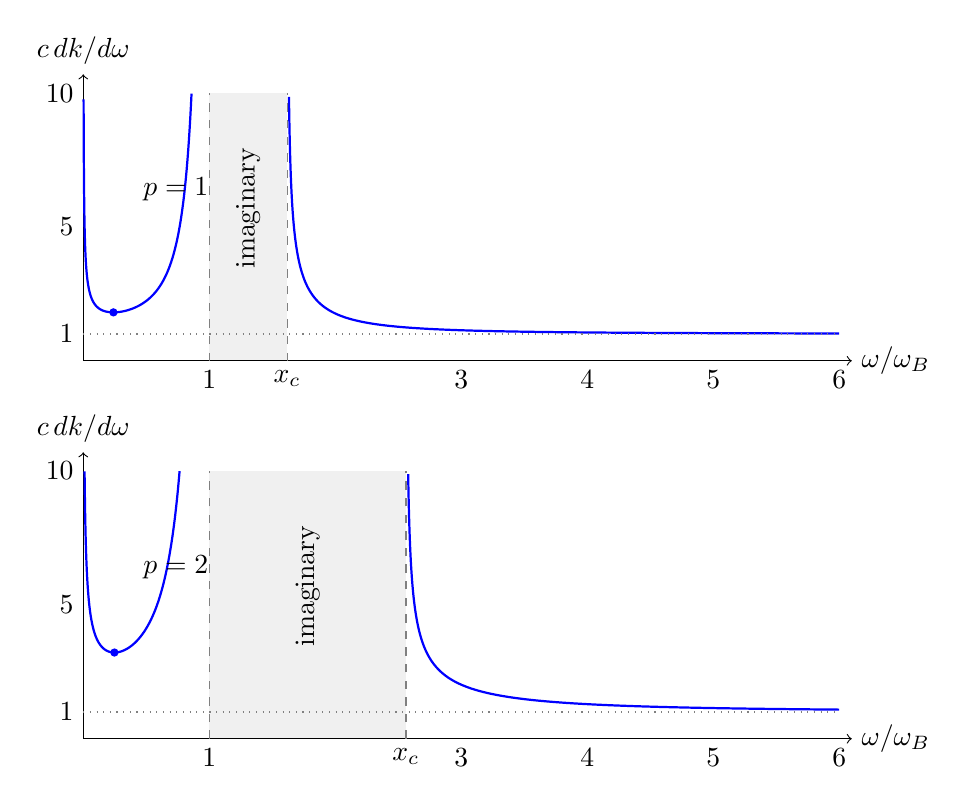
\begin{tikzpicture}[x=1.6cm,y=.34cm]
\begin{scope}[yshift=0.0cm]
\fill[gray!12] (1,0) rectangle (1.618033988749895,10);
\draw[->] (0,0)--(6.1,0) node[right] {$\omega/\omega_B$};\draw[->] (0,0)--(0,10.7) node[above] {$c\,dk/d\omega$};
\draw[blue,thick] plot coordinates {(0.002663,9.765927) (0.003218,8.899473) (0.003772,8.233009) (0.004327,7.700063) (0.004881,7.261465) (0.005436,6.892441) (0.005990,6.576456) (0.006544,6.301995) (0.007099,6.060762) (0.007653,5.846608) (0.008208,5.654865) (0.008762,5.481918) (0.009317,5.324918) (0.009871,5.181584) (0.010426,5.050068) (0.010980,4.928853) (0.011534,4.816680) (0.012089,4.712495) (0.012643,4.615409) (0.013198,4.524665) (0.013752,4.439613) (0.014307,4.359694) (0.014861,4.284422) (0.015416,4.213372) (0.015970,4.146173) (0.016524,4.082497) (0.017079,4.022054) (0.017633,3.964586) (0.018188,3.909863) (0.018742,3.857679) (0.019297,3.807849) (0.019851,3.760206) (0.020406,3.714600) (0.020960,3.670893) (0.021514,3.628963) (0.022069,3.588695) (0.022623,3.549986) (0.023178,3.512741) (0.023732,3.476874) (0.024287,3.442306) (0.024841,3.408961) (0.025396,3.376773) (0.025950,3.345679) (0.026504,3.315621) (0.027059,3.286545) (0.027613,3.258401) (0.028168,3.231141) (0.028722,3.204724) (0.029277,3.179108) (0.029831,3.154256) (0.030386,3.130132) (0.030940,3.106703) (0.031494,3.083938) (0.032049,3.061808) (0.032603,3.040285) (0.033158,3.019343) (0.033712,2.998959) (0.034267,2.979109) (0.034821,2.959772) (0.035376,2.940927) (0.035930,2.922554) (0.036484,2.904637) (0.037039,2.887157) (0.037593,2.870097) (0.038148,2.853443) (0.038702,2.837180) (0.039257,2.821293) (0.039811,2.805769) (0.040366,2.790596) (0.040920,2.775761) (0.041474,2.761253) (0.042029,2.747061) (0.042583,2.733175) (0.043138,2.719583) (0.043692,2.706278) (0.044247,2.693249) (0.044801,2.680489) (0.045356,2.667988) (0.045910,2.655738) (0.046464,2.643733) (0.047019,2.631964) (0.047573,2.620425) (0.048128,2.609109) (0.048682,2.598009) (0.049237,2.587120) (0.049791,2.576434) (0.050346,2.565947) (0.050900,2.555653) (0.051454,2.545547) (0.052009,2.535624) (0.052563,2.525878) (0.053118,2.516304) (0.053672,2.506900) (0.054227,2.497659) (0.054781,2.488578) (0.055336,2.479652) (0.055890,2.470878) (0.056444,2.462253) (0.056999,2.453771) (0.057553,2.445430) (0.058108,2.437226) (0.058662,2.429156) (0.059217,2.421217) (0.059771,2.413405) (0.060326,2.405718) (0.060880,2.398153) (0.061434,2.390706) (0.061989,2.383376) (0.062543,2.376159) (0.063098,2.369054) (0.063652,2.362056) (0.064207,2.355165) (0.064761,2.348378) (0.065316,2.341692) (0.065870,2.335106) (0.066424,2.328617) (0.066979,2.322223) (0.067533,2.315922) (0.068088,2.309713) (0.068642,2.303593) (0.069197,2.297560) (0.069751,2.291613) (0.070306,2.285750) (0.070860,2.279970) (0.071414,2.274270) (0.071969,2.268649) (0.072523,2.263106) (0.073078,2.257639) (0.073632,2.252246) (0.074187,2.246927) (0.074741,2.241679) (0.075296,2.236502) (0.075850,2.231394) (0.076404,2.226354) (0.076959,2.221380) (0.077513,2.216471) (0.078068,2.211627) (0.078622,2.206846) (0.079177,2.202127) (0.079731,2.197468) (0.080286,2.192869) (0.080840,2.188329) (0.081394,2.183846) (0.081949,2.179420) (0.082503,2.175050) (0.083058,2.170734) (0.083612,2.166472) (0.084167,2.162263) (0.084721,2.158106) (0.085276,2.154001) (0.085830,2.149945) (0.086384,2.145939) (0.086939,2.141981) (0.087493,2.138072) (0.088048,2.134209) (0.088602,2.130393) (0.089157,2.126622) (0.089711,2.122896) (0.090266,2.119215) (0.090820,2.115577) (0.091374,2.111981) (0.091929,2.108428) (0.092483,2.104916) (0.093038,2.101446) (0.093592,2.098015) (0.094147,2.094624) (0.094701,2.091272) (0.095256,2.087959) (0.095810,2.084683) (0.096364,2.081445) (0.096919,2.078244) (0.097473,2.075079) (0.098028,2.071950) (0.098582,2.068855) (0.099137,2.065796) (0.099691,2.062771) (0.100246,2.059780) (0.100800,2.056821) (0.101354,2.053896) (0.101909,2.051003) (0.102463,2.048142) (0.103018,2.045313) (0.103572,2.042514) (0.104127,2.039746) (0.104681,2.037009) (0.105236,2.034301) (0.105790,2.031623) (0.106344,2.028973) (0.106899,2.026353) (0.107453,2.023760) (0.108008,2.021195) (0.108562,2.018658) (0.109117,2.016149) (0.109671,2.013666) (0.110226,2.011209) (0.110780,2.008779) (0.111334,2.006374) (0.111889,2.003995) (0.112443,2.001641) (0.112998,1.999312) (0.113552,1.997008) (0.114107,1.994727) (0.114661,1.992471) (0.115216,1.990239) (0.115770,1.988029) (0.116324,1.985843) (0.116879,1.983680) (0.117433,1.981539) (0.117988,1.979421) (0.118542,1.977324) (0.119097,1.975250) (0.119651,1.973197) (0.120206,1.971165) (0.120760,1.969154) (0.121314,1.967164) (0.121869,1.965194) (0.122423,1.963245) (0.122978,1.961316) (0.123532,1.959406) (0.124087,1.957516) (0.124641,1.955646) (0.125196,1.953795) (0.125750,1.951963) (0.126304,1.950149) (0.126859,1.948354) (0.127413,1.946578) (0.127968,1.944820) (0.128522,1.943079) (0.129077,1.941356) (0.129631,1.939651) (0.130186,1.937964) (0.130740,1.936293) (0.131294,1.934640) (0.131849,1.933003) (0.132403,1.931383) (0.132958,1.929780) (0.133512,1.928193) (0.134067,1.926622) (0.134621,1.925067) (0.135176,1.923528) (0.135730,1.922004) (0.136284,1.920496) (0.136839,1.919004) (0.137393,1.917526) (0.137948,1.916064) (0.138502,1.914617) (0.139057,1.913184) (0.139611,1.911766) (0.140166,1.910362) (0.140720,1.908973) (0.141274,1.907598) (0.141829,1.906237) (0.142383,1.904890) (0.142938,1.903557) (0.143492,1.902237) (0.144047,1.900931) (0.144601,1.899638) (0.145156,1.898359) (0.145710,1.897093) (0.146264,1.895839) (0.146819,1.894599) (0.147373,1.893372) (0.147928,1.892157) (0.148482,1.890954) (0.149037,1.889765) (0.149591,1.888587) (0.150146,1.887422) (0.150700,1.886269) (0.151254,1.885127) (0.151809,1.883998) (0.152363,1.882881) (0.152918,1.881775) (0.153472,1.880681) (0.154027,1.879598) (0.154581,1.878527) (0.155136,1.877467) (0.155690,1.876418) (0.156244,1.875380) (0.156799,1.874353) (0.157353,1.873338) (0.157908,1.872333) (0.158462,1.871338) (0.159017,1.870355) (0.159571,1.869382) (0.160126,1.868419) (0.160680,1.867467) (0.161234,1.866525) (0.161789,1.865593) (0.162343,1.864672) (0.162898,1.863760) (0.163452,1.862859) (0.164007,1.861967) (0.164561,1.861085) (0.165116,1.860213) (0.165670,1.859351) (0.166224,1.858498) (0.166779,1.857655) (0.167333,1.856821) (0.167888,1.855996) (0.168442,1.855181) (0.168997,1.854375) (0.169551,1.853578) (0.170106,1.852790) (0.170660,1.852011) (0.171214,1.851242) (0.171769,1.850481) (0.172323,1.849728) (0.172878,1.848985) (0.173432,1.848250) (0.173987,1.847524) (0.174541,1.846807) (0.175096,1.846098) (0.175650,1.845397) (0.176204,1.844705) (0.176759,1.844021) (0.177313,1.843345) (0.177868,1.842678) (0.178422,1.842018) (0.178977,1.841367) (0.179531,1.840724) (0.180086,1.840088) (0.180640,1.839461) (0.181194,1.838841) (0.181749,1.838230) (0.182303,1.837626) (0.182858,1.837029) (0.183412,1.836441) (0.183967,1.835860) (0.184521,1.835286) (0.185076,1.834720) (0.185630,1.834162) (0.186184,1.833611) (0.186739,1.833067) (0.187293,1.832530) (0.187848,1.832001) (0.188402,1.831479) (0.188957,1.830964) (0.189511,1.830457) (0.190066,1.829956) (0.190620,1.829462) (0.191174,1.828976) (0.191729,1.828496) (0.192283,1.828023) (0.192838,1.827557) (0.193392,1.827098) (0.193947,1.826645) (0.194501,1.826200) (0.195056,1.825761) (0.195610,1.825329) (0.196164,1.824903) (0.196719,1.824484) (0.197273,1.824071) (0.197828,1.823665) (0.198382,1.823265) (0.198937,1.822872) (0.199491,1.822485) (0.200046,1.822104) (0.200600,1.821730) (0.201154,1.821362) (0.201709,1.821001) (0.202263,1.820645) (0.202818,1.820296) (0.203372,1.819952) (0.203927,1.819615) (0.204481,1.819284) (0.205036,1.818959) (0.205590,1.818640) (0.206144,1.818327) (0.206699,1.818020) (0.207253,1.817718) (0.207808,1.817423) (0.208362,1.817133) (0.208917,1.816850) (0.209471,1.816572) (0.210026,1.816299) (0.210580,1.816033) (0.211134,1.815772) (0.211689,1.815517) (0.212243,1.815267) (0.212798,1.815023) (0.213352,1.814785) (0.213907,1.814552) (0.214461,1.814325) (0.215016,1.814103) (0.215570,1.813886) (0.216124,1.813676) (0.216679,1.813470) (0.217233,1.813270) (0.217788,1.813075) (0.218342,1.812886) (0.218897,1.812701) (0.219451,1.812522) (0.220006,1.812349) (0.220560,1.812180) (0.221114,1.812017) (0.221669,1.811859) (0.222223,1.811706) (0.222778,1.811559) (0.223332,1.811416) (0.223887,1.811278) (0.224441,1.811146) (0.224996,1.811019) (0.225550,1.810896) (0.226104,1.810779) (0.226659,1.810666) (0.227213,1.810559) (0.227768,1.810457) (0.228322,1.810359) (0.228877,1.810266) (0.229431,1.810178) (0.229986,1.810095) (0.230540,1.810017) (0.231094,1.809944) (0.231649,1.809875) (0.232203,1.809812) (0.232758,1.809753) (0.233312,1.809698) (0.233867,1.809649) (0.234421,1.809604) (0.234976,1.809564) (0.235530,1.809528) (0.236084,1.809497) (0.236639,1.809471) (0.237193,1.809450) (0.237748,1.809433) (0.238302,1.809420) (0.238857,1.809412) (0.239411,1.809409) (0.239966,1.809410) (0.240520,1.809416) (0.241074,1.809426) (0.241629,1.809440) (0.242183,1.809459) (0.242738,1.809483) (0.243292,1.809511) (0.243847,1.809543) (0.244401,1.809580) (0.244956,1.809621) (0.245510,1.809667) (0.246064,1.809717) (0.246619,1.809771) (0.247173,1.809829) (0.247728,1.809892) (0.248282,1.809959) (0.248837,1.810031) (0.249391,1.810106) (0.249946,1.810186) (0.250500,1.810270) (0.251054,1.810359) (0.251609,1.810451) (0.252163,1.810548) (0.252718,1.810649) (0.253272,1.810754) (0.253827,1.810864) (0.254381,1.810977) (0.254936,1.811095) (0.255490,1.811216) (0.256044,1.811342) (0.256599,1.811472) (0.257153,1.811606) (0.257708,1.811744) (0.258262,1.811886) (0.258817,1.812033) (0.259371,1.812183) (0.259926,1.812337) (0.260480,1.812496) (0.261034,1.812658) (0.261589,1.812824) (0.262143,1.812995) (0.262698,1.813169) (0.263252,1.813347) (0.263807,1.813530) (0.264361,1.813716) (0.264916,1.813906) (0.265470,1.814100) (0.266024,1.814298) (0.266579,1.814500) (0.267133,1.814706) (0.267688,1.814915) (0.268242,1.815129) (0.268797,1.815346) (0.269351,1.815568) (0.269906,1.815793) (0.270460,1.816022) (0.271014,1.816255) (0.271569,1.816491) (0.272123,1.816732) (0.272678,1.816976) (0.273232,1.817224) (0.273787,1.817476) (0.274341,1.817732) (0.274896,1.817992) (0.275450,1.818255) (0.276004,1.818522) (0.276559,1.818793) (0.277113,1.819067) (0.277668,1.819346) (0.278222,1.819628) (0.278777,1.819913) (0.279331,1.820203) (0.279886,1.820496) (0.280440,1.820793) (0.280994,1.821094) (0.281549,1.821398) (0.282103,1.821706) (0.282658,1.822018) (0.283212,1.822333) (0.283767,1.822652) (0.284321,1.822975) (0.284876,1.823301) (0.285430,1.823631) (0.285984,1.823965) (0.286539,1.824303) (0.287093,1.824644) (0.287648,1.824988) (0.288202,1.825336) (0.288757,1.825688) (0.289311,1.826044) (0.289866,1.826403) (0.290420,1.826765) (0.290974,1.827132) (0.291529,1.827502) (0.292083,1.827875) (0.292638,1.828252) (0.293192,1.828633) (0.293747,1.829017) (0.294301,1.829405) (0.294856,1.829796) (0.295410,1.830191) (0.295964,1.830590) (0.296519,1.830992) (0.297073,1.831397) (0.297628,1.831807) (0.298182,1.832219) (0.298737,1.832635) (0.299291,1.833055) (0.299846,1.833479) (0.300400,1.833905) (0.300954,1.834336) (0.301509,1.834770) (0.302063,1.835207) (0.302618,1.835648) (0.303172,1.836092) (0.303727,1.836540) (0.304281,1.836992) (0.304836,1.837447) (0.305390,1.837905) (0.305944,1.838367) (0.306499,1.838833) (0.307053,1.839302) (0.307608,1.839774) (0.308162,1.840250) (0.308717,1.840730) (0.309271,1.841212) (0.309826,1.841699) (0.310380,1.842189) (0.310934,1.842682) (0.311489,1.843179) (0.312043,1.843679) (0.312598,1.844183) (0.313152,1.844690) (0.313707,1.845201) (0.314261,1.845715) (0.314816,1.846233) (0.315370,1.846754) (0.315924,1.847278) (0.316479,1.847807) (0.317033,1.848338) (0.317588,1.848873) (0.318142,1.849411) (0.318697,1.849953) (0.319251,1.850499) (0.319806,1.851047) (0.320360,1.851600) (0.320914,1.852155) (0.321469,1.852714) (0.322023,1.853277) (0.322578,1.853843) (0.323132,1.854413) (0.323687,1.854986) (0.324241,1.855562) (0.324796,1.856142) (0.325350,1.856725) (0.325904,1.857312) (0.326459,1.857902) (0.327013,1.858496) (0.327568,1.859093) (0.328122,1.859693) (0.328677,1.860297) (0.329231,1.860905) (0.329786,1.861516) (0.330340,1.862130) (0.330894,1.862748) (0.331449,1.863369) (0.332003,1.863994) (0.332558,1.864622) (0.333112,1.865253) (0.333667,1.865888) (0.334221,1.866527) (0.334776,1.867169) (0.335330,1.867814) (0.335884,1.868463) (0.336439,1.869116) (0.336993,1.869771) (0.337548,1.870431) (0.338102,1.871093) (0.338657,1.871759) (0.339211,1.872429) (0.339766,1.873102) (0.340320,1.873779) (0.340874,1.874459) (0.341429,1.875142) (0.341983,1.875829) (0.342538,1.876520) (0.343092,1.877213) (0.343647,1.877911) (0.344201,1.878612) (0.344756,1.879316) (0.345310,1.880024) (0.345864,1.880735) (0.346419,1.881450) (0.346973,1.882168) (0.347528,1.882890) (0.348082,1.883615) (0.348637,1.884344) (0.349191,1.885076) (0.349746,1.885812) (0.350300,1.886551) (0.350854,1.887294) (0.351409,1.888040) (0.351963,1.888790) (0.352518,1.889543) (0.353072,1.890300) (0.353627,1.891060) (0.354181,1.891824) (0.354736,1.892592) (0.355290,1.893362) (0.355844,1.894137) (0.356399,1.894915) (0.356953,1.895696) (0.357508,1.896481) (0.358062,1.897270) (0.358617,1.898062) (0.359171,1.898858) (0.359726,1.899657) (0.360280,1.900460) (0.360834,1.901266) (0.361389,1.902076) (0.361943,1.902889) (0.362498,1.903706) (0.363052,1.904527) (0.363607,1.905351) (0.364161,1.906179) (0.364716,1.907010) (0.365270,1.907845) (0.365824,1.908684) (0.366379,1.909526) (0.366933,1.910372) (0.367488,1.911221) (0.368042,1.912074) (0.368597,1.912930) (0.369151,1.913791) (0.369706,1.914654) (0.370260,1.915522) (0.370814,1.916393) (0.371369,1.917268) (0.371923,1.918146) (0.372478,1.919028) (0.373032,1.919914) (0.373587,1.920803) (0.374141,1.921696) (0.374696,1.922593) (0.375250,1.923493) (0.375804,1.924397) (0.376359,1.925305) (0.376913,1.926216) (0.377468,1.927131) (0.378022,1.928050) (0.378577,1.928972) (0.379131,1.929898) (0.379686,1.930828) (0.380240,1.931762) (0.380794,1.932699) (0.381349,1.933640) (0.381903,1.934585) (0.382458,1.935534) (0.383012,1.936486) (0.383567,1.937442) (0.384121,1.938402) (0.384676,1.939366) (0.385230,1.940333) (0.385784,1.941304) (0.386339,1.942279) (0.386893,1.943258) (0.387448,1.944240) (0.388002,1.945227) (0.388557,1.946217) (0.389111,1.947211) (0.389666,1.948208) (0.390220,1.949210) (0.390774,1.950216) (0.391329,1.951225) (0.391883,1.952238) (0.392438,1.953255) (0.392992,1.954276) (0.393547,1.955301) (0.394101,1.956329) (0.394656,1.957362) (0.395210,1.958398) (0.395764,1.959439) (0.396319,1.960483) (0.396873,1.961531) (0.397428,1.962583) (0.397982,1.963639) (0.398537,1.964699) (0.399091,1.965763) (0.399646,1.966831) (0.400200,1.967903) (0.400754,1.968978) (0.401309,1.970058) (0.401863,1.971142) (0.402418,1.972230) (0.402972,1.973321) (0.403527,1.974417) (0.404081,1.975517) (0.404636,1.976621) (0.405190,1.977728) (0.405744,1.978840) (0.406299,1.979956) (0.406853,1.981076) (0.407408,1.982200) (0.407962,1.983328) (0.408517,1.984460) (0.409071,1.985597) (0.409626,1.986737) (0.410180,1.987882) (0.410734,1.989030) (0.411289,1.990183) (0.411843,1.991340) (0.412398,1.992501) (0.412952,1.993666) (0.413507,1.994835) (0.414061,1.996009) (0.414616,1.997187) (0.415170,1.998369) (0.415724,1.999555) (0.416279,2.000745) (0.416833,2.001940) (0.417388,2.003138) (0.417942,2.004341) (0.418497,2.005549) (0.419051,2.006760) (0.419606,2.007976) (0.420160,2.009196) (0.420714,2.010420) (0.421269,2.011649) (0.421823,2.012882) (0.422378,2.014119) (0.422932,2.015361) (0.423487,2.016607) (0.424041,2.017857) (0.424596,2.019112) (0.425150,2.020371) (0.425704,2.021635) (0.426259,2.022903) (0.426813,2.024175) (0.427368,2.025452) (0.427922,2.026733) (0.428477,2.028018) (0.429031,2.029308) (0.429586,2.030603) (0.430140,2.031902) (0.430694,2.033205) (0.431249,2.034513) (0.431803,2.035825) (0.432358,2.037142) (0.432912,2.038464) (0.433467,2.039790) (0.434021,2.041120) (0.434576,2.042456) (0.435130,2.043795) (0.435684,2.045140) (0.436239,2.046488) (0.436793,2.047842) (0.437348,2.049200) (0.437902,2.050563) (0.438457,2.051930) (0.439011,2.053302) (0.439566,2.054679) (0.440120,2.056061) (0.440674,2.057447) (0.441229,2.058838) (0.441783,2.060233) (0.442338,2.061634) (0.442892,2.063039) (0.443447,2.064449) (0.444001,2.065863) (0.444556,2.067283) (0.445110,2.068707) (0.445664,2.070136) (0.446219,2.071570) (0.446773,2.073009) (0.447328,2.074452) (0.447882,2.075901) (0.448437,2.077354) (0.448991,2.078812) (0.449546,2.080275) (0.450100,2.081743) (0.450654,2.083217) (0.451209,2.084695) (0.451763,2.086177) (0.452318,2.087665) (0.452872,2.089158) (0.453427,2.090656) (0.453981,2.092159) (0.454536,2.093667) (0.455090,2.095180) (0.455644,2.096699) (0.456199,2.098222) (0.456753,2.099750) (0.457308,2.101284) (0.457862,2.102822) (0.458417,2.104366) (0.458971,2.105915) (0.459526,2.107469) (0.460080,2.109028) (0.460634,2.110593) (0.461189,2.112162) (0.461743,2.113737) (0.462298,2.115317) (0.462852,2.116903) (0.463407,2.118494) (0.463961,2.120090) (0.464516,2.121691) (0.465070,2.123298) (0.465624,2.124910) (0.466179,2.126527) (0.466733,2.128150) (0.467288,2.129779) (0.467842,2.131412) (0.468397,2.133051) (0.468951,2.134696) (0.469506,2.136346) (0.470060,2.138001) (0.470614,2.139662) (0.471169,2.141329) (0.471723,2.143001) (0.472278,2.144679) (0.472832,2.146362) (0.473387,2.148051) (0.473941,2.149745) (0.474496,2.151445) (0.475050,2.153151) (0.475604,2.154862) (0.476159,2.156579) (0.476713,2.158302) (0.477268,2.160031) (0.477822,2.161765) (0.478377,2.163505) (0.478931,2.165251) (0.479486,2.167002) (0.480040,2.168760) (0.480594,2.170523) (0.481149,2.172292) (0.481703,2.174067) (0.482258,2.175848) (0.482812,2.177634) (0.483367,2.179427) (0.483921,2.181226) (0.484476,2.183030) (0.485030,2.184841) (0.485584,2.186658) (0.486139,2.188480) (0.486693,2.190309) (0.487248,2.192144) (0.487802,2.193984) (0.488357,2.195831) (0.488911,2.197685) (0.489466,2.199544) (0.490020,2.201409) (0.490574,2.203281) (0.491129,2.205159) (0.491683,2.207043) (0.492238,2.208933) (0.492792,2.210830) (0.493347,2.212733) (0.493901,2.214642) (0.494456,2.216558) (0.495010,2.218480) (0.495564,2.220408) (0.496119,2.222343) (0.496673,2.224284) (0.497228,2.226232) (0.497782,2.228186) (0.498337,2.230147) (0.498891,2.232114) (0.499446,2.234088) (0.500000,2.236068) (0.500554,2.238055) (0.501109,2.240048) (0.501663,2.242049) (0.502218,2.244056) (0.502772,2.246069) (0.503327,2.248089) (0.503881,2.250116) (0.504436,2.252150) (0.504990,2.254191) (0.505544,2.256238) (0.506099,2.258293) (0.506653,2.260354) (0.507208,2.262422) (0.507762,2.264497) (0.508317,2.266578) (0.508871,2.268667) (0.509426,2.270763) (0.509980,2.272866) (0.510534,2.274976) (0.511089,2.277093) (0.511643,2.279217) (0.512198,2.281348) (0.512752,2.283486) (0.513307,2.285632) (0.513861,2.287784) (0.514416,2.289944) (0.514970,2.292111) (0.515524,2.294286) (0.516079,2.296468) (0.516633,2.298657) (0.517188,2.300853) (0.517742,2.303057) (0.518297,2.305268) (0.518851,2.307487) (0.519406,2.309713) (0.519960,2.311947) (0.520514,2.314188) (0.521069,2.316437) (0.521623,2.318693) (0.522178,2.320957) (0.522732,2.323229) (0.523287,2.325508) (0.523841,2.327795) (0.524396,2.330090) (0.524950,2.332392) (0.525504,2.334703) (0.526059,2.337021) (0.526613,2.339347) (0.527168,2.341681) (0.527722,2.344022) (0.528277,2.346372) (0.528831,2.348730) (0.529386,2.351096) (0.529940,2.353469) (0.530494,2.355851) (0.531049,2.358241) (0.531603,2.360639) (0.532158,2.363046) (0.532712,2.365460) (0.533267,2.367883) (0.533821,2.370314) (0.534376,2.372753) (0.534930,2.375201) (0.535484,2.377657) (0.536039,2.380121) (0.536593,2.382594) (0.537148,2.385075) (0.537702,2.387565) (0.538257,2.390063) (0.538811,2.392570) (0.539366,2.395085) (0.539920,2.397610) (0.540474,2.400142) (0.541029,2.402684) (0.541583,2.405234) (0.542138,2.407793) (0.542692,2.410361) (0.543247,2.412938) (0.543801,2.415523) (0.544356,2.418118) (0.544910,2.420721) (0.545464,2.423334) (0.546019,2.425955) (0.546573,2.428586) (0.547128,2.431226) (0.547682,2.433874) (0.548237,2.436532) (0.548791,2.439200) (0.549346,2.441876) (0.549900,2.444562) (0.550454,2.447257) (0.551009,2.449962) (0.551563,2.452676) (0.552118,2.455399) (0.552672,2.458132) (0.553227,2.460874) (0.553781,2.463626) (0.554336,2.466388) (0.554890,2.469159) (0.555444,2.471940) (0.555999,2.474731) (0.556553,2.477532) (0.557108,2.480342) (0.557662,2.483162) (0.558217,2.485992) (0.558771,2.488832) (0.559326,2.491682) (0.559880,2.494542) (0.560434,2.497413) (0.560989,2.500293) (0.561543,2.503183) (0.562098,2.506084) (0.562652,2.508995) (0.563207,2.511916) (0.563761,2.514848) (0.564316,2.517790) (0.564870,2.520742) (0.565424,2.523705) (0.565979,2.526678) (0.566533,2.529662) (0.567088,2.532657) (0.567642,2.535662) (0.568197,2.538678) (0.568751,2.541705) (0.569306,2.544742) (0.569860,2.547790) (0.570414,2.550850) (0.570969,2.553920) (0.571523,2.557001) (0.572078,2.560093) (0.572632,2.563197) (0.573187,2.566311) (0.573741,2.569437) (0.574296,2.572574) (0.574850,2.575722) (0.575404,2.578881) (0.575959,2.582052) (0.576513,2.585235) (0.577068,2.588428) (0.577622,2.591634) (0.578177,2.594851) (0.578731,2.598080) (0.579286,2.601320) (0.579840,2.604572) (0.580394,2.607836) (0.580949,2.611112) (0.581503,2.614400) (0.582058,2.617700) (0.582612,2.621011) (0.583167,2.624335) (0.583721,2.627671) (0.584276,2.631019) (0.584830,2.634380) (0.585384,2.637753) (0.585939,2.641138) (0.586493,2.644535) (0.587048,2.647945) (0.587602,2.651368) (0.588157,2.654803) (0.588711,2.658251) (0.589266,2.661711) (0.589820,2.665185) (0.590374,2.668671) (0.590929,2.672170) (0.591483,2.675682) (0.592038,2.679207) (0.592592,2.682745) (0.593147,2.686296) (0.593701,2.689861) (0.594256,2.693439) (0.594810,2.697030) (0.595364,2.700634) (0.595919,2.704252) (0.596473,2.707883) (0.597028,2.711528) (0.597582,2.715187) (0.598137,2.718859) (0.598691,2.722546) (0.599246,2.726246) (0.599800,2.729959) (0.600354,2.733687) (0.600909,2.737429) (0.601463,2.741185) (0.602018,2.744955) (0.602572,2.748740) (0.603127,2.752539) (0.603681,2.756352) (0.604236,2.760180) (0.604790,2.764022) (0.605344,2.767878) (0.605899,2.771750) (0.606453,2.775636) (0.607008,2.779537) (0.607562,2.783453) (0.608117,2.787384) (0.608671,2.791330) (0.609226,2.795291) (0.609780,2.799267) (0.610334,2.803258) (0.610889,2.807265) (0.611443,2.811287) (0.611998,2.815325) (0.612552,2.819378) (0.613107,2.823447) (0.613661,2.827532) (0.614216,2.831632) (0.614770,2.835748) (0.615324,2.839881) (0.615879,2.844029) (0.616433,2.848193) (0.616988,2.852374) (0.617542,2.856571) (0.618097,2.860784) (0.618651,2.865014) (0.619206,2.869260) (0.619760,2.873523) (0.620314,2.877803) (0.620869,2.882099) (0.621423,2.886412) (0.621978,2.890742) (0.622532,2.895090) (0.623087,2.899454) (0.623641,2.903835) (0.624196,2.908234) (0.624750,2.912651) (0.625304,2.917084) (0.625859,2.921536) (0.626413,2.926005) (0.626968,2.930492) (0.627522,2.934996) (0.628077,2.939519) (0.628631,2.944060) (0.629186,2.948618) (0.629740,2.953195) (0.630294,2.957791) (0.630849,2.962404) (0.631403,2.967037) (0.631958,2.971688) (0.632512,2.976357) (0.633067,2.981046) (0.633621,2.985753) (0.634176,2.990479) (0.634730,2.995225) (0.635284,2.999990) (0.635839,3.004774) (0.636393,3.009577) (0.636948,3.014400) (0.637502,3.019243) (0.638057,3.024105) (0.638611,3.028987) (0.639166,3.033889) (0.639720,3.038811) (0.640274,3.043754) (0.640829,3.048716) (0.641383,3.053699) (0.641938,3.058703) (0.642492,3.063727) (0.643047,3.068772) (0.643601,3.073837) (0.644156,3.078924) (0.644710,3.084032) (0.645264,3.089160) (0.645819,3.094311) (0.646373,3.099482) (0.646928,3.104675) (0.647482,3.109890) (0.648037,3.115126) (0.648591,3.120385) (0.649146,3.125665) (0.649700,3.130967) (0.650254,3.136292) (0.650809,3.141639) (0.651363,3.147009) (0.651918,3.152401) (0.652472,3.157816) (0.653027,3.163254) (0.653581,3.168715) (0.654136,3.174199) (0.654690,3.179706) (0.655244,3.185237) (0.655799,3.190791) (0.656353,3.196369) (0.656908,3.201970) (0.657462,3.207596) (0.658017,3.213246) (0.658571,3.218919) (0.659126,3.224618) (0.659680,3.230340) (0.660234,3.236088) (0.660789,3.241860) (0.661343,3.247657) (0.661898,3.253479) (0.662452,3.259326) (0.663007,3.265199) (0.663561,3.271097) (0.664116,3.277020) (0.664670,3.282970) (0.665224,3.288945) (0.665779,3.294947) (0.666333,3.300975) (0.666888,3.307029) (0.667442,3.313109) (0.667997,3.319217) (0.668551,3.325351) (0.669106,3.331512) (0.669660,3.337701) (0.670214,3.343916) (0.670769,3.350160) (0.671323,3.356431) (0.671878,3.362729) (0.672432,3.369056) (0.672987,3.375411) (0.673541,3.381794) (0.674096,3.388206) (0.674650,3.394647) (0.675204,3.401116) (0.675759,3.407614) (0.676313,3.414141) (0.676868,3.420698) (0.677422,3.427285) (0.677977,3.433901) (0.678531,3.440547) (0.679086,3.447223) (0.679640,3.453929) (0.680194,3.460666) (0.680749,3.467433) (0.681303,3.474231) (0.681858,3.481061) (0.682412,3.487921) (0.682967,3.494813) (0.683521,3.501736) (0.684076,3.508692) (0.684630,3.515679) (0.685184,3.522698) (0.685739,3.529750) (0.686293,3.536834) (0.686848,3.543951) (0.687402,3.551101) (0.687957,3.558285) (0.688511,3.565501) (0.689066,3.572752) (0.689620,3.580036) (0.690174,3.587354) (0.690729,3.594706) (0.691283,3.602093) (0.691838,3.609514) (0.692392,3.616971) (0.692947,3.624462) (0.693501,3.631989) (0.694056,3.639552) (0.694610,3.647150) (0.695164,3.654784) (0.695719,3.662455) (0.696273,3.670162) (0.696828,3.677906) (0.697382,3.685687) (0.697937,3.693504) (0.698491,3.701360) (0.699046,3.709253) (0.699600,3.717184) (0.700154,3.725153) (0.700709,3.733161) (0.701263,3.741207) (0.701818,3.749292) (0.702372,3.757417) (0.702927,3.765581) (0.703481,3.773784) (0.704036,3.782028) (0.704590,3.790312) (0.705144,3.798636) (0.705699,3.807001) (0.706253,3.815407) (0.706808,3.823854) (0.707362,3.832343) (0.707917,3.840874) (0.708471,3.849447) (0.709026,3.858063) (0.709580,3.866721) (0.710134,3.875422) (0.710689,3.884166) (0.711243,3.892954) (0.711798,3.901786) (0.712352,3.910662) (0.712907,3.919583) (0.713461,3.928548) (0.714016,3.937558) (0.714570,3.946614) (0.715124,3.955716) (0.715679,3.964863) (0.716233,3.974057) (0.716788,3.983297) (0.717342,3.992585) (0.717897,4.001920) (0.718451,4.011302) (0.719006,4.020732) (0.719560,4.030211) (0.720114,4.039738) (0.720669,4.049315) (0.721223,4.058940) (0.721778,4.068615) (0.722332,4.078341) (0.722887,4.088116) (0.723441,4.097942) (0.723996,4.107820) (0.724550,4.117749) (0.725104,4.127729) (0.725659,4.137762) (0.726213,4.147847) (0.726768,4.157986) (0.727322,4.168177) (0.727877,4.178422) (0.728431,4.188722) (0.728986,4.199076) (0.729540,4.209484) (0.730094,4.219948) (0.730649,4.230468) (0.731203,4.241043) (0.731758,4.251675) (0.732312,4.262364) (0.732867,4.273110) (0.733421,4.283914) (0.733976,4.294776) (0.734530,4.305697) (0.735084,4.316676) (0.735639,4.327715) (0.736193,4.338814) (0.736748,4.349973) (0.737302,4.361193) (0.737857,4.372474) (0.738411,4.383817) (0.738966,4.395222) (0.739520,4.406690) (0.740074,4.418220) (0.740629,4.429814) (0.741183,4.441472) (0.741738,4.453195) (0.742292,4.464983) (0.742847,4.476836) (0.743401,4.488755) (0.743956,4.500740) (0.744510,4.512793) (0.745064,4.524913) (0.745619,4.537101) (0.746173,4.549358) (0.746728,4.561683) (0.747282,4.574079) (0.747837,4.586544) (0.748391,4.599080) (0.748946,4.611688) (0.749500,4.624367) (0.750054,4.637119) (0.750609,4.649943) (0.751163,4.662841) (0.751718,4.675813) (0.752272,4.688860) (0.752827,4.701982) (0.753381,4.715180) (0.753936,4.728454) (0.754490,4.741805) (0.755044,4.755234) (0.755599,4.768742) (0.756153,4.782328) (0.756708,4.795994) (0.757262,4.809739) (0.757817,4.823566) (0.758371,4.837475) (0.758926,4.851465) (0.759480,4.865538) (0.760034,4.879695) (0.760589,4.893936) (0.761143,4.908261) (0.761698,4.922673) (0.762252,4.937170) (0.762807,4.951755) (0.763361,4.966427) (0.763916,4.981188) (0.764470,4.996037) (0.765024,5.010977) (0.765579,5.026007) (0.766133,5.041129) (0.766688,5.056343) (0.767242,5.071649) (0.767797,5.087050) (0.768351,5.102545) (0.768906,5.118135) (0.769460,5.133821) (0.770014,5.149604) (0.770569,5.165485) (0.771123,5.181465) (0.771678,5.197544) (0.772232,5.213723) (0.772787,5.230003) (0.773341,5.246386) (0.773896,5.262871) (0.774450,5.279460) (0.775004,5.296153) (0.775559,5.312953) (0.776113,5.329858) (0.776668,5.346871) (0.777222,5.363993) (0.777777,5.381224) (0.778331,5.398565) (0.778886,5.416017) (0.779440,5.433582) (0.779994,5.451260) (0.780549,5.469052) (0.781103,5.486959) (0.781658,5.504983) (0.782212,5.523124) (0.782767,5.541383) (0.783321,5.559762) (0.783876,5.578261) (0.784430,5.596882) (0.784984,5.615626) (0.785539,5.634494) (0.786093,5.653486) (0.786648,5.672605) (0.787202,5.691851) (0.787757,5.711225) (0.788311,5.730729) (0.788866,5.750364) (0.789420,5.770131) (0.789974,5.790031) (0.790529,5.810066) (0.791083,5.830236) (0.791638,5.850544) (0.792192,5.870989) (0.792747,5.891575) (0.793301,5.912301) (0.793856,5.933170) (0.794410,5.954182) (0.794964,5.975339) (0.795519,5.996642) (0.796073,6.018094) (0.796628,6.039694) (0.797182,6.061445) (0.797737,6.083349) (0.798291,6.105405) (0.798846,6.127617) (0.799400,6.149986) (0.799954,6.172512) (0.800509,6.195198) (0.801063,6.218045) (0.801618,6.241055) (0.802172,6.264230) (0.802727,6.287570) (0.803281,6.311078) (0.803836,6.334755) (0.804390,6.358603) (0.804944,6.382624) (0.805499,6.406820) (0.806053,6.431191) (0.806608,6.455741) (0.807162,6.480470) (0.807717,6.505381) (0.808271,6.530476) (0.808826,6.555755) (0.809380,6.581222) (0.809934,6.606878) (0.810489,6.632725) (0.811043,6.658765) (0.811598,6.685000) (0.812152,6.711433) (0.812707,6.738064) (0.813261,6.764897) (0.813816,6.791932) (0.814370,6.819174) (0.814924,6.846622) (0.815479,6.874281) (0.816033,6.902152) (0.816588,6.930237) (0.817142,6.958538) (0.817697,6.987058) (0.818251,7.015800) (0.818806,7.044765) (0.819360,7.073956) (0.819914,7.103376) (0.820469,7.133026) (0.821023,7.162910) (0.821578,7.193030) (0.822132,7.223389) (0.822687,7.253989) (0.823241,7.284832) (0.823796,7.315923) (0.824350,7.347262) (0.824904,7.378854) (0.825459,7.410700) (0.826013,7.442805) (0.826568,7.475170) (0.827122,7.507798) (0.827677,7.540693) (0.828231,7.573858) (0.828786,7.607295) (0.829340,7.641008) (0.829894,7.675000) (0.830449,7.709274) (0.831003,7.743834) (0.831558,7.778682) (0.832112,7.813822) (0.832667,7.849258) (0.833221,7.884993) (0.833776,7.921030) (0.834330,7.957373) (0.834884,7.994025) (0.835439,8.030991) (0.835993,8.068274) (0.836548,8.105877) (0.837102,8.143805) (0.837657,8.182062) (0.838211,8.220651) (0.838766,8.259576) (0.839320,8.298842) (0.839874,8.338453) (0.840429,8.378412) (0.840983,8.418725) (0.841538,8.459395) (0.842092,8.500427) (0.842647,8.541825) (0.843201,8.583594) (0.843756,8.625739) (0.844310,8.668264) (0.844864,8.711174) (0.845419,8.754474) (0.845973,8.798169) (0.846528,8.842264) (0.847082,8.886763) (0.847637,8.931673) (0.848191,8.976998) (0.848746,9.022743) (0.849300,9.068915) (0.849854,9.115518) (0.850409,9.162559) (0.850963,9.210043) (0.851518,9.257975) (0.852072,9.306363) (0.852627,9.355211) (0.853181,9.404526) (0.853736,9.454313) (0.854290,9.504581) (0.854844,9.555334) (0.855399,9.606579) (0.855953,9.658324) (0.856508,9.710574) (0.857062,9.763337) (0.857617,9.816619) (0.858171,9.870429) (0.858726,9.924772) (0.859280,9.979657)};
\draw[blue,thick] plot coordinates {(1.632740,9.859928) (1.635175,9.116173) (1.637609,8.515057) (1.640043,8.016014) (1.642478,7.593002) (1.644912,7.228431) (1.647346,6.909939) (1.649781,6.628543) (1.652215,6.377540) (1.654650,6.151814) (1.657084,5.947379) (1.659518,5.761081) (1.661953,5.590384) (1.664387,5.433224) (1.666821,5.287903) (1.669256,5.153005) (1.671690,5.027343) (1.674124,4.909911) (1.676559,4.799851) (1.678993,4.696426) (1.681428,4.598998) (1.683862,4.507013) (1.686296,4.419984) (1.688731,4.337486) (1.691165,4.259142) (1.693599,4.184619) (1.696034,4.113618) (1.698468,4.045875) (1.700903,3.981150) (1.703337,3.919229) (1.705771,3.859919) (1.708206,3.803044) (1.710640,3.748445) (1.713074,3.695977) (1.715509,3.645508) (1.717943,3.596916) (1.720378,3.550091) (1.722812,3.504931) (1.725246,3.461341) (1.727681,3.419236) (1.730115,3.378535) (1.732549,3.339164) (1.734984,3.301055) (1.737418,3.264143) (1.739852,3.228370) (1.742287,3.193680) (1.744721,3.160021) (1.747156,3.127345) (1.749590,3.095607) (1.752024,3.064765) (1.754459,3.034778) (1.756893,3.005611) (1.759327,2.977228) (1.761762,2.949595) (1.764196,2.922683) (1.766631,2.896461) (1.769065,2.870902) (1.771499,2.845980) (1.773934,2.821670) (1.776368,2.797950) (1.778802,2.774796) (1.781237,2.752188) (1.783671,2.730105) (1.786106,2.708530) (1.788540,2.687443) (1.790974,2.666829) (1.793409,2.646670) (1.795843,2.626951) (1.798277,2.607657) (1.800712,2.588775) (1.803146,2.570290) (1.805580,2.552191) (1.808015,2.534463) (1.810449,2.517097) (1.812884,2.500081) (1.815318,2.483403) (1.817752,2.467054) (1.820187,2.451024) (1.822621,2.435303) (1.825055,2.419882) (1.827490,2.404752) (1.829924,2.389906) (1.832359,2.375335) (1.834793,2.361031) (1.837227,2.346988) (1.839662,2.333197) (1.842096,2.319652) (1.844530,2.306346) (1.846965,2.293273) (1.849399,2.280427) (1.851834,2.267802) (1.854268,2.255392) (1.856702,2.243192) (1.859137,2.231196) (1.861571,2.219400) (1.864005,2.207797) (1.866440,2.196384) (1.868874,2.185156) (1.871308,2.174108) (1.873743,2.163237) (1.876177,2.152537) (1.878612,2.142005) (1.881046,2.131637) (1.883480,2.121429) (1.885915,2.111377) (1.888349,2.101479) (1.890783,2.091730) (1.893218,2.082126) (1.895652,2.072666) (1.898087,2.063346) (1.900521,2.054162) (1.902955,2.045111) (1.905390,2.036192) (1.907824,2.027400) (1.910258,2.018734) (1.912693,2.010191) (1.915127,2.001767) (1.917561,1.993462) (1.919996,1.985271) (1.922430,1.977194) (1.924865,1.969227) (1.927299,1.961368) (1.929733,1.953615) (1.932168,1.945967) (1.934602,1.938421) (1.937036,1.930975) (1.939471,1.923627) (1.941905,1.916375) (1.944340,1.909217) (1.946774,1.902152) (1.949208,1.895179) (1.951643,1.888294) (1.954077,1.881496) (1.956511,1.874785) (1.958946,1.868158) (1.961380,1.861614) (1.963815,1.855150) (1.966249,1.848767) (1.968683,1.842462) (1.971118,1.836234) (1.973552,1.830082) (1.975986,1.824004) (1.978421,1.817999) (1.980855,1.812066) (1.983289,1.806203) (1.985724,1.800409) (1.988158,1.794684) (1.990593,1.789025) (1.993027,1.783432) (1.995461,1.777904) (1.997896,1.772440) (2.000330,1.767038) (2.002764,1.761698) (2.005199,1.756418) (2.007633,1.751198) (2.010068,1.746036) (2.012502,1.740932) (2.014936,1.735885) (2.017371,1.730893) (2.019805,1.725957) (2.022239,1.721074) (2.024674,1.716245) (2.027108,1.711468) (2.029543,1.706743) (2.031977,1.702068) (2.034411,1.697444) (2.036846,1.692869) (2.039280,1.688342) (2.041714,1.683863) (2.044149,1.679430) (2.046583,1.675045) (2.049017,1.670705) (2.051452,1.666409) (2.053886,1.662159) (2.056321,1.657951) (2.058755,1.653787) (2.061189,1.649665) (2.063624,1.645585) (2.066058,1.641546) (2.068492,1.637548) (2.070927,1.633590) (2.073361,1.629671) (2.075796,1.625791) (2.078230,1.621949) (2.080664,1.618145) (2.083099,1.614378) (2.085533,1.610648) (2.087967,1.606955) (2.090402,1.603297) (2.092836,1.599674) (2.095271,1.596086) (2.097705,1.592532) (2.100139,1.589013) (2.102574,1.585526) (2.105008,1.582073) (2.107442,1.578652) (2.109877,1.575263) (2.112311,1.571905) (2.114745,1.568579) (2.117180,1.565284) (2.119614,1.562019) (2.122049,1.558784) (2.124483,1.555579) (2.126917,1.552403) (2.129352,1.549256) (2.131786,1.546137) (2.134220,1.543046) (2.136655,1.539984) (2.139089,1.536948) (2.141524,1.533940) (2.143958,1.530959) (2.146392,1.528003) (2.148827,1.525074) (2.151261,1.522171) (2.153695,1.519293) (2.156130,1.516441) (2.158564,1.513613) (2.160999,1.510809) (2.163433,1.508030) (2.165867,1.505275) (2.168302,1.502543) (2.170736,1.499835) (2.173170,1.497150) (2.175605,1.494487) (2.178039,1.491848) (2.180473,1.489230) (2.182908,1.486634) (2.185342,1.484061) (2.187777,1.481508) (2.190211,1.478977) (2.192645,1.476467) (2.195080,1.473977) (2.197514,1.471508) (2.199948,1.469060) (2.202383,1.466631) (2.204817,1.464222) (2.207252,1.461833) (2.209686,1.459463) (2.212120,1.457112) (2.214555,1.454781) (2.216989,1.452468) (2.219423,1.450173) (2.221858,1.447897) (2.224292,1.445638) (2.226726,1.443398) (2.229161,1.441176) (2.231595,1.438970) (2.234030,1.436783) (2.236464,1.434612) (2.238898,1.432458) (2.241333,1.430321) (2.243767,1.428201) (2.246201,1.426097) (2.248636,1.424009) (2.251070,1.421937) (2.253505,1.419881) (2.255939,1.417841) (2.258373,1.415816) (2.260808,1.413807) (2.263242,1.411813) (2.265676,1.409834) (2.268111,1.407870) (2.270545,1.405920) (2.272980,1.403985) (2.275414,1.402065) (2.277848,1.400159) (2.280283,1.398267) (2.282717,1.396389) (2.285151,1.394525) (2.287586,1.392674) (2.290020,1.390837) (2.292454,1.389014) (2.294889,1.387204) (2.297323,1.385407) (2.299758,1.383623) (2.302192,1.381852) (2.304626,1.380093) (2.307061,1.378348) (2.309495,1.376614) (2.311929,1.374894) (2.314364,1.373185) (2.316798,1.371489) (2.319233,1.369804) (2.321667,1.368132) (2.324101,1.366471) (2.326536,1.364822) (2.328970,1.363185) (2.331404,1.361559) (2.333839,1.359944) (2.336273,1.358341) (2.338708,1.356749) (2.341142,1.355168) (2.343576,1.353597) (2.346011,1.352038) (2.348445,1.350489) (2.350879,1.348951) (2.353314,1.347423) (2.355748,1.345906) (2.358182,1.344399) (2.360617,1.342902) (2.363051,1.341415) (2.365486,1.339939) (2.367920,1.338472) (2.370354,1.337015) (2.372789,1.335568) (2.375223,1.334131) (2.377657,1.332703) (2.380092,1.331284) (2.382526,1.329875) (2.384961,1.328475) (2.387395,1.327085) (2.389829,1.325704) (2.392264,1.324331) (2.394698,1.322968) (2.397132,1.321614) (2.399567,1.320268) (2.402001,1.318931) (2.404436,1.317603) (2.406870,1.316283) (2.409304,1.314972) (2.411739,1.313669) (2.414173,1.312375) (2.416607,1.311089) (2.419042,1.309811) (2.421476,1.308541) (2.423910,1.307280) (2.426345,1.306026) (2.428779,1.304780) (2.431214,1.303542) (2.433648,1.302312) (2.436082,1.301090) (2.438517,1.299875) (2.440951,1.298668) (2.443385,1.297469) (2.445820,1.296276) (2.448254,1.295092) (2.450689,1.293914) (2.453123,1.292744) (2.455557,1.291581) (2.457992,1.290425) (2.460426,1.289277) (2.462860,1.288135) (2.465295,1.287000) (2.467729,1.285872) (2.470163,1.284752) (2.472598,1.283637) (2.475032,1.282530) (2.477467,1.281429) (2.479901,1.280335) (2.482335,1.279248) (2.484770,1.278167) (2.487204,1.277092) (2.489638,1.276024) (2.492073,1.274962) (2.494507,1.273907) (2.496942,1.272858) (2.499376,1.271815) (2.501810,1.270778) (2.504245,1.269747) (2.506679,1.268722) (2.509113,1.267704) (2.511548,1.266691) (2.513982,1.265684) (2.516417,1.264683) (2.518851,1.263688) (2.521285,1.262699) (2.523720,1.261715) (2.526154,1.260738) (2.528588,1.259765) (2.531023,1.258799) (2.533457,1.257837) (2.535891,1.256882) (2.538326,1.255932) (2.540760,1.254987) (2.543195,1.254048) (2.545629,1.253114) (2.548063,1.252185) (2.550498,1.251261) (2.552932,1.250343) (2.555366,1.249430) (2.557801,1.248522) (2.560235,1.247619) (2.562670,1.246721) (2.565104,1.245829) (2.567538,1.244941) (2.569973,1.244058) (2.572407,1.243180) (2.574841,1.242307) (2.577276,1.241438) (2.579710,1.240575) (2.582145,1.239716) (2.584579,1.238862) (2.587013,1.238013) (2.589448,1.237168) (2.591882,1.236328) (2.594316,1.235493) (2.596751,1.234662) (2.599185,1.233835) (2.601619,1.233013) (2.604054,1.232196) (2.606488,1.231383) (2.608923,1.230574) (2.611357,1.229770) (2.613791,1.228970) (2.616226,1.228174) (2.618660,1.227382) (2.621094,1.226595) (2.623529,1.225812) (2.625963,1.225033) (2.628398,1.224258) (2.630832,1.223487) (2.633266,1.222721) (2.635701,1.221958) (2.638135,1.221200) (2.640569,1.220445) (2.643004,1.219694) (2.645438,1.218948) (2.647873,1.218205) (2.650307,1.217466) (2.652741,1.216731) (2.655176,1.216000) (2.657610,1.215272) (2.660044,1.214548) (2.662479,1.213828) (2.664913,1.213112) (2.667347,1.212400) (2.669782,1.211691) (2.672216,1.210985) (2.674651,1.210284) (2.677085,1.209586) (2.679519,1.208891) (2.681954,1.208200) (2.684388,1.207513) (2.686822,1.206829) (2.689257,1.206148) (2.691691,1.205471) (2.694126,1.204797) (2.696560,1.204127) (2.698994,1.203460) (2.701429,1.202796) (2.703863,1.202136) (2.706297,1.201479) (2.708732,1.200825) (2.711166,1.200175) (2.713600,1.199528) (2.716035,1.198884) (2.718469,1.198243) (2.720904,1.197605) (2.723338,1.196971) (2.725772,1.196339) (2.728207,1.195711) (2.730641,1.195086) (2.733075,1.194464) (2.735510,1.193845) (2.737944,1.193229) (2.740379,1.192616) (2.742813,1.192005) (2.745247,1.191398) (2.747682,1.190794) (2.750116,1.190193) (2.752550,1.189595) (2.754985,1.188999) (2.757419,1.188406) (2.759854,1.187817) (2.762288,1.187230) (2.764722,1.186646) (2.767157,1.186064) (2.769591,1.185486) (2.772025,1.184910) (2.774460,1.184337) (2.776894,1.183767) (2.779328,1.183199) (2.781763,1.182634) (2.784197,1.182072) (2.786632,1.181512) (2.789066,1.180955) (2.791500,1.180401) (2.793935,1.179849) (2.796369,1.179300) (2.798803,1.178753) (2.801238,1.178209) (2.803672,1.177668) (2.806107,1.177129) (2.808541,1.176592) (2.810975,1.176058) (2.813410,1.175527) (2.815844,1.174997) (2.818278,1.174471) (2.820713,1.173947) (2.823147,1.173425) (2.825582,1.172905) (2.828016,1.172388) (2.830450,1.171874) (2.832885,1.171361) (2.835319,1.170851) (2.837753,1.170344) (2.840188,1.169838) (2.842622,1.169335) (2.845056,1.168834) (2.847491,1.168336) (2.849925,1.167840) (2.852360,1.167346) (2.854794,1.166854) (2.857228,1.166364) (2.859663,1.165877) (2.862097,1.165392) (2.864531,1.164909) (2.866966,1.164428) (2.869400,1.163949) (2.871835,1.163472) (2.874269,1.162998) (2.876703,1.162525) (2.879138,1.162055) (2.881572,1.161587) (2.884006,1.161121) (2.886441,1.160657) (2.888875,1.160195) (2.891310,1.159735) (2.893744,1.159277) (2.896178,1.158821) (2.898613,1.158367) (2.901047,1.157915) (2.903481,1.157465) (2.905916,1.157017) (2.908350,1.156570) (2.910784,1.156126) (2.913219,1.155684) (2.915653,1.155244) (2.918088,1.154805) (2.920522,1.154369) (2.922956,1.153934) (2.925391,1.153501) (2.927825,1.153070) (2.930259,1.152641) (2.932694,1.152214) (2.935128,1.151788) (2.937563,1.151365) (2.939997,1.150943) (2.942431,1.150523) (2.944866,1.150105) (2.947300,1.149688) (2.949734,1.149274) (2.952169,1.148861) (2.954603,1.148449) (2.957037,1.148040) (2.959472,1.147632) (2.961906,1.147226) (2.964341,1.146822) (2.966775,1.146419) (2.969209,1.146018) (2.971644,1.145619) (2.974078,1.145221) (2.976512,1.144825) (2.978947,1.144431) (2.981381,1.144039) (2.983816,1.143648) (2.986250,1.143258) (2.988684,1.142870) (2.991119,1.142484) (2.993553,1.142100) (2.995987,1.141717) (2.998422,1.141335) (3.000856,1.140955) (3.003291,1.140577) (3.005725,1.140200) (3.008159,1.139825) (3.010594,1.139451) (3.013028,1.139079) (3.015462,1.138708) (3.017897,1.138339) (3.020331,1.137972) (3.022765,1.137606) (3.025200,1.137241) (3.027634,1.136878) (3.030069,1.136516) (3.032503,1.136156) (3.034937,1.135797) (3.037372,1.135439) (3.039806,1.135083) (3.042240,1.134729) (3.044675,1.134376) (3.047109,1.134024) (3.049544,1.133674) (3.051978,1.133325) (3.054412,1.132977) (3.056847,1.132631) (3.059281,1.132287) (3.061715,1.131943) (3.064150,1.131601) (3.066584,1.131261) (3.069019,1.130921) (3.071453,1.130583) (3.073887,1.130247) (3.076322,1.129911) (3.078756,1.129577) (3.081190,1.129245) (3.083625,1.128913) (3.086059,1.128583) (3.088493,1.128254) (3.090928,1.127927) (3.093362,1.127600) (3.095797,1.127275) (3.098231,1.126952) (3.100665,1.126629) (3.103100,1.126308) (3.105534,1.125988) (3.107968,1.125669) (3.110403,1.125352) (3.112837,1.125035) (3.115272,1.124720) (3.117706,1.124406) (3.120140,1.124094) (3.122575,1.123782) (3.125009,1.123472) (3.127443,1.123163) (3.129878,1.122855) (3.132312,1.122548) (3.134747,1.122243) (3.137181,1.121938) (3.139615,1.121635) (3.142050,1.121333) (3.144484,1.121032) (3.146918,1.120732) (3.149353,1.120433) (3.151787,1.120136) (3.154221,1.119839) (3.156656,1.119544) (3.159090,1.119250) (3.161525,1.118956) (3.163959,1.118664) (3.166393,1.118373) (3.168828,1.118084) (3.171262,1.117795) (3.173696,1.117507) (3.176131,1.117220) (3.178565,1.116935) (3.181000,1.116650) (3.183434,1.116367) (3.185868,1.116085) (3.188303,1.115803) (3.190737,1.115523) (3.193171,1.115244) (3.195606,1.114965) (3.198040,1.114688) (3.200474,1.114412) (3.202909,1.114137) (3.205343,1.113862) (3.207778,1.113589) (3.210212,1.113317) (3.212646,1.113046) (3.215081,1.112776) (3.217515,1.112506) (3.219949,1.112238) (3.222384,1.111971) (3.224818,1.111704) (3.227253,1.111439) (3.229687,1.111175) (3.232121,1.110911) (3.234556,1.110649) (3.236990,1.110387) (3.239424,1.110127) (3.241859,1.109867) (3.244293,1.109608) (3.246728,1.109350) (3.249162,1.109094) (3.251596,1.108838) (3.254031,1.108582) (3.256465,1.108328) (3.258899,1.108075) (3.261334,1.107823) (3.263768,1.107571) (3.266202,1.107321) (3.268637,1.107071) (3.271071,1.106822) (3.273506,1.106574) (3.275940,1.106327) (3.278374,1.106081) (3.280809,1.105836) (3.283243,1.105591) (3.285677,1.105348) (3.288112,1.105105) (3.290546,1.104863) (3.292981,1.104622) (3.295415,1.104382) (3.297849,1.104143) (3.300284,1.103904) (3.302718,1.103667) (3.305152,1.103430) (3.307587,1.103194) (3.310021,1.102959) (3.312456,1.102724) (3.314890,1.102491) (3.317324,1.102258) (3.319759,1.102026) (3.322193,1.101795) (3.324627,1.101564) (3.327062,1.101335) (3.329496,1.101106) (3.331930,1.100878) (3.334365,1.100651) (3.336799,1.100424) (3.339234,1.100199) (3.341668,1.099974) (3.344102,1.099750) (3.346537,1.099526) (3.348971,1.099304) (3.351405,1.099082) (3.353840,1.098861) (3.356274,1.098640) (3.358709,1.098421) (3.361143,1.098202) (3.363577,1.097984) (3.366012,1.097766) (3.368446,1.097550) (3.370880,1.097334) (3.373315,1.097119) (3.375749,1.096904) (3.378184,1.096690) (3.380618,1.096477) (3.383052,1.096265) (3.385487,1.096054) (3.387921,1.095843) (3.390355,1.095632) (3.392790,1.095423) (3.395224,1.095214) (3.397658,1.095006) (3.400093,1.094799) (3.402527,1.094592) (3.404962,1.094386) (3.407396,1.094181) (3.409830,1.093976) (3.412265,1.093772) (3.414699,1.093569) (3.417133,1.093366) (3.419568,1.093164) (3.422002,1.092963) (3.424437,1.092762) (3.426871,1.092562) (3.429305,1.092362) (3.431740,1.092164) (3.434174,1.091966) (3.436608,1.091768) (3.439043,1.091572) (3.441477,1.091375) (3.443911,1.091180) (3.446346,1.090985) (3.448780,1.090791) (3.451215,1.090597) (3.453649,1.090404) (3.456083,1.090212) (3.458518,1.090020) (3.460952,1.089829) (3.463386,1.089639) (3.465821,1.089449) (3.468255,1.089260) (3.470690,1.089071) (3.473124,1.088883) (3.475558,1.088695) (3.477993,1.088509) (3.480427,1.088322) (3.482861,1.088137) (3.485296,1.087952) (3.487730,1.087767) (3.490165,1.087583) (3.492599,1.087400) (3.495033,1.087217) (3.497468,1.087035) (3.499902,1.086854) (3.502336,1.086673) (3.504771,1.086492) (3.507205,1.086312) (3.509639,1.086133) (3.512074,1.085954) (3.514508,1.085776) (3.516943,1.085599) (3.519377,1.085422) (3.521811,1.085245) (3.524246,1.085069) (3.526680,1.084894) (3.529114,1.084719) (3.531549,1.084545) (3.533983,1.084371) (3.536418,1.084198) (3.538852,1.084025) (3.541286,1.083853) (3.543721,1.083682) (3.546155,1.083511) (3.548589,1.083340) (3.551024,1.083170) (3.553458,1.083001) (3.555893,1.082832) (3.558327,1.082663) (3.560761,1.082496) (3.563196,1.082328) (3.565630,1.082161) (3.568064,1.081995) (3.570499,1.081829) (3.572933,1.081664) (3.575367,1.081499) (3.577802,1.081335) (3.580236,1.081171) (3.582671,1.081008) (3.585105,1.080845) (3.587539,1.080683) (3.589974,1.080521) (3.592408,1.080359) (3.594842,1.080199) (3.597277,1.080038) (3.599711,1.079878) (3.602146,1.079719) (3.604580,1.079560) (3.607014,1.079402) (3.609449,1.079244) (3.611883,1.079086) (3.614317,1.078929) (3.616752,1.078773) (3.619186,1.078617) (3.621621,1.078461) (3.624055,1.078306) (3.626489,1.078152) (3.628924,1.077997) (3.631358,1.077844) (3.633792,1.077690) (3.636227,1.077538) (3.638661,1.077385) (3.641095,1.077233) (3.643530,1.077082) (3.645964,1.076931) (3.648399,1.076780) (3.650833,1.076630) (3.653267,1.076481) (3.655702,1.076332) (3.658136,1.076183) (3.660570,1.076034) (3.663005,1.075887) (3.665439,1.075739) (3.667874,1.075592) (3.670308,1.075446) (3.672742,1.075299) (3.675177,1.075154) (3.677611,1.075008) (3.680045,1.074864) (3.682480,1.074719) (3.684914,1.074575) (3.687348,1.074432) (3.689783,1.074288) (3.692217,1.074146) (3.694652,1.074003) (3.697086,1.073861) (3.699520,1.073720) (3.701955,1.073579) (3.704389,1.073438) (3.706823,1.073298) (3.709258,1.073158) (3.711692,1.073018) (3.714127,1.072879) (3.716561,1.072741) (3.718995,1.072602) (3.721430,1.072465) (3.723864,1.072327) (3.726298,1.072190) (3.728733,1.072053) (3.731167,1.071917) (3.733602,1.071781) (3.736036,1.071646) (3.738470,1.071511) (3.740905,1.071376) (3.743339,1.071241) (3.745773,1.071107) (3.748208,1.070974) (3.750642,1.070841) (3.753076,1.070708) (3.755511,1.070575) (3.757945,1.070443) (3.760380,1.070312) (3.762814,1.070180) (3.765248,1.070049) (3.767683,1.069919) (3.770117,1.069789) (3.772551,1.069659) (3.774986,1.069529) (3.777420,1.069400) (3.779855,1.069271) (3.782289,1.069143) (3.784723,1.069015) (3.787158,1.068887) (3.789592,1.068760) (3.792026,1.068633) (3.794461,1.068506) (3.796895,1.068380) (3.799330,1.068254) (3.801764,1.068129) (3.804198,1.068004) (3.806633,1.067879) (3.809067,1.067754) (3.811501,1.067630) (3.813936,1.067506) (3.816370,1.067383) (3.818804,1.067260) (3.821239,1.067137) (3.823673,1.067015) (3.826108,1.066892) (3.828542,1.066771) (3.830976,1.066649) (3.833411,1.066528) (3.835845,1.066407) (3.838279,1.066287) (3.840714,1.066167) (3.843148,1.066047) (3.845583,1.065928) (3.848017,1.065809) (3.850451,1.065690) (3.852886,1.065571) (3.855320,1.065453) (3.857754,1.065335) (3.860189,1.065218) (3.862623,1.065101) (3.865058,1.064984) (3.867492,1.064867) (3.869926,1.064751) (3.872361,1.064635) (3.874795,1.064520) (3.877229,1.064404) (3.879664,1.064289) (3.882098,1.064175) (3.884532,1.064060) (3.886967,1.063946) (3.889401,1.063833) (3.891836,1.063719) (3.894270,1.063606) (3.896704,1.063493) (3.899139,1.063381) (3.901573,1.063269) (3.904007,1.063157) (3.906442,1.063045) (3.908876,1.062934) (3.911311,1.062823) (3.913745,1.062712) (3.916179,1.062602) (3.918614,1.062491) (3.921048,1.062382) (3.923482,1.062272) (3.925917,1.062163) (3.928351,1.062054) (3.930785,1.061945) (3.933220,1.061837) (3.935654,1.061729) (3.938089,1.061621) (3.940523,1.061513) (3.942957,1.061406) (3.945392,1.061299) (3.947826,1.061193) (3.950260,1.061086) (3.952695,1.060980) (3.955129,1.060874) (3.957564,1.060769) (3.959998,1.060663) (3.962432,1.060558) (3.964867,1.060454) (3.967301,1.060349) (3.969735,1.060245) (3.972170,1.060141) (3.974604,1.060038) (3.977039,1.059934) (3.979473,1.059831) (3.981907,1.059728) (3.984342,1.059626) (3.986776,1.059523) (3.989210,1.059421) (3.991645,1.059320) (3.994079,1.059218) (3.996513,1.059117) (3.998948,1.059016) (4.001382,1.058915) (4.003817,1.058815) (4.006251,1.058715) (4.008685,1.058615) (4.011120,1.058515) (4.013554,1.058416) (4.015988,1.058316) (4.018423,1.058218) (4.020857,1.058119) (4.023292,1.058020) (4.025726,1.057922) (4.028160,1.057824) (4.030595,1.057727) (4.033029,1.057629) (4.035463,1.057532) (4.037898,1.057435) (4.040332,1.057339) (4.042767,1.057242) (4.045201,1.057146) (4.047635,1.057050) (4.050070,1.056955) (4.052504,1.056859) (4.054938,1.056764) (4.057373,1.056669) (4.059807,1.056574) (4.062241,1.056480) (4.064676,1.056386) (4.067110,1.056292) (4.069545,1.056198) (4.071979,1.056104) (4.074413,1.056011) (4.076848,1.055918) (4.079282,1.055825) (4.081716,1.055733) (4.084151,1.055640) (4.086585,1.055548) (4.089020,1.055456) (4.091454,1.055365) (4.093888,1.055273) (4.096323,1.055182) (4.098757,1.055091) (4.101191,1.055000) (4.103626,1.054910) (4.106060,1.054820) (4.108495,1.054729) (4.110929,1.054640) (4.113363,1.054550) (4.115798,1.054461) (4.118232,1.054371) (4.120666,1.054282) (4.123101,1.054194) (4.125535,1.054105) (4.127969,1.054017) (4.130404,1.053929) (4.132838,1.053841) (4.135273,1.053753) (4.137707,1.053666) (4.140141,1.053579) (4.142576,1.053492) (4.145010,1.053405) (4.147444,1.053318) (4.149879,1.053232) (4.152313,1.053146) (4.154748,1.053060) (4.157182,1.052974) (4.159616,1.052889) (4.162051,1.052803) (4.164485,1.052718) (4.166919,1.052633) (4.169354,1.052549) (4.171788,1.052464) (4.174222,1.052380) (4.176657,1.052296) (4.179091,1.052212) (4.181526,1.052128) (4.183960,1.052045) (4.186394,1.051962) (4.188829,1.051879) (4.191263,1.051796) (4.193697,1.051713) (4.196132,1.051631) (4.198566,1.051548) (4.201001,1.051466) (4.203435,1.051385) (4.205869,1.051303) (4.208304,1.051221) (4.210738,1.051140) (4.213172,1.051059) (4.215607,1.050978) (4.218041,1.050898) (4.220476,1.050817) (4.222910,1.050737) (4.225344,1.050657) (4.227779,1.050577) (4.230213,1.050497) (4.232647,1.050417) (4.235082,1.050338) (4.237516,1.050259) (4.239950,1.050180) (4.242385,1.050101) (4.244819,1.050023) (4.247254,1.049944) (4.249688,1.049866) (4.252122,1.049788) (4.254557,1.049710) (4.256991,1.049632) (4.259425,1.049555) (4.261860,1.049478) (4.264294,1.049401) (4.266729,1.049324) (4.269163,1.049247) (4.271597,1.049170) (4.274032,1.049094) (4.276466,1.049018) (4.278900,1.048942) (4.281335,1.048866) (4.283769,1.048790) (4.286204,1.048715) (4.288638,1.048639) (4.291072,1.048564) (4.293507,1.048489) (4.295941,1.048414) (4.298375,1.048340) (4.300810,1.048265) (4.303244,1.048191) (4.305678,1.048117) (4.308113,1.048043) (4.310547,1.047969) (4.312982,1.047896) (4.315416,1.047822) (4.317850,1.047749) (4.320285,1.047676) (4.322719,1.047603) (4.325153,1.047530) (4.327588,1.047458) (4.330022,1.047385) (4.332457,1.047313) (4.334891,1.047241) (4.337325,1.047169) (4.339760,1.047097) (4.342194,1.047026) (4.344628,1.046954) (4.347063,1.046883) (4.349497,1.046812) (4.351932,1.046741) (4.354366,1.046670) (4.356800,1.046600) (4.359235,1.046529) (4.361669,1.046459) (4.364103,1.046389) (4.366538,1.046319) (4.368972,1.046249) (4.371406,1.046179) (4.373841,1.046110) (4.376275,1.046041) (4.378710,1.045972) (4.381144,1.045903) (4.383578,1.045834) (4.386013,1.045765) (4.388447,1.045696) (4.390881,1.045628) (4.393316,1.045560) (4.395750,1.045492) (4.398185,1.045424) (4.400619,1.045356) (4.403053,1.045289) (4.405488,1.045221) (4.407922,1.045154) (4.410356,1.045087) (4.412791,1.045020) (4.415225,1.044953) (4.417659,1.044886) (4.420094,1.044819) (4.422528,1.044753) (4.424963,1.044687) (4.427397,1.044621) (4.429831,1.044555) (4.432266,1.044489) (4.434700,1.044423) (4.437134,1.044358) (4.439569,1.044292) (4.442003,1.044227) (4.444438,1.044162) (4.446872,1.044097) (4.449306,1.044032) (4.451741,1.043968) (4.454175,1.043903) (4.456609,1.043839) (4.459044,1.043775) (4.461478,1.043711) (4.463913,1.043647) (4.466347,1.043583) (4.468781,1.043519) (4.471216,1.043456) (4.473650,1.043392) (4.476084,1.043329) (4.478519,1.043266) (4.480953,1.043203) (4.483387,1.043140) (4.485822,1.043077) (4.488256,1.043015) (4.490691,1.042953) (4.493125,1.042890) (4.495559,1.042828) (4.497994,1.042766) (4.500428,1.042704) (4.502862,1.042643) (4.505297,1.042581) (4.507731,1.042520) (4.510166,1.042458) (4.512600,1.042397) (4.515034,1.042336) (4.517469,1.042275) (4.519903,1.042214) (4.522337,1.042154) (4.524772,1.042093) (4.527206,1.042033) (4.529641,1.041972) (4.532075,1.041912) (4.534509,1.041852) (4.536944,1.041792) (4.539378,1.041733) (4.541812,1.041673) (4.544247,1.041614) (4.546681,1.041554) (4.549115,1.041495) (4.551550,1.041436) (4.553984,1.041377) (4.556419,1.041318) (4.558853,1.041259) (4.561287,1.041201) (4.563722,1.041142) (4.566156,1.041084) (4.568590,1.041026) (4.571025,1.040968) (4.573459,1.040910) (4.575894,1.040852) (4.578328,1.040794) (4.580762,1.040737) (4.583197,1.040679) (4.585631,1.040622) (4.588065,1.040564) (4.590500,1.040507) (4.592934,1.040450) (4.595369,1.040394) (4.597803,1.040337) (4.600237,1.040280) (4.602672,1.040224) (4.605106,1.040167) (4.607540,1.040111) (4.609975,1.040055) (4.612409,1.039999) (4.614843,1.039943) (4.617278,1.039887) (4.619712,1.039831) (4.622147,1.039776) (4.624581,1.039720) (4.627015,1.039665) (4.629450,1.039610) (4.631884,1.039555) (4.634318,1.039500) (4.636753,1.039445) (4.639187,1.039390) (4.641622,1.039336) (4.644056,1.039281) (4.646490,1.039227) (4.648925,1.039172) (4.651359,1.039118) (4.653793,1.039064) (4.656228,1.039010) (4.658662,1.038956) (4.661096,1.038903) (4.663531,1.038849) (4.665965,1.038796) (4.668400,1.038742) (4.670834,1.038689) (4.673268,1.038636) (4.675703,1.038583) (4.678137,1.038530) (4.680571,1.038477) (4.683006,1.038424) (4.685440,1.038372) (4.687875,1.038319) (4.690309,1.038267) (4.692743,1.038214) (4.695178,1.038162) (4.697612,1.038110) (4.700046,1.038058) (4.702481,1.038006) (4.704915,1.037955) (4.707350,1.037903) (4.709784,1.037851) (4.712218,1.037800) (4.714653,1.037749) (4.717087,1.037697) (4.719521,1.037646) (4.721956,1.037595) (4.724390,1.037544) (4.726824,1.037494) (4.729259,1.037443) (4.731693,1.037392) (4.734128,1.037342) (4.736562,1.037291) (4.738996,1.037241) (4.741431,1.037191) (4.743865,1.037141) (4.746299,1.037091) (4.748734,1.037041) (4.751168,1.036991) (4.753603,1.036941) (4.756037,1.036892) (4.758471,1.036842) (4.760906,1.036793) (4.763340,1.036744) (4.765774,1.036695) (4.768209,1.036645) (4.770643,1.036597) (4.773078,1.036548) (4.775512,1.036499) (4.777946,1.036450) (4.780381,1.036402) (4.782815,1.036353) (4.785249,1.036305) (4.787684,1.036256) (4.790118,1.036208) (4.792552,1.036160) (4.794987,1.036112) (4.797421,1.036064) (4.799856,1.036016) (4.802290,1.035969) (4.804724,1.035921) (4.807159,1.035874) (4.809593,1.035826) (4.812027,1.035779) (4.814462,1.035732) (4.816896,1.035684) (4.819331,1.035637) (4.821765,1.035590) (4.824199,1.035543) (4.826634,1.035497) (4.829068,1.035450) (4.831502,1.035403) (4.833937,1.035357) (4.836371,1.035311) (4.838806,1.035264) (4.841240,1.035218) (4.843674,1.035172) (4.846109,1.035126) (4.848543,1.035080) (4.850977,1.035034) (4.853412,1.034988) (4.855846,1.034943) (4.858280,1.034897) (4.860715,1.034852) (4.863149,1.034806) (4.865584,1.034761) (4.868018,1.034716) (4.870452,1.034670) (4.872887,1.034625) (4.875321,1.034580) (4.877755,1.034536) (4.880190,1.034491) (4.882624,1.034446) (4.885059,1.034402) (4.887493,1.034357) (4.889927,1.034313) (4.892362,1.034268) (4.894796,1.034224) (4.897230,1.034180) (4.899665,1.034136) (4.902099,1.034092) (4.904533,1.034048) (4.906968,1.034004) (4.909402,1.033960) (4.911837,1.033917) (4.914271,1.033873) (4.916705,1.033829) (4.919140,1.033786) (4.921574,1.033743) (4.924008,1.033699) (4.926443,1.033656) (4.928877,1.033613) (4.931312,1.033570) (4.933746,1.033527) (4.936180,1.033485) (4.938615,1.033442) (4.941049,1.033399) (4.943483,1.033357) (4.945918,1.033314) (4.948352,1.033272) (4.950787,1.033229) (4.953221,1.033187) (4.955655,1.033145) (4.958090,1.033103) (4.960524,1.033061) (4.962958,1.033019) (4.965393,1.032977) (4.967827,1.032935) (4.970261,1.032894) (4.972696,1.032852) (4.975130,1.032810) (4.977565,1.032769) (4.979999,1.032728) (4.982433,1.032686) (4.984868,1.032645) (4.987302,1.032604) (4.989736,1.032563) (4.992171,1.032522) (4.994605,1.032481) (4.997040,1.032440) (4.999474,1.032400) (5.001908,1.032359) (5.004343,1.032318) (5.006777,1.032278) (5.009211,1.032237) (5.011646,1.032197) (5.014080,1.032157) (5.016515,1.032116) (5.018949,1.032076) (5.021383,1.032036) (5.023818,1.031996) (5.026252,1.031956) (5.028686,1.031917) (5.031121,1.031877) (5.033555,1.031837) (5.035989,1.031798) (5.038424,1.031758) (5.040858,1.031719) (5.043293,1.031679) (5.045727,1.031640) (5.048161,1.031601) (5.050596,1.031561) (5.053030,1.031522) (5.055464,1.031483) (5.057899,1.031444) (5.060333,1.031406) (5.062768,1.031367) (5.065202,1.031328) (5.067636,1.031289) (5.070071,1.031251) (5.072505,1.031212) (5.074939,1.031174) (5.077374,1.031135) (5.079808,1.031097) (5.082243,1.031059) (5.084677,1.031021) (5.087111,1.030983) (5.089546,1.030945) (5.091980,1.030907) (5.094414,1.030869) (5.096849,1.030831) (5.099283,1.030793) (5.101717,1.030756) (5.104152,1.030718) (5.106586,1.030681) (5.109021,1.030643) (5.111455,1.030606) (5.113889,1.030568) (5.116324,1.030531) (5.118758,1.030494) (5.121192,1.030457) (5.123627,1.030420) (5.126061,1.030383) (5.128496,1.030346) (5.130930,1.030309) (5.133364,1.030272) (5.135799,1.030236) (5.138233,1.030199) (5.140667,1.030162) (5.143102,1.030126) (5.145536,1.030089) (5.147970,1.030053) (5.150405,1.030017) (5.152839,1.029981) (5.155274,1.029944) (5.157708,1.029908) (5.160142,1.029872) (5.162577,1.029836) (5.165011,1.029800) (5.167445,1.029765) (5.169880,1.029729) (5.172314,1.029693) (5.174749,1.029657) (5.177183,1.029622) (5.179617,1.029586) (5.182052,1.029551) (5.184486,1.029515) (5.186920,1.029480) (5.189355,1.029445) (5.191789,1.029410) (5.194224,1.029374) (5.196658,1.029339) (5.199092,1.029304) (5.201527,1.029269) (5.203961,1.029235) (5.206395,1.029200) (5.208830,1.029165) (5.211264,1.029130) (5.213698,1.029096) (5.216133,1.029061) (5.218567,1.029027) (5.221002,1.028992) (5.223436,1.028958) (5.225870,1.028923) (5.228305,1.028889) (5.230739,1.028855) (5.233173,1.028821) (5.235608,1.028787) (5.238042,1.028753) (5.240477,1.028719) (5.242911,1.028685) (5.245345,1.028651) (5.247780,1.028617) (5.250214,1.028584) (5.252648,1.028550) (5.255083,1.028516) (5.257517,1.028483) (5.259952,1.028449) (5.262386,1.028416) (5.264820,1.028382) (5.267255,1.028349) (5.269689,1.028316) (5.272123,1.028283) (5.274558,1.028250) (5.276992,1.028217) (5.279426,1.028184) (5.281861,1.028151) (5.284295,1.028118) (5.286730,1.028085) (5.289164,1.028052) (5.291598,1.028019) (5.294033,1.027987) (5.296467,1.027954) (5.298901,1.027922) (5.301336,1.027889) (5.303770,1.027857) (5.306205,1.027824) (5.308639,1.027792) (5.311073,1.027760) (5.313508,1.027727) (5.315942,1.027695) (5.318376,1.027663) (5.320811,1.027631) (5.323245,1.027599) (5.325680,1.027567) (5.328114,1.027535) (5.330548,1.027504) (5.332983,1.027472) (5.335417,1.027440) (5.337851,1.027408) (5.340286,1.027377) (5.342720,1.027345) (5.345154,1.027314) (5.347589,1.027282) (5.350023,1.027251) (5.352458,1.027220) (5.354892,1.027188) (5.357326,1.027157) (5.359761,1.027126) (5.362195,1.027095) (5.364629,1.027064) (5.367064,1.027033) (5.369498,1.027002) (5.371933,1.026971) (5.374367,1.026940) (5.376801,1.026910) (5.379236,1.026879) (5.381670,1.026848) (5.384104,1.026818) (5.386539,1.026787) (5.388973,1.026756) (5.391407,1.026726) (5.393842,1.026696) (5.396276,1.026665) (5.398711,1.026635) (5.401145,1.026605) (5.403579,1.026574) (5.406014,1.026544) (5.408448,1.026514) (5.410882,1.026484) (5.413317,1.026454) (5.415751,1.026424) (5.418186,1.026394) (5.420620,1.026364) (5.423054,1.026335) (5.425489,1.026305) (5.427923,1.026275) (5.430357,1.026246) (5.432792,1.026216) (5.435226,1.026186) (5.437661,1.026157) (5.440095,1.026127) (5.442529,1.026098) (5.444964,1.026069) (5.447398,1.026039) (5.449832,1.026010) (5.452267,1.025981) (5.454701,1.025952) (5.457135,1.025923) (5.459570,1.025894) (5.462004,1.025865) (5.464439,1.025836) (5.466873,1.025807) (5.469307,1.025778) (5.471742,1.025749) (5.474176,1.025720) (5.476610,1.025692) (5.479045,1.025663) (5.481479,1.025635) (5.483914,1.025606) (5.486348,1.025577) (5.488782,1.025549) (5.491217,1.025521) (5.493651,1.025492) (5.496085,1.025464) (5.498520,1.025436) (5.500954,1.025407) (5.503389,1.025379) (5.505823,1.025351) (5.508257,1.025323) (5.510692,1.025295) (5.513126,1.025267) (5.515560,1.025239) (5.517995,1.025211) (5.520429,1.025183) (5.522863,1.025155) (5.525298,1.025128) (5.527732,1.025100) (5.530167,1.025072) (5.532601,1.025045) (5.535035,1.025017) (5.537470,1.024990) (5.539904,1.024962) (5.542338,1.024935) (5.544773,1.024907) (5.547207,1.024880) (5.549642,1.024853) (5.552076,1.024825) (5.554510,1.024798) (5.556945,1.024771) (5.559379,1.024744) (5.561813,1.024717) (5.564248,1.024690) (5.566682,1.024663) (5.569117,1.024636) (5.571551,1.024609) (5.573985,1.024582) (5.576420,1.024555) (5.578854,1.024529) (5.581288,1.024502) (5.583723,1.024475) (5.586157,1.024449) (5.588591,1.024422) (5.591026,1.024395) (5.593460,1.024369) (5.595895,1.024342) (5.598329,1.024316) (5.600763,1.024290) (5.603198,1.024263) (5.605632,1.024237) (5.608066,1.024211) (5.610501,1.024185) (5.612935,1.024158) (5.615370,1.024132) (5.617804,1.024106) (5.620238,1.024080) (5.622673,1.024054) (5.625107,1.024028) (5.627541,1.024002) (5.629976,1.023976) (5.632410,1.023951) (5.634844,1.023925) (5.637279,1.023899) (5.639713,1.023873) (5.642148,1.023848) (5.644582,1.023822) (5.647016,1.023797) (5.649451,1.023771) (5.651885,1.023746) (5.654319,1.023720) (5.656754,1.023695) (5.659188,1.023669) (5.661623,1.023644) (5.664057,1.023619) (5.666491,1.023594) (5.668926,1.023568) (5.671360,1.023543) (5.673794,1.023518) (5.676229,1.023493) (5.678663,1.023468) (5.681098,1.023443) (5.683532,1.023418) (5.685966,1.023393) (5.688401,1.023368) (5.690835,1.023343) (5.693269,1.023319) (5.695704,1.023294) (5.698138,1.023269) (5.700572,1.023244) (5.703007,1.023220) (5.705441,1.023195) (5.707876,1.023171) (5.710310,1.023146) (5.712744,1.023122) (5.715179,1.023097) (5.717613,1.023073) (5.720047,1.023048) (5.722482,1.023024) (5.724916,1.023000) (5.727351,1.022976) (5.729785,1.022951) (5.732219,1.022927) (5.734654,1.022903) (5.737088,1.022879) (5.739522,1.022855) (5.741957,1.022831) (5.744391,1.022807) (5.746826,1.022783) (5.749260,1.022759) (5.751694,1.022735) (5.754129,1.022711) (5.756563,1.022688) (5.758997,1.022664) (5.761432,1.022640) (5.763866,1.022616) (5.766300,1.022593) (5.768735,1.022569) (5.771169,1.022546) (5.773604,1.022522) (5.776038,1.022499) (5.778472,1.022475) (5.780907,1.022452) (5.783341,1.022428) (5.785775,1.022405) (5.788210,1.022382) (5.790644,1.022358) (5.793079,1.022335) (5.795513,1.022312) (5.797947,1.022289) (5.800382,1.022266) (5.802816,1.022243) (5.805250,1.022219) (5.807685,1.022196) (5.810119,1.022173) (5.812554,1.022151) (5.814988,1.022128) (5.817422,1.022105) (5.819857,1.022082) (5.822291,1.022059) (5.824725,1.022036) (5.827160,1.022014) (5.829594,1.021991) (5.832028,1.021968) (5.834463,1.021946) (5.836897,1.021923) (5.839332,1.021900) (5.841766,1.021878) (5.844200,1.021855) (5.846635,1.021833) (5.849069,1.021811) (5.851503,1.021788) (5.853938,1.021766) (5.856372,1.021743) (5.858807,1.021721) (5.861241,1.021699) (5.863675,1.021677) (5.866110,1.021655) (5.868544,1.021632) (5.870978,1.021610) (5.873413,1.021588) (5.875847,1.021566) (5.878281,1.021544) (5.880716,1.021522) (5.883150,1.021500) (5.885585,1.021478) (5.888019,1.021457) (5.890453,1.021435) (5.892888,1.021413) (5.895322,1.021391) (5.897756,1.021369) (5.900191,1.021348) (5.902625,1.021326) (5.905060,1.021304) (5.907494,1.021283) (5.909928,1.021261) (5.912363,1.021240) (5.914797,1.021218) (5.917231,1.021197) (5.919666,1.021175) (5.922100,1.021154) (5.924535,1.021132) (5.926969,1.021111) (5.929403,1.021090) (5.931838,1.021068) (5.934272,1.021047) (5.936706,1.021026) (5.939141,1.021005) (5.941575,1.020984) (5.944009,1.020963) (5.946444,1.020941) (5.948878,1.020920) (5.951313,1.020899) (5.953747,1.020878) (5.956181,1.020857) (5.958616,1.020837) (5.961050,1.020816) (5.963484,1.020795) (5.965919,1.020774) (5.968353,1.020753) (5.970788,1.020732) (5.973222,1.020712) (5.975656,1.020691) (5.978091,1.020670) (5.980525,1.020650) (5.982959,1.020629) (5.985394,1.020608) (5.987828,1.020588) (5.990263,1.020567) (5.992697,1.020547) (5.995131,1.020526) (5.997566,1.020506) (6.000000,1.020486)};
\fill[blue] (0.23954692166375996,1.8094086161866783) circle[radius=1.5pt];
\node[right] at (.4,6.4) {$p=1$};
\node[rotate=90] at (1.3090169943749475,5.7) {imaginary};
\draw[gray,dashed] (1,0)--(1,10);\draw[gray,dashed] (1.618033988749895,0)--(1.618033988749895,10);
\draw[gray,dotted] (0,1)--(6,1);\node[left] at (0,1) {$1$};\node[left] at (0,5) {$5$};\node[left] at (0,10) {$10$};
\node[below] at (1,0) {$1$};
\node[below] at (3,0) {$3$};
\node[below] at (4,0) {$4$};
\node[below] at (5,0) {$5$};
\node[below] at (6,0) {$6$};
\node[below] at (1.618033988749895,0) {$x_c$};
\end{scope}
\begin{scope}[yshift=-4.8cm]
\fill[gray!12] (1,0) rectangle (2.5615528128088303,10);
\draw[->] (0,0)--(6.1,0) node[right] {$\omega/\omega_B$};\draw[->] (0,0)--(0,10.7) node[above] {$c\,dk/d\omega$};
\draw[blue,thick] plot coordinates {(0.010426,9.986875) (0.010980,9.741559) (0.011534,9.514405) (0.012089,9.303301) (0.012643,9.106463) (0.013198,8.922372) (0.013752,8.749726) (0.014307,8.587402) (0.014861,8.434424) (0.015416,8.289943) (0.015970,8.153210) (0.016524,8.023569) (0.017079,7.900437) (0.017633,7.783296) (0.018188,7.671685) (0.018742,7.565190) (0.019297,7.463438) (0.019851,7.366096) (0.020406,7.272860) (0.020960,7.183455) (0.021514,7.097633) (0.022069,7.015165) (0.022623,6.935845) (0.023178,6.859480) (0.023732,6.785898) (0.024287,6.714938) (0.024841,6.646451) (0.025396,6.580301) (0.025950,6.516363) (0.026504,6.454518) (0.027059,6.394660) (0.027613,6.336686) (0.028168,6.280504) (0.028722,6.226026) (0.029277,6.173170) (0.029831,6.121861) (0.030386,6.072026) (0.030940,6.023599) (0.031494,5.976518) (0.032049,5.930724) (0.032603,5.886162) (0.033158,5.842778) (0.033712,5.800525) (0.034267,5.759357) (0.034821,5.719229) (0.035376,5.680100) (0.035930,5.641932) (0.036484,5.604687) (0.037039,5.568331) (0.037593,5.532831) (0.038148,5.498154) (0.038702,5.464272) (0.039257,5.431156) (0.039811,5.398778) (0.040366,5.367115) (0.040920,5.336140) (0.041474,5.305830) (0.042029,5.276164) (0.042583,5.247121) (0.043138,5.218679) (0.043692,5.190821) (0.044247,5.163526) (0.044801,5.136779) (0.045356,5.110561) (0.045910,5.084857) (0.046464,5.059651) (0.047019,5.034928) (0.047573,5.010675) (0.048128,4.986876) (0.048682,4.963521) (0.049237,4.940595) (0.049791,4.918086) (0.050346,4.895984) (0.050900,4.874276) (0.051454,4.852953) (0.052009,4.832004) (0.052563,4.811418) (0.053118,4.791186) (0.053672,4.771300) (0.054227,4.751749) (0.054781,4.732527) (0.055336,4.713623) (0.055890,4.695030) (0.056444,4.676741) (0.056999,4.658748) (0.057553,4.641044) (0.058108,4.623622) (0.058662,4.606475) (0.059217,4.589596) (0.059771,4.572980) (0.060326,4.556621) (0.060880,4.540511) (0.061434,4.524646) (0.061989,4.509021) (0.062543,4.493629) (0.063098,4.478466) (0.063652,4.463526) (0.064207,4.448806) (0.064761,4.434299) (0.065316,4.420001) (0.065870,4.405909) (0.066424,4.392017) (0.066979,4.378322) (0.067533,4.364819) (0.068088,4.351505) (0.068642,4.338375) (0.069197,4.325426) (0.069751,4.312654) (0.070306,4.300056) (0.070860,4.287629) (0.071414,4.275368) (0.071969,4.263271) (0.072523,4.251335) (0.073078,4.239556) (0.073632,4.227932) (0.074187,4.216459) (0.074741,4.205136) (0.075296,4.193958) (0.075850,4.182923) (0.076404,4.172030) (0.076959,4.161274) (0.077513,4.150654) (0.078068,4.140168) (0.078622,4.129812) (0.079177,4.119585) (0.079731,4.109485) (0.080286,4.099508) (0.080840,4.089654) (0.081394,4.079919) (0.081949,4.070303) (0.082503,4.060802) (0.083058,4.051415) (0.083612,4.042140) (0.084167,4.032976) (0.084721,4.023920) (0.085276,4.014971) (0.085830,4.006126) (0.086384,3.997385) (0.086939,3.988745) (0.087493,3.980205) (0.088048,3.971764) (0.088602,3.963419) (0.089157,3.955170) (0.089711,3.947015) (0.090266,3.938952) (0.090820,3.930980) (0.091374,3.923098) (0.091929,3.915303) (0.092483,3.907596) (0.093038,3.899975) (0.093592,3.892438) (0.094147,3.884984) (0.094701,3.877612) (0.095256,3.870320) (0.095810,3.863109) (0.096364,3.855975) (0.096919,3.848919) (0.097473,3.841940) (0.098028,3.835035) (0.098582,3.828204) (0.099137,3.821447) (0.099691,3.814761) (0.100246,3.808147) (0.100800,3.801603) (0.101354,3.795127) (0.101909,3.788720) (0.102463,3.782380) (0.103018,3.776107) (0.103572,3.769899) (0.104127,3.763756) (0.104681,3.757676) (0.105236,3.751660) (0.105790,3.745705) (0.106344,3.739812) (0.106899,3.733979) (0.107453,3.728206) (0.108008,3.722493) (0.108562,3.716837) (0.109117,3.711239) (0.109671,3.705697) (0.110226,3.700212) (0.110780,3.694782) (0.111334,3.689407) (0.111889,3.684086) (0.112443,3.678819) (0.112998,3.673604) (0.113552,3.668441) (0.114107,3.663330) (0.114661,3.658269) (0.115216,3.653259) (0.115770,3.648299) (0.116324,3.643387) (0.116879,3.638525) (0.117433,3.633710) (0.117988,3.628942) (0.118542,3.624222) (0.119097,3.619548) (0.119651,3.614919) (0.120206,3.610336) (0.120760,3.605798) (0.121314,3.601304) (0.121869,3.596853) (0.122423,3.592447) (0.122978,3.588082) (0.123532,3.583761) (0.124087,3.579481) (0.124641,3.575243) (0.125196,3.571045) (0.125750,3.566888) (0.126304,3.562772) (0.126859,3.558695) (0.127413,3.554657) (0.127968,3.550658) (0.128522,3.546698) (0.129077,3.542776) (0.129631,3.538891) (0.130186,3.535044) (0.130740,3.531234) (0.131294,3.527460) (0.131849,3.523722) (0.132403,3.520020) (0.132958,3.516354) (0.133512,3.512722) (0.134067,3.509126) (0.134621,3.505564) (0.135176,3.502035) (0.135730,3.498541) (0.136284,3.495080) (0.136839,3.491652) (0.137393,3.488256) (0.137948,3.484894) (0.138502,3.481563) (0.139057,3.478264) (0.139611,3.474997) (0.140166,3.471761) (0.140720,3.468555) (0.141274,3.465381) (0.141829,3.462236) (0.142383,3.459122) (0.142938,3.456038) (0.143492,3.452983) (0.144047,3.449958) (0.144601,3.446961) (0.145156,3.443993) (0.145710,3.441054) (0.146264,3.438143) (0.146819,3.435259) (0.147373,3.432404) (0.147928,3.429576) (0.148482,3.426775) (0.149037,3.424001) (0.149591,3.421254) (0.150146,3.418534) (0.150700,3.415840) (0.151254,3.413172) (0.151809,3.410530) (0.152363,3.407913) (0.152918,3.405322) (0.153472,3.402756) (0.154027,3.400215) (0.154581,3.397699) (0.155136,3.395207) (0.155690,3.392740) (0.156244,3.390297) (0.156799,3.387878) (0.157353,3.385483) (0.157908,3.383112) (0.158462,3.380764) (0.159017,3.378439) (0.159571,3.376137) (0.160126,3.373858) (0.160680,3.371602) (0.161234,3.369368) (0.161789,3.367156) (0.162343,3.364967) (0.162898,3.362800) (0.163452,3.360654) (0.164007,3.358530) (0.164561,3.356428) (0.165116,3.354347) (0.165670,3.352287) (0.166224,3.350248) (0.166779,3.348230) (0.167333,3.346233) (0.167888,3.344256) (0.168442,3.342300) (0.168997,3.340363) (0.169551,3.338447) (0.170106,3.336551) (0.170660,3.334675) (0.171214,3.332818) (0.171769,3.330981) (0.172323,3.329163) (0.172878,3.327365) (0.173432,3.325585) (0.173987,3.323825) (0.174541,3.322083) (0.175096,3.320361) (0.175650,3.318656) (0.176204,3.316970) (0.176759,3.315303) (0.177313,3.313654) (0.177868,3.312022) (0.178422,3.310409) (0.178977,3.308814) (0.179531,3.307236) (0.180086,3.305676) (0.180640,3.304133) (0.181194,3.302608) (0.181749,3.301100) (0.182303,3.299609) (0.182858,3.298136) (0.183412,3.296679) (0.183967,3.295239) (0.184521,3.293815) (0.185076,3.292409) (0.185630,3.291019) (0.186184,3.289645) (0.186739,3.288287) (0.187293,3.286946) (0.187848,3.285621) (0.188402,3.284312) (0.188957,3.283018) (0.189511,3.281741) (0.190066,3.280479) (0.190620,3.279233) (0.191174,3.278002) (0.191729,3.276787) (0.192283,3.275587) (0.192838,3.274402) (0.193392,3.273233) (0.193947,3.272078) (0.194501,3.270939) (0.195056,3.269814) (0.195610,3.268704) (0.196164,3.267609) (0.196719,3.266529) (0.197273,3.265463) (0.197828,3.264412) (0.198382,3.263375) (0.198937,3.262352) (0.199491,3.261344) (0.200046,3.260350) (0.200600,3.259369) (0.201154,3.258403) (0.201709,3.257451) (0.202263,3.256513) (0.202818,3.255588) (0.203372,3.254677) (0.203927,3.253780) (0.204481,3.252896) (0.205036,3.252026) (0.205590,3.251169) (0.206144,3.250326) (0.206699,3.249496) (0.207253,3.248679) (0.207808,3.247875) (0.208362,3.247084) (0.208917,3.246306) (0.209471,3.245542) (0.210026,3.244790) (0.210580,3.244051) (0.211134,3.243325) (0.211689,3.242611) (0.212243,3.241910) (0.212798,3.241222) (0.213352,3.240546) (0.213907,3.239882) (0.214461,3.239231) (0.215016,3.238593) (0.215570,3.237966) (0.216124,3.237352) (0.216679,3.236750) (0.217233,3.236160) (0.217788,3.235583) (0.218342,3.235017) (0.218897,3.234463) (0.219451,3.233921) (0.220006,3.233391) (0.220560,3.232872) (0.221114,3.232366) (0.221669,3.231871) (0.222223,3.231388) (0.222778,3.230916) (0.223332,3.230456) (0.223887,3.230007) (0.224441,3.229570) (0.224996,3.229144) (0.225550,3.228729) (0.226104,3.228326) (0.226659,3.227934) (0.227213,3.227553) (0.227768,3.227184) (0.228322,3.226825) (0.228877,3.226478) (0.229431,3.226141) (0.229986,3.225816) (0.230540,3.225501) (0.231094,3.225197) (0.231649,3.224905) (0.232203,3.224623) (0.232758,3.224351) (0.233312,3.224091) (0.233867,3.223841) (0.234421,3.223602) (0.234976,3.223373) (0.235530,3.223155) (0.236084,3.222948) (0.236639,3.222750) (0.237193,3.222564) (0.237748,3.222388) (0.238302,3.222222) (0.238857,3.222066) (0.239411,3.221921) (0.239966,3.221786) (0.240520,3.221662) (0.241074,3.221547) (0.241629,3.221443) (0.242183,3.221348) (0.242738,3.221264) (0.243292,3.221190) (0.243847,3.221126) (0.244401,3.221072) (0.244956,3.221028) (0.245510,3.220994) (0.246064,3.220969) (0.246619,3.220955) (0.247173,3.220950) (0.247728,3.220955) (0.248282,3.220970) (0.248837,3.220995) (0.249391,3.221029) (0.249946,3.221073) (0.250500,3.221127) (0.251054,3.221190) (0.251609,3.221263) (0.252163,3.221346) (0.252718,3.221438) (0.253272,3.221539) (0.253827,3.221650) (0.254381,3.221771) (0.254936,3.221900) (0.255490,3.222040) (0.256044,3.222188) (0.256599,3.222346) (0.257153,3.222513) (0.257708,3.222690) (0.258262,3.222876) (0.258817,3.223071) (0.259371,3.223275) (0.259926,3.223489) (0.260480,3.223711) (0.261034,3.223943) (0.261589,3.224184) (0.262143,3.224434) (0.262698,3.224693) (0.263252,3.224961) (0.263807,3.225238) (0.264361,3.225524) (0.264916,3.225820) (0.265470,3.226124) (0.266024,3.226437) (0.266579,3.226759) (0.267133,3.227090) (0.267688,3.227430) (0.268242,3.227778) (0.268797,3.228136) (0.269351,3.228502) (0.269906,3.228877) (0.270460,3.229261) (0.271014,3.229654) (0.271569,3.230055) (0.272123,3.230466) (0.272678,3.230884) (0.273232,3.231312) (0.273787,3.231748) (0.274341,3.232193) (0.274896,3.232647) (0.275450,3.233109) (0.276004,3.233580) (0.276559,3.234059) (0.277113,3.234547) (0.277668,3.235044) (0.278222,3.235549) (0.278777,3.236062) (0.279331,3.236584) (0.279886,3.237115) (0.280440,3.237654) (0.280994,3.238202) (0.281549,3.238758) (0.282103,3.239322) (0.282658,3.239895) (0.283212,3.240476) (0.283767,3.241066) (0.284321,3.241664) (0.284876,3.242270) (0.285430,3.242885) (0.285984,3.243508) (0.286539,3.244140) (0.287093,3.244779) (0.287648,3.245427) (0.288202,3.246084) (0.288757,3.246748) (0.289311,3.247421) (0.289866,3.248102) (0.290420,3.248792) (0.290974,3.249490) (0.291529,3.250195) (0.292083,3.250909) (0.292638,3.251632) (0.293192,3.252362) (0.293747,3.253101) (0.294301,3.253848) (0.294856,3.254603) (0.295410,3.255366) (0.295964,3.256137) (0.296519,3.256916) (0.297073,3.257704) (0.297628,3.258500) (0.298182,3.259303) (0.298737,3.260115) (0.299291,3.260935) (0.299846,3.261763) (0.300400,3.262599) (0.300954,3.263443) (0.301509,3.264295) (0.302063,3.265156) (0.302618,3.266024) (0.303172,3.266900) (0.303727,3.267785) (0.304281,3.268677) (0.304836,3.269577) (0.305390,3.270486) (0.305944,3.271402) (0.306499,3.272326) (0.307053,3.273259) (0.307608,3.274199) (0.308162,3.275147) (0.308717,3.276104) (0.309271,3.277068) (0.309826,3.278040) (0.310380,3.279020) (0.310934,3.280008) (0.311489,3.281004) (0.312043,3.282008) (0.312598,3.283020) (0.313152,3.284040) (0.313707,3.285067) (0.314261,3.286103) (0.314816,3.287147) (0.315370,3.288198) (0.315924,3.289258) (0.316479,3.290325) (0.317033,3.291400) (0.317588,3.292483) (0.318142,3.293574) (0.318697,3.294673) (0.319251,3.295780) (0.319806,3.296894) (0.320360,3.298017) (0.320914,3.299147) (0.321469,3.300285) (0.322023,3.301432) (0.322578,3.302586) (0.323132,3.303747) (0.323687,3.304917) (0.324241,3.306095) (0.324796,3.307280) (0.325350,3.308474) (0.325904,3.309675) (0.326459,3.310884) (0.327013,3.312101) (0.327568,3.313326) (0.328122,3.314558) (0.328677,3.315799) (0.329231,3.317047) (0.329786,3.318304) (0.330340,3.319568) (0.330894,3.320840) (0.331449,3.322120) (0.332003,3.323407) (0.332558,3.324703) (0.333112,3.326006) (0.333667,3.327317) (0.334221,3.328637) (0.334776,3.329964) (0.335330,3.331298) (0.335884,3.332641) (0.336439,3.333992) (0.336993,3.335350) (0.337548,3.336717) (0.338102,3.338091) (0.338657,3.339473) (0.339211,3.340863) (0.339766,3.342261) (0.340320,3.343666) (0.340874,3.345080) (0.341429,3.346502) (0.341983,3.347931) (0.342538,3.349368) (0.343092,3.350813) (0.343647,3.352266) (0.344201,3.353727) (0.344756,3.355196) (0.345310,3.356673) (0.345864,3.358158) (0.346419,3.359650) (0.346973,3.361151) (0.347528,3.362659) (0.348082,3.364176) (0.348637,3.365700) (0.349191,3.367232) (0.349746,3.368772) (0.350300,3.370321) (0.350854,3.371877) (0.351409,3.373441) (0.351963,3.375013) (0.352518,3.376593) (0.353072,3.378181) (0.353627,3.379777) (0.354181,3.381380) (0.354736,3.382992) (0.355290,3.384612) (0.355844,3.386240) (0.356399,3.387876) (0.356953,3.389520) (0.357508,3.391172) (0.358062,3.392832) (0.358617,3.394500) (0.359171,3.396176) (0.359726,3.397860) (0.360280,3.399552) (0.360834,3.401252) (0.361389,3.402960) (0.361943,3.404676) (0.362498,3.406401) (0.363052,3.408133) (0.363607,3.409874) (0.364161,3.411622) (0.364716,3.413379) (0.365270,3.415144) (0.365824,3.416917) (0.366379,3.418698) (0.366933,3.420487) (0.367488,3.422285) (0.368042,3.424090) (0.368597,3.425904) (0.369151,3.427726) (0.369706,3.429556) (0.370260,3.431394) (0.370814,3.433241) (0.371369,3.435095) (0.371923,3.436958) (0.372478,3.438829) (0.373032,3.440709) (0.373587,3.442596) (0.374141,3.444492) (0.374696,3.446396) (0.375250,3.448309) (0.375804,3.450230) (0.376359,3.452159) (0.376913,3.454096) (0.377468,3.456042) (0.378022,3.457996) (0.378577,3.459958) (0.379131,3.461929) (0.379686,3.463908) (0.380240,3.465895) (0.380794,3.467891) (0.381349,3.469895) (0.381903,3.471908) (0.382458,3.473929) (0.383012,3.475958) (0.383567,3.477996) (0.384121,3.480043) (0.384676,3.482098) (0.385230,3.484161) (0.385784,3.486233) (0.386339,3.488313) (0.386893,3.490402) (0.387448,3.492500) (0.388002,3.494606) (0.388557,3.496720) (0.389111,3.498843) (0.389666,3.500975) (0.390220,3.503115) (0.390774,3.505264) (0.391329,3.507422) (0.391883,3.509588) (0.392438,3.511763) (0.392992,3.513946) (0.393547,3.516138) (0.394101,3.518339) (0.394656,3.520549) (0.395210,3.522767) (0.395764,3.524994) (0.396319,3.527230) (0.396873,3.529474) (0.397428,3.531728) (0.397982,3.533990) (0.398537,3.536261) (0.399091,3.538541) (0.399646,3.540829) (0.400200,3.543127) (0.400754,3.545433) (0.401309,3.547749) (0.401863,3.550073) (0.402418,3.552406) (0.402972,3.554748) (0.403527,3.557099) (0.404081,3.559459) (0.404636,3.561828) (0.405190,3.564206) (0.405744,3.566593) (0.406299,3.568989) (0.406853,3.571394) (0.407408,3.573809) (0.407962,3.576232) (0.408517,3.578665) (0.409071,3.581106) (0.409626,3.583557) (0.410180,3.586017) (0.410734,3.588486) (0.411289,3.590964) (0.411843,3.593452) (0.412398,3.595948) (0.412952,3.598455) (0.413507,3.600970) (0.414061,3.603494) (0.414616,3.606028) (0.415170,3.608572) (0.415724,3.611124) (0.416279,3.613686) (0.416833,3.616258) (0.417388,3.618839) (0.417942,3.621429) (0.418497,3.624029) (0.419051,3.626638) (0.419606,3.629256) (0.420160,3.631885) (0.420714,3.634522) (0.421269,3.637170) (0.421823,3.639827) (0.422378,3.642493) (0.422932,3.645169) (0.423487,3.647855) (0.424041,3.650550) (0.424596,3.653256) (0.425150,3.655970) (0.425704,3.658695) (0.426259,3.661429) (0.426813,3.664173) (0.427368,3.666927) (0.427922,3.669691) (0.428477,3.672465) (0.429031,3.675248) (0.429586,3.678041) (0.430140,3.680844) (0.430694,3.683658) (0.431249,3.686481) (0.431803,3.689314) (0.432358,3.692157) (0.432912,3.695010) (0.433467,3.697873) (0.434021,3.700747) (0.434576,3.703630) (0.435130,3.706524) (0.435684,3.709427) (0.436239,3.712341) (0.436793,3.715265) (0.437348,3.718199) (0.437902,3.721144) (0.438457,3.724099) (0.439011,3.727064) (0.439566,3.730039) (0.440120,3.733025) (0.440674,3.736021) (0.441229,3.739028) (0.441783,3.742045) (0.442338,3.745072) (0.442892,3.748110) (0.443447,3.751159) (0.444001,3.754218) (0.444556,3.757288) (0.445110,3.760368) (0.445664,3.763459) (0.446219,3.766560) (0.446773,3.769672) (0.447328,3.772795) (0.447882,3.775929) (0.448437,3.779073) (0.448991,3.782228) (0.449546,3.785394) (0.450100,3.788571) (0.450654,3.791759) (0.451209,3.794958) (0.451763,3.798167) (0.452318,3.801388) (0.452872,3.804619) (0.453427,3.807862) (0.453981,3.811116) (0.454536,3.814380) (0.455090,3.817656) (0.455644,3.820943) (0.456199,3.824241) (0.456753,3.827551) (0.457308,3.830871) (0.457862,3.834203) (0.458417,3.837547) (0.458971,3.840901) (0.459526,3.844267) (0.460080,3.847644) (0.460634,3.851033) (0.461189,3.854433) (0.461743,3.857845) (0.462298,3.861268) (0.462852,3.864703) (0.463407,3.868150) (0.463961,3.871608) (0.464516,3.875078) (0.465070,3.878559) (0.465624,3.882052) (0.466179,3.885557) (0.466733,3.889074) (0.467288,3.892602) (0.467842,3.896143) (0.468397,3.899695) (0.468951,3.903260) (0.469506,3.906836) (0.470060,3.910424) (0.470614,3.914025) (0.471169,3.917637) (0.471723,3.921262) (0.472278,3.924898) (0.472832,3.928547) (0.473387,3.932208) (0.473941,3.935882) (0.474496,3.939567) (0.475050,3.943266) (0.475604,3.946976) (0.476159,3.950699) (0.476713,3.954434) (0.477268,3.958182) (0.477822,3.961942) (0.478377,3.965715) (0.478931,3.969501) (0.479486,3.973299) (0.480040,3.977110) (0.480594,3.980934) (0.481149,3.984770) (0.481703,3.988619) (0.482258,3.992481) (0.482812,3.996356) (0.483367,4.000244) (0.483921,4.004145) (0.484476,4.008059) (0.485030,4.011986) (0.485584,4.015926) (0.486139,4.019879) (0.486693,4.023845) (0.487248,4.027825) (0.487802,4.031818) (0.488357,4.035824) (0.488911,4.039843) (0.489466,4.043876) (0.490020,4.047922) (0.490574,4.051982) (0.491129,4.056056) (0.491683,4.060143) (0.492238,4.064243) (0.492792,4.068357) (0.493347,4.072485) (0.493901,4.076627) (0.494456,4.080782) (0.495010,4.084951) (0.495564,4.089135) (0.496119,4.093332) (0.496673,4.097543) (0.497228,4.101768) (0.497782,4.106007) (0.498337,4.110260) (0.498891,4.114528) (0.499446,4.118810) (0.500000,4.123106) (0.500554,4.127416) (0.501109,4.131741) (0.501663,4.136080) (0.502218,4.140433) (0.502772,4.144801) (0.503327,4.149184) (0.503881,4.153581) (0.504436,4.157993) (0.504990,4.162419) (0.505544,4.166861) (0.506099,4.171317) (0.506653,4.175788) (0.507208,4.180274) (0.507762,4.184775) (0.508317,4.189291) (0.508871,4.193822) (0.509426,4.198368) (0.509980,4.202929) (0.510534,4.207506) (0.511089,4.212098) (0.511643,4.216705) (0.512198,4.221327) (0.512752,4.225965) (0.513307,4.230619) (0.513861,4.235288) (0.514416,4.239973) (0.514970,4.244673) (0.515524,4.249389) (0.516079,4.254121) (0.516633,4.258869) (0.517188,4.263633) (0.517742,4.268412) (0.518297,4.273208) (0.518851,4.278019) (0.519406,4.282847) (0.519960,4.287691) (0.520514,4.292552) (0.521069,4.297428) (0.521623,4.302321) (0.522178,4.307230) (0.522732,4.312156) (0.523287,4.317099) (0.523841,4.322058) (0.524396,4.327033) (0.524950,4.332026) (0.525504,4.337035) (0.526059,4.342061) (0.526613,4.347104) (0.527168,4.352164) (0.527722,4.357241) (0.528277,4.362335) (0.528831,4.367447) (0.529386,4.372575) (0.529940,4.377721) (0.530494,4.382885) (0.531049,4.388065) (0.531603,4.393264) (0.532158,4.398479) (0.532712,4.403713) (0.533267,4.408964) (0.533821,4.414233) (0.534376,4.419520) (0.534930,4.424824) (0.535484,4.430147) (0.536039,4.435487) (0.536593,4.440846) (0.537148,4.446223) (0.537702,4.451619) (0.538257,4.457032) (0.538811,4.462464) (0.539366,4.467915) (0.539920,4.473384) (0.540474,4.478871) (0.541029,4.484377) (0.541583,4.489903) (0.542138,4.495446) (0.542692,4.501009) (0.543247,4.506591) (0.543801,4.512192) (0.544356,4.517812) (0.544910,4.523451) (0.545464,4.529110) (0.546019,4.534787) (0.546573,4.540485) (0.547128,4.546202) (0.547682,4.551938) (0.548237,4.557694) (0.548791,4.563470) (0.549346,4.569266) (0.549900,4.575081) (0.550454,4.580917) (0.551009,4.586772) (0.551563,4.592648) (0.552118,4.598544) (0.552672,4.604461) (0.553227,4.610398) (0.553781,4.616355) (0.554336,4.622333) (0.554890,4.628331) (0.555444,4.634350) (0.555999,4.640390) (0.556553,4.646451) (0.557108,4.652533) (0.557662,4.658636) (0.558217,4.664761) (0.558771,4.670906) (0.559326,4.677073) (0.559880,4.683261) (0.560434,4.689471) (0.560989,4.695702) (0.561543,4.701955) (0.562098,4.708230) (0.562652,4.714527) (0.563207,4.720846) (0.563761,4.727187) (0.564316,4.733550) (0.564870,4.739935) (0.565424,4.746342) (0.565979,4.752773) (0.566533,4.759225) (0.567088,4.765700) (0.567642,4.772198) (0.568197,4.778719) (0.568751,4.785263) (0.569306,4.791829) (0.569860,4.798419) (0.570414,4.805032) (0.570969,4.811669) (0.571523,4.818329) (0.572078,4.825012) (0.572632,4.831719) (0.573187,4.838450) (0.573741,4.845204) (0.574296,4.851982) (0.574850,4.858785) (0.575404,4.865612) (0.575959,4.872462) (0.576513,4.879338) (0.577068,4.886237) (0.577622,4.893162) (0.578177,4.900111) (0.578731,4.907084) (0.579286,4.914083) (0.579840,4.921107) (0.580394,4.928155) (0.580949,4.935229) (0.581503,4.942329) (0.582058,4.949453) (0.582612,4.956604) (0.583167,4.963780) (0.583721,4.970981) (0.584276,4.978209) (0.584830,4.985463) (0.585384,4.992743) (0.585939,5.000049) (0.586493,5.007381) (0.587048,5.014740) (0.587602,5.022126) (0.588157,5.029538) (0.588711,5.036977) (0.589266,5.044443) (0.589820,5.051937) (0.590374,5.059457) (0.590929,5.067005) (0.591483,5.074580) (0.592038,5.082183) (0.592592,5.089814) (0.593147,5.097472) (0.593701,5.105159) (0.594256,5.112873) (0.594810,5.120616) (0.595364,5.128387) (0.595919,5.136187) (0.596473,5.144015) (0.597028,5.151872) (0.597582,5.159758) (0.598137,5.167673) (0.598691,5.175617) (0.599246,5.183591) (0.599800,5.191594) (0.600354,5.199626) (0.600909,5.207689) (0.601463,5.215781) (0.602018,5.223903) (0.602572,5.232055) (0.603127,5.240238) (0.603681,5.248451) (0.604236,5.256694) (0.604790,5.264968) (0.605344,5.273273) (0.605899,5.281610) (0.606453,5.289977) (0.607008,5.298376) (0.607562,5.306806) (0.608117,5.315267) (0.608671,5.323761) (0.609226,5.332286) (0.609780,5.340844) (0.610334,5.349433) (0.610889,5.358055) (0.611443,5.366710) (0.611998,5.375397) (0.612552,5.384117) (0.613107,5.392870) (0.613661,5.401657) (0.614216,5.410476) (0.614770,5.419330) (0.615324,5.428217) (0.615879,5.437137) (0.616433,5.446092) (0.616988,5.455081) (0.617542,5.464104) (0.618097,5.473162) (0.618651,5.482254) (0.619206,5.491381) (0.619760,5.500543) (0.620314,5.509741) (0.620869,5.518974) (0.621423,5.528242) (0.621978,5.537546) (0.622532,5.546886) (0.623087,5.556262) (0.623641,5.565675) (0.624196,5.575123) (0.624750,5.584609) (0.625304,5.594131) (0.625859,5.603690) (0.626413,5.613287) (0.626968,5.622921) (0.627522,5.632592) (0.628077,5.642301) (0.628631,5.652048) (0.629186,5.661834) (0.629740,5.671657) (0.630294,5.681519) (0.630849,5.691420) (0.631403,5.701360) (0.631958,5.711339) (0.632512,5.721358) (0.633067,5.731416) (0.633621,5.741513) (0.634176,5.751651) (0.634730,5.761829) (0.635284,5.772047) (0.635839,5.782305) (0.636393,5.792605) (0.636948,5.802945) (0.637502,5.813327) (0.638057,5.823750) (0.638611,5.834215) (0.639166,5.844722) (0.639720,5.855271) (0.640274,5.865862) (0.640829,5.876496) (0.641383,5.887172) (0.641938,5.897892) (0.642492,5.908655) (0.643047,5.919461) (0.643601,5.930311) (0.644156,5.941205) (0.644710,5.952143) (0.645264,5.963125) (0.645819,5.974152) (0.646373,5.985224) (0.646928,5.996341) (0.647482,6.007503) (0.648037,6.018711) (0.648591,6.029965) (0.649146,6.041265) (0.649700,6.052611) (0.650254,6.064004) (0.650809,6.075444) (0.651363,6.086931) (0.651918,6.098465) (0.652472,6.110047) (0.653027,6.121677) (0.653581,6.133355) (0.654136,6.145082) (0.654690,6.156857) (0.655244,6.168681) (0.655799,6.180554) (0.656353,6.192477) (0.656908,6.204450) (0.657462,6.216473) (0.658017,6.228546) (0.658571,6.240669) (0.659126,6.252844) (0.659680,6.265070) (0.660234,6.277347) (0.660789,6.289676) (0.661343,6.302058) (0.661898,6.314491) (0.662452,6.326977) (0.663007,6.339516) (0.663561,6.352109) (0.664116,6.364755) (0.664670,6.377455) (0.665224,6.390209) (0.665779,6.403017) (0.666333,6.415881) (0.666888,6.428799) (0.667442,6.441773) (0.667997,6.454802) (0.668551,6.467888) (0.669106,6.481030) (0.669660,6.494229) (0.670214,6.507485) (0.670769,6.520798) (0.671323,6.534169) (0.671878,6.547598) (0.672432,6.561086) (0.672987,6.574632) (0.673541,6.588237) (0.674096,6.601902) (0.674650,6.615626) (0.675204,6.629411) (0.675759,6.643256) (0.676313,6.657162) (0.676868,6.671129) (0.677422,6.685158) (0.677977,6.699248) (0.678531,6.713401) (0.679086,6.727617) (0.679640,6.741896) (0.680194,6.756238) (0.680749,6.770644) (0.681303,6.785114) (0.681858,6.799648) (0.682412,6.814248) (0.682967,6.828913) (0.683521,6.843644) (0.684076,6.858441) (0.684630,6.873305) (0.685184,6.888235) (0.685739,6.903233) (0.686293,6.918299) (0.686848,6.933433) (0.687402,6.948635) (0.687957,6.963907) (0.688511,6.979248) (0.689066,6.994659) (0.689620,7.010140) (0.690174,7.025692) (0.690729,7.041315) (0.691283,7.057010) (0.691838,7.072777) (0.692392,7.088617) (0.692947,7.104530) (0.693501,7.120516) (0.694056,7.136576) (0.694610,7.152710) (0.695164,7.168919) (0.695719,7.185204) (0.696273,7.201564) (0.696828,7.218001) (0.697382,7.234515) (0.697937,7.251105) (0.698491,7.267774) (0.699046,7.284521) (0.699600,7.301346) (0.700154,7.318251) (0.700709,7.335235) (0.701263,7.352300) (0.701818,7.369446) (0.702372,7.386673) (0.702927,7.403981) (0.703481,7.421373) (0.704036,7.438847) (0.704590,7.456404) (0.705144,7.474046) (0.705699,7.491772) (0.706253,7.509583) (0.706808,7.527480) (0.707362,7.545463) (0.707917,7.563533) (0.708471,7.581690) (0.709026,7.599935) (0.709580,7.618269) (0.710134,7.636691) (0.710689,7.655204) (0.711243,7.673807) (0.711798,7.692500) (0.712352,7.711286) (0.712907,7.730163) (0.713461,7.749133) (0.714016,7.768196) (0.714570,7.787354) (0.715124,7.806606) (0.715679,7.825953) (0.716233,7.845397) (0.716788,7.864936) (0.717342,7.884574) (0.717897,7.904309) (0.718451,7.924142) (0.719006,7.944075) (0.719560,7.964108) (0.720114,7.984241) (0.720669,8.004476) (0.721223,8.024812) (0.721778,8.045252) (0.722332,8.065795) (0.722887,8.086442) (0.723441,8.107194) (0.723996,8.128051) (0.724550,8.149015) (0.725104,8.170086) (0.725659,8.191264) (0.726213,8.212552) (0.726768,8.233948) (0.727322,8.255455) (0.727877,8.277073) (0.728431,8.298802) (0.728986,8.320644) (0.729540,8.342600) (0.730094,8.364669) (0.730649,8.386853) (0.731203,8.409153) (0.731758,8.431570) (0.732312,8.454104) (0.732867,8.476757) (0.733421,8.499528) (0.733976,8.522420) (0.734530,8.545432) (0.735084,8.568566) (0.735639,8.591823) (0.736193,8.615203) (0.736748,8.638708) (0.737302,8.662338) (0.737857,8.686094) (0.738411,8.709978) (0.738966,8.733989) (0.739520,8.758130) (0.740074,8.782401) (0.740629,8.806803) (0.741183,8.831337) (0.741738,8.856004) (0.742292,8.880804) (0.742847,8.905740) (0.743401,8.930812) (0.743956,8.956021) (0.744510,8.981368) (0.745064,9.006854) (0.745619,9.032480) (0.746173,9.058247) (0.746728,9.084157) (0.747282,9.110210) (0.747837,9.136407) (0.748391,9.162750) (0.748946,9.189240) (0.749500,9.215878) (0.750054,9.242665) (0.750609,9.269601) (0.751163,9.296689) (0.751718,9.323930) (0.752272,9.351324) (0.752827,9.378873) (0.753381,9.406579) (0.753936,9.434441) (0.754490,9.462462) (0.755044,9.490643) (0.755599,9.518985) (0.756153,9.547489) (0.756708,9.576157) (0.757262,9.604990) (0.757817,9.633989) (0.758371,9.663156) (0.758926,9.692491) (0.759480,9.721997) (0.760034,9.751674) (0.760589,9.781525) (0.761143,9.811550) (0.761698,9.841750) (0.762252,9.872128) (0.762807,9.902685) (0.763361,9.933422) (0.763916,9.964340) (0.764470,9.995442)};
\draw[blue,thick] plot coordinates {(2.578845,9.887442) (2.580755,9.382723) (2.582665,8.948169) (2.584575,8.568902) (2.586485,8.234116) (2.588396,7.935749) (2.590306,7.667645) (2.592216,7.425015) (2.594126,7.204067) (2.596036,7.001755) (2.597946,6.815601) (2.599857,6.643565) (2.601767,6.483950) (2.603677,6.335331) (2.605587,6.196503) (2.607497,6.066437) (2.609408,5.944251) (2.611318,5.829180) (2.613228,5.720562) (2.615138,5.617817) (2.617048,5.520434) (2.618959,5.427964) (2.620869,5.340009) (2.622779,5.256213) (2.624689,5.176260) (2.626599,5.099865) (2.628510,5.026774) (2.630420,4.956756) (2.632330,4.889601) (2.634240,4.825121) (2.636150,4.763143) (2.638061,4.703511) (2.639971,4.646081) (2.641881,4.590721) (2.643791,4.537310) (2.645701,4.485737) (2.647611,4.435900) (2.649522,4.387705) (2.651432,4.341062) (2.653342,4.295892) (2.655252,4.252119) (2.657162,4.209672) (2.659073,4.168487) (2.660983,4.128503) (2.662893,4.089663) (2.664803,4.051914) (2.666713,4.015206) (2.668624,3.979493) (2.670534,3.944730) (2.672444,3.910878) (2.674354,3.877896) (2.676264,3.845749) (2.678175,3.814403) (2.680085,3.783824) (2.681995,3.753984) (2.683905,3.724852) (2.685815,3.696401) (2.687726,3.668606) (2.689636,3.641443) (2.691546,3.614887) (2.693456,3.588916) (2.695366,3.563511) (2.697277,3.538650) (2.699187,3.514316) (2.701097,3.490489) (2.703007,3.467153) (2.704917,3.444292) (2.706827,3.421889) (2.708738,3.399930) (2.710648,3.378400) (2.712558,3.357287) (2.714468,3.336576) (2.716378,3.316256) (2.718289,3.296315) (2.720199,3.276741) (2.722109,3.257523) (2.724019,3.238650) (2.725929,3.220114) (2.727840,3.201903) (2.729750,3.184010) (2.731660,3.166424) (2.733570,3.149137) (2.735480,3.132142) (2.737391,3.115430) (2.739301,3.098993) (2.741211,3.082824) (2.743121,3.066917) (2.745031,3.051264) (2.746942,3.035859) (2.748852,3.020695) (2.750762,3.005767) (2.752672,2.991068) (2.754582,2.976593) (2.756492,2.962336) (2.758403,2.948292) (2.760313,2.934456) (2.762223,2.920823) (2.764133,2.907389) (2.766043,2.894147) (2.767954,2.881095) (2.769864,2.868227) (2.771774,2.855540) (2.773684,2.843030) (2.775594,2.830691) (2.777505,2.818522) (2.779415,2.806517) (2.781325,2.794674) (2.783235,2.782989) (2.785145,2.771458) (2.787056,2.760078) (2.788966,2.748847) (2.790876,2.737761) (2.792786,2.726816) (2.794696,2.716011) (2.796607,2.705341) (2.798517,2.694806) (2.800427,2.684401) (2.802337,2.674124) (2.804247,2.663973) (2.806158,2.653946) (2.808068,2.644039) (2.809978,2.634251) (2.811888,2.624579) (2.813798,2.615021) (2.815708,2.605575) (2.817619,2.596238) (2.819529,2.587010) (2.821439,2.577887) (2.823349,2.568869) (2.825259,2.559952) (2.827170,2.551135) (2.829080,2.542417) (2.830990,2.533795) (2.832900,2.525269) (2.834810,2.516835) (2.836721,2.508493) (2.838631,2.500241) (2.840541,2.492078) (2.842451,2.484002) (2.844361,2.476011) (2.846272,2.468105) (2.848182,2.460281) (2.850092,2.452538) (2.852002,2.444875) (2.853912,2.437291) (2.855823,2.429785) (2.857733,2.422354) (2.859643,2.414999) (2.861553,2.407717) (2.863463,2.400507) (2.865373,2.393370) (2.867284,2.386302) (2.869194,2.379304) (2.871104,2.372373) (2.873014,2.365510) (2.874924,2.358713) (2.876835,2.351981) (2.878745,2.345313) (2.880655,2.338708) (2.882565,2.332165) (2.884475,2.325684) (2.886386,2.319263) (2.888296,2.312901) (2.890206,2.306598) (2.892116,2.300352) (2.894026,2.294164) (2.895937,2.288032) (2.897847,2.281954) (2.899757,2.275932) (2.901667,2.269963) (2.903577,2.264047) (2.905488,2.258184) (2.907398,2.252372) (2.909308,2.246610) (2.911218,2.240899) (2.913128,2.235238) (2.915038,2.229625) (2.916949,2.224060) (2.918859,2.218543) (2.920769,2.213072) (2.922679,2.207648) (2.924589,2.202269) (2.926500,2.196935) (2.928410,2.191646) (2.930320,2.186401) (2.932230,2.181198) (2.934140,2.176039) (2.936051,2.170922) (2.937961,2.165846) (2.939871,2.160811) (2.941781,2.155817) (2.943691,2.150863) (2.945602,2.145949) (2.947512,2.141074) (2.949422,2.136237) (2.951332,2.131438) (2.953242,2.126677) (2.955153,2.121953) (2.957063,2.117266) (2.958973,2.112616) (2.960883,2.108001) (2.962793,2.103421) (2.964704,2.098877) (2.966614,2.094367) (2.968524,2.089891) (2.970434,2.085449) (2.972344,2.081040) (2.974254,2.076665) (2.976165,2.072322) (2.978075,2.068011) (2.979985,2.063732) (2.981895,2.059485) (2.983805,2.055268) (2.985716,2.051083) (2.987626,2.046928) (2.989536,2.042803) (2.991446,2.038708) (2.993356,2.034642) (2.995267,2.030605) (2.997177,2.026597) (2.999087,2.022618) (3.000997,2.018667) (3.002907,2.014743) (3.004818,2.010847) (3.006728,2.006979) (3.008638,2.003137) (3.010548,1.999322) (3.012458,1.995533) (3.014369,1.991771) (3.016279,1.988034) (3.018189,1.984323) (3.020099,1.980637) (3.022009,1.976976) (3.023919,1.973340) (3.025830,1.969728) (3.027740,1.966141) (3.029650,1.962577) (3.031560,1.959037) (3.033470,1.955521) (3.035381,1.952028) (3.037291,1.948558) (3.039201,1.945111) (3.041111,1.941686) (3.043021,1.938284) (3.044932,1.934904) (3.046842,1.931546) (3.048752,1.928209) (3.050662,1.924894) (3.052572,1.921600) (3.054483,1.918327) (3.056393,1.915075) (3.058303,1.911844) (3.060213,1.908633) (3.062123,1.905442) (3.064034,1.902272) (3.065944,1.899121) (3.067854,1.895990) (3.069764,1.892878) (3.071674,1.889786) (3.073585,1.886712) (3.075495,1.883658) (3.077405,1.880622) (3.079315,1.877605) (3.081225,1.874607) (3.083135,1.871626) (3.085046,1.868664) (3.086956,1.865719) (3.088866,1.862793) (3.090776,1.859884) (3.092686,1.856992) (3.094597,1.854117) (3.096507,1.851260) (3.098417,1.848419) (3.100327,1.845596) (3.102237,1.842788) (3.104148,1.839998) (3.106058,1.837224) (3.107968,1.834466) (3.109878,1.831724) (3.111788,1.828997) (3.113699,1.826287) (3.115609,1.823592) (3.117519,1.820913) (3.119429,1.818249) (3.121339,1.815601) (3.123250,1.812967) (3.125160,1.810348) (3.127070,1.807745) (3.128980,1.805156) (3.130890,1.802581) (3.132800,1.800021) (3.134711,1.797476) (3.136621,1.794944) (3.138531,1.792427) (3.140441,1.789923) (3.142351,1.787434) (3.144262,1.784958) (3.146172,1.782496) (3.148082,1.780047) (3.149992,1.777612) (3.151902,1.775190) (3.153813,1.772781) (3.155723,1.770385) (3.157633,1.768003) (3.159543,1.765633) (3.161453,1.763276) (3.163364,1.760931) (3.165274,1.758599) (3.167184,1.756280) (3.169094,1.753973) (3.171004,1.751678) (3.172915,1.749395) (3.174825,1.747125) (3.176735,1.744866) (3.178645,1.742619) (3.180555,1.740384) (3.182465,1.738161) (3.184376,1.735949) (3.186286,1.733749) (3.188196,1.731560) (3.190106,1.729382) (3.192016,1.727216) (3.193927,1.725061) (3.195837,1.722917) (3.197747,1.720784) (3.199657,1.718661) (3.201567,1.716550) (3.203478,1.714449) (3.205388,1.712359) (3.207298,1.710280) (3.209208,1.708211) (3.211118,1.706152) (3.213029,1.704104) (3.214939,1.702066) (3.216849,1.700038) (3.218759,1.698020) (3.220669,1.696012) (3.222580,1.694014) (3.224490,1.692026) (3.226400,1.690048) (3.228310,1.688080) (3.230220,1.686121) (3.232131,1.684172) (3.234041,1.682232) (3.235951,1.680302) (3.237861,1.678381) (3.239771,1.676470) (3.241681,1.674567) (3.243592,1.672674) (3.245502,1.670790) (3.247412,1.668915) (3.249322,1.667049) (3.251232,1.665192) (3.253143,1.663344) (3.255053,1.661505) (3.256963,1.659674) (3.258873,1.657852) (3.260783,1.656039) (3.262694,1.654234) (3.264604,1.652437) (3.266514,1.650649) (3.268424,1.648870) (3.270334,1.647099) (3.272245,1.645336) (3.274155,1.643581) (3.276065,1.641834) (3.277975,1.640095) (3.279885,1.638365) (3.281796,1.636642) (3.283706,1.634928) (3.285616,1.633221) (3.287526,1.631522) (3.289436,1.629831) (3.291346,1.628147) (3.293257,1.626471) (3.295167,1.624803) (3.297077,1.623142) (3.298987,1.621489) (3.300897,1.619843) (3.302808,1.618205) (3.304718,1.616574) (3.306628,1.614950) (3.308538,1.613333) (3.310448,1.611724) (3.312359,1.610122) (3.314269,1.608527) (3.316179,1.606939) (3.318089,1.605358) (3.319999,1.603784) (3.321910,1.602217) (3.323820,1.600657) (3.325730,1.599103) (3.327640,1.597557) (3.329550,1.596017) (3.331461,1.594484) (3.333371,1.592958) (3.335281,1.591438) (3.337191,1.589925) (3.339101,1.588418) (3.341012,1.586918) (3.342922,1.585424) (3.344832,1.583937) (3.346742,1.582456) (3.348652,1.580981) (3.350562,1.579513) (3.352473,1.578051) (3.354383,1.576595) (3.356293,1.575145) (3.358203,1.573702) (3.360113,1.572264) (3.362024,1.570833) (3.363934,1.569408) (3.365844,1.567988) (3.367754,1.566575) (3.369664,1.565167) (3.371575,1.563766) (3.373485,1.562370) (3.375395,1.560980) (3.377305,1.559596) (3.379215,1.558217) (3.381126,1.556845) (3.383036,1.555477) (3.384946,1.554116) (3.386856,1.552760) (3.388766,1.551410) (3.390677,1.550065) (3.392587,1.548726) (3.394497,1.547392) (3.396407,1.546063) (3.398317,1.544740) (3.400227,1.543423) (3.402138,1.542110) (3.404048,1.540803) (3.405958,1.539502) (3.407868,1.538205) (3.409778,1.536914) (3.411689,1.535628) (3.413599,1.534347) (3.415509,1.533071) (3.417419,1.531800) (3.419329,1.530534) (3.421240,1.529274) (3.423150,1.528018) (3.425060,1.526767) (3.426970,1.525521) (3.428880,1.524281) (3.430791,1.523045) (3.432701,1.521814) (3.434611,1.520587) (3.436521,1.519366) (3.438431,1.518149) (3.440342,1.516937) (3.442252,1.515730) (3.444162,1.514527) (3.446072,1.513329) (3.447982,1.512136) (3.449893,1.510948) (3.451803,1.509764) (3.453713,1.508584) (3.455623,1.507409) (3.457533,1.506239) (3.459443,1.505073) (3.461354,1.503911) (3.463264,1.502754) (3.465174,1.501602) (3.467084,1.500453) (3.468994,1.499309) (3.470905,1.498170) (3.472815,1.497035) (3.474725,1.495904) (3.476635,1.494777) (3.478545,1.493655) (3.480456,1.492536) (3.482366,1.491422) (3.484276,1.490313) (3.486186,1.489207) (3.488096,1.488105) (3.490007,1.487008) (3.491917,1.485914) (3.493827,1.484825) (3.495737,1.483740) (3.497647,1.482659) (3.499558,1.481581) (3.501468,1.480508) (3.503378,1.479439) (3.505288,1.478373) (3.507198,1.477312) (3.509108,1.476254) (3.511019,1.475201) (3.512929,1.474151) (3.514839,1.473105) (3.516749,1.472063) (3.518659,1.471024) (3.520570,1.469990) (3.522480,1.468959) (3.524390,1.467932) (3.526300,1.466908) (3.528210,1.465888) (3.530121,1.464872) (3.532031,1.463860) (3.533941,1.462851) (3.535851,1.461846) (3.537761,1.460844) (3.539672,1.459846) (3.541582,1.458852) (3.543492,1.457861) (3.545402,1.456873) (3.547312,1.455889) (3.549223,1.454909) (3.551133,1.453932) (3.553043,1.452959) (3.554953,1.451989) (3.556863,1.451022) (3.558773,1.450059) (3.560684,1.449099) (3.562594,1.448142) (3.564504,1.447189) (3.566414,1.446239) (3.568324,1.445293) (3.570235,1.444350) (3.572145,1.443410) (3.574055,1.442473) (3.575965,1.441540) (3.577875,1.440610) (3.579786,1.439683) (3.581696,1.438759) (3.583606,1.437838) (3.585516,1.436921) (3.587426,1.436007) (3.589337,1.435096) (3.591247,1.434188) (3.593157,1.433283) (3.595067,1.432381) (3.596977,1.431482) (3.598888,1.430586) (3.600798,1.429694) (3.602708,1.428804) (3.604618,1.427918) (3.606528,1.427034) (3.608439,1.426153) (3.610349,1.425276) (3.612259,1.424401) (3.614169,1.423529) (3.616079,1.422661) (3.617989,1.421795) (3.619900,1.420932) (3.621810,1.420072) (3.623720,1.419214) (3.625630,1.418360) (3.627540,1.417509) (3.629451,1.416660) (3.631361,1.415814) (3.633271,1.414971) (3.635181,1.414131) (3.637091,1.413293) (3.639002,1.412458) (3.640912,1.411627) (3.642822,1.410797) (3.644732,1.409971) (3.646642,1.409147) (3.648553,1.408326) (3.650463,1.407507) (3.652373,1.406692) (3.654283,1.405879) (3.656193,1.405068) (3.658104,1.404260) (3.660014,1.403455) (3.661924,1.402653) (3.663834,1.401853) (3.665744,1.401055) (3.667654,1.400261) (3.669565,1.399468) (3.671475,1.398679) (3.673385,1.397892) (3.675295,1.397107) (3.677205,1.396325) (3.679116,1.395545) (3.681026,1.394768) (3.682936,1.393994) (3.684846,1.393221) (3.686756,1.392452) (3.688667,1.391685) (3.690577,1.390920) (3.692487,1.390157) (3.694397,1.389397) (3.696307,1.388640) (3.698218,1.387885) (3.700128,1.387132) (3.702038,1.386382) (3.703948,1.385634) (3.705858,1.384888) (3.707769,1.384145) (3.709679,1.383404) (3.711589,1.382665) (3.713499,1.381929) (3.715409,1.381195) (3.717320,1.380463) (3.719230,1.379733) (3.721140,1.379006) (3.723050,1.378281) (3.724960,1.377558) (3.726870,1.376838) (3.728781,1.376120) (3.730691,1.375404) (3.732601,1.374690) (3.734511,1.373978) (3.736421,1.373269) (3.738332,1.372561) (3.740242,1.371856) (3.742152,1.371153) (3.744062,1.370453) (3.745972,1.369754) (3.747883,1.369057) (3.749793,1.368363) (3.751703,1.367671) (3.753613,1.366981) (3.755523,1.366293) (3.757434,1.365607) (3.759344,1.364923) (3.761254,1.364241) (3.763164,1.363561) (3.765074,1.362883) (3.766985,1.362208) (3.768895,1.361534) (3.770805,1.360862) (3.772715,1.360193) (3.774625,1.359525) (3.776535,1.358860) (3.778446,1.358196) (3.780356,1.357534) (3.782266,1.356875) (3.784176,1.356217) (3.786086,1.355561) (3.787997,1.354907) (3.789907,1.354256) (3.791817,1.353606) (3.793727,1.352958) (3.795637,1.352312) (3.797548,1.351667) (3.799458,1.351025) (3.801368,1.350385) (3.803278,1.349746) (3.805188,1.349110) (3.807099,1.348475) (3.809009,1.347842) (3.810919,1.347211) (3.812829,1.346582) (3.814739,1.345955) (3.816650,1.345329) (3.818560,1.344705) (3.820470,1.344084) (3.822380,1.343463) (3.824290,1.342845) (3.826201,1.342229) (3.828111,1.341614) (3.830021,1.341001) (3.831931,1.340390) (3.833841,1.339781) (3.835751,1.339173) (3.837662,1.338567) (3.839572,1.337963) (3.841482,1.337361) (3.843392,1.336760) (3.845302,1.336161) (3.847213,1.335564) (3.849123,1.334968) (3.851033,1.334374) (3.852943,1.333782) (3.854853,1.333192) (3.856764,1.332603) (3.858674,1.332016) (3.860584,1.331430) (3.862494,1.330847) (3.864404,1.330264) (3.866315,1.329684) (3.868225,1.329105) (3.870135,1.328528) (3.872045,1.327952) (3.873955,1.327378) (3.875866,1.326806) (3.877776,1.326235) (3.879686,1.325666) (3.881596,1.325099) (3.883506,1.324533) (3.885416,1.323968) (3.887327,1.323405) (3.889237,1.322844) (3.891147,1.322284) (3.893057,1.321726) (3.894967,1.321170) (3.896878,1.320615) (3.898788,1.320061) (3.900698,1.319509) (3.902608,1.318959) (3.904518,1.318410) (3.906429,1.317863) (3.908339,1.317317) (3.910249,1.316772) (3.912159,1.316229) (3.914069,1.315688) (3.915980,1.315148) (3.917890,1.314610) (3.919800,1.314073) (3.921710,1.313537) (3.923620,1.313003) (3.925531,1.312471) (3.927441,1.311939) (3.929351,1.311410) (3.931261,1.310882) (3.933171,1.310355) (3.935081,1.309829) (3.936992,1.309305) (3.938902,1.308783) (3.940812,1.308262) (3.942722,1.307742) (3.944632,1.307224) (3.946543,1.306707) (3.948453,1.306191) (3.950363,1.305677) (3.952273,1.305164) (3.954183,1.304653) (3.956094,1.304143) (3.958004,1.303634) (3.959914,1.303127) (3.961824,1.302621) (3.963734,1.302117) (3.965645,1.301613) (3.967555,1.301111) (3.969465,1.300611) (3.971375,1.300112) (3.973285,1.299614) (3.975196,1.299117) (3.977106,1.298622) (3.979016,1.298128) (3.980926,1.297635) (3.982836,1.297144) (3.984747,1.296654) (3.986657,1.296165) (3.988567,1.295677) (3.990477,1.295191) (3.992387,1.294706) (3.994297,1.294223) (3.996208,1.293740) (3.998118,1.293259) (4.000028,1.292779) (4.001938,1.292301) (4.003848,1.291823) (4.005759,1.291347) (4.007669,1.290872) (4.009579,1.290399) (4.011489,1.289926) (4.013399,1.289455) (4.015310,1.288985) (4.017220,1.288516) (4.019130,1.288049) (4.021040,1.287582) (4.022950,1.287117) (4.024861,1.286653) (4.026771,1.286190) (4.028681,1.285729) (4.030591,1.285268) (4.032501,1.284809) (4.034412,1.284351) (4.036322,1.283894) (4.038232,1.283439) (4.040142,1.282984) (4.042052,1.282531) (4.043962,1.282079) (4.045873,1.281628) (4.047783,1.281178) (4.049693,1.280729) (4.051603,1.280281) (4.053513,1.279835) (4.055424,1.279389) (4.057334,1.278945) (4.059244,1.278502) (4.061154,1.278060) (4.063064,1.277619) (4.064975,1.277180) (4.066885,1.276741) (4.068795,1.276303) (4.070705,1.275867) (4.072615,1.275432) (4.074526,1.274997) (4.076436,1.274564) (4.078346,1.274132) (4.080256,1.273701) (4.082166,1.273271) (4.084077,1.272842) (4.085987,1.272415) (4.087897,1.271988) (4.089807,1.271562) (4.091717,1.271138) (4.093628,1.270714) (4.095538,1.270292) (4.097448,1.269870) (4.099358,1.269450) (4.101268,1.269030) (4.103178,1.268612) (4.105089,1.268195) (4.106999,1.267779) (4.108909,1.267363) (4.110819,1.266949) (4.112729,1.266536) (4.114640,1.266124) (4.116550,1.265713) (4.118460,1.265303) (4.120370,1.264893) (4.122280,1.264485) (4.124191,1.264078) (4.126101,1.263672) (4.128011,1.263267) (4.129921,1.262863) (4.131831,1.262459) (4.133742,1.262057) (4.135652,1.261656) (4.137562,1.261256) (4.139472,1.260856) (4.141382,1.260458) (4.143293,1.260061) (4.145203,1.259664) (4.147113,1.259269) (4.149023,1.258874) (4.150933,1.258481) (4.152843,1.258088) (4.154754,1.257697) (4.156664,1.257306) (4.158574,1.256916) (4.160484,1.256527) (4.162394,1.256139) (4.164305,1.255753) (4.166215,1.255366) (4.168125,1.254981) (4.170035,1.254597) (4.171945,1.254214) (4.173856,1.253832) (4.175766,1.253450) (4.177676,1.253070) (4.179586,1.252690) (4.181496,1.252311) (4.183407,1.251933) (4.185317,1.251556) (4.187227,1.251180) (4.189137,1.250805) (4.191047,1.250431) (4.192958,1.250058) (4.194868,1.249685) (4.196778,1.249313) (4.198688,1.248943) (4.200598,1.248573) (4.202508,1.248204) (4.204419,1.247836) (4.206329,1.247468) (4.208239,1.247102) (4.210149,1.246736) (4.212059,1.246372) (4.213970,1.246008) (4.215880,1.245645) (4.217790,1.245283) (4.219700,1.244921) (4.221610,1.244561) (4.223521,1.244201) (4.225431,1.243842) (4.227341,1.243484) (4.229251,1.243127) (4.231161,1.242771) (4.233072,1.242415) (4.234982,1.242061) (4.236892,1.241707) (4.238802,1.241354) (4.240712,1.241002) (4.242623,1.240650) (4.244533,1.240300) (4.246443,1.239950) (4.248353,1.239601) (4.250263,1.239253) (4.252174,1.238905) (4.254084,1.238559) (4.255994,1.238213) (4.257904,1.237868) (4.259814,1.237524) (4.261724,1.237180) (4.263635,1.236838) (4.265545,1.236496) (4.267455,1.236155) (4.269365,1.235814) (4.271275,1.235475) (4.273186,1.235136) (4.275096,1.234798) (4.277006,1.234461) (4.278916,1.234124) (4.280826,1.233789) (4.282737,1.233454) (4.284647,1.233120) (4.286557,1.232786) (4.288467,1.232454) (4.290377,1.232122) (4.292288,1.231790) (4.294198,1.231460) (4.296108,1.231130) (4.298018,1.230801) (4.299928,1.230473) (4.301839,1.230146) (4.303749,1.229819) (4.305659,1.229493) (4.307569,1.229168) (4.309479,1.228843) (4.311389,1.228519) (4.313300,1.228196) (4.315210,1.227874) (4.317120,1.227552) (4.319030,1.227231) (4.320940,1.226911) (4.322851,1.226591) (4.324761,1.226273) (4.326671,1.225954) (4.328581,1.225637) (4.330491,1.225320) (4.332402,1.225004) (4.334312,1.224689) (4.336222,1.224374) (4.338132,1.224060) (4.340042,1.223747) (4.341953,1.223435) (4.343863,1.223123) (4.345773,1.222812) (4.347683,1.222501) (4.349593,1.222191) (4.351504,1.221882) (4.353414,1.221574) (4.355324,1.221266) (4.357234,1.220959) (4.359144,1.220653) (4.361055,1.220347) (4.362965,1.220042) (4.364875,1.219737) (4.366785,1.219433) (4.368695,1.219130) (4.370605,1.218828) (4.372516,1.218526) (4.374426,1.218225) (4.376336,1.217924) (4.378246,1.217625) (4.380156,1.217325) (4.382067,1.217027) (4.383977,1.216729) (4.385887,1.216432) (4.387797,1.216135) (4.389707,1.215839) (4.391618,1.215544) (4.393528,1.215249) (4.395438,1.214955) (4.397348,1.214662) (4.399258,1.214369) (4.401169,1.214077) (4.403079,1.213785) (4.404989,1.213494) (4.406899,1.213204) (4.408809,1.212914) (4.410720,1.212625) (4.412630,1.212337) (4.414540,1.212049) (4.416450,1.211762) (4.418360,1.211475) (4.420270,1.211189) (4.422181,1.210904) (4.424091,1.210619) (4.426001,1.210335) (4.427911,1.210051) (4.429821,1.209768) (4.431732,1.209486) (4.433642,1.209204) (4.435552,1.208923) (4.437462,1.208642) (4.439372,1.208362) (4.441283,1.208083) (4.443193,1.207804) (4.445103,1.207526) (4.447013,1.207248) (4.448923,1.206971) (4.450834,1.206694) (4.452744,1.206419) (4.454654,1.206143) (4.456564,1.205868) (4.458474,1.205594) (4.460385,1.205321) (4.462295,1.205048) (4.464205,1.204775) (4.466115,1.204503) (4.468025,1.204232) (4.469936,1.203961) (4.471846,1.203691) (4.473756,1.203421) (4.475666,1.203152) (4.477576,1.202884) (4.479486,1.202616) (4.481397,1.202348) (4.483307,1.202081) (4.485217,1.201815) (4.487127,1.201549) (4.489037,1.201284) (4.490948,1.201019) (4.492858,1.200755) (4.494768,1.200492) (4.496678,1.200229) (4.498588,1.199966) (4.500499,1.199704) (4.502409,1.199443) (4.504319,1.199182) (4.506229,1.198922) (4.508139,1.198662) (4.510050,1.198403) (4.511960,1.198144) (4.513870,1.197886) (4.515780,1.197628) (4.517690,1.197371) (4.519601,1.197114) (4.521511,1.196858) (4.523421,1.196602) (4.525331,1.196347) (4.527241,1.196093) (4.529151,1.195839) (4.531062,1.195585) (4.532972,1.195332) (4.534882,1.195080) (4.536792,1.194828) (4.538702,1.194576) (4.540613,1.194325) (4.542523,1.194075) (4.544433,1.193825) (4.546343,1.193575) (4.548253,1.193326) (4.550164,1.193078) (4.552074,1.192830) (4.553984,1.192583) (4.555894,1.192336) (4.557804,1.192089) (4.559715,1.191843) (4.561625,1.191598) (4.563535,1.191353) (4.565445,1.191108) (4.567355,1.190864) (4.569266,1.190621) (4.571176,1.190378) (4.573086,1.190135) (4.574996,1.189893) (4.576906,1.189651) (4.578816,1.189410) (4.580727,1.189170) (4.582637,1.188930) (4.584547,1.188690) (4.586457,1.188451) (4.588367,1.188212) (4.590278,1.187974) (4.592188,1.187736) (4.594098,1.187499) (4.596008,1.187262) (4.597918,1.187026) (4.599829,1.186790) (4.601739,1.186554) (4.603649,1.186319) (4.605559,1.186085) (4.607469,1.185851) (4.609380,1.185617) (4.611290,1.185384) (4.613200,1.185151) (4.615110,1.184919) (4.617020,1.184687) (4.618931,1.184456) (4.620841,1.184225) (4.622751,1.183995) (4.624661,1.183765) (4.626571,1.183535) (4.628482,1.183306) (4.630392,1.183078) (4.632302,1.182850) (4.634212,1.182622) (4.636122,1.182395) (4.638032,1.182168) (4.639943,1.181941) (4.641853,1.181715) (4.643763,1.181490) (4.645673,1.181265) (4.647583,1.181040) (4.649494,1.180816) (4.651404,1.180592) (4.653314,1.180369) (4.655224,1.180146) (4.657134,1.179923) (4.659045,1.179701) (4.660955,1.179480) (4.662865,1.179259) (4.664775,1.179038) (4.666685,1.178818) (4.668596,1.178598) (4.670506,1.178378) (4.672416,1.178159) (4.674326,1.177940) (4.676236,1.177722) (4.678147,1.177504) (4.680057,1.177287) (4.681967,1.177070) (4.683877,1.176853) (4.685787,1.176637) (4.687697,1.176421) (4.689608,1.176206) (4.691518,1.175991) (4.693428,1.175777) (4.695338,1.175563) (4.697248,1.175349) (4.699159,1.175136) (4.701069,1.174923) (4.702979,1.174710) (4.704889,1.174498) (4.706799,1.174286) (4.708710,1.174075) (4.710620,1.173864) (4.712530,1.173654) (4.714440,1.173444) (4.716350,1.173234) (4.718261,1.173025) (4.720171,1.172816) (4.722081,1.172607) (4.723991,1.172399) (4.725901,1.172191) (4.727812,1.171984) (4.729722,1.171777) (4.731632,1.171571) (4.733542,1.171364) (4.735452,1.171159) (4.737363,1.170953) (4.739273,1.170748) (4.741183,1.170544) (4.743093,1.170339) (4.745003,1.170136) (4.746913,1.169932) (4.748824,1.169729) (4.750734,1.169526) (4.752644,1.169324) (4.754554,1.169122) (4.756464,1.168920) (4.758375,1.168719) (4.760285,1.168518) (4.762195,1.168318) (4.764105,1.168118) (4.766015,1.167918) (4.767926,1.167719) (4.769836,1.167520) (4.771746,1.167321) (4.773656,1.167123) (4.775566,1.166925) (4.777477,1.166727) (4.779387,1.166530) (4.781297,1.166333) (4.783207,1.166137) (4.785117,1.165941) (4.787028,1.165745) (4.788938,1.165550) (4.790848,1.165355) (4.792758,1.165160) (4.794668,1.164966) (4.796578,1.164772) (4.798489,1.164578) (4.800399,1.164385) (4.802309,1.164192) (4.804219,1.164000) (4.806129,1.163807) (4.808040,1.163616) (4.809950,1.163424) (4.811860,1.163233) (4.813770,1.163042) (4.815680,1.162852) (4.817591,1.162662) (4.819501,1.162472) (4.821411,1.162283) (4.823321,1.162094) (4.825231,1.161905) (4.827142,1.161716) (4.829052,1.161528) (4.830962,1.161341) (4.832872,1.161153) (4.834782,1.160966) (4.836693,1.160780) (4.838603,1.160593) (4.840513,1.160407) (4.842423,1.160222) (4.844333,1.160036) (4.846243,1.159851) (4.848154,1.159667) (4.850064,1.159482) (4.851974,1.159298) (4.853884,1.159115) (4.855794,1.158931) (4.857705,1.158748) (4.859615,1.158566) (4.861525,1.158383) (4.863435,1.158201) (4.865345,1.158020) (4.867256,1.157838) (4.869166,1.157657) (4.871076,1.157477) (4.872986,1.157296) (4.874896,1.157116) (4.876807,1.156936) (4.878717,1.156757) (4.880627,1.156578) (4.882537,1.156399) (4.884447,1.156220) (4.886358,1.156042) (4.888268,1.155864) (4.890178,1.155687) (4.892088,1.155510) (4.893998,1.155333) (4.895909,1.155156) (4.897819,1.154980) (4.899729,1.154804) (4.901639,1.154628) (4.903549,1.154453) (4.905459,1.154278) (4.907370,1.154103) (4.909280,1.153929) (4.911190,1.153755) (4.913100,1.153581) (4.915010,1.153407) (4.916921,1.153234) (4.918831,1.153061) (4.920741,1.152888) (4.922651,1.152716) (4.924561,1.152544) (4.926472,1.152372) (4.928382,1.152201) (4.930292,1.152030) (4.932202,1.151859) (4.934112,1.151689) (4.936023,1.151518) (4.937933,1.151349) (4.939843,1.151179) (4.941753,1.151010) (4.943663,1.150841) (4.945574,1.150672) (4.947484,1.150503) (4.949394,1.150335) (4.951304,1.150167) (4.953214,1.150000) (4.955124,1.149833) (4.957035,1.149666) (4.958945,1.149499) (4.960855,1.149333) (4.962765,1.149166) (4.964675,1.149001) (4.966586,1.148835) (4.968496,1.148670) (4.970406,1.148505) (4.972316,1.148340) (4.974226,1.148176) (4.976137,1.148012) (4.978047,1.147848) (4.979957,1.147684) (4.981867,1.147521) (4.983777,1.147358) (4.985688,1.147195) (4.987598,1.147033) (4.989508,1.146871) (4.991418,1.146709) (4.993328,1.146547) (4.995239,1.146386) (4.997149,1.146225) (4.999059,1.146064) (5.000969,1.145903) (5.002879,1.145743) (5.004790,1.145583) (5.006700,1.145424) (5.008610,1.145264) (5.010520,1.145105) (5.012430,1.144946) (5.014340,1.144788) (5.016251,1.144629) (5.018161,1.144471) (5.020071,1.144313) (5.021981,1.144156) (5.023891,1.143999) (5.025802,1.143842) (5.027712,1.143685) (5.029622,1.143528) (5.031532,1.143372) (5.033442,1.143216) (5.035353,1.143061) (5.037263,1.142905) (5.039173,1.142750) (5.041083,1.142595) (5.042993,1.142440) (5.044904,1.142286) (5.046814,1.142132) (5.048724,1.141978) (5.050634,1.141824) (5.052544,1.141671) (5.054455,1.141518) (5.056365,1.141365) (5.058275,1.141213) (5.060185,1.141060) (5.062095,1.140908) (5.064005,1.140756) (5.065916,1.140605) (5.067826,1.140454) (5.069736,1.140303) (5.071646,1.140152) (5.073556,1.140001) (5.075467,1.139851) (5.077377,1.139701) (5.079287,1.139551) (5.081197,1.139402) (5.083107,1.139252) (5.085018,1.139103) (5.086928,1.138954) (5.088838,1.138806) (5.090748,1.138658) (5.092658,1.138510) (5.094569,1.138362) (5.096479,1.138214) (5.098389,1.138067) (5.100299,1.137920) (5.102209,1.137773) (5.104120,1.137626) (5.106030,1.137480) (5.107940,1.137334) (5.109850,1.137188) (5.111760,1.137042) (5.113671,1.136897) (5.115581,1.136752) (5.117491,1.136607) (5.119401,1.136462) (5.121311,1.136318) (5.123221,1.136173) (5.125132,1.136029) (5.127042,1.135886) (5.128952,1.135742) (5.130862,1.135599) (5.132772,1.135456) (5.134683,1.135313) (5.136593,1.135171) (5.138503,1.135028) (5.140413,1.134886) (5.142323,1.134744) (5.144234,1.134603) (5.146144,1.134461) (5.148054,1.134320) (5.149964,1.134179) (5.151874,1.134038) (5.153785,1.133898) (5.155695,1.133758) (5.157605,1.133618) (5.159515,1.133478) (5.161425,1.133338) (5.163336,1.133199) (5.165246,1.133060) (5.167156,1.132921) (5.169066,1.132782) (5.170976,1.132644) (5.172886,1.132505) (5.174797,1.132367) (5.176707,1.132230) (5.178617,1.132092) (5.180527,1.131955) (5.182437,1.131818) (5.184348,1.131681) (5.186258,1.131544) (5.188168,1.131407) (5.190078,1.131271) (5.191988,1.131135) (5.193899,1.130999) (5.195809,1.130864) (5.197719,1.130728) (5.199629,1.130593) (5.201539,1.130458) (5.203450,1.130324) (5.205360,1.130189) (5.207270,1.130055) (5.209180,1.129921) (5.211090,1.129787) (5.213001,1.129653) (5.214911,1.129520) (5.216821,1.129386) (5.218731,1.129253) (5.220641,1.129121) (5.222551,1.128988) (5.224462,1.128856) (5.226372,1.128723) (5.228282,1.128592) (5.230192,1.128460) (5.232102,1.128328) (5.234013,1.128197) (5.235923,1.128066) (5.237833,1.127935) (5.239743,1.127804) (5.241653,1.127674) (5.243564,1.127543) (5.245474,1.127413) (5.247384,1.127283) (5.249294,1.127154) (5.251204,1.127024) (5.253115,1.126895) (5.255025,1.126766) (5.256935,1.126637) (5.258845,1.126508) (5.260755,1.126380) (5.262666,1.126251) (5.264576,1.126123) (5.266486,1.125996) (5.268396,1.125868) (5.270306,1.125740) (5.272217,1.125613) (5.274127,1.125486) (5.276037,1.125359) (5.277947,1.125233) (5.279857,1.125106) (5.281767,1.124980) (5.283678,1.124854) (5.285588,1.124728) (5.287498,1.124602) (5.289408,1.124477) (5.291318,1.124351) (5.293229,1.124226) (5.295139,1.124101) (5.297049,1.123977) (5.298959,1.123852) (5.300869,1.123728) (5.302780,1.123604) (5.304690,1.123480) (5.306600,1.123356) (5.308510,1.123232) (5.310420,1.123109) (5.312331,1.122986) (5.314241,1.122863) (5.316151,1.122740) (5.318061,1.122617) (5.319971,1.122495) (5.321882,1.122373) (5.323792,1.122251) (5.325702,1.122129) (5.327612,1.122007) (5.329522,1.121886) (5.331432,1.121764) (5.333343,1.121643) (5.335253,1.121522) (5.337163,1.121402) (5.339073,1.121281) (5.340983,1.121161) (5.342894,1.121041) (5.344804,1.120921) (5.346714,1.120801) (5.348624,1.120681) (5.350534,1.120562) (5.352445,1.120442) (5.354355,1.120323) (5.356265,1.120205) (5.358175,1.120086) (5.360085,1.119967) (5.361996,1.119849) (5.363906,1.119731) (5.365816,1.119613) (5.367726,1.119495) (5.369636,1.119377) (5.371547,1.119260) (5.373457,1.119143) (5.375367,1.119025) (5.377277,1.118909) (5.379187,1.118792) (5.381098,1.118675) (5.383008,1.118559) (5.384918,1.118443) (5.386828,1.118327) (5.388738,1.118211) (5.390648,1.118095) (5.392559,1.117979) (5.394469,1.117864) (5.396379,1.117749) (5.398289,1.117634) (5.400199,1.117519) (5.402110,1.117405) (5.404020,1.117290) (5.405930,1.117176) (5.407840,1.117062) (5.409750,1.116948) (5.411661,1.116834) (5.413571,1.116720) (5.415481,1.116607) (5.417391,1.116494) (5.419301,1.116380) (5.421212,1.116267) (5.423122,1.116155) (5.425032,1.116042) (5.426942,1.115930) (5.428852,1.115817) (5.430763,1.115705) (5.432673,1.115593) (5.434583,1.115482) (5.436493,1.115370) (5.438403,1.115259) (5.440313,1.115147) (5.442224,1.115036) (5.444134,1.114925) (5.446044,1.114815) (5.447954,1.114704) (5.449864,1.114593) (5.451775,1.114483) (5.453685,1.114373) (5.455595,1.114263) (5.457505,1.114153) (5.459415,1.114044) (5.461326,1.113934) (5.463236,1.113825) (5.465146,1.113716) (5.467056,1.113607) (5.468966,1.113498) (5.470877,1.113389) (5.472787,1.113281) (5.474697,1.113173) (5.476607,1.113064) (5.478517,1.112956) (5.480428,1.112849) (5.482338,1.112741) (5.484248,1.112633) (5.486158,1.112526) (5.488068,1.112419) (5.489979,1.112312) (5.491889,1.112205) (5.493799,1.112098) (5.495709,1.111991) (5.497619,1.111885) (5.499529,1.111779) (5.501440,1.111673) (5.503350,1.111567) (5.505260,1.111461) (5.507170,1.111355) (5.509080,1.111250) (5.510991,1.111144) (5.512901,1.111039) (5.514811,1.110934) (5.516721,1.110829) (5.518631,1.110724) (5.520542,1.110620) (5.522452,1.110515) (5.524362,1.110411) (5.526272,1.110307) (5.528182,1.110203) (5.530093,1.110099) (5.532003,1.109995) (5.533913,1.109892) (5.535823,1.109789) (5.537733,1.109685) (5.539644,1.109582) (5.541554,1.109479) (5.543464,1.109377) (5.545374,1.109274) (5.547284,1.109171) (5.549194,1.109069) (5.551105,1.108967) (5.553015,1.108865) (5.554925,1.108763) (5.556835,1.108661) (5.558745,1.108560) (5.560656,1.108458) (5.562566,1.108357) (5.564476,1.108256) (5.566386,1.108155) (5.568296,1.108054) (5.570207,1.107953) (5.572117,1.107853) (5.574027,1.107752) (5.575937,1.107652) (5.577847,1.107552) (5.579758,1.107452) (5.581668,1.107352) (5.583578,1.107252) (5.585488,1.107153) (5.587398,1.107053) (5.589309,1.106954) (5.591219,1.106855) (5.593129,1.106756) (5.595039,1.106657) (5.596949,1.106558) (5.598859,1.106459) (5.600770,1.106361) (5.602680,1.106263) (5.604590,1.106165) (5.606500,1.106067) (5.608410,1.105969) (5.610321,1.105871) (5.612231,1.105773) (5.614141,1.105676) (5.616051,1.105578) (5.617961,1.105481) (5.619872,1.105384) (5.621782,1.105287) (5.623692,1.105191) (5.625602,1.105094) (5.627512,1.104997) (5.629423,1.104901) (5.631333,1.104805) (5.633243,1.104709) (5.635153,1.104613) (5.637063,1.104517) (5.638974,1.104421) (5.640884,1.104326) (5.642794,1.104230) (5.644704,1.104135) (5.646614,1.104040) (5.648525,1.103945) (5.650435,1.103850) (5.652345,1.103755) (5.654255,1.103660) (5.656165,1.103566) (5.658075,1.103472) (5.659986,1.103377) (5.661896,1.103283) (5.663806,1.103189) (5.665716,1.103096) (5.667626,1.103002) (5.669537,1.102908) (5.671447,1.102815) (5.673357,1.102722) (5.675267,1.102628) (5.677177,1.102535) (5.679088,1.102442) (5.680998,1.102350) (5.682908,1.102257) (5.684818,1.102164) (5.686728,1.102072) (5.688639,1.101980) (5.690549,1.101888) (5.692459,1.101796) (5.694369,1.101704) (5.696279,1.101612) (5.698190,1.101520) (5.700100,1.101429) (5.702010,1.101337) (5.703920,1.101246) (5.705830,1.101155) (5.707740,1.101064) (5.709651,1.100973) (5.711561,1.100882) (5.713471,1.100792) (5.715381,1.100701) (5.717291,1.100611) (5.719202,1.100521) (5.721112,1.100431) (5.723022,1.100341) (5.724932,1.100251) (5.726842,1.100161) (5.728753,1.100071) (5.730663,1.099982) (5.732573,1.099892) (5.734483,1.099803) (5.736393,1.099714) (5.738304,1.099625) (5.740214,1.099536) (5.742124,1.099447) (5.744034,1.099359) (5.745944,1.099270) (5.747855,1.099182) (5.749765,1.099094) (5.751675,1.099005) (5.753585,1.098917) (5.755495,1.098829) (5.757406,1.098742) (5.759316,1.098654) (5.761226,1.098566) (5.763136,1.098479) (5.765046,1.098392) (5.766956,1.098304) (5.768867,1.098217) (5.770777,1.098130) (5.772687,1.098043) (5.774597,1.097957) (5.776507,1.097870) (5.778418,1.097784) (5.780328,1.097697) (5.782238,1.097611) (5.784148,1.097525) (5.786058,1.097439) (5.787969,1.097353) (5.789879,1.097267) (5.791789,1.097181) (5.793699,1.097096) (5.795609,1.097010) (5.797520,1.096925) (5.799430,1.096840) (5.801340,1.096755) (5.803250,1.096670) (5.805160,1.096585) (5.807071,1.096500) (5.808981,1.096416) (5.810891,1.096331) (5.812801,1.096247) (5.814711,1.096162) (5.816621,1.096078) (5.818532,1.095994) (5.820442,1.095910) (5.822352,1.095826) (5.824262,1.095743) (5.826172,1.095659) (5.828083,1.095575) (5.829993,1.095492) (5.831903,1.095409) (5.833813,1.095326) (5.835723,1.095243) (5.837634,1.095160) (5.839544,1.095077) (5.841454,1.094994) (5.843364,1.094911) (5.845274,1.094829) (5.847185,1.094746) (5.849095,1.094664) (5.851005,1.094582) (5.852915,1.094500) (5.854825,1.094418) (5.856736,1.094336) (5.858646,1.094254) (5.860556,1.094173) (5.862466,1.094091) (5.864376,1.094010) (5.866286,1.093928) (5.868197,1.093847) (5.870107,1.093766) (5.872017,1.093685) (5.873927,1.093604) (5.875837,1.093524) (5.877748,1.093443) (5.879658,1.093362) (5.881568,1.093282) (5.883478,1.093202) (5.885388,1.093121) (5.887299,1.093041) (5.889209,1.092961) (5.891119,1.092881) (5.893029,1.092801) (5.894939,1.092722) (5.896850,1.092642) (5.898760,1.092563) (5.900670,1.092483) (5.902580,1.092404) (5.904490,1.092325) (5.906401,1.092246) (5.908311,1.092167) (5.910221,1.092088) (5.912131,1.092009) (5.914041,1.091930) (5.915952,1.091852) (5.917862,1.091773) (5.919772,1.091695) (5.921682,1.091617) (5.923592,1.091539) (5.925502,1.091461) (5.927413,1.091383) (5.929323,1.091305) (5.931233,1.091227) (5.933143,1.091149) (5.935053,1.091072) (5.936964,1.090994) (5.938874,1.090917) (5.940784,1.090840) (5.942694,1.090763) (5.944604,1.090686) (5.946515,1.090609) (5.948425,1.090532) (5.950335,1.090455) (5.952245,1.090379) (5.954155,1.090302) (5.956066,1.090226) (5.957976,1.090149) (5.959886,1.090073) (5.961796,1.089997) (5.963706,1.089921) (5.965617,1.089845) (5.967527,1.089769) (5.969437,1.089693) (5.971347,1.089618) (5.973257,1.089542) (5.975167,1.089467) (5.977078,1.089391) (5.978988,1.089316) (5.980898,1.089241) (5.982808,1.089166) (5.984718,1.089091) (5.986629,1.089016) (5.988539,1.088941) (5.990449,1.088867) (5.992359,1.088792) (5.994269,1.088717) (5.996180,1.088643) (5.998090,1.088569) (6.000000,1.088495)};
\fill[blue] (0.24715835683982085,3.2209503365785745) circle[radius=1.5pt];
\node[right] at (.4,6.4) {$p=2$};
\node[rotate=90] at (1.7807764064044151,5.7) {imaginary};
\draw[gray,dashed] (1,0)--(1,10);\draw[gray,dashed] (2.5615528128088303,0)--(2.5615528128088303,10);
\draw[gray,dotted] (0,1)--(6,1);\node[left] at (0,1) {$1$};\node[left] at (0,5) {$5$};\node[left] at (0,10) {$10$};
\node[below] at (1,0) {$1$};
\node[below] at (3,0) {$3$};
\node[below] at (4,0) {$4$};
\node[below] at (5,0) {$5$};
\node[below] at (6,0) {$6$};
\node[below] at (2.5615528128088303,0) {$x_c$};
\end{scope}
\end{tikzpicture}

\end{center}
\textbf{(b)} Differentiating $K'=f'/(2\sqrt f)$ shows that its
minimum satisfies $2ff''-f'^2=0$. Substitution and cancellation give
\[
\boxed{p^2(4x_*-1)+4x_*^3(1-x_*)=0.}
\]
There is one root in $(0,1/4)$: the left side is negative at zero,
positive at $1/4$, and its derivative is positive on this interval.
It remains positive for $x\geq1/4$. For example,
$x_*=0.2395469,\ 0.2471584,\ 0.2495336$ for $p=1,2,5$.
Thus $x_*\simeq1/4$ is good even for $p=1$, but is not an exact
identity at finite $p$.
Neglecting $x^2$ against $p^2x/(1-x)$ gives
\[
K\simeq p\sqrt{\frac{x}{1-x}},\qquad
n_g\simeq\frac{p}{2\sqrt{x}(1-x)^{3/2}},\qquad
n_{g,\min}\simeq\frac{8p}{3\sqrt3}.
\]
The exact formula also gives the endpoint asymptotes
\[
\boxed{n_g\sim\frac{p}{2\sqrt x}\quad(x\downarrow0),\qquad
n_g\sim\frac{p}{2(1-x)^{3/2}}\quad(x\uparrow1).}
\]
The discarded-to-retained ratio in $f$ is
$x(1-x)/p^2\leq1/(4p^2)$, which explains the useful but approximate
quarter-frequency result.
\textbf{(c)} For a path length $L$ in this uniform model, write the
positive-frequency signal using the unitary temporal Fourier
normalization of Eq.~(7.104) and Problem 7.20:
\[
\psi(L,t)=\frac1{\sqrt{2\pi}}
\int A(\omega)e^{i[k(\omega)L-\omega t]}\,d\omega.
\]
A stationary phase frequency obeys
$t=Lk'(\omega)=(L/c)n_g(\omega)$.
The two low-band stationary points first merge at
$t_*=Ln_g(\omega_*)/c$. For $t>t_*$ they separate: the lower
frequency falls toward zero, and the upper one rises toward
$\omega_B$.  Near an isolated stationary point set
$\omega=\omega_j+\nu$.  Its phase is
$k_jL-\omega_jt+\tfrac12Lk_j''\nu^2+O(\nu^3)$.
The regulated Gaussian integral is
\[
\int_{-\infty}^{\infty}e^{iLk_j''\nu^2/2}\,d\nu
=\sqrt{\frac{2\pi}{L|k_j''|}}\,
e^{i\pi\operatorname{sgn}(k_j'')/4}.
\]
Multiplying by the unitary Fourier prefactor yields, well away
from the merger,
\[
\psi\simeq\sum_{j=1}^2 A(\omega_j)
\frac1{\sqrt{L|k''(\omega_j)|}}
\exp\left\{i[k(\omega_j)L-\omega_j t]
+i\frac\pi4\operatorname{sgn}k''(\omega_j)\right\}.
\]
The endpoint formulas imply the late-time tracks
\[
\boxed{\omega_{\rm low}\sim
\frac{\omega_p^2L^2}{4c^2\omega_Bt^2},\qquad
\omega_{\rm high}\sim\omega_B
\left[1-\left(\frac{pL}{2ct}\right)^{2/3}\right].}
\]
A sufficiently broad incident spectrum must populate both tracks;
the descending component produces the familiar falling whistle.
The stop band and any absorption modify amplitudes but not this
stationary-phase mechanism within the stated model.
\textbf{(d)} At the merger $k''(\omega_*)=0$ and
$k'''(\omega_*)>0$. With $\Omega=\omega-\omega_*$, expand
\[
k(\omega)L-\omega t
=k_*L-\omega_*t+(t_*-t)\Omega
+\frac{Lk'''_*}{6}\Omega^3+\cdots.
\]
On the narrow frequency scale of this coalescence take
$A(\omega)\simeq A_*$ and put $a=(Lk'''_*/2)^{1/3}$.
The Airy integral
$\int_{-\infty}^{\infty}e^{i(u^3/3+yu)}du=2\pi\operatorname{Ai}(y)$
then gives the uniform leading approximation
\[
\boxed{\psi(L,t)\simeq\frac{\sqrt{2\pi} A_*}{a}
 e^{i(k_*L-\omega_*t)}
\operatorname{Ai}\!\left(\frac{t_*-t}{a}\right).}
\]
In the plasma-dominated approximation,
$\omega_*\simeq\omega_B/4$ and
$k'''_*\simeq256p/(9\sqrt3\,c\omega_B^2)$.
Thus the Airy envelope modulates a carrier near $\omega_B/4$.
For $t>t_*$ the Airy function oscillates, and its two saddle phases
have instantaneous frequencies
\[
\omega_*\pm\sqrt{\frac{2(t-t_*)}{Lk'''_*}},
\]
matching the two branches of part (c) near their merger. This is
the whistler/Brillouin onset, not the earliest causal signal front;
the high-frequency band supports an earlier precursor approaching
vacuum transit time. The marked approximation in part (d) is
required by the exact minimum equation above.

\Needspace{5\baselineskip}
\par\bigskip
\noindent\textbf{7.26}\quad A charged particle (charge $Ze$) moves at constant velocity $\mathbf{v}$ through a medium described by a dielectric function $\epsilon(\mathbf{q},\omega)/\epsilon_{0}$ or, equivalently, by a conductivity function $\sigma(\mathbf{q},\omega)=i\omega[\epsilon_{0}-\epsilon(\mathbf{q},\omega)]$. It is desired to calculate the energy loss per unit time by the moving particle in terms of the dielectric function $\epsilon(\mathbf{q},\omega)$ in the approximation that the electric field is the negative gradient of the potential and current flow obeys Ohm's law, $\mathbf{J}(\mathbf{q},\omega)=\sigma(\mathbf{q},\omega)\mathbf{E}(\mathbf{q},\omega)$.
\begin{enumerate}
\item[(a)] Show that with suitable normalization, the Fourier transform of the particle's charge density is
\[
\rho(\mathbf{q},\omega)=\frac{Ze}{(2\pi)^{3}}\;\delta(\omega-\mathbf{q}\cdot\mathbf{v})
\]
\item[(b)] Show that the Fourier components of the scalar potential are
\[
\phi(\mathbf{q},\omega)=\frac{\rho(\mathbf{q},\omega)}{q^{2}\;\epsilon(\mathbf{q},\omega)}
\]
\item[(c)] Starting from \erratum{$-dW/dt=\int\mathbf{J}\cdot\mathbf{E}\;d^{3}x$, where $W$ is the particle energy}, show that the energy loss per unit time can be written as
\[
-\frac{dW}{dt}=\erratum{-}\frac{Z^{2}e^{2}}{4\pi^{3}}\int\frac{d^{3}q}{q^{2}}\int_{0}^{\infty}d\omega\;\omega\;\mathrm{Im}\!\left[\frac{1}{\epsilon(\mathbf{q},\omega)}\right]\!\delta(\omega-\mathbf{q}\cdot\mathbf{v})
\]
[This shows that \erratum{$-\mathrm{Im}[1/\epsilon(\mathbf{q},\omega)]$} is related to energy loss and provides, by studying characteristic energy losses in thin foils, information on $\epsilon(\mathbf{q},\omega)$ for solids.]
\end{enumerate}
\solution
Use the four-dimensional Fourier pair
\[
f(\mathbf x,t)=\int d^3q\,d\omega\,
 f(\mathbf q,\omega)e^{i\mathbf q\cdot\mathbf x-i\omega t},\qquad
f(\mathbf q,\omega)=\frac1{(2\pi)^4}\int d^3x\,dt\,
 f(\mathbf x,t)e^{-i\mathbf q\cdot\mathbf x+i\omega t}.
\]
Assume a homogeneous stationary medium with a real response kernel,
so $\epsilon(-\mathbf q,-\omega)=\epsilon^*(\mathbf q,\omega)$.
\textbf{(a)} Inserting
$\rho(\mathbf x,t)=Ze\delta^3(\mathbf x-\mathbf vt)$ gives
\[
\rho(\mathbf q,\omega)=\frac{Ze}{(2\pi)^4}
\int_{-\infty}^{\infty}e^{i(\omega-\mathbf q\cdot\mathbf v)t}dt
=\boxed{\frac{Ze}{(2\pi)^3}\delta(\omega-\mathbf q\cdot\mathbf v).}
\]
\textbf{(b)} With $\mathbf E=-i\mathbf q\phi$ and
$i\mathbf q\cdot\mathbf D=\rho$, the longitudinal dielectric
relation gives $q^2\epsilon(\mathbf q,\omega)\phi=\rho$, hence
\[
\boxed{\phi(\mathbf q,\omega)=\frac{\rho(\mathbf q,\omega)}
{q^2\epsilon(\mathbf q,\omega)}.}
\]
\textbf{(c)} Integrate the frequency delta function first. If
$\omega_q=\mathbf q\cdot\mathbf v$, the field is
\[
\mathbf E(\mathbf x,t)=\frac{Ze}{(2\pi)^3}\int d^3q\,
\frac{-i\mathbf q\,e^{i\mathbf q\cdot(\mathbf x-\mathbf vt)}}
{q^2\epsilon(\mathbf q,\omega_q)}.
\]
The current has the same spatial Fourier amplitude multiplied by
$\sigma(\mathbf q,\omega_q)$. Spatial Parseval, pairing $\mathbf q$
with $-\mathbf q$, therefore gives the real dissipated power
\[
P_{\rm med}=\int\mathbf J\cdot\mathbf E\,d^3x
=\frac{Z^2e^2}{(2\pi)^3}\int\frac{d^3q}{q^2}
\frac{\operatorname{Re}\sigma(\mathbf q,\omega_q)}
{|\epsilon(\mathbf q,\omega_q)|^2}.
\]
This calculation uses no square of a frequency delta function.
From $\sigma=i\omega(\epsilon_0-\epsilon)$,
\[
\operatorname{Re}\sigma=\omega\operatorname{Im}\epsilon,
\qquad
\frac{\operatorname{Re}\sigma}{|\epsilon|^2}
=-\omega\operatorname{Im}\frac1\epsilon.
\]
Thus $P_{\rm med}=-(Z^2e^2/(2\pi)^3)\int d^3q\,
\omega_q\operatorname{Im}[1/\epsilon(\mathbf q,\omega_q)]/q^2$.
The integrand is even under $\mathbf q\to-\mathbf q$ when its
frequency is also reversed. Restricting the frequency to positive
values consequently supplies a factor two:
\[
\boxed{-\frac{dW}{dt}=P_{\rm med}
=-\frac{Z^2e^2}{4\pi^3}\int\frac{d^3q}{q^2}\int_0^\infty d\omega\,
\omega\operatorname{Im}\!\left[\frac1{\epsilon(\mathbf q,\omega)}\right]
\delta(\omega-\mathbf q\cdot\mathbf v).}
\]
Here $W$ is the particle energy; an external agent maintaining
constant speed supplies this same positive power. For a passive
medium $\operatorname{Im}\epsilon>0$ at positive frequency, whereas
$\operatorname{Im}(1/\epsilon)<0$. This direct sign test and the
Parseval derivation verify the two marked sign corrections to the
printed part (c): its original positive right-hand side would give
negative loss. The nonnegative loss function is
$-\operatorname{Im}(1/\epsilon)$ (often normalized by $\epsilon_0$).
The formula assumes the material response supplies a convergent
wave-number integral, or that the continuum model has an appropriate
microscopic cutoff; no universal finite loss follows from a purely
local dielectric at arbitrarily large $q$.

\Needspace{5\baselineskip}
\par\bigskip
\noindent\textbf{7.27}\quad The angular momentum of a distribution of electromagnetic fields in vacuum is given by
\[
\mathbf{L}=\frac{1}{\mu_{0}c^{2}}\int d^{3}x\;\mathbf{x}\times(\mathbf{E}\times\mathbf{B})
\]
where the integration is over all space.
\begin{enumerate}
\item[(a)] For \erratum{source-free radiation fields} produced a finite time in the past (and so localized to a finite region of space) show that, provided the magnetic field is eliminated in favor of the vector potential $\mathbf{A}$, the angular momentum can be written in the form
\[
\mathbf{L}=\frac{1}{\mu_{0}c^{2}}\int d^{3}x\!\left[\mathbf{E}\times\mathbf{A}+\sum_{j=1}^{3}E_{j}(\mathbf{x}\times\nabla)A_{j}\right]
\]
The first term is sometimes identified with the ``spin'' of the photon and the second with its ``orbital'' angular momentum because of the presence of the angular momentum operator $\mathbf{L}_{\mathrm{op}}=-i(\mathbf{x}\times\nabla)$.
\item[(b)] Consider an expansion of the vector potential in the radiation gauge in terms of plane waves:
\[
\mathbf{A}(\mathbf{x},t)=\sum_{\lambda}\int\frac{d^{3}k}{(2\pi)^{3}}\left[\boldsymbol{\epsilon}_{\lambda}(\mathbf{k})a_{\lambda}(\mathbf{k})e^{i\mathbf{k}\cdot\mathbf{x}-i\omega t}+\text{c.c.}\right]
\]
The polarization vectors $\boldsymbol{\epsilon}_{\lambda}(\mathbf{k})$ are conveniently chosen as the positive and negative helicity vectors $\boldsymbol{\epsilon}_{\pm}=(1/\sqrt{2})(\boldsymbol{\epsilon}_{1}\pm i\boldsymbol{\epsilon}_{2})$ where $\boldsymbol{\epsilon}_{1}$ and $\boldsymbol{\epsilon}_{2}$ are real orthogonal vectors in the plane whose positive normal is in the direction of $\mathbf{k}$.

Show that the time average of the first (spin) term of $\mathbf{L}$ can be written as
\[
\mathbf{L}_{\mathrm{spin}}=\frac{2}{\mu_{0}c}\int\frac{d^{3}k}{(2\pi)^{3}}\,\mathbf{k}[|a_{+}(\mathbf{k})|^{2}-|a_{-}(\mathbf{k})|^{2}]
\]
Can the term ``spin'' angular momentum be justified from this expression? Calculate the energy of the field in terms of the plane wave expansion of $\mathbf{A}$ and compare.
\end{enumerate}
\solution
\textbf{(a)} Since $\mathbf B=\nabla\times\mathbf A$,
\[
(\mathbf E\times\mathbf B)_i
=\sum_j E_j\partial_iA_j-\sum_jE_j\partial_jA_i.
\]
The first term immediately gives the orbital expression after
multiplication by $\epsilon_{abi}x_b$. Integrating the second by
parts gives, componentwise,
\[
-\int\epsilon_{abi}x_bE_j\partial_jA_i\,d^3x
=\int\epsilon_{aji}E_jA_i\,d^3x
+\int\epsilon_{abi}x_bA_i\nabla\cdot\mathbf E\,d^3x,
\]
where localization removes the surface term. Consequently the
\emph{general} identity is
\[
\mathbf L=\epsilon_0\int\left[
\mathbf E\times\mathbf A+\sum_j E_j(\mathbf x\times\nabla)A_j
\right]d^3x+\int\rho(\mathbf x\times\mathbf A)\,d^3x.
\]
For source-free radiation $\rho=0$, it reduces to the requested
\[
\boxed{\mathbf L=\frac1{\mu_0c^2}\int\left[
\mathbf E\times\mathbf A+\sum_j E_j(\mathbf x\times\nabla)A_j
\right]d^3x.}
\]
Localization removes a boundary term but does not by itself remove
the charge-density term; this is the reason for the marked
source-free qualification in the statement. The split depends on
gauge, whereas the original total field angular momentum does not.
\textbf{(b)} In the radiation gauge for free waves,
$\mathbf E=-\partial_t\mathbf A$ and $\omega=ck$.
Spatial integration pairs equal wave vectors. Time averaging
removes terms with two positive or two negative frequencies. The
remaining product in the spin integral is
\[
2i\omega\sum_{\lambda\lambda'}a_\lambda a_{\lambda'}^*
\boldsymbol\epsilon_\lambda\times
\boldsymbol\epsilon_{\lambda'}^*.
\]
The circular vectors obey
\[
\boldsymbol\epsilon_+\times\boldsymbol\epsilon_+^*
=-i\widehat{\mathbf k},\qquad
\boldsymbol\epsilon_-\times\boldsymbol\epsilon_-^*
=+i\widehat{\mathbf k},\qquad
\boldsymbol\epsilon_+\times\boldsymbol\epsilon_-^*=0.
\]
It follows that
\[
\boxed{\mathbf L_{\rm spin}=\frac2{\mu_0c}
\int\frac{d^3k}{(2\pi)^3}\,
\mathbf k\,[|a_+(\mathbf k)|^2-|a_-(\mathbf k)|^2].}
\]
For the energy, the two surviving conjugate products give
\[
\int\langle\mathbf E^2\rangle d^3x
=2\int\frac{d^3k}{(2\pi)^3}\,\omega^2
\sum_\lambda|a_\lambda|^2,\qquad
\int\langle\mathbf B^2\rangle d^3x
=2\int\frac{d^3k}{(2\pi)^3}\,k^2
\sum_\lambda|a_\lambda|^2.
\]
The second identity uses $|\mathbf k\times\boldsymbol\epsilon_\lambda|^2=k^2$.
Multiplying by $\epsilon_0/2$ and $1/(2\mu_0)$ shows that the two
energy contributions are equal. Adding them gives
\[
\boxed{U=2\epsilon_0\int\frac{d^3k}{(2\pi)^3}\,
\omega^2(|a_+|^2+|a_-|^2)
=\frac2{\mu_0}\int\frac{d^3k}{(2\pi)^3}\,
 k^2(|a_+|^2+|a_-|^2).}
\]
For one wave vector and one helicity,
$\mathbf L_{\rm spin}/U=\pm\widehat{\mathbf k}/\omega$.
Assigning energy $\hbar\omega$ per photon therefore assigns
$\pm\hbar\widehat{\mathbf k}$ per photon. This intrinsic helicity,
independent of a transverse orbital profile, justifies the spin
terminology in the fixed radiation gauge. There are two transverse
helicities; this argument introduces no longitudinal photon state.

\Needspace{5\baselineskip}
\par\bigskip
\noindent\textbf{7.28}\quad A circularly polarized plane wave moving in the $z$ direction has a finite extent in the $x$ and $y$ directions. Assuming that the amplitude modulation is slowly varying (the wave is many wavelengths broad), show that the electric and magnetic fields are given approximately by
\begin{gather*}
\mathbf{E}(x,y,z,t)\simeq\left[E_{0}(x,y)(\mathbf{e}_{1}\pm i\mathbf{e}_{2})+\frac{i}{k}\left(\frac{\partial E_{0}}{\partial x}\pm i\frac{\partial E_{0}}{\partial y}\right)\!\mathbf{e}_{3}\right]\!e^{ikz-i\omega t}\\
\mathbf{B}\simeq\mp i\sqrt{\mu\epsilon}\;\mathbf{E}
\end{gather*}
where $\mathbf{e}_{1}$, $\mathbf{e}_{2}$, $\mathbf{e}_{3}$ are unit vectors in the $x$, $y$, $z$ directions.
\solution
Write the helicity sign as $s=\pm1$ and suppress the common factor
$e^{ikz-i\omega t}$. At leading order the transverse field is
$\mathbf E_\perp=E_0(\mathbf e_x+is\mathbf e_y)$.
For a homogeneous source-free medium, $\nabla\cdot\mathbf E=0$
requires
\[
\partial_x E_0+is\partial_y E_0+ikE_z=0,
\qquad
\boxed{E_z=\frac{i}{k}(\partial_x+is\partial_y)E_0.}
\]
Let $w$ denote the scale of envelope variation. This component is
of relative order $(kw)^{-1}$. Faraday's law is
$\mathbf B=(i\omega)^{-1}\nabla\times\mathbf E$.
The transverse components, dropping second transverse derivatives
of $E_0$, are
\[
B_x=-is\frac{k}{\omega}E_0+O((kw)^{-2}E_0k/\omega),\qquad
B_y=\frac{k}{\omega}E_0+O((kw)^{-2}E_0k/\omega).
\]
The longitudinal component is
\[
B_z=\frac1{i\omega}(is\partial_x E_0-\partial_y E_0)
=\frac{s\partial_x E_0+i\partial_y E_0}{\omega}
=-is\frac{k}{\omega}E_z.
\]
Since $k/\omega=\sqrt{\mu\epsilon}$, these equations give
\[
\boxed{\mathbf E\simeq
\left[E_0(\mathbf e_x+is\mathbf e_y)
+\frac{i}{k}(\partial_x+is\partial_y)E_0\,\mathbf e_z\right]
 e^{ikz-i\omega t},\qquad
\mathbf B\simeq-is\sqrt{\mu\epsilon}\,\mathbf E.}
\]
The errors in the transverse magnetic field and the wave equation
are of relative order $(kw)^{-2}$. A finite beam cannot have exactly
unchanging transverse shape for all $z$; the displayed expression
neglects diffraction over distances small compared with $kw^2$.
For a propagating lossless beam the expansion assumes real $k$ and
$kw\gg1$.

\Needspace{5\baselineskip}
\par\bigskip
\noindent\textbf{7.29}\quad For the circularly polarized wave of Problem 7.28 with $E_{0}(x,y)$ a real function of $x$ and $y$, calculate the time-averaged component of angular momentum parallel to the direction of propagation. Show that the ratio of this component of angular momentum to the energy of the wave in vacuum is
\[
\frac{L_{3}}{U}=\pm\omega^{-1}
\]
Interpret this result in terms of quanta of radiation (photons). Show that for a cylindrically symmetric, finite plane wave, the transverse components of angular momentum vanish.
\solution
Take vacuum, put $s=\pm1$, and set $f(x,y)=E_0(x,y)$ real and
$I=f^2$. With the phasor convention of Problem 7.28,
\[
\mathbf E=(f,isf,(if_x-sf_y)/k),\qquad
\mathbf B=-is\mathbf E/c
\]
to the indicated paraxial order. A direct cross product gives
\[
\langle\mathbf S\rangle=\frac1{2\mu_0}
\operatorname{Re}(\mathbf E\times\mathbf B^*)
=\frac1{\mu_0c}\left[I\mathbf e_z+
\frac{s}{2k}(I_y\mathbf e_x-I_x\mathbf e_y)\right].
\]
Therefore the momentum density is
\[
\mathbf g=\frac{\langle\mathbf S\rangle}{c^2}
=\frac{\epsilon_0}c\left[I\mathbf e_z+
\frac{s}{2k}(I_y\mathbf e_x-I_x\mathbf e_y)\right].
\]
The small transverse flow, although one order smaller in the
paraxial parameter, provides the axial angular momentum:
\[
L_3=\int(xg_y-yg_x)d^3x
=-\frac{s\epsilon_0}{2kc}\int(xI_x+yI_y)d^3x.
\]
For a finite beam whose transverse intensity decays sufficiently
fast, integration by parts gives
$\int xI_x\,dxdy=-\int I\,dxdy$ and the same result for $yI_y$.
Consequently
\[
L_3=\frac{s\epsilon_0}{kc}\int I\,d^3x.
\]
The leading energy density is
$\epsilon_0|\mathbf E|^2/4+|\mathbf B|^2/(4\mu_0)=\epsilon_0I$,
so
\[
\boxed{\frac{L_3}{U}=\frac{s}{kc}=\pm\frac1\omega.}
\]
For an indefinitely long monochromatic beam both volume integrals
are infinite; the ratio is understood per unit longitudinal length,
or for a long finite packet with a common slowly varying longitudinal
envelope. Corrections beyond the approximation of Problem 7.28 are
of relative order $(kw)^{-2}$.
A photon of energy $\hbar\omega$ thus carries axial angular momentum
$s\hbar$, agreeing with the helicity interpretation of Problem 7.27.

For a cylindrically symmetric beam centered on the $z$ axis,
$\int xI\,dxdy=\int yI\,dxdy=0$. Also
$\int g_x\,dxdy=\int g_y\,dxdy=0$ because they are total transverse
derivatives. Hence
\[
L_x=\int(yg_z-zg_y)d^3x=0,\qquad
L_y=\int(zg_x-xg_z)d^3x=0.
\]
These cancellations hold at each $z$ for a symmetric finite packet;
the transverse angular momentum vanishes about its central axis.

\Needspace{5\baselineskip}
\par\bigskip
\noindent\textbf{7.30}\quad Starting with the expression for the total energy of an arbitrary superposition of plane electromagnetic waves (7.8, 7.11) in otherwise empty space, show that the total number of photons (defined for each plane wave of wave vector $\mathbf{k}$ and polarization $\boldsymbol{\epsilon}$ as its energy divided by $\hbar ck$) is given by the double integral
\[
N=\frac{\epsilon_{0}}{4\pi^{2}\hbar c}\int\!d^{3}x\int\!d^{3}x'\;\left[\frac{\mathbf{E}(\mathbf{x},t)\cdot\mathbf{E}(\mathbf{x}',t)+c^{2}\,\mathbf{B}(\mathbf{x},t)\cdot\mathbf{B}(\mathbf{x}',t)}{|\mathbf{x}-\mathbf{x}'|^{2}}\right]
\]
\solution
At a fixed time use the three-dimensional version of Jackson's
unitary Fourier pair [Eqs.~(7.80)--(7.81)]:
\[
\mathbf E(\mathbf x)=\frac1{(2\pi)^{3/2}}\int d^3k\,
\widetilde{\mathbf E}(\mathbf k)e^{i\mathbf k\cdot\mathbf x},
\qquad
\widetilde{\mathbf E}(\mathbf k)=\frac1{(2\pi)^{3/2}}\int d^3x\,
\mathbf E(\mathbf x)e^{-i\mathbf k\cdot\mathbf x}.
\]
and similarly for $\mathbf B$. Reality relates the two signs of
$\mathbf k$. Parseval gives the total energy
\[
U=\frac{\epsilon_0}{2}\int d^3k
\left(|\widetilde{\mathbf E}(\mathbf k)|^2
+c^2|\widetilde{\mathbf B}(\mathbf k)|^2\right).
\]
For free radiation each mode at wave-number magnitude $k$ has
frequency $ck$. Dividing its spectral energy by $\hbar ck$ gives
\[
N=\frac{\epsilon_0}{2\hbar c}\int\frac{d^3k}{k}
\left(|\widetilde{\mathbf E}|^2+c^2|\widetilde{\mathbf B}|^2\right).
\]
Expanding each squared Fourier amplitude into its two spatial
integrals supplies a factor $(2\pi)^{-3}$.
To transform the $1/k$ kernel back to space, insert a regulator
$e^{-\eta k}$, $\eta>0$, and put $R=|\mathbf x-\mathbf x'|$.
Angular integration gives
\begin{align*}
K_\eta(R)
&=\int\frac{d^3k}{(2\pi)^3}\frac{e^{-\eta k+i\mathbf k\cdot\mathbf R}}k\\
&=\frac1{2\pi^2R}\int_0^\infty e^{-\eta k}\sin(kR)\,dk
=\frac1{2\pi^2(R^2+\eta^2)}.
\end{align*}
Thus $K(R)=\lim_{\eta\downarrow0}K_\eta(R)=1/(2\pi^2R^2)$
in the regulated Fourier sense. Expanding the squared Fourier
amplitudes as double spatial integrals now yields
\[
\boxed{N=\frac{\epsilon_0}{4\pi^2\hbar c}\int d^3x\,d^3x'\,
\frac{\mathbf E(\mathbf x,t)\cdot\mathbf E(\mathbf x',t)
+c^2\mathbf B(\mathbf x,t)\cdot\mathbf B(\mathbf x',t)}
{|\mathbf x-\mathbf x'|^2}.}
\]
The diagonal singularity is locally integrable for smooth fields
because the three-dimensional volume element supplies $R^2dR$.
The fields must also have sufficient decay, and their spectrum must
have a finite $1/k$-weighted energy, for a finite photon number;
finite energy alone does not exclude an infrared divergence of
that number. The expression uses only physical fields and is
independent of gauge. Its nonlocal spatial kernel reflects the
mode-dependent division by frequency.
